\chapter{Coexistence of strong and weak consistency}
\label{chapter:redblue}
In this chapter, we present \RBCN, a novel consistency definition, which allows us to strike
a balance between performance and targeted consistency semantics when building
replicated services, and the design, implementation and evaluation of \gemini,
a geo-distributed storage system enabling \RBCAJ\ replication.

This chapter is organized as follows. We first motivate the need for defining
\RBCN\ and briefly describe the major contributions of this work in Section~\ref{ch:redblue:sect:motiv}. Then, 
we position our work in comparison to existing proposals and present the list of targeted end-to-end
system properties in Section~\ref{ch:redblue:sect:related}.
We define \RBCN\ and sketch the proofs of ensuring end-to-end properties in Section~\ref{ch:redblue:sect:redblue}. 
In Section~\ref{ch:redblue:sect:shadowops}, we introduce the concept of \shadow\ \operations\ along with a set of
principles for how to use this concept under \RBCN. We describe our prototype system
\gemini\ in Section~\ref{ch:redblue:sect:gemini}, and report on the experience
transitioning three application benchmarks to be \RBCAJ\ in
Section~\ref{ch:redblue:sect:casestudies}. We analyze experimental results in
Section~\ref{ch:redblue:sect:eval}. Limitations are discussed in
Section~\ref{ch:redblue:sect:limitation} and we conclude the work in Section~\ref{ch:redblue:sect:conclusion}.

\section{Motivation and contributions}
\label{ch:redblue:sect:motiv}
As we mentioned in Chapter~\ref{chapter:intro}, scaling services over the Internet to meet the needs of an
ever-growing user base is challenging. In particular, in order to improve
user-perceived latency, which directly affects the quality of the user
experience, services replicate system state across geographically
diverse sites and direct users to the closest or least loaded site.


To avoid paying the performance penalty of synchronizing concurrent
actions across data centers, some systems, such as Amazon's
Dynamo~\cite{Decandia2007Dynamo}, resort to weaker consistency semantics
like eventual consistency where state can temporarily diverge.
Others, such as Yahoo!'s PNUTS~\cite{Cooper2008PNUTS}, avoid state
divergence due to the undesirable sets of behaviors it allows, by
requiring all \operations\ that update the service state to be
funneled through a primary site and thus incurring increased latency.

In order to address the inherent tension between improving performance and
maintaining meaningful consistency semantics, several approaches have been recently proposals 
for allowing multiple
  levels of consistency to
  coexist~\cite{Ladin1992LazyReplication,Sovran2011PSI,Singh2009Zeno}: some
  \operations\ can be executed optimistically, without synchronizing
  with concurrent actions at other sites, while others require a
  stronger consistency level and thus require cross-site
  synchronization. However, this places a high burden on the developer
  of the service, who must decide which \operations\ to assign which
  consistency levels. It is challenging to make such decisions since it requires reasoning about the consistency
  semantics of the overall system to ensure that the behaviors
  that are allowed by the different consistency levels satisfy the specification
  of the system.


In this chapter we present a comprehensive and principled approach to
this problem, aiming at enabling geo-replicated systems to be as fast
as possible, while ensuring that they are consistent when necessary. We make the following three contributions:
\begin{enumerate}
\item 
We propose a novel consistency definition called \RBc. The intuition
behind \RBc\ is that \blue\ operations execute locally and are lazily
replicated in an eventually consistent manner~\cite{Decandia2007Dynamo,Lloyd2011Causal,Terry1995Managing,
Mahajan2010Depot,Feldman2010Sporc,Shapiro2011Conflict,Singh2009Zeno}.\ \Red\ \operations, in contrast, are serialized with respect to each
other and require immediate cross-site coordination. In addition,
\RBc\ preserves
causality by ensuring that dependencies established when an
\operation\ is  invoked at its primary site are preserved as
the \operation\ is incorporated at other sites.

\item We identify the sufficient conditions under which \operations\ must be
  colored \red\ and may be colored \blue\ in order to ensure that
  application invariants are never violated and that all replicas
  converge on the same final state.  Intuitively, \operations\ that
  commute with all other \operations\ and do not impact invariants may
  be \blue; the remaining ones must be \red.

%an \operation\ may be \blue\ if it commutes with all other
%\operations\ and does not impact any invariants.

\item We observe that the commutativity requirement limits the space
  of potentially \blue\ \operations, provided that many \operations\ in real world applications
do not commute w.r.t each other. To address this limitation, we decompose \operations\ into two
  components: (1) a \initial\ \operation\ that identifies the changes
  the original \operation\ should make, but has no side effects
  itself, and (2) a \shadow\ \operation\ that performs the identified
  changes and is replicated to all sites. With this decomposition, only
  \shadow\ \operations\ are colored \red\ or \blue. This allows for a
  dynamic runtime classification of \operations\ and hence broadens the space
  of potentially \blue\ \operations.
\end{enumerate}

We built a system called \gemini\ that coordinates
\RedBlue\ replication, and use it to extend three applications to be
\RBct: the TPC-W and RUBiS benchmarks and the Quoddy social network.  Our evaluation using microbenchmarks and the three
applications shows that \RBc\ provides substantial latency and
throughput benefits.


\begin{landscape}
\begin{table*}[t!]
\centering
\footnotesize
\begin{tabular}{c|c|c|c|c|c|c||c}
\hline
\specialcell{Consistency \\level} & Example systems & \specialcell{Immediate \\response} & \specialcell{State \\convergence} &  \specialcell{Single \\value} & \specialcell{General \\operations}  & \specialcell{Stable\\histories}& \specialcell{Classification \\strategy}\\
\hline
Strong & RSM~\cite{Lamport1978Time,Schneider1990RSM}                & no  & yes  & yes & yes & yes        & N/A\\
\hline
\specialcell{Timeline/\\snapshot} & \specialcell{PNUTS~\cite{Cooper2008PNUTS}, \\Megastore~\cite{Baker2011Megastore}}            & reads only  & yes & yes & yes & yes & N/A\\
\hline
Fork & SUNDR~\cite{Krohn2004Sundr}                                               & all ops & no  & yes  & yes & yes        & N/A\\
\hline
\multirow{3}{*}{Eventual}
& Bayou~\cite{Terry1995Managing}, Depot~\cite{Mahajan2010Depot} & all ops    & yes & no  & yes & yes         & N/A \\
                                   &  Sporc~\cite{Feldman2010Sporc}, CRDT~\cite{Shapiro2011Conflict}                 & all ops       & yes & yes & no & yes          & N/A \\
                                   & Zeno~\cite{Singh2009Zeno}, COPS~\cite{Lloyd2011Causal}  & weak/all ops      & yes & yes  & yes & no         & no / N/A\\
\hline
\multirow{2}{*}{\specialcell{Multi}}   
                                  
                                   & PSI~\cite{Sovran2011PSI}                        & cset         & yes & yes & partial & yes & no\\
                                   &lazy repl.~\cite{Ladin1992LazyReplication}, Horus~\cite{VanRenesse1996Horus}          & immediate/causal ops & yes & yes & yes & yes         & no\\
\hline
\RB\     & \gemini       & \Red\ ops & yes & yes & yes & yes & yes \\
\hline
\end{tabular}
\caption{Tradeoffs in geo-replicated systems and various consistency
  levels.}
\label{table:systemcompare}
\end{table*}
\end{landscape}

\section{Related work}%\pagelimit{1.5}}                                                    
\label{ch:redblue:sect:related}
\if 0
\paragraph{Target end-to-end properties.}
To frame the discussion of existing systems that may be used
for geo-rep\-li\-cat\-ion, we start by informally stating some
desirable properties that such solutions should support.\ The first property consists of ensuring a good user experience by
providing \textbf{low latency} access to the
service~\cite{Schurman2009latency}. Providing low latency access implies
that \operations\ should proceed after contacting a small number of
replicas, but this is at odds with other requirements that are often sacrificed by consistency
models that privilege low latency. The first such requirement is preserving
\textbf{caus\-al\-ity}, both in terms of the monotonicity of user requests
within a session and preserving causality across clients, which is key
to enabling natural semantics~\cite{Petersen1997Flexible}.  Second, it
is important for all \operations\
executed at one replica to be
propagated to all remaining replicas, a property we call
\textbf{eventual propagation}.\ Third, it is important that all
replicas that have executed the same set of \operations\ are in the
same state, i.e., that they exhibit \textbf{state convergence}; otherwise a quiescent system would return different views of the state
depending on which replicas the users connected to. Fourth, we also
want to avoid marked deviations from the conventional, single server
semantics. In particular, \operations\ should return a \textbf{single
  value}, precluding solutions that return a set of values
corresponding to the outcome of multiple concurrent updates; the
system should provide a set of \textbf{stable histories}, meaning that
user actions cannot be undone; and it should provide support for
\textbf{general \operations}, not restricting the type of
\transactions\ that can be executed.  Finally, the behavior of the
service must obey a service-dependent specification, which may be
defined as a set of \textbf{invariants} that must be preserved.
\fi

In this section, we compare several proposals of consistency definitions against our work
by analyzing which set of end-to-end properties described in Chapter~\ref{chapter:sysmodel} they offer.
Table~\ref{table:systemcompare} shows that different proposals strike different balances between
these target properties. While other consistency
definitions exist, we focus on the ones most closely related to the
problem of offering fast and consistent responses in geo-replicated
systems.

\paragraph{ Strong vs.\ weak consistency.}
On the strong consistency side of the spectrum there are definitions
like linearizability~\cite{Herlihy1990Linearizability}, where the
rep\-li\-cated system behaves like a single server that
serializes all \operations.\ This, however, requires coordination among rep\-li\-cas
to agree on the order in which \operations\ are executed, with the
corresponding overheads that are amplified in
geo-rep\-li\-ca\-tion scenarios. Somewhat more efficient are
timeline consistency in PNUTS~\cite{Cooper2008PNUTS} and
snapshot consistency in Megastore~\cite{Baker2011Megastore}. These
systems ensure that there is a
total order for updates to the service state, but give the option
of reading a
consistent but dated view of the service. %new
Similarly, Facebook has a primary site that handles updates
and a secondary site that acts as a read-only copy~\cite{Li2012Practical}.
This allows for fast reads executed at the closest site but writes still pay a penalty for serialization.  
%% These solutions provide fast reads but can result in degraded update
%% performance in situations, like social networking or online shopping
%% services, where a partitioning of the writers of each data item or
%% each group of data items is not easily achievable.
%% %% megastore and pnuts totally order writes but allow for stale reads
%%  The
%% Megastore~\cite{Baker11Megastore} system used by Google uses a
%% modified version of Paxos, requiring all replicas to be contacted
%% during write operations, but enables fast reads at a single replica;
%% % (and thus requires contacting a quorum
%% %of replicas) to serialize write \operations, but
%% %enables reads to read a consistent but dated view from a single replica.
%% \changebars{like PNUTS, this does not allow for fast writes.}{this has same benefits and drawbacks as PNUTS.}
%\rodrigo{Removable:} This system has the additional characteristic of grouping related
%data items in entity groups, and providing full ACID
%semantics within entity groups but lower consistency guarantees across
%the entity boundary. 
Fork consistency~\cite{Krohn2004Sundr, Mazieres2002Fork} addresses
the performance limitations of strong consistency by allowing users to
observe distinct causal histories.  The primary drawback of fork
consistency is that once replicas have forked, they can never be
reconciled.  Such approach is useful when building secure systems
but is not appropriate in the context of geo-replicating a single
service.

Eventual consistency~\cite{Terry1995Managing} is on the other end of the
spectrum. Eventual consistency is a catch-all phrase that covers any
system where replicas may diverge in the short term as long as the
divergence is eventually repaired and may or may not include
causality.  (See Saito and Shapiro~\cite{Saito2005Optimistic} for a
survey.)  In practice, as shown in Table~\ref{table:systemcompare},
systems that embrace weak consistency (e.g., eventual or causal consistency) have limitations. Some
systems waive the stable history property, either by rolling back
\operations\ and re-executing them in a different order at some of the
replicas~\cite{Singh2009Zeno}, or by resorting to a last writer wins
strategy, which often results in loss of one of the
  concurrent updates~\cite{Lloyd2011Causal}.  Other systems expose multiple values from
divergent branches in \operations\ replies either directly to the
client~\cite{Mahajan2010Depot,Decandia2007Dynamo} or to an
application-specific conflict resolution
procedure~\cite{Terry1995Managing}.  Finally, some systems restrict
\operations\ by assuming that all \operations\ in the system
commute~\cite{Feldman2010Sporc,Shapiro2011Conflict}, which might require
the programmer to rewrite or avoid using some \operations.

\paragraph{Coexistence of multiple consistency levels.} The solution we propose for addressing the tension between low latency
and strongly consistent responses is to allow different
\operations\ to run with different consistency
levels. Existing systems that used a similar approach include
Horus~\cite{VanRenesse1996Horus}, lazy replication~\cite{Ladin1992LazyReplication}, Zeno~\cite{Singh2009Zeno}, and
PSI~\cite{Sovran2011PSI}. However, none of these proposals guide the
service developer in choosing between the available consistency
levels.  In particular, developers must reason about wheth\-er their
choice leads to the desired service behavior, namely by ensuring that
invariants are preserved and that replica state does not diverge.
This can be challenging due to difficulties in identifying behaviors
allowed by a specific consistency level and understanding the
interplay between \operations\ running at different levels.  Our
research addresses this challenge, namely by defining a set of
conditions that precisely determine the appropriate
  consistency level for each operation.

\paragraph{Other related work.} Consistency rationing~\cite{Kraska2009ConsisRation} allows consistency
guarantees to be associated with data instead of \operations, and the
consistency level to be automatically switched at runtime between
weak consistency and serializability
based on specified policies.\ TACT~\cite{Yu2000TACT} consistency
bounds the amount of inconsistency of data items in an
application-specific manner, using the following metrics: numerical
error, order error and staleness. In contrast to these models, the
focus of our work is not on adapting the consistency levels of
particular data items at runtime, but instead on systematically
partitioning the space of \transactions\ according to their actions
and the desired system semantics.

One of the central aspects of our work is the notion of
\shadow\ \transactions, which increase \operation\ commutativity by
decoupling the decision of the side effects from their application to the state.
%This enables applications to make more use of fast \transactions. 
Some prior work also aims at increasing operation commutativity: Weihl exploited
com\-mut\-at\-iv\-ity-based concurrency control for abstract data types~\cite{Weihl1988Commutativity}; 
operational transformation~\cite{Ellis1989Concurrency,Feldman2010Sporc} extends
non-co\-mmutative \operations\ with a
transformation that makes them commute; Conflict-free Replicated Data
Types (CRDTs)~\cite{Shapiro2011Conflict} design \operations\ that
commute by construction; Gray~\cite{Gray1981NestedTransactions} proposed
an open nested transaction model that uses commutative compensating
transactions to revert the effects of aborted transactions without
rolling back the transactions that have seen their results and already
committed; delta transactions~\cite{deltaTxBlog} divide a transaction
into smaller pieces that commute with each other to reduce the
serializability requirements.  Our proposal of
\shadow\ \transactions\ can be seen as an extension to these concepts,
providing a different way of broadening the scope of potentially commutative
\transactions. There exist other proposals that also decouple the
execution into two parts, namely two-tier
replication~\cite{Gray1996Dangers} and CRDT
downstreams~\cite{Shapiro2011Conflict}. In contrast to these proposals, for
  each \operation, we may generate different
  \shadow\ \operations\ based on the specifics of the execution,
which can run under different consistency levels. As a result, the decomposition enables a
dynamic runtime classification of consistency levels, and
allows applications to make more use of fast \operations.


\section{RedBlue consistency}
\label{ch:redblue:sect:redblue}

In this section we introduce \RBc, a novel consistency model that
allows replicated systems to be fast as possible and consistent when
necessary. ``Fast'' is an easy concept to understand---it equates to
providing low latency responses to user requests.  ``Consistent'' is 
more nuanced---consistency models technically restrict the 
state that \operations\ can observe, which
can be translated to an order that \operations\ can be applied
 to a system.
%jg10: Changed this: There is no ``semantics'' here??
%Eventual
% consistency~\cite{Lloyd11Dont,Terry95Managing,Mahajan10Depot,Feldman10Sporc}
% \changebars{models}{semantics}, for example, are based on partial orders of
As we saw, causal consistency~\cite{Lloyd2011Causal,
Terry1995Managing,Mahajan2010Depot,Feldman2010Sporc}, for example, 
permits \operations\ to be partially ordered and enables
fast systems---sites can process requests locally without
coordinating with each other---but sacrifices the intuitive semantics
of serializing updates. In contrast, 
linearizability~\cite{Herlihy1990Linearizability} or
serializability~\cite{Bernstein1987CCR} provide strong consistency 
and allow for systems with intuitive
  semantics--- in effect, all sites process 
%jg10: Why now here requests? Changed it to ``operations''
%requests 
\operations\
in the same order ---but
  require significant coordination between sites,
  precluding fast operation.

\Rbc\ is designed to allow systems to support fast
  causally consistent execution when possible and (slower) strongly
  consistent 
%jg10: changed ``operation'' to ``execution'' to match previous part of sentence
execution when necessary. It is based on an explicit division of
\operations\ into \blue\ \operations\ whose order of execution
can vary from site to site, and \red\ \operations\ that must
be executed in the same order at all sites.



\subsection{Defining \RBc}

\begin{figure}[t!]
\centering
 \begin{minipage}[t]{0.5\columnwidth}
\centering
\subfloat[\RBo\ $O$ of \transactions]{
\centering
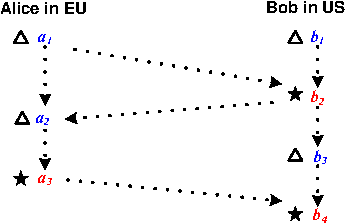
\includegraphics[width=0.9\columnwidth]{figures/redblue/redblueOrder/redblueGlobalOrder.pdf}
\label{fig:expositoryorder}
}
\end{minipage}
\par\bigskip
 \begin{minipage}[t]{0.5\columnwidth}
\centering
\subfloat[Causal serializations of $O$]{
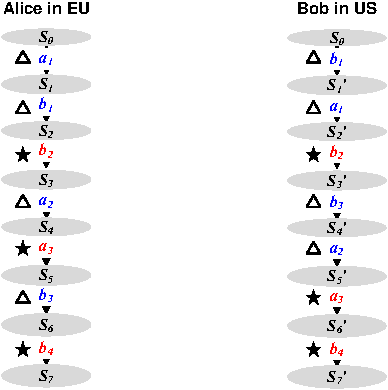
\includegraphics[width=1.0\columnwidth]{figures/redblue/redblueOrder/redblueOrderSerial.pdf}
\label{fig:expositoryexecutionorder}
}
\end{minipage}
\caption{\RBo\ and causal serializations for a system spanning two
  sites. \Operations\ marked with {\Large $\star$} are \red;
  \operations\ marked with $\bigtriangleup$ are \blue. Dotted arrows in \protect\subref{fig:expositoryorder} indicate
  dependencies between \operations. }
\label{fig:expositoryfigure}
\end{figure}

The definition of \RBc\ has two components:  
(1) A \RBo, which defines a (global) partial order of
\operations, and (2) a set of local causal
serializations, which define site-specific total orders
in which the \operations\ are locally applied.

\begin{mydef}[\RBo]
\label{def:rbo}
Given a set of \transactions\ $U=\R\cup \B$, where $\R\cap \B =
\emptyset$, a \emph{\RBo} is a partial order $O=(U,\prec)$ with the
restriction that $\forall u,v \in \R$ such that $u \neq v$, $u\prec v$
or $v\prec u$ (i.e., \red\ \operations\ are totally ordered).
\end{mydef}

Recall that each site is modeled as a deterministic state machine
capable of processing a totally ordered sequence of \operations. We
define which serializations are allowed for a given \RBo\ as follows:

\begin{mydef}[Legal serialization]
$O'=(U,<)$ is a {\em legal serialization} of \RBo\ $O=(U,\prec)$ if
\begin{itemize}
\item
$O'$ is a linear extension of $O$; i.e., $<$ is a total order
compatible with the partial order defined by $\prec$.
\end{itemize}
\label{def:legalserial}
\end{mydef}

This definition forces the serial order by which replicas execute
\operations\ to be compatible with the \RBo. However, it fails to
enforce causality, meaning that if an \operation\ $v$ sees the effects of \operation\ $u$ at its
primary site, then any \operation\ $w$ that sees the effects of $v$
must also see the effect of $u$ at all sites in the system.
In order to preserve causality, we extend the above
definition by saying that if \operation\ $v$ sees the effects of $u$
at its primary site, \site{v}, then  $u$ must be serialized before $v$ at all sites.

\begin{mydef}[Causal legal serialization]
  Given a site $i$, $O_i=(U,<)$ is an {\em $i$-causal legal serialization}
  (or short, a \emph{causal serialization}) of \RBo\ $O=(U,\prec)$ if
 \begin{itemize} 
  \item $O_i$ is a legal serialization of $O$, and 
  \item for any two \operations\ $u,v\in U$, if $\site{v}=i$ and $u<v$ in $O_i$, then
  $u\prec v$.
 \end{itemize}

\label{def:legalcausalserial}
\end{mydef}

A replicated system with
$k$ sites is then \RBct\ if every site applies a causal serialization
of the same global \RBo\ $O$.

\begin{mydef}[\RBc]
A replicated system is {\em $O$-\RBct} (or short, \RBct) if each site $i$ applies
operations according to an $i$-causal serialization of \RBo\ $O$.
\label{def:rbct}
\end{mydef}
%%%%%%%%% old version of the definition
\eat{
%\johannes{
\begin{mydef}[\RBc]
  A system is {\em $O$-\RBct} (or short, \RBct) if each site $i$ applies
operations according to an $i$-causal serialization of $O$.
%for all sites $i$, the state reached by site $i$ is the result of a
%site-$i$-causal serialization $O_i$ of the same \RBo\ $O$.
\label{def:rbct}
\end{mydef}
%}
}

Figure~\ref{fig:expositoryfigure} shows a \RBo\ and a pair of causal
serializations of that \RBo. In systems where every \operation\ is
labeled \red, \RBc\ is equivalent to
serializability~\cite{Bernstein1987CCR}; in systems where every
\operation\ is labeled \blue, \RBc\ allows the same set of behaviors as
causal consistency~\cite{Terry1995Managing,Lloyd2011Causal,
Mahajan2010Depot}. It is important to note that while \RBc\ constrains 
possible orderings of \operations\ at each site and thus the states the
system can reach, it does not ensure {\em a priori} that the system achieves 
all the end-to-end properties identified in Section~\ref{ch:redblue:sect:related}, 
namely, state convergence and invariant preservation, as discussed next.

\subsection{State convergence and a \RB\ bank}
\label{ch:redblue:sect:diverge}

In order to understand \RBc\ it is instructive to look at a concrete example. 
For this example, consider a simple bank with two users: Alice in the EU and Bob in the
US. Alice and Bob share a single bank account where they can deposit
or withdraw funds and where a local bank branch can accrue interest on
the account (pseudocode for the \operations\ can be found in
Figure~\ref{fig:bankPseudo}).  
Let the {\tt deposit} and {\tt accrueinterest} \operations\ be \blue.
Figure~\ref{fig:bankexample} shows a \RBo\ of deposits and interest
accruals made by Alice and Bob and two possible causal serializations applied at
both branches of the bank.

\begin{figure}[t]
\centering
\begin{minipage}{0.5\columnwidth}
%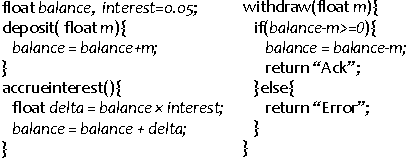
\includegraphics[width=1.0\columnwidth]{figures/redblueOrder/bankCode.pdf}
\pseudocodeinput[breaklines=true,mathescape=true]{pseudocode/redblue/basicexample.txt}
\end{minipage}
\caption{Pseudocode for the bank example.}
\label{fig:bankPseudo}
\end{figure}

\begin{figure}[t]
\centering
\begin{minipage}[t]{0.6\columnwidth}
\centering
\subfloat[\sf \RBo\ $O$ of \operations\ issued by Alice and Bob ]{
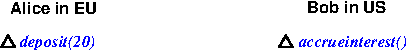
\includegraphics[width=0.9\columnwidth]{figures/redblue/redblueOrder/redblueOrderBank.pdf}
\label{fig:simplebankrbo}
}
\end{minipage}
\par\bigskip
\begin{minipage}[t]{0.6\columnwidth}
\centering
\subfloat[\sf Causal serializations of $O$ leading to diverged state]{
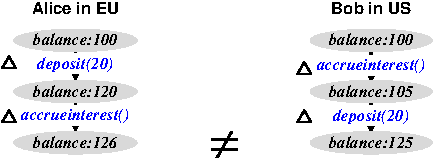
\includegraphics[width=1.0\columnwidth]{figures/redblue/redblueOrder/redblueOrderBankSerial.pdf}
\label{fig:divergestate}
}
\end{minipage}
\caption{A \RBct\ account with initial balance of \$100.}
% \changebars{and final diverged state}{}. \changebars{}{ (a) \RBo\ of
%  \operations\ issued by Alice and Bob. (b) Divergent causal serializations.}}
\label{fig:bankexample}
\end{figure}

State convergence is important for replicated systems. Intuitively a
pair of replicas is state convergent if, after processing the same
set of \operations, they are in the same state.  In the context of
\RBc\ we formalize state convergence as follows:

\begin{mydef}[State convergence]
A \RBct\ system is state convergent if all causal serializations of
the underlying \RBo\ $O$ reach the same state $S$ w.r.t any initial state $S_0$.
\end{mydef}

The bank example as described is not state convergent. The root cause is not surprising: \RBc\ allows
sites to execute \blue\ \operations\ in different orders but two
\blue\ \operations\ in the example correspond to non-commutative
operations---addition ({\tt dep\-osit}) and multiplication ({\tt accrueinterest}).
A sufficient condition to guarantee state convergence in a
\RBct\ system is that every \blue\ \operation\ is {\em globally commutative}, i.e., it commutes with all other
\operations, \blue\ or \red. We formally define this condition in the following
theorem.
%% \begin{theorem}
%%   For any \RBo\ $O=(U,\prec)$, if every 
%% %new
%% \changebars{\blue\ \operation\ is globally commutative, then $O$ is
%%   state convergent.}
%% %old
%% {pair of non-commutative \operations\ $u$ and $v$ are colored \red,
%%   then $O$ is state convergent.  }
%% %done
%% \footnote{All proofs will be found in a separated technical report,
%%   which is still under construction. \allen{This must be completed
%%     before we send the camera-ready.  EVen if it means simply
%%     uncommenting the text/proofs from the current TR forms}}
%% \label{them:commute}
%% \end{theorem}
%jg11: Suggest this new version of the theorem:

\begin{theorem}
Given a \RBo\ $O$, if all \blue\ \operations\ are globally commutative, then 
any $O$-\RBct\ system is state convergent.
\label{them:commute}
\end{theorem}

%%%%%new transition
In order to prove the above theorem, we introduce the following three lemmas along with 
their proofs.

The first lemma asserts that, given a legal serialization, swapping two
adjacent operations in the legal serialization that are not ordered by
the underlying \RBo\ results in another legal serialization.
\begin{lemma}\label{lem:canSwap}
Given a legal serialization $O_i=(U,<_i)$ of \RBo\ $O=(U,\prec)$
with \transactions\ $u,v\in U$ such that $u<_iv$ and $u \not\prec v$ and
there exists no $s$ such that $u<_{i}s<_{i}v$, and let $P=\{ p | p \in U \wedge p <_i u\}$
and $Q=\{q | q \in U \wedge v <_i q\}$. The serialization $O_k=(U,<_k)$ where
  \begin{itemize}
    \item $\forall p,q\in P \cup Q: p<_kq
      \Longleftrightarrow p<_iq$,
  \item $\forall p \in P: p <_k v$,
  \item $v<_k u$,
  \item $\forall q \in Q: u <_k q$
 \end{itemize}
 is a legal serialization.
 \end{lemma}

\noindent{\bf Proof:} It suffices to show that $\forall r,s \in U:$ $r<_k s$ is
   compatible with $\prec$. To do so, we consider the following six cases:

\begin{itemize}
\item {\bf Case 1:} $r,s\in P\cup Q$.  Since $O_i$ is a legal serialization,
each $r<_i s$ is compatible with $\prec$ by definition.  By
construction $\forall p,q\in P \cup Q:$ $r<_k s \Longleftrightarrow r<_i s$, so each $r<_k s$ is also compatible with $\prec$.

\item {\bf Case 2:} $r \in P$, $s = v$.  $r<_k s$ is compatible with $\prec$ by
similar logic as above.

\item {\bf Case 3:} $r = u$, $s \in Q$.  $r <_k s$ is compatible with $\prec$ by
 similar logic as above.

\item {\bf Case 4:} $v<_k u$.  Since $u\not\prec v$, $v<_k u$  is compatible with $\prec$. 

\item {\bf Case 5:} $r \in P$, $s = u$. Since $v <_{k} u \wedge \forall p \in P: p <_{k} v \implies p <_{k} u$. By the construction of $P$, $\forall p \in P: p <_{k} u \Longleftrightarrow p<_{i} u$. So each $r<_k s$ is also compatible with $\prec$.

\item {\bf Case 6:} $r = v$, $s \in Q$. Since $v <_{k} u \wedge \forall q \in Q: v <_{k} q \implies v <_{k} q$. $r <_k s$ is compatible with $\prec$ by
 similar logic as above.
\end{itemize}
As $U = P \cup Q \cup \{u,v\}$, by all above cases, $\forall r, s\in U:$ $r<_k s$ is compatible with $\prec$.\qed

%% Lemma 2: given a legal serialization and some pair of elements that
%% are unordered in the \rbo\, then there exists an adjacent pair of
%% elements that are not ordered.  (this ensures that the conditions for
%% lemma 1 are met)
The following lemma asserts that given a \RBo\ and its legal serialization, if there exists
a pair of elements that are not ordered by the \RBo, then there exists an adjacent
pair of elements between $u$ and $v$ in the legal serialization that are not ordered by the \RBo.

%The following lemma asserts that given two distinct legal
%serializations of the same \RBo, there exists an adjacent pair of
%operations in the first whose relative order in the second is
%reversed.

\begin{lemma}\label{lem:adjexists}
Given a legal serialization $O_i=(U,<_i)$ of \RBo\ $O=(U,\prec)$, if
$\exists u,v\in U$ such that $u<_i v$ and $u\not\prec v$,
let $U' = \{u,v\} \cup \{q|u<_i q\wedge q<_i v\}$, then $\exists r, s \in U'$ such that $r<_i s \wedge$ $r\not\prec s$ $\wedge \not\exists p \in U': r<_i p\wedge p <_i s$.
\end{lemma}
%% lemma 3: two legal serializations that differ in the order of one pair
%% of adjacent operations are convergent

\noindent{\bf Proof:}
We prove this by performing the following exhaustive analysis. The analysis
terminates when the required pair of elements is found.

Let's start with $u, v$. Consider $Q$ to be the sequence of elements strictly between $u$ and $v$, i.e.,
$Q=\{q\in U| u<_i q \wedge q <_i v\}$. There are two cases we have to analyze:
\begin{itemize}
\item {\bf Case 1:} $Q$ is empty. This implies that $u$ and $v$ are adjacent, so the analysis
terminates.

\item {\bf Case 2:} $Q$ is not empty. This implies that $u$ and $v$ are not adjacent.
Consider $p$ to be the first element in $U'$ according to $<_i$, i.e.,
$p\in U': \forall q\in U'\setminus\{p\}, p<_i q$. There are two cases to consider:
\begin{itemize}
\item {\bf Case 2a:} $u\not\prec p$. It follows that $p$ is the successor of $u$ in
$O_i$, then $u, p$ is the adjacent pair that are not ordered by $O$. The analysis
terminates.

\item {\bf Case 2b:} $u\prec p$. It follows from the assertion that $u\not\prec v$
and the transitivity of $\prec$ that $p\not\prec v$. Then we run
the analysis from the beginning with $p,v$. Since we are removing
the first element of the sequence $Q$, the analysis will either eventually
terminate with an empty sequence, or before that.
\end{itemize}
\end{itemize}
\qed


The third lemma asserts that two legal serializations that differ
in the order of exactly one pair of adjacent operations (one of which
is \blue) are state convergent, if all their \blue\ operations are globally
commutative.

\begin{lemma}\label{lem:adjacentconvergent}
Assume $O_i=(U,<_i)$ and $O_j=(U,<_j)$ are both legal
serializations of \RBo\ $O=(U,\prec)$ that are identical except for
two adjacent \transactions\ $u$ and $v$ such that $u<_iv$ and $v<_ju$ and that all
\blue\ operations $r\in U$ are globally commutative. Then
$S(O_i)=S(O_j)$.
\end{lemma}

\noindent{\bf Proof:} Let $P$ and $Q$ be the greatest common prefix and suffix
respectively of $O_i$ and $O_j$.  Further, let $S_P=S_0(P)$,
$S_{uv}=S_P+u+v$, and $S_{vu}=S_P+v+u$.

It follows from the definition of a \RBo\ (Definition~\ref{def:rbo}) and a legal serialization (Definition~\ref{def:legalserial})
that either $u\in B$ or $v\in B$.  Without loss of generality, assume
$u\in B$. By assumption $u$ commutes with all \transactions\ in $U$, therefore
$S_{uv}=S_{vu}$. It then follows the definition
of deterministic state machine that $S_{uv}(Q) = S_{vu}(Q)$. 
By the definition of legal serialization (Definition~\ref{def:legalserial}), 
the final state reached by sequentially executing operations in $O_{i}$ 
against $S$ according to $<$ is equal to the final state obtained by 
sequentially applying operations in $Q$ against $S_{uv}$ according to $<$, namely $S_0(O_i)=S_{uv}(Q)$. By
a similar argument, we know $S_0(O_j)=S_{vu}(Q)$. Finally, we have $S_0(O_i)=S_0(O_j)$.\qed


With the above lemmas, we could prove the state convergence theorem (Theorem~\ref{them:commute}) as follows:

\noindent{\bf Proof:} To prove a \RBct\ system is state convergent,
it is sufficient to show that for a \RBo\ $O$ of that system, any pair of its causal legal
serializations reaches the same final state w.r.t any initial state. To achieve
this, we take a slightly more conservative approach, which is to prove 
that any pair of legal serializations of their underlying \RBo\ $O$ is state convergent. 
Let $O_{i}$ and $O_{j}$ be two legal serializations of $O$. There are two cases to consider:

\begin{itemize}

\item {\bf Case 1:} $O_i = O_j$.  The underlying deterministic state
machine ensures that $S(O_i)=S(O_j)$.

\item {\bf Case 2:} $O_i \neq O_j$, in which case $\exists u,v\in U$
such that $u<_i v$ and $v<_j u$. Since both $O_i$ and $O_j$ are
legal serializations of $O$, it follows that $u\not\prec v$ and
$v\not\prec u$. It then follows Lemma~\ref{lem:adjexists} that we
can find an adjacent pair of operations $r, s$ such
that $r<_i s \wedge s<_j r \wedge r\not\prec s \wedge s\not\prec r$. We construct a new
serialization $O_{i+1}$ by first duplicating $O_i$ and then swapping the order of $r$ and $s$ in $O_{i+1}$, 
i.e., $r<_i s \wedge s<_{i+1} r$. By Lemma~\ref{lem:canSwap}, $O_{i+1}$ is 
also a legal serialization of $O$.

If $O_{i+1} \neq O_j$, we continue the construction by finding 
an adjacent pair of elements whose order is different in $O_{i+1}$, $O_j$. By swapping
the two operations, we obtain another legal serialization $O_{i+2}$. We can then continue to swap
all such adjacent pairs until the last constructed serialization
is equal to $O_j$. This is achievable since 
for any two legal serializations generated from two consecutive steps, $O'$ and $O''$,
the number of pairs in $O''$ whose orders
are different in $O_j$ becomes smaller than the number observed in $O'$.
At the end, the construction process results in a chain of legal
serializations where the first one is $O_i$ and the last is $O_j$, and any consecutive pair of legal serializations
is identical except for the order of an adjacent pair of elements. It then follows 
Lemma~\ref{lem:adjacentconvergent} and the assumption that
all \blue\ operations are globally commutative that every consecutive pair of
serializations in the chain is state convergent. Thus, $S_0(O_i)=S_0(O_j)$.\qed
\end{itemize}

Theorem~\ref{them:commute} highlights an important tension inherent to \RBc. On the one hand,
low latency requires an abundance of \blue\ \operations\ that can be
locally executed and lazily replicated. On the other hand, state
convergence requires that \blue\ \operations\ commute with all other
\operations, \blue\ or \red. In order to make the banking
example shown in Figure~\ref{fig:bankPseudo} and~\ref{fig:bankexample} converge, one has to label all three
operations \red, namely {\tt deposit}, {\tt withdraw} and {\tt accrueinterest}.
Obviously, this labeling will lead to a significant performance penalty, due
all operations must be serialized w.r.t each other. The poor result
implies that there exists an obstacle to making systems fast under \RBCN, which
is that the number of commuting operations in the real world is quite limited. 
As a result, in the following section
we introduce a method for addressing this tension by significantly
increasing the amount of commutativity in application \operations.

\section{Replicating side effects}
\label{ch:redblue:sect:shadowops}

In this section, we observe that while \operations\ themselves
may not be commutative, \emph{we can often make the chan\-ges they
  induce on the system state commute.}  Let us illustrate this issue
within the context of the \RedBlue\ bank from Section~\ref{ch:redblue:sect:diverge}.
We can make the {\tt deposit} and {\tt accrueinterest}
\operations\ commute by first computing the amount of interested accrued
and then treating that value as a deposit.

\subsection{Defining \shadow\ \operations}
\label{sect:defineshadow}

The key idea is to split each original application \operation\ $u$
into two components: a {\em \initial\ \operation} $g_u$ with no
side-effects, which is executed only at the primary site against some
system state $S$ and produces a {\em \shadow\ \operation} $h_u(S)$,
which is executed at every site (including the primary site). The
\initial\ \operation\ decides which state transitions should be made
while the \shadow\ \operation\ applies the transitions in a
state-indep\-endent manner.

The simplest way of making such a decomposition is generating
a no-op shadow operation for every original operation. Although this strategy makes every
shadow operation globally commutative and potentially \blue,
it delivers a completely unmeaningful service. In order to follow the 
intended application semantics, one cannot
split original operations in an arbitrary manner: 
the implementation of \initial\ and \shadow\ \operations\ must obey some basic
correctness requirements. First, \initial\ \operations, as mentioned, must
not have any side effects. Furthermore, \shadow\ \operations\ must produce
the same effects as the corresponding original \operation\ when
executed against the original state $S$  used as an argument
in the creation of the \shadow\ \operation. More formally:

\begin{mydef}[Correct \initial\ / \shadow\ \operations]
The decomposition of \operation\ $u$ into \initial\ and sh\-adow
\operations\ is correct if for all states $S$, the
\initial\ \operation\ $g_u$ has no effect and the generated
\shadow\ \operation\ $h_u(S)$ has the same effect as $u$ w.r.t $S$, i.e., for
any state $S$: $S+g_u = S$ and $S+h_u(S) = S+u$.
\label{def:correctshadow}
\end{mydef}

Note that a trivial decomposition of an original \operation\ $u$ 
into \initial\ and \shadow\ \operations\ is to let $g_u$ be a no-op and let $h_u(S) = u$
for all $S$. This is correct but it does not increase the space
of commutativity. Later in this chapter, we will present a few
examples, in which we made an effort to produce commutative shadow operations.

In practice, as exemplified in Section~\ref{ch:redblue:sect:casestudies}, separating
the decision of which transition to make from the act of applying the
transition allows many objects and their associated usage in
\shadow\ \operations\ to form an abelian group and thus dramatically
increase the number of commutative (i.e., \blue) \operations\ in the
system. Furthermore, unlike previous approaches
\cite{Gray1996Dangers,Shapiro2011Conflict}, for a given
  original operation, our solution allows its \initial\ operation
to generate state-specific \shadow\ operations with different
properties, which can then be assigned different colors in the
\RBc\ model.

\subsection{Revisiting \RBc}
\label{sect:rbcimplications}
The key insight that underlies \shadow\ \operations\ is breaking
  the execution of an \operation\ down into the decide (\initial) and
  apply (\shadow) phases.  This decomposition, however, requires us to revisit the
  foundations of \RBc. In particular, only \shadow\ \operations\ are included in a
  \RBo\ while the causal serialization for site $i$ additionally includes the \initial\ \operations\ initially
  executed at site $i$. The causal serialization must ensure that
  \initial\ \operations\ see the same state that is associated with
  the generated \shadow\ \operation\ and that
  \shadow\ \operations\ appropriately inherit all dependencies from
  their \initial\ \operation.

\if 0
%new
\changebars{Decomposing \operations\ into \initial\ and
  \shadow\ components requires us to revisit the foundations of
  \RBc. In particular, only \shadow\ \operations\ are included in a
  \RBo\ while the causal serialization for site $i$ additionally includes the \initial\ \operations\ initially
  executed at site $i$.  The causal serialization must ensure that
  \initial\ \operations\ see the same state that is associated with
  the generated \shadow\ \operation\ and that
  \shadow\ \operations\ appropriately inherit all dependencies from
  \changebars{their}{the associated} \initial\ \operation.}
%old
{ The key insight that underlies \shadow\ \operations\ is breaking
  execution of an \operation\ down into the decide (\initial) and
  apply (\shadow) phases.  This, however, causes us to revisit the
  definitions behind \RBc. In particular, the notion of causal legal
  serialization, which is at the core of the definition of \RBc, now
  needs to take into account not only the admissible serializations
  under which \shadow\ \operations\ can be executed, but also the
  points in the serialization where \initial\ \operations\ can be
  interleaved, and consequently the state $S$ that they observe and
  that becomes associated with the corresponding \shadow\ \operation.
  In the new definition, \shadow\ \operations\ need to obey the
  restrictions of causal legal serializations.  Furthermore, we must
  restrict the state seen associated with \shadow\ \operations\ to
  match the state seen be the corresponding \initial\ \operation.
  Finally, \initial\ executions must be compatible with the \RBo\ and
  also preserve causality, similarly to the previous notion of causal
  legal serialization. In particular, the operations that precede a
  \initial\ \operation\ must be the same that precede the
  corresponding \shadow\ operation in the \RBo. This ensures that the
  operations that see this \shadow\ \operation\ also see the
  \operations\ that the corresponding \initial\ \operation\ saw.  }
\fi
%% \rodrigo{Previous lead paragraph:

%% The key insight that underlies \shadow\ \operations\ is breaking
%% execution of an \operation\ down into the decide (\initial) and apply
%% (\shadow) phases. This decomposition 
%% requires us to revisit the foundations of \RBc.  When employing
%% \initial\ and \shadow\ \operations, only \shadow\ \operations\ are
%% labeled and included in the global \RBo\ and legal serializations
%% describing the states that each site may reach.  The causal legal
%% serialization, however, explicitly incorporates both \shadow\ and
%% \initial\ \operations.  A causal  serialization for site $i$
%% identifies the total order in which \shadow\ \operations\ are applied
%% at the site as well as the states against which locally executed
%% \initial\ \operations\ are executed to produce \shadow\ \operations.
%% We note that while \initial\ \operations\ produce
%% \shadow\ \operations, they do not change the system state.
%% }


We capture these subtleties in the following revised
  definition of causal serializations.  Let $U$ be the set of
\shadow\ \operations\ executed by the system and $V_i$ be the
\initial\ \operations\ executed at site $i$.
Note that the definitions of legal serialization and
  \RBo\ remain fundamentally unchanged, once ``\operation'' is
  replaced with ``\shadow\ \operation.''
\begin{mydef}[Causal serialization--revised]
Given a site $i$, $O_i=(U\cup V_i, <)$ is an $i$-causal serialization
of \RBo\ $O=(U,\prec)$ if
\begin{itemize}
%\setlength{\itemindent}{\itemindentsize}
%\setlength{\leftmargin}{0.25in}
\item $O_i$ is a total order;
\item $(U,<)$ is a linear extension of $O$;
\item For any $h_v(S)\in U$ generated by $g_v\in V_i$, $S$ is the
  state obtained after applying the sequence of
  \shadow\ \operations\ preceding $g_v$ in $O_i$;
\item For any $g_v\in V_i$ and $h_u(S), h_v(S') \in U$, $h_u(S)<g_v$ in $O_i$
  iff $h_u(S) \prec h_v(S')$ in $O$.
\end{itemize}
\label{def:shadowcausal}
\end{mydef}

%% \begin{definition}[Causal \changebars{}{legal} serialization (revised)]
%% The total order $O^*_i=(U\cup V_i,<)$ is a causal \changebars{}{legal}
%% serialization at site $i$ of \RBo\ $ O = (U,\prec)$ if
%% \begin{itemize}[leftmargin=0cm,itemindent=.5cm,labelwidth=\itemindent,labelsep=0cm,align=left]
%%   \setlength{\itemsep}{1pt}
%%   %\setlength{\parskip}{0pt}
%%   \setlength{\parsep}{0pt}
%% \item The restriction of $<$ on the set $U$ is a linear extension of
%%   $\prec$.
%% \item For any \shadow\ \operation\ $h_v(S)\in U$ generated by
%%    \initial\ \operation\ $g_v\in V_i$, $S$ is the state obtained after
%%   applying the sequence of \shadow\ \operations\ preceding $g_v$ in
%%   $O_i$.
%% \item For any \initial\ \operation\  $g_v\in V_i$ and
%%    \shadow\ \operation\ $h_u(S) \in U$, $h_u(S)<g_v$ in
%%   $O_i$ iff $h_u(S) \prec h_v(S')$ in $O$.
%% \end{itemize}
%% \end{definition}

Note that \shadow\ \operations\ appear in every
  causal serialization, while \initial\ \operations\ appear only in
  the causal serialization of the initially executing site.
  
 \begin{figure}[!t]
\centering
\begin{minipage}{0.5\columnwidth}
\pseudocodeinput[breaklines=true,mathescape=true]{pseudocode/redblue/advancedexample.txt}
\end{minipage}
\caption{Pseudocode for \shadow\ bank \operations.}
\label{fig:bankshadowcode}
\end{figure}

\begin{figure}[t]
\centering
\begin{minipage}[t]{0.6\columnwidth}
\centering
\subfloat[\textsf{\RBo\ $O$ of banking \shadow\ \operations}]{
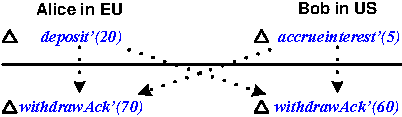
\includegraphics[width=1.0\columnwidth]{figures/redblue/redblueOrder/redblueOrderBankAllBlue.pdf}
\label{fig:shadowopRBO}
}
\end{minipage}
\par\bigskip
\begin{minipage}[t]{0.75\columnwidth}
\centering
\subfloat[\textsf{Invalid but convergent causal serializations of $O$}]{
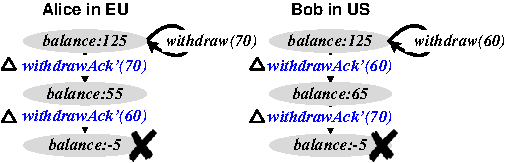
\includegraphics[width=1.0\columnwidth]{figures/redblue/redblueOrder/redblueOrderBankShadowSerialInv.pdf}
\label{fig:shadowopLegal}
}
\end{minipage}
\caption{ A \RBct\ bank with only \blue\ \operations.
%%\changebars{A \RBct\ bank with all \red\ \shadow\ \operations\ and reaches an invalid state}{ (a) \RBo\ of banking \shadow\ \operations.  (b) Convergent
 % causal serializations that result in an invalid state}; The
  The starting balance of \$125 is the result of applying
  \shadow\ \operations\ above the solid line to an initial balance of
  \$100.  Loops indicate \initial\ \operations.}
\label{fig:shadowopfigure}
\end{figure}

\subsection{\Shadow\ banking and invariants}
\label{sect:shadowbank}



Figure~\ref{fig:bankshadowcode} shows the \shadow\ \operations\ for
the banking example. Note that the {\tt with\-draw} \operation\ maps
to two distinct \shadow\ \operations\ that may be labeled as \blue\ or \red\ indep\-endently---{\tt with\-drawAck'} and
{\tt with\-drawFail'}. {\tt withdrawAck'} refers to successful withdrawal,
while {\tt withdrawFail'} corresponds to failure due the balance value is not enough.

Figure~\ref{fig:shadowopfigure}
illustrates that \shadow\ \operations\ make it possible
for all \operations\ to commute, provided that we can identify the
underlying abelian group. This does not mean, however,
  that it is safe to label all \operations\ \blue.
%new
%\changebars{Figure~\ref{fig:shadowopfigure} shows the impact of
%  labeling all four \shadow\ \operations\ in the bank example \blue,
%  including {\tt withdrawAck'}. Starting with an initial balance of
%  \$125 (based on the example from Figure~\ref{fig:bankexample}),
%  Alice and Bob successfully, and independently, withdraw \$70 and
%  \$60 respectively from their local branches.  When the
%  \shadow\ \operations\ are exchanged, both branches will show a
In this example (Figure~\ref{fig:shadowopfigure}\subref{fig:shadowopLegal}), such a labeling would allow Alice and Bob to successfully
  withdraw \$70 and \$60 at their local branches, thus ending up with
a final balance of \$-5. This violates the
  fundamental invariant that a bank balance should never be negative.

To determine which operations can be safely labeled
\blue, we begin by defining that a \shadow\ \operation\ is invariant safe if,
  when applied to a valid state, it always transitions the system into
  another valid state.

\begin{mydef}[Invariant safe] \Shadow\ \operation\ $h_u(S)$ is invariant
  safe if for all valid states $S$ and $ S'$, the state $S'+h_u(S)$ is
  also valid.
\label{def:isafeop}
\end{mydef}
%new

We also assume that the original applications without being \RBct\ replicated
are correct, i.e., all their original operations always transition
from a valid system state to another valid state. This is captured by the following
trivial definition:

%\newchange{Before adapting a system to be \RBct, we have to 
%assert all its original operations are correct.}

\begin{mydef}[Correct original operation]
Original operation $t$ is correct if for
all valid states $S$, $S + t$ is also valid.
\label{def:correctoriginal}
\end{mydef}

The following theorem states that in a \RBct\ system with
  appropriate labeling, each replica transitions only through valid
  states. 

%\newchange{Cheng: modified the original theorem by adding two things
%a) we assert all its original operations are correct; and
%b) any execution of the system starts from a valid state.}

\begin{theorem}
Given a \RBct\ system,
  if every original operation and any pair of \initial\ and \shadow\ \operations\ is correct 
and all its \blue\ \shadow\ \operations\ are invariant safe and globally
  commutative, then for any execution of that system that starts
from a valid state, no
  site is ever in an invalid state.
\label{them:safe}
\end{theorem}

It is worth noting that this theorem highlights a non-obvious
result: even \red\ \shadow\ \operations\ that may break invariants are allowed
to be applied against completely different state, provided that those \operations\ are
serialized w.r.t each other in the same order at all sites (but not w.r.t
the remaining ones).

\if 0
\techReportOnly{\noindent{\bf Proof.} Let $O=(U,\prec)$ be a \RBo\ and $U=B
  \cup R$ such that $\forall u \in U$ is correct and $\forall v \in B$
  is invariant safe and globally commutative. Let $L$ be a legal
  serialization of $O$.  We proceed by induction on the number of
  \shadow\ \operations\ in $U$.

{\bf Base case:} There is no non-empty prefix $P$ of $L$ such that the
state reached by $P$ is not valid; included in this condition is
$|U|=0$.  The theorem is proved.

{\bf Inductive step (by Contradiction):} There exists a non-empty prefix $P$ of $L$ such
that the state reached by $P$ is not valid.  Further, let $P$ be the
shortest such prefix.  Let $u$ be the last operation in $P$ such that
$P=P'+u$.  We know by assumption that $P$ is the shortest prefix of
$L$ such that the state reached by $P$ is not valid, so the state
reached by $P'$ must be valid.  Further, $P$ is a legal serialization
of $O'=(U',\prec)$ where $O'$ is a prefix of $O$.

{\bf Case 1:} Let $u$ be \blue.  By assertion, $u$ is invariant safe.
It thus follows from the observation that the state reached by $P'$ is
valid that the state reached by $P$ is also valid, violating the
assumption that the state reached by $P$ is not valid.  Therefore $u$
must be \red.

{\bf Case 2:} Let $u=h_t(S^*)$ be \red\ and $S^*$ be the state
reached by $P'$. It follows from the definition of a correct
\shadow\ operation that $S^*+u=$ is the state reached by $P$ and is a valid state, violating the
assertion that the state reached by $P$ is not valid.  Therefore $u$ must be \red\ and the state reached by $P$ is not $S^*$.

{\bf Case 3:} Let $u=h_t(S^*)$ be \red\ and the state reached by $P$
be $S'\neq S^*$.  It follows from the definitions of a \RBo\ and a
legal serialization that there exists a
\blue\ \shadow\ \transaction\ $v$ such that $u<_U v$ and $u\not\prec_O
v\wedge v\not\prec_O u$.  It then follows from
Lemmas~\ref{lem:canSwap} and~\ref{lem:adjexists} that we can
construct a legal serialization $T$ of $O$ where the last two elements
of $T$, in order, are $u$ and $v$.  It follows from
Theorem~\ref{them:commute} that $T$ and $P$ are state convergent.  Let
$T=T'+v$.  Since $v$ is an invariant safe
\blue\ \shadow\ \operation\ and the state reached by $T$ is not state,
it follows that the state reached by $T'$ is also not valid. We
proceed by induction on $O''=(U','\prec)$ where $U''=U'\setminus\{v\}$ and $|U''|<|U|$.\qed}

\fi


\begin{figure}[!t]
\centering
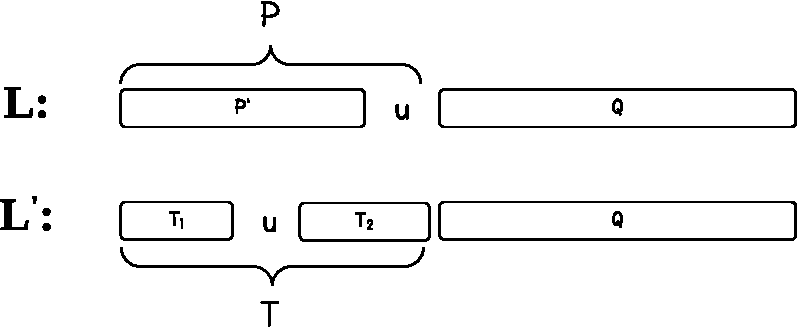
\includegraphics[width=0.76\columnwidth]{figures/redblue/legal_serial_order_construction.pdf}
\caption{Two legal serializations $L$ and $L'$. $L'$ is constructed by
swapping every shadow operation $v$ in $P'$ and $u$ if $u$ and $v$ are not partially ordered.}
\label{fig:invpreserve_example}
\end{figure}

%%%%new proof starts
%\newchange{Cheng: the proof is new.}

\noindent {\bf Proof by contradiction.} Let $O=(U,\prec)$ be a \RBo\ and $U=B
  \cup R$, where $B$ and $R$ denotes the \blue\ or \red\ shadow operation set, 
respectively. For every shadow operation $u$ in $U$, $u$'s original operation is correct
and the corresponding decomposition is correct. 
Every \blue\ shadow operation $v$, i.e., $v \in B$,
  is invariant safe and globally commutative. The initial state $S_0$ is valid. 	

Let $L$ be a causal serialization of $O$, which is shown in 
Figure~\ref{fig:invpreserve_example}. Assume that $L$ is in an invalid state.
We prove this theorem by performing the following exhaustive analysis
and showing the contradictions found. 

Analysis: Let $P(U_P, <_P)$ be the shortest prefix of $L$ that produces 
an invalid state. If $P$ is empty, 
then $S_0(P) = S_0$, and $L$ is in a valid state.
This violates the assumption that $L$ is in an invalid state. The theorem is proved.

If $P$ is non-empty, then consider $u$ to be the last shadow operation in $P$ such that
$P=P'+u$, where $P'$ is a prefix of $P$. Let $t$ be the original operation of $u$. By the definition of 
shadow operation, we know $u=h_t(S')$, where $S'$ is the state in which $u$ was
generated. There are two cases we need to consider:
\begin{itemize}
\item {\bf Case 1:} $u$ is \blue. As every \blue\ shadow operation is invariant safe, 
the state reached before applying $u$, $S_0(P')$, must be invalid. This contradicts
the assumption that $P$ is the shortest prefix that introduces an invalid state. The theorem
is proved.

\item {\bf Case 2:} $u$ is \red. $S'$ has two possible values.
\begin{itemize}
\item {\bf Case 2a:} $S' = S_0(P')$, i.e., the state that $u$ was applied against
is the same as the state that $u$ was created from. It follows from
the correct generator/shadow operation definition (Definition~\ref{def:correctshadow})
that $S' + u = S' + t$ and $S' + t$ is invalid. 
It then follows the correct original operation definition (Definition~\ref{def:correctoriginal})
 that $S'$ must be invalid as well. By the same
logic in Case 1, we found a shorter prefix $P'$ other than $P$ that
produces an invalid state. By contradiction, the theorem is proved.

\item {\bf Case 2b:} $S' \neq S_0(P')$. It follows the definition of \RBo\ (Definition~\ref{def:rbo}) and
causal serialization (Definition~\ref{def:shadowcausal}) that there exists some \blue\ \shadow\ \transactions\ $v$
that precede $u$ in $L$ but are not partially ordered with $u$ in $O$, 
i.e., $v<_Lu$ and $u\not\prec_{O} v\wedge v\not\prec_{O} u$. It then follows 
Lemmas~\ref{lem:canSwap} and~\ref{lem:adjexists} that we can
construct a new causal serialization $L'$ of $O$ by duplicating $L$ and
swapping the order between $u$ and every $v$ in $L'$, so that $u$ is bubbled up
over every such $v$. The result is shown in Figure~\ref{fig:invpreserve_example}.
The only difference between $L$ and $L'$ is as follows:
$\forall i \in U_{p}: i<_L u \wedge i\not\prec_{O} u \implies u<_{L'} i$. 
$T_1$ represents a sequence of shadow operations that precede $u$
in $O$, while $T_2$ represents a sequence of \blue\ shadow operations
that are not partially ordered with $u$.
By the state convergence theorem (Theorem~\ref{them:commute}) and the assumption that
every \blue\ shadow operation is globally commutative, so the prefix $T$ and $P$ must be state convergent, 
i.e., $S_0(P) = S_0(T)$. As $S_0(P)$ is invalid, $S_0(T)$ is also invalid. 

By the deterministic state machine model, we know
$S_0(T) = S_0(T_1) + u + T_2$, where as shown in Figure~\ref{fig:invpreserve_example}
$T_1$ and $T_2$ are the aforementioned prefix and suffix of $T$, respectively. As all \blue\
shadow operations are invariant safe, $S_0(T_1) + u$ must be invalid.
By the causal serialization definition (Definition~\ref{def:shadowcausal})
and the construction of $L'$, the state $S_0(T_1)$ is the state 
in which $u$ was generated. It then follows the correct generator/shadow operation
definition (Definition~\ref{def:correctshadow}) that $S_0(T_1) + u = S_0(T_1) + t$. It then follows
from the correct original operation definition (Definition~\ref{def:correctoriginal}) that $S_0(T_1)$ must be invalid as well. 
We proceed by starting again the analysis using as the input a new causal serialization
of $O$ and a new shortest prefix that produces an invalid state, i.e., $P=T_1 \wedge L = L'$.
This analysis is guaranteed to terminate since the size of $P$ at every subsequent analysis step
decreases.
\end{itemize}
\end{itemize}
\qed
%%%%%new proof ends

\begin{figure}[t!]
\centering
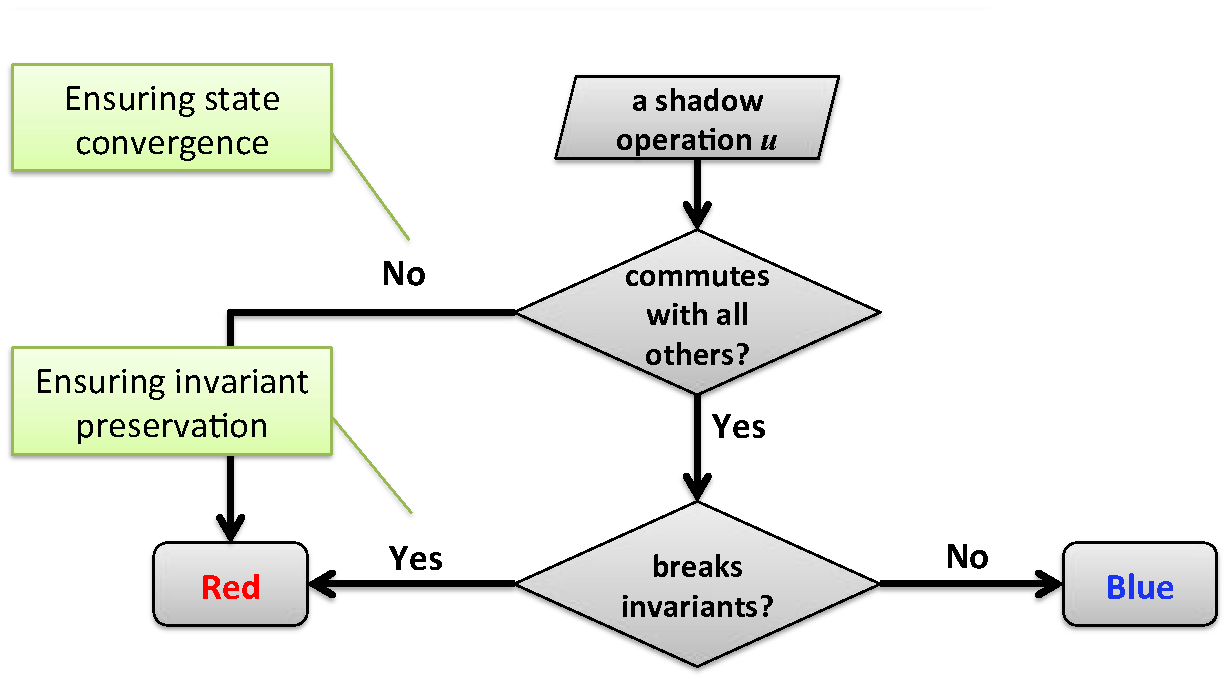
\includegraphics[width=0.86\columnwidth]{figures/redblue/principle_diagram.pdf}
\caption{Labeling methodology diagram.}
\label{fig:redbluelabeling}
\end{figure}


\subsection{What can be \blue?  What must be \red?}  
\label{ch:redblue:sect:labelmethod}
As illustrated by Theorem~\ref{them:commute},
the sufficient condition of ensuring the state convergence property is
that a shadow operation must be labeled as \red\ if it is not
globally commutative. The second theorem (Theorem~\ref{them:safe}) states
that invariants are maintained if all non-invariant safe shadow
operations are serialized. In summary, the combination of these two theorems
leads to the following procedure (shown in Figure~\ref{fig:redbluelabeling}) for deciding which \shadow\ \operations\ can be
\blue\ or must be \red\ if a \RBct\ system is to provide both
state convergence and invariant preservation:
\begin{enumerate}%[leftmargin=0cm,itemindent=.5cm,labelwidth=\itemindent,labelsep=0cm,align=left]
\item For any pair of non-commutative \shadow\ \transactions\ $u$ and $v$, label both $u$ and $v$ \red.
\item For any \shadow\ \transaction\ $u$ that may result in an invariant being
  violated, label $u$ \red.
\item Label all non-\red\ \shadow\ \transactions\ \blue.
\end{enumerate}

\begin{figure}[t!]
\centering 
\begin{minipage}[t]{0.56\columnwidth}
\centering
\subfloat[\sf \RBo\ $O$ of banking \shadow\ \operations]{
  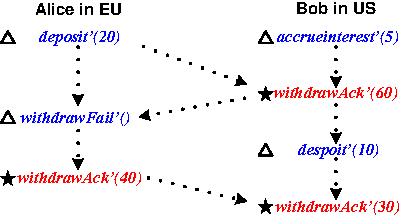
\includegraphics[width=1.0\columnwidth]{figures/redblue/redblueOrder/redblueOrderBankFinal.pdf}
\label{fig:shadowopRBO}
}
\end{minipage}
\par\bigskip
\begin{minipage}[t]{0.76\columnwidth}
\centering
\subfloat[\sf Convergent and invariant preserving causal serializations of $O$ ]{
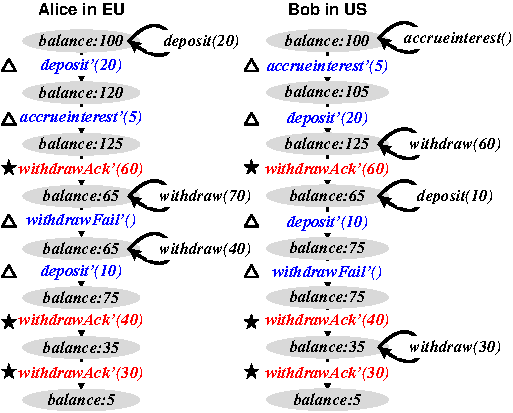
\includegraphics[width=1.0\columnwidth]{figures/redblue/redblueOrder/redblueOrderBankShadowSerialFinal.pdf}
\label{fig:shadowopLegal}
}
\end{minipage}
\caption{A \RBct\ bank with correctly labeled \shadow\ \operations\
  and initial balance of \$100.}
\label{fig:shadowopfinalfigure}
\end{figure}

Applying this decision process to the bank example leads to a 
labeling where {\tt withdrawAck'} is \red\ and the remaining
\shadow\ \operations\ are \blue. The only restriction we placed
is to make any pair of successful withdraw shadow operations
 be partially ordered, i.e., one must see
the effect introduced by another. Figure~\ref{fig:shadowopfinalfigure}
shows a \RBo\ with appropriately labeled \shadow\ \transactions\ and
causal serializations for the two sites that converge
to the same valid final state. In this example, the first {\tt withdraw} operation
issued by Alice in the EU site cannot proceed even provided that her local balance is enough
to complete this withdrawal. Instead, the execution must wait until the changes carried by the
\shadow\ \operation\ {\tt withdrawAck'(60)} from US have been made visible at the EU replica.
Upon this, the \initial\ of Alice's {\tt withdraw(70)} reads
the current balance value and produces a failure withdrawal (\blue). In the end,
the balance value remains non-negative.

\subsection{Discussion}
\label{sect:discussshadow}

\Shadow\ \operations\ and \RBCN\ introduce some surprising anomalies to a user
experience. Notably, while the effect of every user action is applied
at every site, the final system state is not guaranteed to match the
state resulting from a serial ordering of the original \operations.
The important thing to keep in mind is that the decisions made always
make sense in the context of the {\em local} view of the system: when
Alice accrues interest in the EU, the amount of interest accrued is
based on the balance that Alice observes at that moment.  If Bob
concurrently makes a deposit in the US and subsequently observes that
interest has been accrued, the amount of interest {\em will not} match
the amount that Bob would accrue based on the balance as he currently
observes it.

As such, \shadow\ \operations\ always provide for a coherent sequence of state
transitions that reflects the effects demanded by user activity; while
this sequence of state transitions is coherent (and convergent), the
state transitions are chosen based on the locally observable state
when/wh\-ere the user activity initiated and not the system state when
they are applied.

%\rodrigo{The next paragraph is a bit redundant with the first one.
%Given space constrains I suggest removing it and incorporating any
%missing points in the first paragraph.}

%While \RBc\ provides serializability in the context of \shadow
%\operations, it does not provide the same guarantees or intuitive
%understanding when considering the corresponding native \operations.
%What \RBc\ does provide is a causally consistent sequence of {\em
%  decisions} on which state transition to make and a sequentially
%consistent sequence of {\em applications} of the selected state
%transitions.  This can lead to situations where a user would
%reasonably expect a different outcome when executing a native
%\operation\ at a remote site.  




%% \allen{At this point (possibly in the RBC section instead?) we need a
%%   discussion of what RBC means to a user?  At least one reviewer was
%%   confused by the implications of causality and confusion over ``does
%%   this interest calculation make sense?  Would that discussion be
%%   appropriate here, with the below points on labeling moving into the
%%   beginning of case studies?  This discussion should also explicitly
%%   note that all \red\ is sequential consistency.}





\section{\gemini\ design \& implementation}
\label{ch:redblue:sect:gemini}

In this section we describe the design and implementation of
  \gemini, a prototype architecture that enables applications to run
  under \RBc.

\subsection{Design rationale}
As we saw in Section~\ref{ch:redblue:sect:casestudies},
some original operations may produce either \blue\ or \red\ \shadow\ \operations\
depending on the current system state and the user input they are observing. 
A nav{\" i}e solution would be to coordinate all generator operations that may produce
a \red\ shadow. This solution imposes more restrictions than
what \RBCN\ exactly needs, i.e., all relevant \shadow\ \operations\ even including
those blue ones would be serialized w.r.t each other. As a result, it
offsets the goal of \RBCN\ of only paying a performance penalty when strong consistency
is needed. To avoid this, we instead optimistically run 
the \initial\ \operation\ at its primary site in the first place,
and then speculatively generate a tentative shadow operation based on the local state and user input.
If the corresponding \shadow\ \operation\ is \blue, then a reply will be produced locally without
contacting remote replicas; Otherwise, replicas have to speak to
each other for establishing a total order among all \red\ shadow operations that are received,
and making sure that this \shadow\ \operation\ is generated
from a state reflecting all side effects introduced by all its preceding shadow operations. Therefore,
a \red\ tentative \shadow\ \operation\ might rollback, when the local state
is different from the global state due to conflicts, and we need to restart
the process of generating another shadow operation.

\begin{figure}[t!]
  \centering
    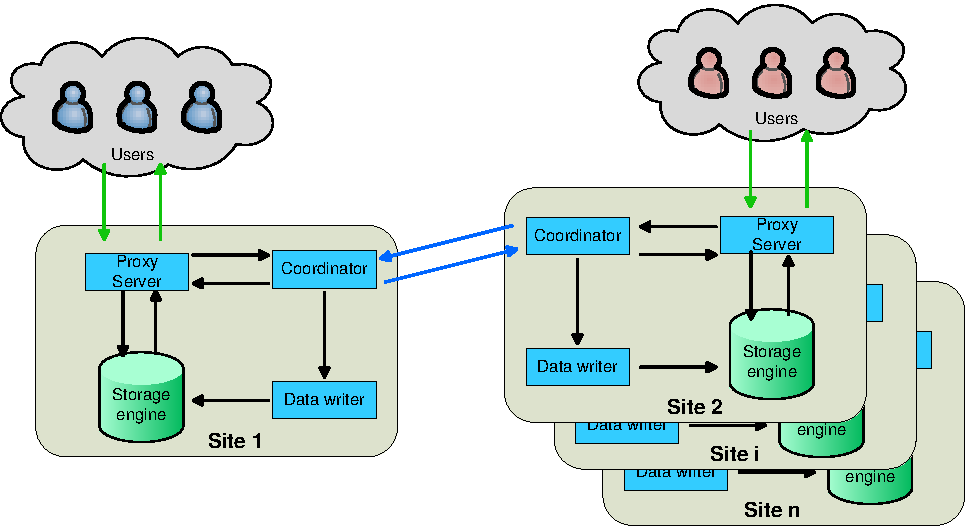
\includegraphics[width=0.95\columnwidth]{figures/redblue/GeminiArchi.pdf}
  \caption{Gemini system architecture. Blue arrows represent communication between sites,
black arrows indicate communication between system components within a site, and green
arrows correspond to communication between users and the replicated service.}
 \label{fig:geminiMultiDC}
\end{figure}

In addition, there are two requirements of executing generator operations: 1) they should
not interfere with other concurrent \transactions; and 2) there is no
need for them to make their identified side effects persistent. 
Given these observations, using a lock-based
concurrency control solution would be very conservative, since
granting locks to an \transaction\ may prevent other \transactions\ from making progress.
In summary, we resort to a form of optimistic concurrency control
(OCC)~\cite{Bernstein1987CCR} in \gemini, as we describe next. 
It is worth mentioning that the \gemini\ OCC slightly
deviates from the traditional textbook algorithm, since
our algorithm recognizes the fact that concurrent
\blue\ \shadow\ \operations\ are never conflicting with
all other \shadow\ \operations.

\if 0
In addition, under the \RBc\ model, \blue\ \transactions\ can never
conflict since they are assumed to concurrent red \transactions\ are
never conflicting with each other since they commute. In addition,
\initial\ \transactions\ should not interfere with other concurrent
\transactions.  Given these observations, using a lock-based
concurrency control solution would be very conservative, since
granting locks to a \transaction\ prevents other \transactions\ from
processing. As a result, we resort to optimistic concurrency control
(OCC)~\cite{Bernstein1987CCR} in \gemini, as we describe next.

\changebars{}
{
%\paragraph
{Extending commutativity}
% Identifying invariants requires us to analyze applications' sourcecode. The focus of this process is to check two essential parts of sourcecode normally used to express application invariants: \emph{if} statements embraced by synchronized primitives, and restrictions defined over data schemas (e.g., AUTOINCREMENT, UNIQUE attributes in MySQL). By doing so, we quickly identified two common invariants: a) id assigned must be unique; and b) the value of some state should not be negative.
We also observed that some \transactions\ were not immediately commutative due to implementation issues rather than to intrinsic non-commu-tativity issues.
One example is the implementation of uni-que identifiers---in the base centralized application we have used, unique identifiers are assigned using a monotonic counter stored in the database.
%When using this approach in our system, if the identifier is generated in the initial \transaction, concurrent initial \transactions\ running in %different sites could generate the same identifier. If the identifier is generated in the \shadow\ \transaction, \shadow\ \transactions would have %to execute in the same order in all replicas - i.e., they should be labeled blue.
We addressed this issue by associating each unique identifier with a site-specific prefix so that it is globally unique.
A second example is the case where commutativity is impeded by non-determinism in the operations executed in a transaction. This negative %impact can be easily solved by solving the non-determinism in the initial transaction and encoding the expected result into \shadow\ \operation.
impact can be easily solved by encoding the results produced by these operations into the corresponding \shadow\ \operations.
}
\fi

%As shown in Figure~\ref{fig:geminiMultiDC}, a single-site
%\nuno{************* new try starts here *************************************************************}

\subsection{System overview}
We implemented the \gemini\ storage system to provide \RBc. As shown in Figure~\ref{fig:geminiMultiDC}, each \gemini\ site consists of four components:
a storage engine, a proxy server, a concurrency coordinator, and a
 data writer. A multi-site deployment is constructed by replicating
 the single data center components across multiple sites.

The basic flow of user requests through the system is straightforward.
A user issues requests to a {\em proxy server} located at the closest
site. The proxy server processes a request by executing the \initial\ \operation\ of an
appropriate application transaction, which is implemented as a single
\gemini\ original \operation, comprising multiple data accesses; individual
data accesses within a \initial\ \operation\ execute in a temporary
private scratchpad, providing a virtual private copy of
  the service state. The original data lies in a {\em storage engine}, which provides a standard
storage interface. In our implementation, the storage
  engine is a relational database, and scratchpad operations are
  executed against a set of non-shared in-memory tables. Upon completion of the
\initial\ \operation, the proxy server sends the produced
\shadow\ \operation\ on to the {\em concurrency coordinator} to admit
or reject this \operation\ according to \RBc. The concurrency
coordinator notifies the proxy server if the \shadow\ \operation\ is accepted
or rejected.  Additionally, accepted \shadow\ \operations\ are
appended to the end of the local legal causal serialization and propagated to remote
sites and to the local {\em data writer} for execution against the
storage engine.  When a \shadow\ \operation\ is rejected, the proxy
server re-executes the \initial\ \operation\ and restarts the process.

%\subsection{Technical details (alternative take)}
%\subsection{Optimistic concurrency control}\cheng{better to be 'Technical details', as the following
%text covers ideas including OCC but beyond it.}

\subsection{Ordering and replicating transactions}

%Gemini relies on optimistic concurrency control
%(OCC)~\cite{Bernstein1987CCR} to run
%\initial\ \transactions\ to generate the corresponding \shadow\ \operations\ and
%to make a decision on whether coordination is required without blocking on
%either concurrent local or remote \operations.  
%\changebars{} {The
%  \initial\ \transaction\ runs in a private scratchpad that implements
%  a virtual copy of the storage engine. }

The most sophisticated part of \gemini\ is how to establish a
\RBo\ of shadow operations generated by different replicas
and to replicate all these shadow operations in site-dependent
causal legal serializations at every replica. First, \Gemini\ uses timestamps to determine if 
\operations\ can complete successfully, i.e., operations can be
admitted to appear in the corresponding global \RBo. Timestamps are logical clocks~\cite{Lamport1978Time} of
the form $\langle \langle b_0, b_1, \ldots, b_{k-1}\rangle, r\rangle$,
where $b_i$ is the local count of \shadow\ \operations\ initially
executed by site $i$ and $r$ is the global count of
\red\ \shadow\ \operations.  To ensure that different sites do not
choose the same \red\ sequence number (i.e., all
  \red\ \operations\ are totally-ordered) we use a simple token
passing scheme: only the coordinator in possession of a unique
\red\ token is allowed to increase the counter $r$ and approve
\red\ \operations.  In the current prototype, a coordinator holds
onto the \red\ token for up to 1 second
before passing it along.

When a \initial\ \transaction\ completes, the corresponding
\shadow\ \operation\ is produced and colored according
to the templates and classification results presented in Section~\ref{ch:redblue:sect:casestudies}.
Then, the colored \shadow\ \operation\ is passed to the coordinator for
determining if this \operation\ can be accepted to the global redblue order. 
If it is \blue, the coordinator only performs a read coherence check, i.e.,
the logical timestamps of the data items in its read set
are less than or equal to the begin timestamp assigned when the corresponding transaction started.
\changebars{If the pending shadow operation is \red, then the coordinator has to verify if the state where 
the operation was generated from reflects the effects of the set of accepted 
\red\ \shadow\ \operations\ that precede it according to some total order established by
the token assignment scheme. To do this, the coordinator has to wait
until the red token has reached its site, i.e., \red\ \shadow\ \operations\ initially executed
at the previous red token holder site have been applied locally. Then, the coordinator
performs a read-write conflict check consisting of two steps: a) acquiring locks for data items in the pending
shadow operation's write set, in order to prevent local concurrent pending red shadow operations
from proceeding; and b) checking if the data items in the pending shadow operation's read set are not locked
and have not been modified by any other accepted shadow operations between the time when
the transaction generating the pending shadow operation started and the check was triggered.}{}

Upon successful completion of the above checks, the coordinator assigns the 
corresponding \shadow\ \operation\ a timestamp that is com\-po\-nent-wise equal
to the latest \operation\ that was incorporated at its site, and
increments its \blue\ and, if this \shadow\ \operations\ is
  \red, the \red\ component of the logical
timestamp. This timestamp determines the position of the
\shadow\ \operation\ in the \RBo, with the normal rules
that determine that two operations are partially ordered if one is
equal to or dominates the other in all components. It also allows
sites to know when it is safe to incorporate remote shadow
transactions: they must wait until all \shadow\ \transactions\ with
smaller timestamps have already been incorporated in the local state
of the site. When a remote \shadow\ \operation\ is applied at a site, the most recent local logical clock maintained
by this site will be replaced with the entry-wise max of its current value
and the timestamp shipped with that \shadow\ \operation. This captures dependencies that span local and remote \transactions. 

%it is assigned a new timestamp that is the
%entry-wise max of the timestamp assigned to the
%\shadow\ \transaction\ in the initial site and the local timestamps of
%accessed data objects. This captures dependencies that span local and remote \transactions.

\paragraph{Read-only \shadow\ \operations.} 
 As a performance optimization, \blue\ \shadow\ \operations\ can be
 marked as read-only. Read-only \shadow\ \operations\ receive special
 treatment from the coordinator: once the \initial\ \operation\ passes
 the coherence and causality checks, the proxy is notified that the
 \shadow\ \operation\ has been accepted but the
 \shadow\ \operation\ is {\em not} incorporated into the local
 serialization or global \RBo. Thus, read-only \operations\ are
never sent across sites.

\if 0
\paragraph{Scratchpad.} \changebars{Another interesting aspect of our
architecture is to implement isolated scratchpads inside MySQL for making
the execution of generator and shadow generations not interfere with
each others. As MySQL implements a lock-based concurrency control algorithm
rather than OCC, we were experiencing deadlocks and long waiting
in the initial design. To achieve the goal of optimizing
user-observed latency, we changed the lock-based implementation
into a form of OCC by creating a
set of scratchpads (sandboxes). Each scratchpad consists of 
a few in-memory temporary tables, which is one-to-one mapping
to real tables in the database. All changes determined by executing \initial\ \operations\ are
first stored in the corresponding temporary tables. All subsequent reads inside
the same \initial\ \operation\ will return the result obtained by merging
 the data from in-memory tables and the real tables. This is how we prevent
from locking actual items in real tables prior to commits.
When a pair of \initial\ and \shadow\ \operations\ succeeds, changes will be
introduced to real tables and the data in temporary tables will be simply discarded. Since temporary tables
are always remaining in memory and not shared across scratchpads, reads from and writes to them can be fast.}{}
\fi

%% %new
%% \changebars{}
%% %old
%% {
%% \subsection{Implementation}
%% The \gemini\ system consists of 10k lines of Java code and utilizes
%% the Netty asynchronous i/o library\cite{Netty}.  We
%% \changebars{use}{augment the main
%% system with} a modified JDBC driver to facilitate the integration of
%% \gemini\ into the MySQL based applications (with
%% \transaction\ boundaries that already defined) discussed in
%% \S\ref{sect:casestudies}.
%% }
%% %done

%\subsection{Unique number generation}
%\cheng{adding unique id generator}

\subsection{Failure handling}
\label{sect:handleFaults}
The current \gemini\ prototype is designed to demonstrate the
performance potential of \RBc\ in geo-replicated environments and as
such is not implemented to tolerate faults of either a local (i.e.,
within a site) or catastrophic (i.e., of an entire site) nature.
Addressing these concerns is orthogonal to the primary contributions
of this work, nonetheless we briefly sketch mechanisms that could be
employed to handle faults.
%% {a variety of obvious
%% failure modes.  We note that we do not propose any new fault
%% tolerant mechanisms and instead identify where standard techniques
%% could be used to buttress the reliability of our architecture.}

\paragraph{Isolated component failure.}  The \gemini\ architecture consists 
of four main components at each site, each representing a single point
of failure.  Standard state machine replication
techniques~\cite{Lamport1978Time,Schneider1990RSM} can be employed to
make each component robust to failures.
%\changebars{}{The replication of stateless
%components (namely the proxy and the data writer) can be further
%simplified by obviating the serialization provided by state machine replication.}

\paragraph{Site failure.} Our \gemini\ prototype relies on a simple 
ring-exchange for serializing all \red\ shadow operations. Thus the failure of a single
site is enough to stop the token exchange and prevent future
\red\ transactions from completing. To avoid halting the system upon a site failure,
a fault tolerant consensus protocol like Paxos~\cite{Lamport1998Paxos}
can regulate \red\ tokens.

\paragraph{\Operation\ propagation.}  \Gemini\ relies on each site to
 propagate its own local \transactions\ to all remote sites.  A
 pair-wise network outage or failure of a site following the
 replication of a \transaction\ to some but not all of the sites
could prevent sites from exchanging
 \transactions\ that depend on the partially replicated \transaction.
 This can be addressed using standard techniques for exchanging
 causal logs~\cite{Mahajan2010Depot, Ahamad1994causalmemory,
   Terry1995Managing, Petersen1997Flexible} or reliable multicast~\cite{Floyd1997Multicast}.

\paragraph{Cross-session monotonicity.} The proxy that each user connects to enforces the
  monotonicity of user requests within a
  session~\cite{Terry1994Session}. However, a
failure of that proxy, or the user connecting to a different site may result in a
subset of that user's operations not carrying over. This can be addressed by allowing the user to
specify a ``last-read'' version when starting a new session or
requiring the user to cache all relevant
requests~\cite{Mahajan2010Depot} in order to replay them when connecting
to a new site.

\subsection{Implementation}
The \gemini\ system consists of 10k lines of Java code~\footnote{The lines of code is
measured by {\tt cloc}~\cite{codecounter}.}, and uses
MySQL~\cite{MySQL} as its storage backend, and 
the Netty asynchronous i/o library\cite{Netty} for communication.  We
extended a JDBC driver~\cite{JdbcDriver} so that it is able to facilitate the integration of
\gemini\ into the MySQL based applications discussed in
Section~\ref{ch:redblue:sect:casestudies}. The sourcecode is available at~\cite{GeminiSource}.


 

\section{Case studies}
\label{ch:redblue:sect:casestudies}

\begin{landscape}
\begin{table*}[t]
\centering
\small
\begin{tabular}{|c|c|c|c|c|c|c|c|c|c|c|}
\hline
\multirow{3}{*}{Application}& \multicolumn{5}{c|}{Original} & \multicolumn{5}{c|}{RedBlue consistent extension}\\
\cline{2-11}
& \multirow{2}{*}{\specialcell{user\\requests}} & \multicolumn{3}{c|}{transactions} & \multirow{2}{*}{\specialcell{LOC}} & \multicolumn{4}{c|}{shadow operations} & \multirow{2}{*}{ \specialcell{LOC\\changed}}\\
\cline{3-5} \cline{7-10}
& & total & read-only & update & & \blue\ no-op & \blue\ update & \red\ & LOC &  \\
\hline
\hline
TPC-W & 14 & 20 & 13 & 7 & 9k & 13 & 14 & 2 & 2.8k& 429\\
RUBiS & 26 & 16 & 11 & 5 & 9.4k & 11 & 7 & 2 & 1k & 180 \\
Quoddy & 13 & 15 & 11 & 4 & 15.5k & 11 &4  & 0 & 495 & 251\\
\hline
\end{tabular}
\caption{Original applications and the changes needed to make them RedBlue consistent.}
\label{tab:appOverviewCodeLines}
\end{table*}
\end{landscape}


%% \begin{table*}[t]
%% \centering
%% \small
%% \begin{tabular}{|c|c|c|c|c|c|c|c|c|c|c|c|} 
%% \hline 
%% \multirow{4}{*}{Application}& \multicolumn{5}{c|}{Original} & \multicolumn{6}{c|}{RedBlue consistent extension}\\ 
%% \cline{2-12}
%% & \multirow{2}{*}{\specialcell{user\\requests}} & \multicolumn{3}{c|}{txns} & \multirow{2}{*}{\specialcell{LOC}} & \multicolumn{5}{c|}{shadow ops} & \multirow{2}{*}{ \specialcell{LOC\\changed}}\\
%% \cline{3-5} \cline{7-11}
%% & & total & read-only & update & & no-op & real & \blue\ & \red\ & LOC &  \\
%% \hline
%% \hline
%% TPC-W & 14 & 20 & 13 & 7 & 9k & 13 & 16 & 27 & 2 & 2.8k& 429\\
%% RUBiS & 26 & 16 & 11 & 5 & 9.4k & 11 & 9  & 18 & 2 & 1k & 180 \\
%% Quoddy & 13 & 15 & 11 & 4 & 15.5k & 11 &4  & 15 & 0 & 495 & 251\\
%% \hline
%% \end{tabular}
%% \caption{Original applications and the changes needed to make them RedBlue consistent.}
%% \label{tab:appOverviewCodeLines}
%% \end{table*}

In this section we report on our experience in modifying three
existing applications---the TPC-W shopping cart
benchmark~\cite{TPC-Wv18}, the RUBiS auction benchmark~\cite{RUBiS},
and the Quoddy social networking application~\cite{Quoddy}---to work with
\RBc. The two main tasks to fulfill this goal are (1) decomposing
the application original \operations\ into \initial\ and \shadow\ \operations\ and (2)
labeling the \shadow\ \operations\ appropriately.

\paragraph{Writing \initial\ and \shadow\ \operations.} 
%\rodrigo{Added strategy for writing initials, please check.}  
Each of the three case study applications executes MySQL data\-base
transactions as part of processing user requests, generally one
transaction per request. We map these application level transactions
to the original \operations\ and they also serve as a starting point
for the \initial\ \operations. For \shadow\ \operations, we turn each execution path in
  the original \operation\ into a distinct \shadow\ \operation; an
  execution path that does not modify system state is explicitly
  encoded as a no-op \shadow\ \operation. When the \shadow\ \operations\ are in place, the
 \initial\ \operation\ is augmented to invoke the appropriate
 \shadow\ \operation\ at each path.

\paragraph{Labeling \shadow\ \operations.}  
Table~\ref{tab:appOverviewCodeLines} reports the number of
transactions in the TPC-W, RUBiS, and Quoddy, the number of \blue\ and
\red\ \shadow\ \transactions\ we identified using the
  labeling rules in Section~\ref{sect:shadowbank}, and the application
changes measured in lines of code. Note that read-only transactions
always map to \blue\ no-op \shadow\ \operations.  In the rest of
this section we expand on the lessons learned from making applications \RBct.


 %old text before merging all tables
%{Table~\ref{tab:appOverview} reports the number of transactions in the
% three applications as well as the number of \blue\ and
 %\red\ \shadow\ \transactions\ we identified.  The application
 %changes measured in lines of code are reported in
 %Table~\ref{tab:appCode}. In the rest of this section we expand on the
 %lessons learned from our experience in making TPC-W, RUBiS, and
 %Quoddy \RBct.}
%\allen{Note: I'm requesting one table for the entire case studies
%section. It may be a bit larger, but hopefully one is smaller than
% many}
%\daniel{I'm just suggesting the table you requested. Note that the text do not go into
% details about what operations in TPC-W are red or blue, therefore I think
% we could simply give the total of each instead of break down into what operations 
% are red and blue. We are not listing the full set of operations anyways.}

% Our experience showed that writing \shadow\ \transactions\ is easy; the total time
% spent to modify the applications was five graduate-student work days
% to understand the code bases and identify system invariants with
% another three graduate-student days to implement the
% modifications.
\if 0
\begin{table}[t]
\centering
\small
\begin{tabular}{|c|c|c|c|c|c|}
\hline
&\specialcell{user\\requests} & \specialcell{total \\txns} & \specialcell{read-only\\ txns} & \specialcell{update\\ txns} & \specialcell{\shadow\\ ops}\\
\hline
\hline
TPC-W & 14 & 20 & 13 & 7 & 16\\
RUBiS & 26 & 16 & 11 & 5 & 9\\
Quoddy & 13 & 15 & 11 & 4 &4\\
\hline
\end{tabular}
\caption{Applications and their \shadow\ \transactions.}
\label{tab:appOverview}
\end{table}
\fi
%In the rest of this section we expand on our experiences with these
%applications. Our experience with these three case studies showed that
%writing shadow transactions is easy; the experiments in
%\S\ref{sect:eval} show the benefits of shadow operations and
%\rbc\ for geo-replicated services.
\if 0
\begin{table}[t]
\centering
\small
\begin{tabular}{|c|c|c|c|}
\hline
& \specialcell{original\\ LOC} & \specialcell{LOC\\changed} & \specialcell{\shadow\\ \transaction\ LOC}\\
\hline
\hline
%TPC-W & 9k & 429 & 2.8k & 2 days / 7 days\\
%RUBiS & 9.4k & 180 & 1k & 7h / 7 days\\
%Quoddy & 14k & 2.1k & 533 & 5h / 1 day\\
TPC-W & 9k & 429 & 2.8k\\
RUBiS & 9.4k & 180 & 1k \\
Quoddy & 15.5k & 251 & 495\\
\hline
\end{tabular}
\caption{Modifications to TPC-W, RUBiS and
  Quoddy.}
\label{tab:appCode}
\end{table}
\fi
%\begin{table}[h]
%\centering
%\begin{tabular}{|c|c|c|c|c|}
%\hline
%& \specialcell{original\\ LOC} & \specialcell{LOC\\changed} & \specialcell{shadow\\operation LOC} & \specialcell{time impl\\/discussions}\\
%\hline
%\hline
%TPC-W & 9k & 429 & 2.8k & 2 days / 7 days\\
%RUBiS & 9.4k & 180 & 1k & 7h / 7 days\\
%Quoddy & 36.6k & 255 & 533 & 5h / 1 day\\
%\hline
%\end{tabular}
%\caption{Modification effort for TPC-W, RUBiS, and Quoddy\cheng{Quantifying the time of writing shadow \transactions\ 
%is not easy. I suggest that we say ``we spent a few days to write shadow transactions'' as we did before.}}
%\label{tab:appCode}
%\end{table}

%Table~\ref{tab:appCode} summarizes the extent of changes and total
%time required to modify TPC-W, RUBiS and Quoddy.  In the rest of this
%section we expand on our experiences with these applications.

\begin{figure}[H]
\begin{minipage}[t]{0.495\columnwidth}
\centering
\subfloat[\textsf{Original transaction that commits changes to database.}]{
\pseudocodeinput[breaklines=true,mathescape=true]{pseudocode/redblue/doBuyConfirmNoAddrOriginal.txt}
\label{fig:doBuyConfirmOriginal}
}
\end{minipage}
\hspace{2mm}
\begin{minipage}[t]{0.495\columnwidth}
\centering
\subfloat[\textsf{\Initial\ \operation\ that manipulates data via a private \emph{scratchpad}.}]{
\pseudocodeinput[breaklines=true,mathescape=true]{pseudocode/redblue/doBuyConfirmNoAddrGenerator.txt}
\label{fig:doBuyConfirmGenerator}
}
\end{minipage}
\\
\begin{minipage}{0.495\columnwidth}
\centering
\subfloat[\textsf{Shadow doBuyConfirmIncre (\Blue) that replenishes the stock value.}]{
\pseudocodeinput[breaklines=true,mathescape=true]{pseudocode/redblue/doBuyConfirmNoAddrShadow1.txt}
\label{fig:doBuyConfirmShadowIncre}
}
\end{minipage}
\hspace{2mm}
\begin{minipage}{0.495\columnwidth}
\centering
\subfloat[\textsf{Shadow doBuyConfirmDecre (\Red) that decrements the stock value.}]{
\pseudocodeinput[breaklines=true,mathescape=true]{pseudocode/redblue/doBuyConfirmNoAddrShadow2.txt}
\label{fig:doBuyConfirmShadowDecre}
}
\end{minipage}
\caption{Pseudocode for the product purchase transaction in TPC-W. For
  simplicity the pseudocode assumes that the corresponding shopping
  cart only contains a single item.}
\label{fig:doBuyConfirm}
\end{figure}

\subsection{TPC-W}
\label{ch:redblue:sect:casetpcw}

TPC-W~\cite{TPC-Wv18} models an online bookstore. The application server
handles 14 different user requests such as browsing, searching, adding
products to a shopping cart, or placing an order.  Each user request
generates between one and four transactions that access state stored
across eight different tables. We extend an open source implementation
of the benchmark~\cite{TPC-WFenix} to allow a shopping cart to be
shared by multiple users across multiple sessions.  \if 0
\begin{table}[t]
\small
\centering
\begin{tabular}{|c|c|c|}
\hline
transaction& \red\ \shadow& \blue\ \shadow\\
\hline
\hline
AdminUpdate&0&2\\
\hline
CreateEmptyCart&0&1\\
\hline
CreateNewCustomer&0&2\\
\hline
DoBuyConfirm&2&4\\
\hline
DoCart&0&4\\
\hline
RefreshSession&0&1\\
\hline
\end{tabular}
\caption{TPC-W \shadow\ \transaction\ overview. 
%% \allen{what is the difference
%%     between the two dobuyconfirm? How do those relate to the
%%     pseudocode?  What do these transactions do?  specifically, which
%%     transaction adds items to a cart?}
%% \cheng{I merged the two variants of doBuyConfirm transactions
%% together, since they have very similar logics.}
}
\label{tab:tpcw-shadow}
\end{table}
\fi

\paragraph{Writing TPC-W \initial\ and \shadow\ \operations.}
%\allen{Meta-lesson from here:  multiple \shadow\ \operations\ per single transaction}

Of the twenty TPC-W transactions, thirteen are read-only and admit
no-op \shadow\ \operations. The remaining seven update transactions
translate to one or more \shadow\ \operations\ according to the number
of distinct execution paths in the original \operation.

We now give an example transaction, {\tt doBuyCon\-firm}, which
 completes a user purchase.  The pseudocode for the original
 transaction is shown in Figure~\ref{fig:doBuyConfirm}\subref{fig:doBuyConfirmOriginal}.

%old text before merging all tables
%Of the twenty TPC-W transactions, thirteen are read-only and admit
%no-op \shadow\ \operations. The remaining seven write transactions
%translate to between one and four \shadow\ \operations\ each as shown in
%Table~\ref{tab:tpcw-shadow}.
%We now describe our experience in writing \shadow\ \operations\ for
%TPC-W.  Due to lack of space, we restrict our attention to a single
%example transaction, {\tt doBuyConfirm} which is responsible for
%completing a user purchase.  The pseudocode for the original transaction is shown in Figure~\ref{fig:doBuyConfirmOriginal}.



The {\tt doBuyConfirm} transaction removes all items from a shopping cart,
computes the total cost of the purchase, and updates the stock value
for the purchased items.  If the stock would drop below a minimum
threshold, then the transaction also replenishes the stock.  The key
challenge in implementing \shadow\ \transactions\ for {\tt doBuyCo\-nfirm} is
that the original transaction does not commute with itself or any
transaction that modifies the contents of a shopping cart.  Naively
treating the original transaction as a \shadow\ \operation\ would force
every \shadow\ \operation\ to be \red. 

Figure~\ref{fig:doBuyConfirm}\subref{fig:doBuyConfirmGenerator} shows the \initial\ \operation\ of {\tt doBuyConfirm}, and Figures~\ref{fig:doBuyConfirm}\subref{fig:doBuyConfirmShadowIncre} and~\ref{fig:doBuyConfirmShadowDecre} depict the corresponding pair of \shadow\ \operations: {\tt doBuyConfirmIncre'} and {\tt doBuyConfirmDecre'}. The former \shadow\ \operation\ is generated when the stock falls below the minimum
threshold and must be replenished; the latter is generated
when the purchase does not drive the stock below
the minimum threshold and consequently does not trigger the
replenishment path.  In both cases, the 
\initial\ \operation\ is used to determine the number of items purchased
and total cost as well the \shadow\ \operation\ that corresponds to the
initial execution. At the end of the execution of the \initial\ \operation\, these parameters and the chosen \shadow\ \operation\ are then propagated to other replicas.

\paragraph{Labeling TPC-W \shadow\ \transactions.}
For the 29 \shadow\ \transactions\ in TPC-W, we found that 27 can be \blue\ and only two
must be \red. To label \shadow\ \transactions, we identified two key invariants that the
system must maintain. First, the number of in-stock items can never
fall below zero.  Second, the identifiers generated by the system
(e.g., for items or shopping carts) must be unique.

The first invariant is easy to maintain by labeling {\tt doBuyConfirmDecre'} (Figure~\ref{fig:doBuyConfirm}\subref{fig:doBuyConfirmShadowDecre}) 
and its close variant {\tt doBuyConfirmAddrDecre'} \red. We observe that they are the only \shadow\ \operations\ in the system that
decrease the stock value, and as such are the only \shadow\ \operations\
that can possibly invalidate the first invariant.  Note that the
companion \shadow\ \operation\ {\tt doBuyCon\-firmIncre'} (Figure~\ref{fig:doBuyConfirm}\subref{fig:doBuyConfirmShadowIncre}) \emph{increases} the stock level, and can never drive the stock count below zero, so it can be \blue.

The second invariant is more subtle.  TPC-W generates IDs for
objects (e.g., shopping carts, items, etc.) as they are created by the
system. These IDs are used as keys for item lookups and consequently
must themselves be unique. To preserve this invariant, we have to label many \shadow\ \transactions\ \red.  %If the identifier is generated in the \shadow\ \transaction, \shadow\ \transactions would have to execute in the same order in all replicas - i.e., they should be labeled blue. 
This problem is well-known in database replication~\cite{Cecchet2008Middleware} and was circumvented
by modifying  the
%ID generation code, so that IDs become a pair $\langle
%\textit{appproxy\_id ,seqnumber}\rangle$, which makes these transactions
ID generation code, so that IDs become a pair $\mytuple{appproxy\_id,seqnumber}$, where $appproxy\_id$ denotes
a globally unique proxy id across sites and $seqnumber$ denotes a counter managed by each proxy.
This change makes these \transactions\
trivially \blue, while not modifying application-specific semantics.

%in a single server system is to  increment a counter each
%time a new object is created.  Ensuring ID uniqueness with a simple
%counter requires all \operations\ that create new IDs to be \red.  We
%circumvent this difficulty by modifying  the
% ID generation code, so that IDs become a pair $\langle
% \textit{appproxy\_id,seqnumber}\rangle$.


% \paragraph{Global unique id generation}
% \allen{to become more tpc-w specific.  finish off with general lesson/pattern}

% When we investigated the applications we want to apply the redblue
% consistency to, we found that almost all applications require a simple
% functionality: unique id assignment. Because all applications we
% looked at are originally designed for a single server, the id
% assignment code produces sequential ids by querying the highest id in
% the table and incrementing it. Allowing this code to run in a
% \blue\ transaction would violate the id uniqueness. To avoid running
% these transactions as \red, we performed a minor modification to the
% id generation code, so that ids become a pair $\langle
% \textit{appproxy\_id,seqnumber}\rangle$.


\subsection{RUBiS}
\label{sect:caserubis}

RUBiS~\cite{RUBiS} emulates an online auction website modeled after
eBay~\cite{ebayUrl}. RUBiS defines a set of 26 requests that users can issue
ranging from selling, browsing for, bidding on, or buying items directly,
to consulting a personal profile that lists outstanding auctions and bids.  These 26 user
requests are backed by a set of 16 transactions that access the
storage backend.
% 
% \begin{table}[ht]
% \centering
% \small
% \begin{tabular}{|c|c|c|}
% \hline
% transaction&blue shadow& red shadow\\
% \hline
% \hline
% RegisterItem & 0 & 1\\
% \hline
% RegisterUser&1&0\\
% \hline
% StoreBid&0&3\\
% \hline
% StoreBuyNow&2&0\\
% \hline
% StoreComment&0&2\\
% \hline
% \end{tabular}
% \caption{RUBiS Shadow op overview}
% \label{tab:rubis-shadow}
% \end{table}

%\subsubsection{Writing RUBiS shadow transactions}
%\cheng{need to shrink the size}
Of these 16 transactions, 11 are read-only, and therefore trivially
commutative. For the remaining 5 update transactions, we construct
\shadow\ \transactions\ to make them commute, similarly to TPC-W. Each of
these transactions leads to between 1 and 3 \shadow\ \operations.
%as shown in Table~\ref{tab:rubis-shadow}.  
The effort to write the \shadow\ \operations\ was nominal and mechanically very similar to our
efforts with TPC-W.
% Take the ``storeBid'' interation as an example. This interaction puts a bid on an item on the behalf of users by updating the total number of bids for the item and the max bid value. For this transaction, we construct three \shadow\ transactions corresponding to its execution paths. The basic strategy for ensuring commutativity is to repeat the action that increments the number of bits, and, for the variable that keeps track of the maximum bid, to repeat the logic of comparing against the current maximum and setting it if the new value is larger. While this logic commutes with itself without requiring changes, there is also the need to commute with all other transaction in order to be colored \blue. In particular, there is another transaction that buys the item for a given purchase price, which invalidates subsequent bids. To make both \shadow\ transactions commute, we again use a last writer wins strategy by associating a logical timestamp with the data, which determines their final order.


%\subsubsection{Labeling RUBiS shadow transactions}
Through an analysis of the application logic, we determined three invariants.
First, that identifiers assigned by the system are unique.
Second, that nicknames chosen by users are unique. Third, that item stock cannot fall below zero. 
%In addition, if the system had provided an transaction to declare the winner of
%an auction, an additional invariant would have been that only the highest
%bidder would be declared the winner.
Again, we preserve the first invariant using the global id generation
strategy described in Section~\ref{ch:redblue:sect:casetpcw}. The second and third
invariants require both {\tt RegisterUser'}, checking if a name submitted
by a user was already chosen, and {\tt storeBuyNow'}, which decreases stock, to be
labeled as \red.
%The second invariant requires
%one transaction to be labeled as blue. This is the ``Register User'' transaction, which
%checks if a name submitted by a user was already chosen. The third invariant also requires one transaction to
%be labeled as blue. This is the ``buyNow'' transaction, which checks if the purchase can complete,
%depending on whether there are enough items in stock,
%and subtracts the quantity that was purchased from the current
%stock. The second and third transactions are intrinsically non invariant preserving
%and therefore they were labeled as blue.

We also found that the available version of RUBiS is not complete since it lacks of
a real close auction operation, which declares the winner of each auction when
its trading period ends. If such an operation existed, then there would be
another invariant: the selected winners must be the users issuing highest accepted bids.
It is very challenging to maintain this invariant while improving performance
under the context of \RBCN. This is because the shadow operation {\tt storeBid'}---
putting a bid on an open auction by updating the total number of bids 
and the max bid value for that item --- would be labeled \red\ and is considered to be
a common request in all RUBiS-like bidding systems.
We will illustrate this challenge and the approach to overcome it in Chapter~\ref{chapter:por}.
\subsection{Quoddy}
\label{sect:quoddy}


Quoddy~\cite{Quoddy} is an open source Facebook-like social networking
site. Despite being under development, Quoddy already implements the most
important features of a social networking site, such as searching for
a user, browsing user profiles, adding friends,
posting a message, etc.  These main features
define 13 user requests corresponding to 15 different transactions.
%Of these 15 transactions, only 4 are updating transactions, thus requiring
%non-trivial \shadow\ \operations.
Of these 15 transactions, 11 are read-only transactions, thus requiring
trivial no-op \shadow\ \operations.
%as shown in table~\ref{tab:quoddy-shadow}.

Writing and labeling \shadow\
\operations\ 
for the 4 remaining transactions in
Quoddy was straightforward. Besides reusing
the recipe for unique identifiers, we only had to handle an automatic
conversion of dates to the local timezone (performed by default
by the database) by storing dates in UTC in all sites.
In the social network
we did not find system invariants to speak of;  we found
that all \shadow\ \transactions\ could be labeled \blue.

%Other issues that we have to address to port Quoddy to Gemini is that
%the Quoddy software stack hides the communication with the storage
%layer by implementing a Grails Object-Relational Mapping (GORM) model.
%Therefore, in order to use our system we had to expose the database
%communication, bypassing GORM for direct accessing the JDBC interface.
%Such extension do not change the application semantics.
%We conducted the evaluation against this extension of Quoddy (simply refered as Quoddy 
%from this point on), and while we may lose optimization features like object 
%caching at the proxy side, we also do not implement  cache at the proxy side, 
%and therefore it is fair comparison since both implementations could benefit 
%from the same optimizations.  

%We encountered no surprises in writing and labeling shadow
%\operations\ for Quoddy.  One special benefit of a social networking
%site is that there are no system invariants to speak of;  we found
%that all shadow \transactions\ could be labeled \blue.


% \begin{table}[ht]
% \centering
% \small
% \begin{tabular}{|c|c|c|}
% \hline
% transaction&blue shadow& red shadow\\
% \hline
% \hline
% AddToFollow&0&1\\
% AddToFriend&0&1\\
% ConfirmFriend&0&1\\
% UpdateStatus&0&1\\
% \hline
% \end{tabular}
% \caption{Quoddy Shadow op overview}
% \label{tab:quoddy-shadow}
% \end{table}

%% \begin{table}[t]
%% \small
%% \centering
%% \begin{tabular}{|c|c|c|}
%% \hline
%% & \textbf{\Blue\  (\%)} &  \textbf{\Red\  (\%)} \\
%% \hline
%% \hline
%% TPC-W shopping mix&  99.2 & 0.8 \\
%% \hline
%% TPC-W browsing mix &  99.52 & 0.48\\
%% \hline
%% TPC-W ordering mix & 93.6  & 6.4 \\
%% \hline
%% RUBiS bidding mix & 97.4 & 2.6 \\
%% \hline
%% \end{tabular}
%% \caption{Proportion of \blue\ and \red\ \shadow\ \transactions\ in benchmarks at runtime.}
%% \label{tab:mix}
%% \end{table}


\subsection{Experience and discussion}

%% \paragraph{Prevalence of  \blue\ and \red\ \transactions} 
%% After labeling \shadow\ \transactions, we ran the benchmarks to determine 
%% the prevalence of each type of \transaction\ (\blue\ or \red). Table~\ref{tab:mix} 
%% depicts the percentage of \blue\ and \red\ \shadow\ \transactions\ that are 
%% executed in a benchmark run. The results show that both TPC-W and RUBiS 
%% have a low prevalence of \blue\ \shadow\ \transactions. Furthermore, all \shadow\ \transactions\ 
%% in Quoddy can be \blue. This confirms our expectation that most operations 
%% that are executed can be \blue\ in realistic deployments.


%% \paragraph{\Shadow\ \operations\ and invariants.} 
%\nuno{suggest this over the next}
Our experience sh\-owed that writing \shadow\ \transactions\ is easy;
it took us about one week to understand the code, and implement and label
\shadow\ \operations\ for all applications.
%\changebars{the total time spent to modify the each of the applications was about one week  
%to get familiar with code base, identify system invariants and implementing the changes. 
%As the example showed Figure~\ref{fig:doBuyConfirm}, we found out the that 
%in most cases the logic of \shadow\ \transactions\ is simple consisting only in
%the updates from the corresponding original \transactions. }{}
%\changebars{the total time spent to modify the each of the applications was about one week  
%to get familiar with code base, identify system invariants and implementing the changes. 
%As the example showed Figure~\ref{fig:doBuyConfirm}, we found out the that 
%in most of the cases the logic of \shadow\ \transactions\ is simple, 
%since their code is usually very similar to the corresponding \initial\ \transactions. 
%}
%{the total time spent to modify the applications was five graduate-student work days 
%to understand the code bases and identify system invariants plus
%another three graduate-student work days for implementing the changes. 
%Many examples, including the one in Figure~\ref{fig:doBuyConfirm},
%show that the logic of \shadow\ \transactions\ is simple, 
%since their code is usually very similar to the corresponding \initial\ \transactions.} 
%In some cases, a group of \shadow\ \transactions\ can even be mapped 
%to a single \initial\ \transaction, instead of writing them all from scratch}
%\cheng{not clear}
%\daniel{I didnt understand it too. Cant we simply argue that 
%we could use a  shadow operation in more than one generator operation, 
%for instance the trivial no-op is used frequently therefore we dont neet to implement all from scratch?; 
%perhaps we should clarify this in a discussion?}. 
We also found that the strategy of generating a different \shadow\ \operation\ 
for each distinct execution path is beneficial for two reasons. First, it leads to 
a simple logic for \shadow\ \operations\ that can be based on operations that are 
intrinsically commutative, e.g., \emph{increment/decrement}, \emph{insertion/removal}. 
Second, it leads to a fine-grained classification of \operations, with more execution paths leading to \blue\ \operations.
Finally, we found that it was useful in more than one application to
make use of a standard
last-writer-wins strategy to make \operations\ that overwrite part
of the state commute.
% \hl{need to describe something
% like some invariants are not hard and not allowed to break. Breaking it is better, like id generation.}
% We included the possibility to automatically use this standard \shadow\ \operation\ in the
% system prototype we describe in \S\ref{sect:imple}.

%In general, these problems are the same posed to database replication systems and a set of solutions to address them is known~\cite{Cecchet08Middleware}.

\begin{table}[!ht]
\centering
 \begin{tabular}{c|l|l|l|l|l|}
 & UE & UW & IE & BR & SG \\
\hline
\multirow{2}{*}{UE} &  0.4 ms  & 85 ms    & 92 ms    & 150 ms &  252 ms\\
   &  994 Mbps& 164 Mbps & 242 Mbps & 53 Mbps & 86 Mbps\\
\hline
\multirow{2}{*}{UW} &          & 0.3 ms   & 155 ms   & 207 ms  & 181 ms \\
   &          & 975 Mbps & 84 Mbps  & 35 Mbps & 126 Mbps \\
\hline
\multirow{2}{*}{IE} &          &          & 0.4 ms   & 235 ms  & 350 ms  \\
   &          &          & 996 Mbps & 54 Mbps & 52 Mbps \\
\hline
\multirow{2}{*}{BR} &          &          &          & 0.3 ms  & 380 ms \\
   &          &          &          & 993 Mbps& 65 Mbps \\
\hline
\multirow{2}{*}{SG} &          &          &          &         & 0.3 ms\\
   &          &          &          &         & 993 Mbps\\
\hline
\end{tabular}
\caption{Average round trip latency and bandwidth between Amazon datacenters.}
\label{tab:roundtriplatency}
\end{table}

\section{Evaluation}
\label{ch:redblue:sect:eval}
We evaluate \gemini\ and \RBc\ using microbenchmarks and
our three case study applications.  The primary goal of our evaluation
is to determine if \RBc\ can improve latency and throughput in
geo-replicated systems. More precisely, we focus on the following
main questions:

\begin{itemize}
\item What is the impact of colors of shadow operations on user observed latency?
\item How does throughput change when varying the ratio of \red\ (strongly
consistent) shadow operations?
\item What is the prevalence of \blue\ or \red\ \shadow\ \operations\ in the three applications introduced
in the previous section?
\item How does throughput change when increasing the replication factor (i.e., the number of sites)?
\item What is the overhead of \gemini?
\end{itemize} 

\subsection{Experimental setup} 

We run experiments on Amazon EC2~\cite{AmazonEC2} using extra large virtual
machine instances located in five \dcs: US east (UE), US west (UW),
Ireland (IE), Brazil (BR), and Singapore (SG).
Table~\ref{tab:roundtriplatency} shows the average round trip latency
and observed bandwidth between every pair of \dcs.  For experiments
with fewer than 5 \dcs, new \dcs\ are added in the following order:
UE, UW, IE, BR, SG.  Unless otherwise noted, users are evenly
distributed across all sites.  Each VM has 8 virtual cores and 15GB of
RAM.  VMs run Debian 6 (Squeeze) 64 bit, MySQL 5.5.18, Tomcat 6.0.35,
and Sun Java SDK 1.6. Each experimental run lasts for 10 minutes.

\subsection{Microbenchmark}
\label{sect:micro}

%new
We begin the evaluation with a simple microbenchmark
  designed to stress the costs and benefits of partitioning
  \operations\ into \red\ and \blue\ sets.  Each user issues requests
  accessing a random record from a MyS\-QL database. Each
  request maps to a single \shadow\ \operation; we say a
  request is \blue\ if it maps to a \blue\ \shadow\ \operation\ and
  \red\ otherwise.  The offered workload is varied by adjusting the
  number of outstanding requests per user and the ratio of \red\ and
  \blue\ requests.

We run the microbenchmark experiments with a dataset consisting of 10
tables each initialized with 1,000,000 records; each record has 1 text
and 4 integer attributes.  The total size of the dataset is 1.0
GB. 

\begin{figure}[H]
\centering

\subfloat[\textsf{\Blue\ request latency for all users as number of \dcs\ increases}]{
\includegraphics[width=0.65\columnwidth]{figures/redblue/redallUserBar.pdf}
\label{fig:microallredup}
}
\hspace{2mm}
\subfloat[\textsf{\Red\ request latency for all users as number of \dcs\ increases}]{
\includegraphics[width=0.65\columnwidth]{figures/redblue/blueallUserBar.pdf}
\label{fig:microallblueup}
}
\\
\subfloat[\textsf{\Blue\ latency CDF for Singapore users as number of \dcs\ increases}]{
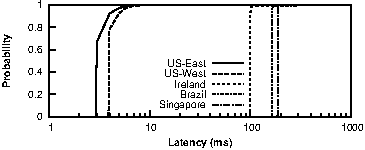
\includegraphics[width=0.65\columnwidth]{figures/redblue/thla2dcreadupdate.pdf}
\label{fig:microredup}
}
\hspace{2mm}
\subfloat[\textsf{\Red\ latency CDF for Singapore users as number of \dcs\ increases}]{
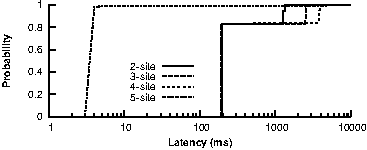
\includegraphics[width=0.65\columnwidth]{figures/redblue/thla2dcblueupdate.pdf}
\label{fig:microblueup}
}
\caption{\protect\subref{fig:microallredup} and \protect\subref{fig:microallblueup} show the average latency and standard
    deviation for \blue\ and \red\ requests issued by users in
    different locales as the number of \dcs\ is increased,
    respectively. \protect\subref{fig:microredup} and \protect\subref{fig:microblueup} show the CDF of latencies for \blue\ and
    \red\ requests issued by users in Singapore as the number of
    \dcs\ is increased, respectively.}
\label{fig:microuserbargraph}
\end{figure}

\if 0
In our microbenchmark application \changebars{users issue \operations\
 that touch a single randomly chosen object}  {we issue transactions with a single read
  or write request} in an open loop, i.e., each user has a window of
 outstanding \transactions. \changebars{Each \operation\
  is mapped to one shadow
  \transaction.  For simplicity, we label the original operations \red\ or \blue\ as well, according to the
color of their \shadow\ \operations. }{}The benchmark code allows for setting
  knobs with the ratio of read-only versus write-only \operations, and
 \blue\ versus \red\ \operations.

The dataset we used contains 10 tables\changebars{, each of which has
  the same schema consisting of 4 integer and 1 text attributes and is
  initialized with $100,000$ records. %, resulting in a $1.0$ GB
  dataset size.  }{, each of which with $100,000$ records.} The total
size of the dataset is $1.0$ GB. \changebars{}{Unless otherwise noted
  the workload does not contain any read-only requests.}
%for analysis after warm-up.}{}
%\daniel{remove the workload note and add a short note in every experiment that makes the flow more smooth}
}
\fi

\subsubsection{User observed latency}
The primary benefit of using \gemini\ to replicate a service across
multiple \dcs\ is the decrease in latency from avoiding the intercontinental round-trips as much as possible. As
a result, we first explore the impact of \RBc\ on user experienced
latency. In the following experiments each user issues a single
outstanding request at one time.
%Figure~\ref{fig:microuserbargraph} displays the average
%latency for users located in each of the five \changebars{\dcs}{data
%  centers}. 



%\changebars{In this experiment, the workloads consist of all write-only \transactions.}{}

%% \begin{figure}[t]
%% \centering
%% \subfigure[\red\ \transaction]{
%% \conferenceOnly{\includegraphics[width=0.95\columnwidth]{figures/redallUserBar.pdf}}
%% \techReportOnly{\includegraphics[width=0.7\columnwidth]{figures/redallUserBar.pdf}}
%% \label{fig:microallredup}
%% }
%% \subfigure[\blue\ \transaction]{
%% \conferenceOnly{\includegraphics[width=0.95\columnwidth]{figures/blueallUserBar.pdf}}
%% \techReportOnly{\includegraphics[width=0.7\columnwidth]{figures/blueallUserBar.pdf}}
%% \label{fig:microallblueup}
%% }
%% \caption{\changebars{Microbenchmark: + 0.1GB database}{} average latency of \blue\ and \red\ \transactions\ for users at different \dcs\ as the number of \dcs\ that replicate the service increases.}
%% \label{fig:microuserbargraph}
%% \end{figure}

Figure~\ref{fig:microuserbargraph}\subref{fig:microallredup} shows that the average
  latency for \blue\ requests is dominated by the latency between the
  user and the closest site; as expected, average latency decreases as
  additional sites appear close to the user. For example, with replicas in two sites in US, 
  users at US-East get responses in less than 10 ms, whereas users at 
  Ireland get responses of 100 ms on average, slightly above the round-trip latency of 92 ms presented
  in Table~\ref{tab:roundtriplatency}.
  Figure~\ref{fig:microuserbargraph}\subref{fig:microallblueup} shows that this trend 
  also holds for \red\ requests. The average latency and standard deviation,
  however, are higher for \red\ requests\ than for \blue\ requests. This
is because \red\ \shadow\ \operations\ can be as fast as \blue\ ones if
their primary site holds the unique red token, but will be much slower if
the site does not have that privilege.
  
Figures~\ref{fig:microuserbargraph}\subref{fig:microredup} and~\ref{fig:microuserbargraph}\subref{fig:microblueup} show the CDFs
  of observed latencies for \blue\ and \red\ requests, respectively,
  from the perspective of users located in Singapore.  The observed
  latency for \blue\ requests tracks closely with the round-trip
  latency to the closest \dc.  In the $k=2$ through $k=4$ \dc\ configurations,
  four \red\ requests from a user in Singapore are processed at the
  closest site during the one second in which the closest site holds
  the \red\ token; every fifth request must wait $k-1$ seconds for
  the token to return.  In the 5 \dc\ configuration, the local
  \dc\ also becomes a replica of the service and therefore
  a much larger number of requests (more than 300) can be processed
  while the local \dc\ holds the \red\ token.
  This changes the format of the curve, even though the
request issued immediately after the \red\ token is
released also needs to wait four seconds for the token to return.

\if 0
\changebars{
 Figure~\ref{fig:microallredup} shows that user perceived latency for
 an all \blue\ workload is dominated by the latency between the user
 and the closest site.  As expected, user perceived latency drops as
 additional sites are added to the system.  }
%old
{
\changebars{Regarding \blue\ \transactions\ , we notice that local
  users perceive a very low latency while for remote users the latency
  is dominated by the intercontinental round-trip. For example, as
  shown Figure~\ref{fig:microuserbargraph}\subref{fig:microallredup},
  with replicas in two sites in US, users at US-East get responses in
  less than 10 ms, whereas users at Ireland get responses of 100 ms in
  average, slightly above than the round-trip latency 92 ms presented
  in Table~\ref{tab:roundtriplatency}. As expected, the latency drops
  as we add more replicas to sites closer to the users.}{For
  \blue\ transactions, we observe that local users observe a very low
  latency due to close physical proximity, while the latency of remote
  users is dominated by the intercontinental round-trip. For example,
  as shown in
  Figure~\ref{fig:microuserbargraph}\subref{fig:microallredup}, with
  two data centers, users at US-East get responses from their local
  servers in less than 10 ms, while users at Ireland observe an
  average latency of 100 ms, slightly above than the round-trip
  latency 92 ms presented in Table~\ref{tab:roundtriplatency}. As
  expected, using more data centers improves user latency in some of
  the sites}.
}
%mtadone

%metanew
\changebars{}
%metaold
{
%new
\changebars{ Figure~\ref{fig:microallblueup} shows that the user
  perceived latency for an all \red\ workload is again dependent on
  the latency between the user and the closest service site, though
  the average and standard deviation are both higher than in the all
  \blue\ workload.  Both increases are driven by the time spent waiting
  for the \red\ token to return to the closest site. 
  %\MB{This is very difficult to explain and isn't clear; old text is/was dense and non-intuitive}
}
%old
{\changebars{Looking at \red\ \transactions\ in
    Figure~\ref{fig:microuserbargraph}\subref{fig:microallblueup} we
    still observe the general trend of latency improving as we
    increase the number of sites that replicate the service. However,
    there are two relevant differences between \blue\ and
    \red\ \transactions\ . First, the average latency for
    \red\ \transactions\ is higher, due to coordination across
    sites. Second, the standard deviation of the latency of
    \red\ \transaction increases as a result of using the
    \red\ token passing protocol for coordination. The results also
    show an unexpected low latency when compared to the average time
    that is required to wait for the coordination token. This is
    because the clients that issue \red\ transactions quickly fill up
    a window of pending requests while waiting for the token, but
    manage to issue many more requests when holding the token,
    therefore driving down the average latency. This effect is
    highlighted in the next set of
    graphs.}{Figure~\ref{fig:microuserbargraph}\subref{fig:microallblueup}
    shows the latency of \red\ transactions. While we still observe
    the general trend of latency improving as the number of sites that
    replicate the \changebars{service}{state} increases, there are two
    relevant differences between \blue\ and \red\ transactions. First,
    the average latency for \red\ transactions is higher, due to the
    need \changebars{of coordination}{to coordination} across sites in
    the form of passing around the \red\ token. Second, the standard
    deviation of the latency of \red\ transaction increases due to
    the same cause. The results also show an unexpectedly low latency
    when compared to the average time that is required to wait for the
    coordination token. This is because the clients that issue
    \red\ transactions quickly fill up a window of pending requests
    while waiting for the token, but manage to issue many more
    requests when holding the token, therefore driving down the
    average latency. This effect is highlighted in the next set of
    graphs.}  }
%done
}
%metadone
\fi

\subsubsection{Peak throughput}
We now shift our attention to the throughput implications
  of \RBc.  Figure~\ref{fig:micro2dcoverall1} shows a
  throughput-latency graph for a 2 \dc\ configuration and three
  workloads: 100\% \blue, 100\% \red, and a 70\% \blue/30\% \red\ mix.
  The different points in each curve are obtained by increasing the offered
  workload, which is achieved by increasing the number of
  outstanding requests per user.  
  For the mixed workload, users are partitioned into \blue\ and
  \red\ sets responsible for issuing requests of the specified color
and the ratio is a result of this configuration.

  The results in Figure~\ref{fig:micro2dcoverall1} show that increasing the
  ratio of \red\ requests degrades both latency and throughput.
In particular, the two-fold increase in throughput for the all \blue\ workload in
 comparison to the all \red\ workload is a direct consequence of the
 coordination (not) required to process \red\ (\blue) requests:
% Recall that \gemini\ enforces the total order of 
while \red\ requests can only be executed by
the site holding the \red\ token to process,
every site may independently process
 \blue\ requests.  The peak throughput of the mixed workload is
 proportionally situated between the two pure workloads.

\if 0
%old
{Next we looked at the impact of varying the
\blue\ \shadow\ \transaction\ ratio on system performance, by
measuring the \changebars{latency and throughput for write-only
  \shadow\ \transactions\ in a 2-sites deployment while we increase
  the user load. We ran three workload configurations: $100\%$ \blue,
  $100\%$ \red\ and a mix of \blue\ and
  \red\ \shadow\ \transactions\ where we split the users into two
  sets, each one responsible for issuing only one operation type,
  resulting in $70\%/30\%$ \blue/\red\ ratio. The results are shown in
  Figure~\ref{fig:micro2dcoverall} where the points in the curves
  corresponds sequentially to the same user load. We observe that
  increasing the fraction of \red\ \shadow\ \transactions\ degrades
  both latency and throughput.} {\transaction\ latency and throughput
  in a 2-data center deployment when running workloads with $100\%$
  \blue\ update transactions, $30\%$ \red\ update transactions, and
  $100\%$ \red\ update transactions. (The choice of $30\%$ was
  constrained by the fact that we wanted to split the users into two
  sets that only performed \blue\ and \red\ transactions,
  respectively, to avoid interference between the two types). The
  results in Figure~\ref{fig:micro2dcoverall} show that increasing the
  fraction of \red\ transactions degrades both latency and
  throughput. }
}
%done
\fi

%% \begin{figure}[t]
%%   \centering
%%     \conferenceOnly{\includegraphics[width=0.95\columnwidth]{figures/thla2dcredblue.pdf}}
%%     \techReportOnly{\includegraphics[width=0.7\columnwidth]{figures/thla2dcredblue.pdf}}
%%   \caption{ \changebars{Microbenchmark + 0.1GB database: throughput vs. latency graph with workloads of $100\%$ \blue, $100\%$ \red, and the mix of $70\%$ \blue\ and $30\%$ \red\ \transactions\ in a two-\dc\  setup.}{Throughput versus latency graph for the microbenchmark workload spanning two data centers when running a mix of: $100\%$ \blue, $30\%$ \red, and $100\%$ \red.} }
%%  \label{fig:micro2dcoverall}
%% \end{figure}

\begin{figure}[t]
  \centering
\includegraphics[width=0.85\columnwidth]{figures/redblue/thla2dcredblue.pdf}
  \caption{ Throughput versus latency graph for a 2 \dc\ configuration with
    varying \red-\blue\ workload mixes.}
%\changebars{Microbenchmark + 1.0GB database: throughput vs. latency graph with workloads of $100\%$ \blue, $100\%$ \red, and the mix of $70\%$ \blue\ and $30\%$ \red\ \transactions\ in a two-\dc\  setup.}{Throughput versus latency graph for the microbenchmark workload spanning two data centers when running a mix of: $100\%$ \blue, $30\%$ \red, and $100\%$ \red.} }
 \label{fig:micro2dcoverall1}
\end{figure}

\if 0
The degraded performance of the all \red\ workload is explained by
the need for cross-site coordination. In particular, in our
serialization protocol, at each point in time there is only one
\dc\ processing \red\ \transactions; the remaining ones are waiting
for the token, resulting in lower throughput and higher
latency. Introducing a mix of \blue\ \changebars{and
  \red\ \transactions}{transactions} sites run concurrent \dcs\ to
process transactions of one or both types at each moment, thus
increasing throughput. Moving to an \blue\ workload leads to a further
improvement in latency due to the possibility of executing
\transactions\ immediately without coordination. This highlights our
main motivation of running as many \blue\ \transactions\ as possible,
provided it does not undermine consistency.
\fi 

%metanew dropping scaling with datacenters
\if 0
\changebars{}
%metaold
{
%new
\changebars{Figure~\ref{fig:microScaleOverall} shows the
  throughput-latency curves for 2-5 \dc\ configurations processing a
  70 \blue/30 \red\ mixed workload.  We observe that both throughput
  and average latency improve as additional \dcs\ are added.  The
  latency improvement is the natural consequence of reducing the
  average distance between users and datacenters.  The throughput
  improvement is driven by the ability of \dcs\ to independently
  process \blue\ requests.
}{\subsubsection{Scalability with the number of sites}
}}
%metadone

%new dropping figure on scalability
\changebars{}
%old
{
\begin{figure}[t]
  \centering
  \conferenceOnly{\includegraphics[width=0.95\columnwidth]{figures/thla2dc3dc4dc5dcreadwrite.pdf}}
  \techReportOnly{\includegraphics[width=0.7\columnwidth]{figures/thla2dc3dc4dc5dcreadwrite.pdf}}
  \caption{\changebars{Microbenchmark:}{Microbenchmark} throughput
    vs.\ latency curves while varying the geo-replication factor from
    2 to 5 \dcs. }
 \label{fig:microScaleOverall}
\end{figure}
}
%done

%metanew
\changebars{

}
%metaold
{
To evaluate the scalability of \gemini\ with the number of geographic
locations of data, we deployed \gemini\ across 2 to 5 data centers and
measured both throughput and latency. In this experiment we fix the
mix of read/write and \blue/\red\ \changebars{\transactions}{} in a
balanced way that conservatively reflects our experience with
\changebars{the case studies}{real applications}, to 50/50 and 90/10,
respectively.

In Figure~\ref{fig:microScaleOverall} we plot the throughput and
latency for the four deployments. The different points in the same
curve correspond to a varying client load, which generates a higher
throughput but slower access times as the system saturates
\daniel{define it more precisely: how it varies?}. \changebars{These
  results unveils a trend, showing that \gemini\ scales well as the
  number of data-centers increases. Furthermore, despite the main
  benefit of \gemini\ be in latency, we can also observe a substantial
  improvement in system throughput following the same trend}{The
  results show that the performance of our architecture scales well as
  the number of data centers increases. Furthermore, despite the main
  benefit of \gemini\ being transaction latency, we can also
  substantially improve system throughput as the geo-replication
  factor increases,} due to two main reasons.  
%new
\changebars{The first reason is a direct consequence of latency
  improvement: as we add more data-centers close to users we amortize
  latency time in all transactions, therefore the transactions run
  faster and we end up with more transactions in the same experiment
  period. Second, we can also observe a shift in saturation wall, that
  is explained by the fact that we increase the capacity of the system
  as we add more data-centers to process users requests, enabling more
  local transactions (read-only) to be executed before the saturation
  point}
%old
{First, read-only transactions do not need to be propagated to
  remote sites. Second, it is cheaper for a data-center to process the
  shadow \transaction required for remote execution than to perform
  both the initial and the shadow transaction.}
%done
\daniel{the explanation is broken because microbenchmark read-only
  transactions were not being propagated before add more data-centers
  hence it did not change therefore cannot be the reason to improve
  the throughput specially when the system is not saturated. The
  second one is also broken because we already split the work of
  executing initial/generator transactions among more instances of
  proxies and the system is not saturated}
}
%metadone
\fi

\subsection{Case studies:  TPC-W and RUBiS}
Our microbenchmark experiments indicate that \RBc\ instantiated with
\gemini\ offers latency and throughput benefits in geo-replicated
systems with sufficient \blue\ \shadow\ \operations. Next, we evaluate \gemini\ using TPC-W and RUBiS.

\subsubsection{Configuration and  workloads}
In all case study experiments a single \dc\ configuration
corresponds to the original unmodified code with users distributed
amongst all five sites.  Two through five \dc\ configurations
correspond to the modified \RBct\ systems running on top of \gemini.
When necessary, we modified the provided user emulators so that each
user maintains $k$ outstanding requests and issues the next request as
soon as a response is received.

\paragraph{TPC-W.}
TPC-W~\cite{TPC-Wv18} defines three workload mixes
differentiated by the percentage of client requests related to making
purchases: browsing (5\%), shopping (20\%), ordering (50\%). The
dataset is generated with the following TPC-W
parameters: 50 EBS and $10,000$ items.  

%We specifically highlight the performance of the doBuyConfirm,
%discussed in detail in \S~\ref{sect:casetpcw}, and doCart, which adds
%items to and removes items from a specific shopping cart, requests.
%doCart always maps to a \red\ \shadow\ \operation. doBuyConfirm can
%map to either a \blue\ or \red\ \shadow\ \operation; in our
%experiments it is \red\ 98\% of the time.

\paragraph{RUBiS.}
RUBiS defines two workload mixes: browsing, exclusively comprised of
read-only interactions, and bidding, where $15\%$ of user
interactions are updates. We evaluate only the bidding mix. The RUBiS
database contains $33,000$ items for sale, 1 million users, $500,000$
old items and is $2.1$ GB in total.

%We specifically highlight the performance of StoreBid, which places a
%bid on an item, and StoreBuyNow, which purchases an item for the
%buyout price.  StoreBid always maps to a \blue\ \shadow\ \operation.
%StoreBuyNow may map to either a \blue\ or \red\ \shadow\ \operation;
%in our experiments it is \red\ 99\% of the time.

\subsubsection{Prevalence of \blue\ and \red\ \shadow\ \operations}

\begin{table}[t]
\centering
\begin{tabular}{|l||c|c||c|c|}
\hline
& {\Blue\  } &  {\Red\ } & read-only  & update\\
\hline
\hline
TPC-W shop&  99.2 & 0.8 &85 & 15\\
\hline
TPC-W browse &  99.5 & 0.5 & 96 & 4 \\
\hline
TPC-W order & 93.6  & 6.4 & 63 & 37 \\
\hline
RUBiS bid & 97.4 & 2.6 & 85 & 15\\
\hline
\end{tabular}
\caption{Proportion of \blue\ and \red\ \shadow\ \transactions\ and
  read-only and update requests in TPC-W and RUBiS workloads at
  runtime.}
\label{tab:mix}
\end{table}


Table~\ref{tab:mix} shows the distribution of \blue\ and
\red\ \shadow\ \operations\ during the execution of the TPC-W and RUBiS
workloads.  The results show that TPC-W and RUBiS exhibit sufficient
\blue\ \shadow\ \operations\ for it to be likely that we can exploit
the potential of \RBc.
%for \RBc\ to be a promising technique for
%building systems that are fast as possible and consistent when
%necessary.

\begin{figure}[H]
\centering
\subfloat[\textsf{TPC-W doCart}]{
\includegraphics[width=0.65\columnwidth]{figures/redblue/doCart/doCartallUserBar.pdf}
\label{fig:tpcwdocart}
}
\hspace{2mm}
\subfloat[\textsf{TPC-W doBuyConfirm}]{
\includegraphics[width=0.65\columnwidth]{figures/redblue/doBuyConfirm/doBuyConfirmallUserBar.pdf}
\label{fig:tpcwdobuyconfirm}
}
\\
\subfloat[\textsf{RUBiS StoreBid}]{
\includegraphics[width=0.65\columnwidth]{figures/redblue/storeBidallUserBar.pdf}
\label{fig:rubisStoreBid}
}
\hspace{2mm}
\subfloat[\textsf{RUBiS StoreBuyNow}]{
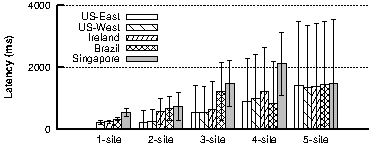
\includegraphics[width=0.65\columnwidth]{figures/redblue/storeBuyNowallUserBar.pdf}
\label{fig:rubisStoreBuyNow}
}
\caption{Average latency for selected TPC-W and RUBiS user
  interactions. \Shadow\ \operations\ for doCart and StoreBid are
  always \blue; for doBuyConfirm and StoreBuyNow they are \red\ 98\%
  and 99\% of the time respectively.}
\label{fig:tpcwrubisuserbargraph}
\end{figure}

\subsubsection{User observed latency}
We first explore the per request latency for a set of exemplar
\blue\ and \red\ requests from TPC-W and RUBiS.  For this round of experiments, each
\dc\ hosts a single user issuing one outstanding request to the
closest \dc.

From TPC-W we select doBuyConfirm (discussed in detail in
Section~\ref{ch:redblue:sect:casetpcw}) as an exemplar for \red\ requests and doCart
(responsible for adding/removing items to/from a shopping cart) as an
exemplar for \blue\ requests; from RUBiS we identify StoreBuyNow
(responsible for purchasing an item at the buyout price) as an
exemplar for \red\ requests and StoreBid (responsible for placing a
bid on an item) as an exemplar for \blue\ requests.  Note that
doBuyConfirm and StoreBid can produce either \red\ or
\blue\ \shadow\ \operations; in our experience they produce
\red\ \shadow\ \operations\ 98\% and 99\% of the time respectively.

Figures~\ref{fig:tpcwrubisuserbargraph}\subref{fig:tpcwdocart} and~\ref{fig:tpcwrubisuserbargraph}\subref{fig:rubisStoreBid} show
that the latency trends for \blue\ \shadow\ \operations\ are consistent
with the results from the microbenchmark---observed latency is directly
proportional to the latency to the closest \dc.  The raw latency
values are higher than the round-trip time from the user to the
nearest \dc\ because processing each request involves sending one or
more images to the user.
%; delivery time per image is one round-trip.

For \red\ requests, Figures~\ref{fig:tpcwrubisuserbargraph}\subref{fig:tpcwdobuyconfirm} 
and~\ref{fig:tpcwrubisuserbargraph}\subref{fig:rubisStoreBuyNow} show
that latency and standard deviation both
increase with the number of \dcs.  The increase in standard deviation
is an expected side effect of the simple scheme that \gemini\ uses to
exchange the \red\ token and is consistent with the microbenchmark
results.  Similarly, the increase in average latency is due to the
  fact that the time for a token rotation increases, together with the
  fact that \red\ requests are not frequent enough that several
  cannot be slipped in during the same token holding interval.  We
note that the token passing scheme used by \gemini\ is simple and
we leave as future work the implementation of a more sophisticated
scheme like Paxos~\cite{Lamport1998Paxos} for
regulating \red\ \shadow\ \operations.

\begin{figure*}[th!]
  \centering
\subfloat[\textsf{TPC-W shopping mix}]{
\includegraphics[width=0.88\columnwidth]{figures/redblue/thlatpcw1dc2dc3dc4dc5dc.pdf}
 \label{fig:tpcwoverall}
}
\\
\par\bigskip
\subfloat[\textsf{RUBiS bidding mix}]{
 \includegraphics[width=0.88\columnwidth]{figures/redblue/thla1dc2dc3dc4dc5dcRUBiSGemini.pdf}
  \label{fig:rubisoverall} 
}
\caption{Throughput versus latency for the TPC-W shopping mix and
  RUBiS bidding mix. The 1-dc line corresponds to the original code;
  the 2/3/4/5-dc lines correspond to the \RBct\ system variants.}
\label{fig:throughputscaling}
\end{figure*}

\subsubsection{Peak throughput}
We now shift our attention to the throughput afforded by our
\RBct\ versions of TPC-W and RUBiS, and how it scales with the
number of sites. For these experiments we vary the
workload by increasing the number of outstanding requests maintained by
each user.  Thr\-oughput is measured according to interactions per
second, a metric defined by TPC-W to correspond to user requests per
second.

Figure~\ref{fig:throughputscaling} shows throughput and latency for
the TPC-W shopping mix and RUBiS bidding mix as we vary the number of
\dcs.  In both systems, increasing the number of \dcs\ increases
peak throughput and decreases average latency.  The decreased latency
results from situating users closer to the \dc\ processing their
requests.  The increase in throughput is due to
processing \blue\ and read-only operations at multiple \dcs, given
that processing their side effects is relatively inexpensive.  The
speedup for a 5 \dc\ \gemini\ deployment of TPC-W is
3.7x against the original code for the shopping mix; the
5 \dc\ \gemini\ deployment of RUBiS shows a speedup of 2.3x.  


\begin{figure}[t!]
  \centering
\includegraphics[width=0.85\columnwidth]{figures/redblue/thla2dcTPCWallmixes.pdf}
  \caption{TPC-W: Throughput vs. latency graph for TPC-W with \gemini\ spanning two \dcs\ when running the three workload mixes. }
 \label{fig:tpcw2dcallmixes}
\end{figure}


Figure~\ref{fig:tpcw2dcallmixes} shows the throughput and latency
graph for a two \dc\ configuration running the TPC-W browsing,
shopping, and ordering mixes.  As expected, the browsing mix, which has
the highest percentage of \blue\ and read-only requests, exhibits the
highest peak throughput, and the ordering mix, with the lowest
percentage of \blue\ and read-only requests, exhibits the lowest peak
throughput. 
%For all workloads,
%\RBc\ improves latency by executing \operations\ closer to the user
%and improves throughput by not having to replicate all of the work,
%namely the execution of \initial\ \operations\ and
%read-only requests.

\subsection{Case study: Quoddy}
Quoddy differs from TPC-W and RUBiS in one crucial way: it has no
\red\ \shadow\ \operations.  We use Quod\-dy to show the full
power of \RedBlue\ geo-rep\-li\-ca\-tion.

Quoddy does not define a benchmark workload for testing purposes.  Thus we
design a social networking workload generator based on the measurement
study of Benevenuto et al.~\cite{Benevenuto2009Character}.  In this
workload, 85\% of the interactions are read-only page loads and 15\% of
the interactions include updates, e.g., request friendship, confirm
friendship, or update status.  Our test database contains 200,000
users and is 2.6 GB in total size.

In a departure from previous experiments, we run only two
configurations.  The first is the original Quoddy code in a
single \dc.  The second is our \gemini\ based \RBct\ version
replicated across 5 \dcs.  In both configurations, users are
distributed in all 5 regions.

Figure~\ref{fig:quoddyCDF} shows the CDF of user experienced latencies
for the addFriend operation. All \gemini\ users experience latency
comparable to the local users in the original Quoddy deployment; a
dramatic improvement for users not based in the US East region.  The
significantly higher latencies for remote regions are associated with
the images and javascripts that Quoddy distributes as part of processing the addFriend request.

\begin{figure}[t]
\centering
\includegraphics[width=0.85\columnwidth]{figures/redblue/thlaquoddyComparisonAll.pdf}
\caption{User latencies CDF for the addFriend request in single site Quoddy
   and 5-site \gemini\ deployments.}
\label{fig:quoddyCDF}
\end{figure}

                                                                                                                               

\subsection{\gemini\ overheads}


\gemini\ is a middleware layer that interposes between the
applications that leverage \RBc\ and a set of database systems where
data is stored. We evaluate the performance overhead imposed by our
prototype by comparing the performance of a single
\dc\ \gemini\ deployment with the unmodified TPC-W and RUBiS systems
directly accessing a database.
For this experiment we locate all users in the same \dc\ as the service.



\begin{table}[t]
\small
\centering
\begin{tabular}{|c|c|c|c|c|}
\hline
& \multicolumn{2}{c}{\textbf{TPC-W shopping}} & \multicolumn{2}{|c|}{\textbf{RUBiS biding}} \\
\cline{2-5}
& Original & Gemini & Original & Gemini\\
\hline
\hline
\specialcell{Thput. (inter/s)} &  409 & 386 & 450 & 370 \\
\hline
\specialcell{Avg. latency} & 14 ms & 15 ms & 6 ms & 7 ms \\
\hline
\end{tabular}
\caption{Performance comparison between the original code and the \gemini\ version for both TPC-W and RUBiS within a single site.}
\label{tab:performanceoverhead}
\end{table}

Table~\ref{tab:performanceoverhead} presents the peak throughput and
average latency for the TPC-W shopping and RUBiS bidding mixes. The peak
throughput of a single \dc\ \gemini\ deployment is between 82\% and 94\%
of the original and \gemini\ increases
latency by 1ms per request.  




%% \paragraph{Latency of individual requests.} 
%% To distinguish between the latency of \blue\ and \red\ transactions,
%% we separated the latency of two individual transactions of the system:
%% doCart (\blue) and \changebars{doBuyConfirmDecre}{doBuyConfirm}
%% (\red).  The results are shown in Figure~\ref{fig:tpcwuserbargraph}.

%% Similarly to the microbenchmarks, client latency for the \blue\ doCart
%% interaction (shown in Figure~\ref{fig:tpcwuserbargraph}\subref{fig:tpcwdocart}) decreases as
%% the latency to the closest replica decreases. We noticed, however,
%% that the latency observed by remote clients is a few times larger than
%% the round-trip latency between them and their nearest server. The
%% reason is that the doCart interaction performs the delivery of some
%% images (interspersed sequentially with transaction execution), and for
%% large images the effect of bandwidth differences between clients becomes
%% noticeable.

%% For the \red\ transaction that completes a purchase,
%% Figure~\ref{fig:tpcwuserbargraph}\subref{fig:tpcwdobuyconfirm} shows
%% that the transaction latency increases as the number of data centers
%% increases, with also an increase in the standard deviation. This is a
%% consequence of the fact that cross-site coordination gets more
%% expensive with the increase in the number of data centers,
%% particularly given that we employed a fixed timeout for passing the
%% coordination token between sites. In this case, since this
%% \red\ transaction occurs sporadically, it needs to wait on average
%% about half the token rotation period (or about 2 seconds for a five
%% site deployment).

%% \begin{figure}[t]
%%   \centering
%%   \conferenceOnly{\includegraphics[width=1.0\columnwidth]{figures/thla2dcTPCWallmixes.pdf}}
%%   \caption{TPC-W: Throughput vs. latency graph for TPC-W with \gemini\ spanning two \dcs\ when running the three workload mixes. }
%%  \label{fig:tpcw2dcallmixes}
%% \end{figure}



%% \paragraph{Overall benchmark performance.} In Figure~\ref{fig:tpcwoverall} we plot throughput vs.\ latency curves for the TPC-W benchmark. We plot five curves corresponding to deployments with replicas in one through five data centers. The results confirm that the system scales well with the number of geo-replication sites, reaching a maximum of 1500 interactions per second with replicas in five data centers, which is 3.67$x$ of the peak throughput achieved by running original TPC-W within a single site.



%% \begin{figure}[t]
%%   \centering
%%   \conferenceOnly{\includegraphics[width=1.0\columnwidth]{figures/thlatpcw1dc2dc3dc4dc5dc.pdf}}
%%   \techReportOnly{\includegraphics[width=0.75\columnwidth]{figures/thlatpcw1dc2dc3dc4dc5dc.pdf}}
%%   \caption{ \changebars{TPC-W: Throughput vs. latency graph of the
%%       original TPC-W in one data-center and TPC-W with
%%       \gemini\ spanning in 2 through 5 data-centers.}{Throughput and
%%       latency graph of the original TPC-W within one data center and
%%       TPC-W running on the top of \gemini\ systems and spanning 2
%%       through 5 datacenters.} }
%%  \label{fig:tpcwoverall}
%% \end{figure}

%% \subsubsection{RUBiS}
%% \label{sect:rubis}
%% RUBiS defines two workload mixes: a browsing mix consisting only of
%% read-only interactions and a bidding mix that includes $15\%$ of
%% updates. Our evaluation uses only the more general bidding mix. The
%% RUBiS database contains $33,000$ items for sale, 1 million users,
%% $500,000$ old items and is $2.1$ GB in total. For each experiment,
%% emulated clients continuously issue requests to the auction site, for
%% a time period of 10 minutes without think time.  We used the same
%% deployment conditions as in the TPC-W experiments.

%% \paragraph{Latency of individual transactions:} We report in
%% Figure~\ref{fig:rubisuserbargraph} the average latency observed by
%% users for two RUBiS interactions: \emph{storeBid} %
%% (Figure~\ref{fig:rubisuserbargraph}\subref{fig:rubisStoreBid}) and
%% \emph{storeBuyNow}.  %
%% (Figure~\ref{fig:rubisuserbargraph}\subref{fig:rubisStoreBuyNow}).
%% The \emph{storeBid} interaction contains a single \blue\ transaction
%% that puts a bid on an item, while the \emph{storeBuyNow}
%% interaction represents a more demanding operation, since it
%% includes a \red\ transaction that purchases items and updates the
%% stock.


%% As before, we observe significant latency benefits for
%% \blue\ transactions as we increase the number of data
%% centers. Furthermore, when interactions need to run a
%% \red\ transaction as in the case of {\tt storeBuyNow}, increasing
%% the number of data centers highlights the costs of cross-data
%% centers coordination. In this case the average latency of
%% \red\ transaction is slightly lower than in TPC-W because the
%% higher prevalence of \red\ transactions makes it more likely that
%% two or more \red\ transactions from the same sequence are executed
%% while holding the token (and thus the ones after the first one do
%% not wait).

% Additionally, we explore the impact of varying blue token timeout on the blue transaction latency. The outcome shows that shrinking the timeout improves the average latency of blue transactions.

%Similar to the TPC-W results, for the red interactions, using
%\gemini\ to replicate services across data centers will significantly
%improve the user observed latency. For example, moving from 2-data
%center to 5-data center, the \emph{storeBid} interaction latency
%observed by users at AG (Singapore) is dramatically changed from
%449.18 ms to 9.22 ms in average, and drops by $98.9\%$. Due to the
%blue token passing scheme, the average latency of \emph{storeBuyNow}
%observes a high standard deviation. Moreover, compared to the results
%of microbenchmark, the blue interaction average latency is much
%higher. The reason for this difference is that blue RUBiS
%interactions come into the system sparsely, while the blue
%microbenchmark interactions arrive intensively. Thus, the percentage
%of blue interactions for waiting in RUBiS is much higher than the one
%in microbenchmark. At the end, as we deployed RUBiS code in more data
%centers, the average latency of \emph{storeBuyNow} becomes larger,
%since the time of waiting for blue token gets longer.

%\rodrigo{I did not understand the following explanation: ``Moreover,
%compared to the results of microbenchmark, the blue interaction
%average latency is much higher. The reason for this difference is
%that blue RUBiS interactions come into the system sparsely, while the
%blue microbenchmark interactions arrive intensively. Thus, the
%percentage of blue interactions for waiting in RUBiS is much higher
%than the one in microbenchmark. At the end, as we deployed RUBiS code
%in more data centers, the average latency of \emph{storeBuyNow}
%becomes larger, since the time of waiting for blue token gets
%longer.''}

%\cheng{I want to explain why the average latency for blue
%transactions in RUBiS gets higher when the number the data centers
%increases, compared to the microbenchmark. The reason is that we have
%users in the microbenmark always issuing blue transactions in an open
%loop and the RUBiS doesn't. RUBiS selects blue transactions according
%to its probability table. Thus, there are fewer blue transactions in
%RUBiS than the microbenchmark. In addition, for the microbenmark,
%once the blue transaction is granted to a data center, its local blue
%users will issue a lot of blue transactions, which is more than the
%blue transactions that wait for the blue token. The majority fast
%blue transactions offset the delay introduced by the minority slow
%blue transactions. However, this doesn't hold in either RUBiS or
%TPC-W.}

%% \paragraph{Overall benchmark performance:} As shown in Figure~\ref{fig:rubisoverall}, the benchmark throughput scales well as we add geo-replication sites. In particular, the throughput scales from $450$ interactions per second in one site to $1,500$ interactions per second with five sites, an improvement of $233\%$.
%% % In addition to improve on latency provided to users, redblue consistency and \gemini\ are able to offer higher throughput. The latency and throughput graph for all deployment plans are shown in Figure~\ref{fig:rubisoverall}. The throughput of the three-site RUBiS with \gemini\ reaches 956 interactions per second and is $1.41x$ of the throughput of two-site. Remarkably, the throughput of the four-site RUBiS with \gemini\ is 1200 interactions per second and roughly $2x$ of the throughput of two-site. Moreover, the peak throughput of the five-site experiment is roughly 1500 interactions per section, which has been improved $123.9\%$, compared to the two-site one. 

%% \begin{figure}[t]
%% \centering
%% \conferenceOnly{\includegraphics[width=0.95\columnwidth]{figures/thla1dc2dc3dc4dc5dcRUBiSGemini.pdf}}
%% \techReportOnly{\includegraphics[width=0.7\columnwidth]{figures/thla1dc2dc3dc4dc5dcRUBiSGemini.pdf}}
%% \caption{Throughput vs.\ latency graph of the original RUBiS within one data center and RUBiS running on the top of \gemini\ spanning 2 through 5 data centers.}
%% \label{fig:rubisoverall}
%% \end{figure}

%% \subsection{Quoddy}
%% \daniel{we want to compare the best quoddy result with the the 5 dc
%%   setup. in this case, adding remote users to 1-dc will on increase
%%   the average latency and make original quoddy look bad. What we what
%%   to highlight that we are very close to quoddy best scenario, with
%%   the increased capacity and users across the globe in gemini
%%   scenario; therefore it is a fair comparison}

%% \paragraph{Quoddy.}
%% Quoddy does not define any benchmark workloads for testing purposes.
%% We design a social networking workload generator based on the
%% measrement study of Benevenuto et al.~\cite{Benevenuto09Character}.
%% In this workload 85\% of the interactions are read-only page loads and
%% 15\% of the interactions include updates, e.g., request friendship,
%% confirm friendship, or update status.  Our test database contains
%% 200,000 users and is 2.6 GB in total size.


%%  Unlike the two previous
%% case studies, the Quoddy social network does not come associated with
%% a benchmark specification that defines the application workload.
%% Therefore, we designed a workload generator for driving the user
%% behaviors.  The workload comprises of $85\%$ read-only interactions,
%% such as profile browsing actions and user searching, and $15\%$
%% read/write interactions including friendship requests/confirm and
%% status updates. These numbers are inspired on the results of a
%% measurement study of several social networking sites like Okurt,
%% MySpace and LinkedIn~\cite{Benevenuto09Character}.  The database
%% contains 200,000 users and is 2.6 GB in total. For each experiment,
%% the emulated users issue requests to the server for 10 minutes without
%% think time.

%% \begin{figure}[t]
%% \centering
%% \conferenceOnly{\includegraphics[width=0.95\columnwidth]{figures/thlaquoddyComparisonAll.pdf}}
%% \techReportOnly{\includegraphics[width=0.7\columnwidth]{figures/thlaquoddyComparisonAll.pdf}}
%% \caption{Distribution of latencies for addFriend interaction in Quoddy with the single site and
%% \gemini\ 5-site deployment.}
%% \label{fig:quoddyCDF}
%% \end{figure}

%% We only run Quoddy in a single data center and Quoddy with \gemini\ 
%% replicated across five data center experiments to examine the distribution 
%% of latency for different interactions. %\changebars{Unlike the deployment
%% %plans in TPC-W and RUBiS, the single data center Quoddy experiment only has local users,
%% %instead of additionally having remote users.}{Both deployment plans only have local users.} %We aggregate data from 
%% %users \changebars{}{at the five data centers}, and plot 
%% The latency CDF graph for the addFriend interaction is shown in Figure~\ref{fig:quoddyCDF}.
%% As can be seen, in the five data center case, 
%% all users observe almost the same latency as the one observed by local users at in the 
%% single data center experiment, even if Gemini servers are processing transactions 
%% received from other data centers also. The reason why Gemini impose no additional 
%% overhead is because all transactions encoded in interactions are \blue\ and thus processed locally.
%% The latency of the interaction is mostly due to the sequentially download of other resources, such as images.

%% %\rodrigo{Did not modify this paragraph, I think it's still in flux:}
%% %\cheng{Yes, we are working on this part.}
%% %Figure~\ref{} shows the throughput and latency numbers for Quoddy running on the top of \gemini\ and being replicated from 2 data centers to 5 data centers. As can be seen, the throughput has been improved significantly and the average latency has been reduced remarkably, as the number of data centers hosting service increases. In addition to the throughput and latency, we investigate evoluation of the user observed latency when we change the configuration from 2 data centers to 5 data centers. We find that the user observed latency is dramatically improved similarly to the red transactions presented in TPC-W and RUBiS. For example, users in Singapore observe xxx ms latency for read-info transactions in the two data center cases, and xxx ms latency in the five data center case. 

%% \subsection{Overhead of \gemini}


%% \gemini\ is implemented as a middleware layer that interposes between
%% the applications that leverage \RBc\ and a set of database systems
%% where data is stored. Next we evaluate the performance overhead that
%% is introduced by our system. For this, we compare the performance of a
%% single data center deployment of \gemini\ against a baseline
%% consisting of the applications directly accessing database via an unmodified JDBC driver.

%% %To support the redblue consistency model, we built a middle-tier (including coordinator, data writer and proxy library) to the traditional two-tier system architecture, in which application servers are connected to database directly via a JDBC driver. This new tier might lead to a performance drop. In order to understand how much overhead our new design introduces, we ran experiments of both the original code of two benchmarks and their redblue version with a single data center and local users.

%% %\begin{figure}[h!]
%% %\centering
%% %\subfigure[Throughput]{
%% %\includegraphics[width=0.45\columnwidth]{figures/overheadBar.pdf}
%% %\label{fig:thptOverhead}
%% %}
%% %\subfigure[Average latency]{
%% %\includegraphics[width=0.45\columnwidth]{figures/latencyOverheadBar.pdf}
%% %\label{fig:latencyOverhead}
%% %}
%% %\caption{Performance comparison between the original code and the \gemini\ version for both TPC-W and RUBiS within a single site.}
%% %\label{fig:overhead}
%% %\end{figure}

%% \begin{table}[t]
%% \small
%% \centering
%% \begin{tabular}{|c|c|c|c|c|}
%% \hline
%% & \multicolumn{2}{c}{\textbf{TPC-W}} & \multicolumn{2}{|c|}{\textbf{RUBiS}} \\
%% \cline{2-5}
%% & Original & Gemini & Original & Gemini\\
%% \hline
%% \hline
%% \specialcell{Thput. (inter/s)} &  409 & 386 & 450 & 370 \\
%% \hline
%% \specialcell{Avg. latency} & 14 ms & 15 ms & 6 ms & 7 ms \\
%% \hline
%% \end{tabular}
%% \caption{Performance comparison between the original code and the \gemini\ version for both TPC-W and RUBiS within a single site.}
%% \label{tab:performanceoverhead}
%% \end{table}

%% We compare both the peak throughput and average latency, and present
%% the results in Table~\ref{tab:performanceoverhead}.  \gemini\ achieves
%% $94.4\%$ and $82.2\%$ of the throughput of the original code, for
%% TPC-W and RUBiS respectively. In addition to this modest drop in
%% throughput, \gemini\ induces a latency that is, on average, 1 ms
%% higher per transaction when compared to the original benchmarks. This
%% shows that \gemini\ introduces modest overheads, likely worth the
%% performance benefits in geo-replicated deployments.

%%deployment of TPC-W and RUBiS is only 1 ms slower than the average latency of their original version. Although \gemini\ adds modest overhead to the original code with a single data center, it will make the original system more scalable by replicating it across multi-data centers.



%% %%%%%%%%%%%%%%%%%%%% round 2



%% \subsection{Application benchmarks (case studies)}
%% %Based on the results associated with the microbenchmark, we already saw the benefits gained when we use \gemini\ system to replicate data across multi-data centers. Next, we will show that \gemini\ also achieves good performance in the two application benchmarks: TPC-W and RUBiS.
%% Next we use our case studies to evaluate the system with application-level benchmarks.

%% \subsubsection{TPC-W}
%% \label{sect:tpcw}
%% TPC-W~\cite{TPC-Wv18} defines three workload mixes
%% differentiated by the percentage of client requests related to making
%% purchases: browsing (5\%), shopping (20\%), ordering (50\%). The
%% dataset is generated with the following TPC-W configuration
%% parameters: 50 EBS and $10,000$ items.  

%% For TPC-W experiments emulated clients issue requests for 10 minutes
%% with no think time.  We vary the offered workload by increasing the
%% number of outstanding requests maintained by each client.  One
%% \dc\ configurations correspond to the original TPC-W server with
%% clients in all regions; multiple \dc\ configurations use our
%% \RBct\ modifications and \gemini\ prototype.


%% \paragraph{Latency of individual transactions.}
%% We first 

%%  To distinguish between the latency of \blue\ and \red\ transactions, we separated the latency of two individual transactions of the system: doCart (\blue) and doBuyConfirm (\red).%\cheng{need to change, interaction is not red or blue, instead, transaction} 
%% The results are shown in Figure~\ref{fig:tpcwuserbargraph}.

%% % The main goal of \gemini\ is to offer low latency for users by allowing red transactions to be processed locally. In order to understand the evolution of user observed latency when the deployment plan changes, we further show in Figure~\ref{fig:tpcwuserbargraph} average latency for different interactions user observed at different data centers. Due to the space limitation, we only present two interactions: 

%% \begin{figure}[t]
%% \centering
%% \subfigure[doCart]{
%% \conferenceOnly{\includegraphics[width=0.95\columnwidth]{figures/doCart/doCartallUserBar.pdf}}
%% \techReportOnly{\includegraphics[width=0.7\columnwidth]{figures/doCart/doCartallUserBar.pdf}}
%% \label{fig:tpcwdocart}
%% }
%% \subfigure[doBuyConfirm]{
%% \conferenceOnly{\includegraphics[width=0.95\columnwidth]{figures/doBuyConfirm/doBuyConfirmallUserBar.pdf}}
%% \techReportOnly{\includegraphics[width=0.7\columnwidth]{figures/doBuyConfirm/doBuyConfirmallUserBar.pdf}}
%% \label{fig:tpcwdobuyconfirm}
%% }
%% \caption{Average latency for two system transactions: the doCart interaction shown in \subref{fig:tpcwdocart} is \blue, and the doBuyConfirm interaction shown in \subref{fig:tpcwdobuyconfirm} is \red.
%% %. \textbf{Note} that the first bar cluster represents a single-datacenter original version of TPC-W. The remaining four bar clusters refer to the redblue consistent version of TPC-W. The doCart interaction shown in \subref{fig:tpcwdocart} is red, and the buy confirm interaction shown in \subref{fig:tpcwdobuyconfirm} is blue.
%% }
%% \label{fig:tpcwuserbargraph}
%% \end{figure}

%% Similarly to the microbenchmarks, client latency for the \blue\ doCart
%% interaction (shown in Figure~\ref{fig:tpcwuserbargraph}\subref{fig:tpcwdocart}) decreases as
%% the latency to the closest replica decreases. We noticed, however,
%% that the latency observed by remote clients is a few times larger than
%% the round-trip latency between them and their nearest server. The
%% reason is that the doCart interaction performs the delivery of some
%% images (interspersed sequentially with transaction execution), and for
%% large images the effect of bandwidth differences between clients becomes
%% noticeable.


%% %% Starting to run the \RBct\ TPC-W with \gemini\, we were able to deploy it in multi-data centers. In the case study section, we know that the doCart interaction contains only \red\ transactions, so it can be processed locally without any global coordination. In the 2-dc case, we deployed servers in both UE and UW, so clients in UE and UW get low latency response. All other clients obtain almost the same latency as the 1-dc case, since they still remotely access to their data. In the 3-dc case, compared to the 2-dc case, we additionally deployed servers in EU. Consequently, the clients in EU obtain fast response. Once we deployed servers in every data center, we found that all clients get almost the same fast response. In addition to the ``shopping card'' interaction, the same evolution of latency has been found in all other interactions only containing \blue\ transactions. 

%% For the \red\ transaction that completes a purchase, Figure~\ref{fig:tpcwuserbargraph}\subref{fig:tpcwdobuyconfirm} shows that the transaction latency increases as the number of data centers increases, with also an increase in the standard deviation. This is a consequence of the fact that cross-site coordination gets more expensive with the increase in the number of data centers, particularly given that we employed a fixed timeout for passing the coordination token between sites. In this case, since this \red\ transaction occurs sporadically, it needs to wait on average about half the token rotation period (or about 2 seconds for a five site deployment).


%% %the user observed latency for an interaction ``doBuyConfirm'' involving a blue transaction. From 2-dc to 5-dc, as we keep increasing the number of data centers locating backend servers, we observed that the average latency for this interaction get higher. The reason for this increase is that the amount of time a data center spends waiting for getting blue token becomes longer when we have more data centers. In addition, we found that the average latency bar has a very high standard deviation. The deviation is also contributed by the blue token passing scheme. Once a data center holds the blue token, it can process blue transactions as fast as handling red transactions. As a result, there are some blue transactions completed in dozens of million seconds. However, if a data center is waiting for the blue token, all incoming blue transactions need to wait. These transactions will have a very high latency. For example, in 3-dc case, the maximum value can be up to 3 second.  

%% \paragraph{Overall benchmark performance.} In Figure~\ref{fig:tpcwoverall} we plot throughput vs.\ latency curves for the TPC-W benchmark. We plot five curves corresponding to deployments with replicas in one through five data centers. The results confirm that the system scales well with the number of geo-replication sites, reaching a maximum of $1.5k$ interactions per second with replicas in five data centers, which is $3.67x$ of the peak throughput achieved by running original TPC-W within a single site.
%% % The reasons for the throughput improvement are two aspects: a) read-only transactions are not propagated to remote sites; and b) applying shadow operations is cheaper than executing new transactions. In addition, the average latency dropped. The reason for the drop in latency is that more requests were processed locally when servers were placed closer to clients.
%% %In addition, we notice that the improvement in throughput of TPC-W is not as significant as the one of microbenchmark shown in Figure~\ref{fig:microScaleOverall}, when we scale it from 2-data centers to 5-data centers. The reason is that some read-only transactions contain complex queries. These complex queries are very computing-intensive and time-consuming. They are even heavier than read-write transactions.


%% \begin{figure}[t]
%%   \centering
%%     \conferenceOnly{\includegraphics[width=1.0\columnwidth]{figures/thlatpcw1dc2dc3dc4dc5dc.pdf}}
%%     \techReportOnly{\includegraphics[width=0.75\columnwidth]{figures/thlatpcw1dc2dc3dc4dc5dc.pdf}}
%%   \caption{Throughput and latency graph of the original TPC-W within one data center and TPC-W running on the top of \gemini\ systems and  spanning 2 through 5 datacenters.}
%%  \label{fig:tpcwoverall}
%% \end{figure}

%% \subsubsection{RUBiS}
%% \label{sect:rubis}
%% RUBiS defines two workload mixes: a browsing mix consisting only of read-only interactions and a bidding mix that includes $15\%$ of updates. Our evaluation uses only the more general bidding mix. The RUBiS database contains $33,000$ items for sale, 1 million users, $500,000$ old items and is $2.1$ GB in total. For each experiment, emulated clients continuously issue requests to the auction site, for a time period of 10 minutes without think time.  We used the same deployment conditions as in the TPC-W experiments.

%% \paragraph{Latency of individual transactions:} We report in Figure~\ref{fig:rubisuserbargraph} the average latency observed by users for two RUBiS interactions: \emph{storeBid}
%% % (Figure~\ref{fig:rubisuserbargraph}\subref{fig:rubisStoreBid}) 
%% and \emph{storeBuyNow}.
%% % (Figure~\ref{fig:rubisuserbargraph}\subref{fig:rubisStoreBuyNow}). 
%% The \emph{storeBid} interaction contains a single \blue\ transaction that puts a bid on an item, while the \emph{storeBuyNow} interaction represents a more demanding operation, since it includes a \red\ transaction that purchases items and updates the stock.  

%% \begin{figure}[t]
%% \centering
%% \subfigure[StoreBid]{
%% \conferenceOnly{\includegraphics[width=0.95\columnwidth]{figures/storeBidallUserBar.pdf}}
%% \techReportOnly{\includegraphics[width=0.7\columnwidth]{figures/storeBidallUserBar.pdf}}
%% \label{fig:rubisStoreBid}
%% }
%% \subfigure[StoreBuyNow]{
%% \conferenceOnly{\includegraphics[width=0.95\columnwidth]{figures/storeBuyNowallUserBar.pdf}}
%% \techReportOnly{\includegraphics[width=0.7\columnwidth]{figures/storeBuyNowallUserBar.pdf}}
%% \label{fig:rubisStoreBuyNow}
%% }
%% \caption{Average latency of two RUBiS interactions from all 5 datacenters. The storeBid interaction shown in \subref{fig:rubisStoreBid} contains only a \blue\ transaction, and the storeBuyNow interaction shown in \subref{fig:rubisStoreBuyNow} includes a \red\ transaction.}
%% \label{fig:rubisuserbargraph}
%% \end{figure}

%% As before, we observe significant latency benefits for \blue\ transactions as we increase the number of data centers. Furthermore, when interactions need to run a \red\ transaction as in the case of {\tt storeBuyNow}, increasing the number of data centers highlights the costs of cross-data centers coordination. In this case the average latency of \red\ transaction is slightly lower than in TPC-W because the higher prevalence of \red\ transactions makes it more likely that two or more \red\ transactions from the same sequence are executed while holding the token (and thus the ones after the first one do not wait).

%% % Additionally, we explore the impact of varying blue token timeout on the blue transaction latency. The outcome shows that shrinking the timeout improves the average latency of blue transactions.

%% %Similar to the TPC-W results, for the red interactions, using \gemini\ to replicate services across data centers will significantly improve the user observed latency. For example, moving from 2-data center to 5-data center, the \emph{storeBid} interaction latency observed by users at AG (Singapore) is dramatically changed from 449.18 ms to 9.22 ms in average, and drops by $98.9\%$. Due to the blue token passing scheme, the average latency of \emph{storeBuyNow} observes a high standard deviation. Moreover, compared to the results of microbenchmark, the blue interaction average latency is much higher. The reason for this difference is that blue RUBiS interactions come into the system sparsely, while the blue microbenchmark interactions arrive intensively. Thus, the percentage of blue interactions for waiting in RUBiS is much higher than the one in microbenchmark. At the end, as we deployed RUBiS code in more data centers, the average latency of \emph{storeBuyNow} becomes larger, since the time of waiting for blue token gets longer. 

%% %\rodrigo{I did not understand the following explanation: ``Moreover, compared to the results of microbenchmark, the blue interaction average latency is much higher. The reason for this difference is that blue RUBiS interactions come into the system sparsely, while the blue microbenchmark interactions arrive intensively. Thus, the percentage of blue interactions for waiting in RUBiS is much higher than the one in microbenchmark. At the end, as we deployed RUBiS code in more data centers, the average latency of \emph{storeBuyNow} becomes larger, since the time of waiting for blue token gets longer.''}

%% %\cheng{I want to explain why the average latency for blue transactions in RUBiS gets higher when the number the data centers increases, compared to the microbenchmark. The reason is that we have users in the microbenmark always issuing blue transactions in an open loop and the RUBiS doesn't. RUBiS selects blue transactions according to its probability table. Thus, there are fewer blue transactions in RUBiS than the microbenchmark. In addition, for the microbenmark, once the blue transaction is granted to a data center, its local blue users will issue a lot of blue transactions, which is more than the blue transactions that wait for the blue token. The majority fast blue transactions offset the delay introduced by the minority slow blue transactions. However, this doesn't hold in either RUBiS or TPC-W.}

%% \paragraph{Overall benchmark performance:} As shown in Figure~\ref{fig:rubisoverall}, the benchmark throughput scales well as we add geo-replication sites. In particular, the throughput scales from $450$ interactions per second in one site to $1,500$ interactions per second with five sites, an improvement of $233\%$.
%% % In addition to improve on latency provided to users, redblue consistency and \gemini\ are able to offer higher throughput. The latency and throughput graph for all deployment plans are shown in Figure~\ref{fig:rubisoverall}. The throughput of the three-site RUBiS with \gemini\ reaches 956 interactions per second and is $1.41x$ of the throughput of two-site. Remarkably, the throughput of the four-site RUBiS with \gemini\ is 1200 interactions per second and roughly $2x$ of the throughput of two-site. Moreover, the peak throughput of the five-site experiment is roughly 1500 interactions per section, which has been improved $123.9\%$, compared to the two-site one. 

%% \begin{figure}[t]
%% \centering
%% \conferenceOnly{\includegraphics[width=0.95\columnwidth]{figures/thla1dc2dc3dc4dc5dcRUBiSGemini.pdf}}
%% \techReportOnly{\includegraphics[width=0.7\columnwidth]{figures/thla1dc2dc3dc4dc5dcRUBiSGemini.pdf}}
%% \caption{Throughput vs.\ latency graph of the original RUBiS within one data center and RUBiS running on the top of \gemini\ spanning 2 through 5 data centers.}
%% \label{fig:rubisoverall}
%% \end{figure}

%% \subsubsection{Quoddy}
%% Unlike the two previous case studies, the Quoddy social network does not come associated 
%% with a benchmark specification that defines the application workload. 
%% Therefore, we designed a workload generator for driving the user behaviors. 
%% The workload comprises of $85\%$ read-only interactions, such as profile browsing actions 
%% and user searching, and $15\%$ read/write interactions including friendship requests/confirm 
%% and status updates. %These numbers are inspired on the results of a measurement study of several social networking sites like Okurt, MySpace and LinkedIn~\cite{Benevenuto09Character}. 
%% The database contains 200,000 users and is 2.6 GB in total. For each experiment, the emulated 
%% users issue requests to the server for 10 minutes without think time. 

%% \begin{figure}[t]
%% \centering
%% \conferenceOnly{\includegraphics[width=0.95\columnwidth]{figures/thlaquoddyComparisonAll.pdf}}
%% \techReportOnly{\includegraphics[width=0.7\columnwidth]{figures/thlaquoddyComparisonAll.pdf}}
%% \caption{Distribution of latencies in Quoddy for single site and
%% \gemini\ 5-site deployment.}
%% \label{fig:quoddyCDF}
%% \end{figure}

%% We only run Quoddy in a single data center and Quoddy with \gemini\ 
%% replicated across five data center experiments to examine the distribution 
%% of latency for different interactions. Both deployment plans only have local users. We aggregate data from 
%% users at the five data centers, and plot a latency CDF graph 
%% shown in Figure~\ref{fig:quoddyCDF}. As can be seen, in the five data center case, 
%% all users observe almost the same latency as the one observed by local users in the 
%% single data center experiment, even if Gemini servers are processing transactions 
%% received from other data centers also. The reason why Gemini impose no additional 
%% overhead is because all transactions encoded in interactions are \blue\ and thus processed locally.
%% The latency of the interaction is mostly due to the download of other resources, such as images.

%% %\rodrigo{Did not modify this paragraph, I think it's still in flux:}
%% %\cheng{Yes, we are working on this part.}
%% %Figure~\ref{} shows the throughput and latency numbers for Quoddy running on the top of \gemini\ and being replicated from 2 data centers to 5 data centers. As can be seen, the throughput has been improved significantly and the average latency has been reduced remarkably, as the number of data centers hosting service increases. In addition to the throughput and latency, we investigate evoluation of the user observed latency when we change the configuration from 2 data centers to 5 data centers. We find that the user observed latency is dramatically improved similarly to the red transactions presented in TPC-W and RUBiS. For example, users in Singapore observe xxx ms latency for read-info transactions in the two data center cases, and xxx ms latency in the five data center case. 

%% \subsection{Overhead of \gemini}


%% \gemini\ is implemented as a middleware layer that interposes between
%% the applications that leverage \RBc\ and a set of database systems
%% where data is stored. Next we evaluate the performance overhead that
%% is introduced by our system. For this, we compare the performance of a
%% single data center deployment of \gemini\ against a baseline
%% consisting of the applications directly accessing database via an unmodified JDBC driver.

%% %To support the redblue consistency model, we built a middle-tier (including coordinator, data writer and proxy library) to the traditional two-tier system architecture, in which application servers are connected to database directly via a JDBC driver. This new tier might lead to a performance drop. In order to understand how much overhead our new design introduces, we ran experiments of both the original code of two benchmarks and their redblue version with a single data center and local users.

%% %\begin{figure}[h!]
%% %\centering
%% %\subfigure[Throughput]{
%% %\includegraphics[width=0.45\columnwidth]{figures/overheadBar.pdf}
%% %\label{fig:thptOverhead}
%% %}
%% %\subfigure[Average latency]{
%% %\includegraphics[width=0.45\columnwidth]{figures/latencyOverheadBar.pdf}
%% %\label{fig:latencyOverhead}
%% %}
%% %\caption{Performance comparison between the original code and the \gemini\ version for both TPC-W and RUBiS within a single site.}
%% %\label{fig:overhead}
%% %\end{figure}

%% \begin{table}[t]
%% \small
%% \centering
%% \begin{tabular}{|c|c|c|c|c|}
%% \hline
%% & \multicolumn{2}{c}{\textbf{TPC-W}} & \multicolumn{2}{|c|}{\textbf{RUBiS}} \\
%% \cline{2-5}
%% & Original & Gemini & Original & Gemini\\
%% \hline
%% \hline
%% \specialcell{Thput. (inter/s)} &  409 & 386 & 450 & 370 \\
%% \hline
%% \specialcell{Avg. latency} & 14 ms & 15 ms & 6 ms & 7 ms \\
%% \hline
%% \end{tabular}
%% \caption{Performance comparison between the original code and the \gemini\ version for both TPC-W and RUBiS within a single site.}
%% \label{tab:performanceoverhead}
%% \end{table}

%% We compare both the peak throughput and average latency, and present the results in Table~\ref{tab:performanceoverhead}.  \gemini\ achieves $94.4\%$ and $82.2\%$ of the throughput of the original code, for TPC-W and RUBiS respectively. In addition to this modest drop in throughput, \gemini\ induces a latency that is, on average, 1 ms higher per transaction when compared to the original benchmarks. This shows that \gemini\ introduces modest overheads, likely worth the performance benefits in geo-replicated deployments.

%% %%deployment of TPC-W and RUBiS is only 1 ms slower than the average latency of their original version. Although \gemini\ adds modest overhead to the original code with a single data center, it will make the original system more scalable by replicating it across multi-data centers.


\section{Limitations and future work}
\label{ch:redblue:sect:limitation}
Although \RBc\ significantly succeeded at making our example applications fast, i.e.,
uniformly low user observed latency and high system throughput, without sacrificing
their targeted behavior, 
there are still several points, which we address in subsequent chapters.

First, \RBc\ offers a coarse-grained classification scheme, which can
lead to a conservative labeling result for applications that require
more consistency levels other than weak and strong consistency. We address this limitation by introducing
a generic consistency model providing us with more flexibility to express consistency requirements in Chapter~\ref{chapter:por}.

Second, the adoption of \RBc\ requires programmers to make effort to write shadow operations,
to apply changes to the original code,
and to reason about operation commutativity and invariant violation in
the presence of parallelism. Without the support of automatic tools, the 
manual work can be error-prone and does not scale, as
the code base increases. We address
this limitation by building SIEVE in Chapter~\ref{chapter:sieve},
which combines operational transformation and programming language techniques
to provide an automatic and provably correct solution.

Third, the simple token passing scheme for offering
strong consistency is not efficient and fault tolerant. At each point of time,
only one site can admit its \red\ \shadow\ \operations\ to the global
redblue order when this site is possessing
the \red\ token, while the remaining sites are waiting. This leads to a high latency
for user requests, and would cause the whole system to stop
executing this type of operations if the site where the red token stays crashes.
To address this limitation, we leave as future work
the implementation of Paxos for serializing all \red\ \shadow\ \operations\ across sites.

Fourth, using logical clocks might introduce false causal dependencies among
operations. As every site increases its own entry when assigning monotonic
timestamps to all its receiving operations, these operations become totally ordered, which,
provided that some of them are \blue, is not necessary. This might limit the 
amount of concurrency within a site, so we leave to future work
an analysis of the impact of the usage of logical clock on scalability.
%Despite the fact we believe that we have identified all
%relevant invariants in an easy way, we highlight that we could use
%tools for automatically inferring invariants to aid in this process
%~\cite{ErnstPGMPTX2007}.

\section{Summary}%\pagelimit{0.25}}
\label{ch:redblue:sect:conclusion}
In this chapter, we presented a principled approach to building
geo-replicated systems that are fast as possible and consistent when needed.
Our approach to addressing the
tension between running operations locally as often as possible
but without sacrificing important application properties, namely state
convergence and invariant preservation, hinges on
three major technical contributions:
1) a novel notion of \RBc\ allowing
both stron\-gly consistent (\red) \operations\ and causally consistent (\blue)
\operations\ to coexist, 2) a concept of \shadow\ \operation\ increasing the
coverage of \blue\ operations, and 3) a labeling methodology for
precisely determining which operations to be assigned which consistency level.
We implemented a distributed storage system called \gemini\ that 
execute and replicate \red\ and \blue\ \operations , and used it along with our labeling
conditions to run three existing web applications, namely TPC-W, RUBiS and Quoddy, under \RBCN.
Experimental results show that \RBc\ significantly improves the performance of geo-replicated
systems.



\chapter{Automatic consistency level assignment}
\label{chapter:sieve}
In this chapter, we describe the design, implementation and evaluation of \tool, the first tool to automate
the choice of consistency levels in a replicated system. \tool\ performs a combination of static and
dynamic analysis, offline and at runtime, to determine
when it is necessary to use strong consistency to preserve
these invariants and when it is safe to use causally consistent
commutative replicated data types (CRDTs).

This chapter is organized as follows. We first outline the motivation and contributions of \tool\ in Section~\ref{ch:sieve:sect:motivation}. Then
we discuss the most relevant related work in Section~\ref{ch:sieve:sect:related}. We present the design rationale of \tool,
and detail its implementation in Sections~\ref{ch:sieve:sect:overview},~\ref{ch:sieve:sect:commute},~\ref{ch:sieve:sec:label}. 
Section~\ref{ch:sieve:sect:evaluation} describes the case study applications, the experience on applying \tool\ to these applications, and the corresponding 
experimental results. Finally, we discuss \tool's limitations in Section~\ref{ch:sieve:sect:limitation} 
and conclude this chapter in Section~\ref{ch:sieve:sect:conclude}.

\section{Motivation and contributions}
\label{ch:sieve:sect:motivation}

As mentioned in Chapter~\ref{chapter:intro}, the providers of
planetary-scale services---such as Google~\cite{GoogleWeb}, Amazon~\cite{AmazonWeb}, or Facebook~\cite{FacebookWeb}
face an inherent tension between improving performance and maintaining targeted consistency
semantics. In order to resolve this tension, in Chapter~\ref{chapter:redblue}, we presented
the \RBCN\ framework, which offers the choice between executing an operation under a strong or a weak
consistency model, and the methodology for increasing the safe usage of weak consistency. 
As shown in Section~\ref{ch:redblue:sect:casestudies} in Chapter~\ref{chapter:redblue},
adapting existing applications to \RBCN\ consists of the following
two manual tasks. First, one must transform every application operation into a generator and a
set of commutative shadow operations, each of which corresponds to a distinct
side effect. Second, one must correctly
identify which shadow operations may break application invariants,
and label them appropriately so that they execute under strong consistency.
Although our experience shows that modifying benchmark applications
to be \RBCAJ\ is not difficult, in practice, as the code base increases, this manual work can 
become very challenging and error-prone. This is because it
imposes on the application programmer the non-trivial burden of
a) figuring out side-effects of every code path in the original operations;
b) implementing shadow operations and verifying whether any pair of them commutes; and c)
understanding the semantics of each shadow operation \changebars{to determine if they meet
the properties for safe execution under weak consistency.}{and how
the assignment of different consistency levels (either weak or strong consistency) to different shadow operations influences
overall semantics that are perceived by the users.} 

In this chapter, to ease this burden on the programmer,
we present \tool, the first tool (to the best of our knowledge) that automates
this adaptation to multi-level consistency such as \RBCN. This tool focuses on
an important and widely deployed class of applications, namely
Java-based applications with a database backend. Overall, we make the following contributions:

\begin{enumerate}
\item {\bf Commutativity transformation.} One of the obstacles for labeling a large number
of operations as \blue\ is the fact that not many operations are naturally
commuting with all others, as shown in Section~\ref{ch:redblue:sect:casestudies} in Chapter~\ref{chapter:redblue}. 
To ensure good performance, \tool\ automatically transforms the side effects of every application operation into their commutative
form. To this end, we build on previous work on commutative replicated data types
(CRDTs)~\cite{Shapiro2011Conflict,Preguica2009CRDT}, i.e., data types whose
concurrent operations commute, and apply this concept to relational
databases. This allows programmers to only specify which particular CRDT semantics they intend by
adding a small annotation in the database schema, and \tool\ automatically
generates the shadow operation code implementing the chosen semantics.
%In the absence of an annotation, \tool\ implements the default ``last writer
%wins'' semantics, whereby the write with the largest timestamp completely
%overwrites any earlier writes.

\item {\bf Efficient labeling.} \tool\ uses program analysis to identify commutative shadow operations that might
violate application-specific invariants when
executed under weak consistency semantics, and runs them under strong
consistency. To make the analysis accurate and lightweight,
we divide it into a potentially expensive static part and an
efficient check at runtime. The static analysis generates a set of
abstract forms ({\em templates}) that represent the space of possible shadow operations produced at runtime,
and identifies for each template a logical condition ({\em weakest precondition}) under which
invariants are guaranteed to be preserved. This information is
then stored in a dictionary, which is looked up and evaluated at
runtime,
% when a shadow operation is produced,
%we perform a quick lookup to retrieve the corresponding static logical condition,  and evaluate it
to determine whether each shadow operation can run under weak consistency.

\item {\bf Minimal manual intervention.} Unlike previous work, in which
either the adoption of new programming models or a significant number of changes to
the original source code is needed, using \tool, the programmer has to 
only specify the application invariants that must be preserved
and to annotate a small amount of semantic information
about how to merge concurrent updates, while keeping the application code base unchanged.
\end{enumerate}

%\begin{itemize}
%
%\item Since commutativity is required for the use of weak consistency,
%  \tool ensure that all operations commute by design.  To this end, we
%  propose a set of commutative replicated data types
%  (CRDTs)~\cite{Preguica2009CRDT}, i.e., data types whose operations
%  commute when they are concurrent, aimed at applications that store
%  their persistent state in a relational database. These CRDTs require
%  a small annotation in the database schema, only to disambiguate the
%  semantics of updates. With the support of CRDTs,
%  \tool\ automatically transforms the side effects of every
%  application operation into their commutative forms.
%
% \allen{Why is commutativity required for weak consistency?  we know
%   that, but I don't know where that knowledge comes from}
%
%\allen{``We propose a set of CRDTs'' makes it sound like the CRDTs are
%  a contribution of the work.  My understanding is that they are a
%  tool we are leveraging for commutativity.  Corollary: What are the
%  contributions that we want to emphasize?}
%
%\item We resort to program analysis to determine whether operations
%  can violate invariants when they are executed under weak
%  consistency. In particular, we split this analysis into a relatively
%  expensive static part and an efficient check at runtime. The static
%  analysis uses an automated verification tool called
%  Jahob~\cite{Kuncak2007Jahob} to identify a set of logical conditions
%  (weakest preconditions) of all execution patterns, under which
%  invariants are preserved. These static logical conditions are then
%  efficiently validated at runtime to determine whether operations can
%  run under weak consistency or not.
%
%\end{itemize}


%\allen{Taking a step back, the current intro does a good job of
%  enumerating the techniques used but does not clearly identify the
%  technical challenges we faced in implementing those techniques.
%  I.e., why is/was the dictionary hard to build?  One take on what
%  we've got so far is a clear identification of the problem space and
%  strategy we want to use; what is missing, in my opinion, is the
%  challenges that we have to overcome in order to implement our
%  strategy.}


% These are that weakly consistent operations must commute with all
% other operations, and that incorporating their side effects against a
% state that is different than the one that produced those side effects
% cannot lead to the violation of invariants

\if 0

\rodrigo{In terms of motivation, we shouldn't narrow the scope unnecessarily to
the problem of addressing the automatization of our RedBlue work. I
think we have a broad motivation which is to address a problem raised
in Doug Terry's talk ~\cite{Terry2011Baseball}, which is that of helping
applications determine what level of consistency they require, and
doing so at the finest possible granularity so that they can be fast
when possible and consistent if necessary.
Then, in terms of the solution, I would say that we are based on the
observation that there are two crucial properties involved in the
classification, which are commutativity and invariant-preservation
(need to explain what that means), and then we use two key ideas:
1. A careful separation between statically analyzing the conditions
under which operations preserve invariants, and a fast, dynamic check
to determine of the parameters fed to the operations meet those
conditions.
2. The use of CRDTs to build operations that commute by design,
precluding the need to analyze the code for commutativity.}

Geo-replication~\cite{Hamilton2008GeoFacebook, Cooper2008PNUTs, DeCandia2007Dynamo, 
Calder2011Azure, Corbett2012Spanner}, replicating data at geo-graphically dispersed data centers (sites), is
a major solution for popular online services to scale themselves to meet the
needs of their increasingly growing user base. With this technique, users
contact a nearby site to get fast responses, and coordination among
all data centers is required to keep data globally consistent. However, offering low latency
and maintaining strong consistency cannot be achieved simultaneously~\cite{Brewer2010CAP}, as
a result of the high cost of immediate inter-site coordination required by strong consistency. In order to
offer low latency, many geo-replicated systems~\cite{DeCandia2007Dynamo,Lloyd2011COPS} 
resort to use a weak consistency model that allows data to temporally diverged and guarantees
the final data convergence. 

One of the most popular weak consistency models is \emph{eventual consistency}~\cite{Vogels2008Eventual}, 
in which each site independently processes requests
without immediate coordination, updates are asynchronously exchanged across sites, and conflicts
are resolved at either storage system level or application level. Although eventual consistency
and its invariants have been widely deployed in many services, its
practical usage is still problematic, since some invariants or constraints that need to hold 
globally true may be violated. For example, the unacceptable state that the last book sold to
multiple distinct users appears in an eventually consistent online shopping cart application. 

To prevent applications from breaking their invariants, while preserving fast responses,
some recent work like Lazy Replication~\cite{Ladin1992LazyRep}, Geo-transaction ~\cite{Sovran2011TranGeo} and RedBlue
Consistency ~\cite{Li2012RedBlue} proposed to allow strong consistency to co-exist
with eventual consistency in a single system. This proposal achieves fast responses 
by running eventually consistent operations at any site, and ensures invariant preservation
by globally coordinating strongly consistent operations. Most recently, Terry
 et al. identified a six-level consistency model retaining the above two
and containing four new consistency semantics in between~\cite{Terry2013CBSLA}.

The key to adopting the hybrid consistency model for geo-replication is to
decide which part of a system can be eventually consistent and 
which part must be strongly consistent. A principled classification methodology,
presented by RedBlue Consistency~\cite{Li2012RedBlue}, associates 
eventual consistency with an operation if it commutes with all others 
and doesn't violate any invariant, and attaches strong consistency to the rest. 
With this solution, however, programmers have to manually prove operation commutativity and
invariant preservation. Moreover, in order to enable geo-replication to lead
to performance benefits, an application must have a majority of operations 
to be eventually consistent. However, in practice, not many operations are naturally
commuting with all others. RedBlue Consistency tried to address this problem by 
asking programmers to manually transform non-commutative
operations to be commutative. The significant drawback of these two
manual tasks is that they are not scalable and can be error-prone while
being applied to large-scale code base.

In this project, we aim at automatically constructing more commutative
operations for an application, and categorizing operations into
the strongly and eventually consistent groups. The key idea to achieving this goal
is to first make every operation commutative (can be eventually consistent), 
and then identify a set of commutative operations that potentially violate invariants
(must be strongly consistent).

We built an automatic tool, \tool, to instantiate the above key ideas. \tool\ relies on
two important techniques, namely, commutative replicated data types (CRDTs)~\cite{Preguica2009CRDT}
and Jahob~\cite{Kuncak2007Jahob}. CRDTs is a set of data types whose operations commute
when they are concurrent. With the support of CRDTs, \tool\ first transforms the side effects of every execution of application
transactions into their commutative forms (\emph{shadow operations}~\cite{Li2012RedBlue}). 
Due to the commutativity obtained by design, all shadow operations can be potentially 
labeled as eventual consistency. To enable this transformation, we still require 
developers to annotate their applications with a minimal amount of information to indicate which 
conflict merging solution they want to apply to a state or an operation. Unlike the previous
manual processes, the human intervention within our solution is much less. In addition, programmer 
supplied annotations can be automatically derived from an analysis over data manipulation patterns. 
We leave this as future work. 

Jahob is a verification tool to statically prove whether program properties are
satisfied in all possible executions. \tool\ uses Jahob to identify a set of logical 
conditions (weakest preconditions) of all execution patterns, under which invariants 
are preserved. These static logical conditions will be efficiently validated at runtime for
the shadow operation classification. A shadow operation must be strongly consistent 
if the weakest preconditions of its corresponding execution pattern are evaluated to \texttt{False} ;
Otherwise, it can be eventually consistent.

In addition, our tool \tool\ has the following properties: (a) \textbf{applicability} 
It is easy-of-use. Programmers who want to adopt this approach are only required to invest a minimal 
amount of time and effort; (b) \textbf{correctness} The transformation ensures state convergence, 
and the classification guarantees that no invariants are violated; 
(c) \textbf{scalability} It is scalable, despite that the complexity of application semantics 
and the number of application operations significantly increase; and (d) \textbf{incrementally} 
It is able to incrementally classify operations in the case when programs are changed. 
For example, if programmers change a small part of their code, this solution doesn't need to classify all 
operations again, instead only re-considers these modified operations and all relevant operations.

\fi
We evaluate \tool\ using TPC-W and RUBiS. Our results show that it
is possible to achieve the performance benefits of weakly consistent replication
when it does not lead to breaking
application invariants without imposing the burden of choosing
the appropriate consistency level on the programmer, and with
a low runtime overhead.


\section{Related work}
\label{ch:sieve:sect:related}
We summarize and compare previous work with \tool\ according to the
following categories:

\noindent\paragraph{Weak consistency and commutativity.} 
In order to provide users with low latency access to web services,
a wide range of their underlying replicated systems have relied on weak
consistency such as causal consistency. They produce a reply to the user
 as soon as the corresponding operation executes in a single replica 
with respect to physical proximity. The usage of these systems requires
a special care, i.e., they must be equipped with procedures for handling 
conflicts that may arise from concurrent operations. In some
systems, such as Bayou~\cite{Terry1995Managing},
Depot~\cite{Mahajan2010Depot}, and Dynamo \cite{Decandia2007Dynamo},
the programmer has to provide application-specific code for merging 
concurrent versions. Other systems, such as Cassandra~\cite{Lakshman2010Cassandra},
COPS~\cite{Lloyd2011Causal}, Eiger~\cite{Lloyd2013Stronger} and
ChainReaction \cite{Almeida2013Chainreaction}, use a simple
last-writer-wins strategy for merging concurrent versions. This
simple strategy may, however, lead to lost updates.
%, making it inappropriate for
%many applications.
%However, because they never use strong
%consistency, these systems cannot guarantee that invariants are
%preserved when two operations execute concurrently.

Some systems have explored using operation
commutativity to guarantee that all replicas converge to the same
state, regardless of operation execution order. For example, 
Pregui{\c c}a et al. and Shapiro et al. propose CRDTs (commutative or conflict-free replicated data types), 
a set of abstract data types whose operations commute in presence of
concurrency\cite{Preguica2009CRDT,Shapiro2011Conflict}.
Most recently, Walter \cite{Sovran2011PSI} includes a single pre-defined commutative data type, 
\emph{cset}, which could be seen as an appreciation of the previous CRDT work. 
Commutative operations that implement variants of
CRDTs can also be used in different frameworks such as Lazy replication \cite{Ladin1992LazyReplication},
RedBlue \cite{Li2012RedBlue}, Generalized-Paxos~\cite{Lamport2005GeneralizedPaxos}, and Generic-Broadcast~\cite{Pedone99genericbroadcast}, 
for supporting unordered execution of these operations and hence making
the corresponding systems or protocols more scalable.

The major drawback of these above systems is that operation commutativity is achieved
at a cost, i.e., by either modifying existing application code or adopting
a new programming model. Unlike these systems, 
\tool\ instead offers the programmer a CRDT library and automatically 
generates commutative shadow operations that encode side effects of every application operation at runtime, 
requiring only a small amount of CRDT annotations
specifying the merging semantics. This automation eases the burden on the programmer
and eliminate errors of implementing these semantics, from application to application.

%\allen{These papers do not logically make sense together.  CRDTs
%  discuss how to make operations commute; RBC discusses how to
%  coordinate sites and the order in which they can be applied.  I am
%  not sure what Geo-transaction does.  Note that COPS, Eiger,
%  transaction chaining, .... need to be included here as well.
%  Additionally, the commutativity work from MIT at SOSP this year
%  should be included.}
%  
%\nuno{commutativity work from MIT at SOSP has little to do with eventual
%consistency - we could say something like:
%Commutativity has also been explored in other settings for improving performance,
%such as operating systems \cite{Clements13Scalable}. 
%CRDTs \cite{Preguica2009CRDT,Shapiro11Conflict} extend solutions used in these
%works by providing commutative design for a large number of useful data types,
%including counters, set, maps, graphs.  }
%
%\allen{the connection between commutativity and scalability extends
%  beyond eventual consistency to performance in multicore
%  environments~\cite{Clements13Scalable}}
%  
% \nuno{I don't see how to integrate reference to this smoothly in the text...}

\noindent\paragraph{Classification for multi-level consistency.}
\tool\ is built on top of a two-level consistency model, in which
operations execute under either strong or weak consistency. The primary goal of 
\tool\ is to automatically assign appropriate consistency levels to various 
operations so that state convergence and invariant preservation are ensured despite 
having weakly consistent replication. The consistency level assignment problem has been
studied in many recent multi-level consistency proposals. For example,
relying on a probabilistic model, consistency
rationing~\cite{Kraska2009ConsisRation} associates different
consistency levels with different states, instead of operations, and
allows states to switch from one level to another at runtime. Unlike
this approach, we partition operations into strong and causal
consistency groups. Pileus is a replicated key-value store,
which trades off between consistency and latency requirements of read-only operations
via consistency-based service level agreements (SLAs)defined by the user~\cite{Terry2013SLA}. 
Different than Pileus, \tool\ does not restrict operation types. In addition,
both RedBlue consistency~\cite{Li2012RedBlue} 
and I-confluence~\cite{Bailis2014Avoid} define conditions that
operations must meet in order to run under weak consistency, i.e.,
without coordination. We build on this line of work and extend
it so that an automatic tool, and not the programmer, is responsible
for determining whether the operations meet these conditions.

\noindent\paragraph{Automation.}
To free programmers from manually making choices of consistency levels, 
some researchers have attempted to apply program
analysis techniques to reason about the consistency requirements
of real applications. Alvaro et al.~\cite{Alvaro2011Bloom, Alvaro2014Blazes} identify code locations
that need to inject coordination to ensure target consistency semantics, while Zhang
et al.~\cite{Zhang2013TransactionChain} inspect read/write conflicts 
across all operations. However, they merely focus on commutativity, and ignore application invariants, which
are very important and taken into account by our solution. Instead
of a fully static solution, we offer a dynamic and optimistic classification by combining a static analysis of 
computing weakest preconditions for shadow operations and a runtime evaluation
to determine operations to be strongly consistent if
the corresponding conditions evaluate to {\tt FALSE}. 

Very recently, the concept of warranties imposes a set of time-limited invariant-related assertions
over shared objects in a replicated system, and allows transactions
to commit without coordination if the relevant assertions
are still valid~\cite{Liu2014Warranties}. Compared with warranties, preconditions in \tool\ 
are logical formulas defined over parameters of shadow operations rather than system state. As a result,
\tool\ is able to always perform condition checks locally, while warranties have to 
invalidate assertions when updates are replicated or the expiration time reaches, and to delay updates 
for make read-only transactions fast. 
The work from Roy et al.~\cite{Roy2014Adaptive} resembles the concept of warranties and presents an
 algorithm to analyze transaction code for producing warranties. That work is complementary to the goal of \tool\ 
since we rely on a verification tool, Jahob~\cite{Kuncak2007Jahob}, to determine certain properties (encoded in
weakest preconditions) of shadow operations.

\noindent\paragraph{Other related work.} 
Commutativity has been explored in other settings to improve
performance and scalability -- e.g., in databases~\cite{Weihl1988Commutativity}
and in OS design for multi-core 
systems~\cite{Clements2013Scalable}.
Program analysis techniques have also been used to 
identify commuting code blocks. Aleen et
al.~\cite{Aleen2009CommuteAnalysis} propose a new approach to find
commutative functions automatically at compile time for allowing
legacy software to extract performance from many-core
architectures. Kim et al.~\cite{Kim2011CommuteVerification} used the
Jahob verification system to determine commuting conditions under
which two operations can execute in different orders. 
Unlike these two prior solutions that only focus on identifying commutative
code blocks, our tool automatically transforms operations
by decoupling side effect generation and application, which makes more 
operations commute~\cite{Li2012RedBlue}, and we also focus on determining
invariant safety.


%Unlike these two prior solutions, our tool automatically transforms operations to
%be commutative using a set of CRDTs, and consequently, all transformed
%operations are provably commutative and verification is no longer
%needed. Another remarkable difference between the two proposals and
%ours is that they identify commutativity as much as the code provides,
%however, our tool is able to make more operations commutative.

%\section{Background}
\label{ch:sieve:sect:background}

%In this section, we provide background on the techniques that our
%work builds upon.
Before presenting the various aspects of \tool, we first
introduce the system model it builds upon, and the operation classification 
methodology it relies on.

%\subsection{RedBlue consistency}
%\label{sect:backredblue}

In previous work~\cite{Li2012RedBlue}, we defined RedBlue
consistency, where operations can be labeled red (strongly consistent)
or blue (weakly consistent). Red operations are totally ordered with
respect to each other, meaning that they execute in the same relative
order at all replicas, and therefore no two red operations execute
concurrently. (This corresponds to the requirements of serializability.)
 In contrast, blue operations can be reordered with
respect to other operations, provided they preserve causality
(corresponding to causal consistency).

A pre-requisite to being able to label operations as blue is
that operations should commute, so that executing them in a different
order at various replicas does not lead to a divergent replica state.
To increase the space of commutative operations, we proposed a change in the state machine replication model such that
operations are split between a generator operation running only on the
replica that first receives the operation and producing no side
effects, and a shadow operation sent to all replicas, which effectively applies the
side effects in a commutative way. More formally, in the original state
machine replication model, an operation $u$
deterministically modifies the state of a replica from $S$ to $S'$
(denoted as $S+u=S'$). In the proposed model, the application
programmer decomposes every operation $u$ into generator and shadow
operations $g_u$ and $h_u(S)$, respectively, where $S$ is the replica state
against which $g_u$ was executed. The pair of generator and shadow operations
must satisfy the
%Furthermore, there is the
following correctness requirement: for any state $S$, $S+g_u = S$ and $S+h_u(S) = S+u$.

Given this system model, we defined sufficient
conditions for labeling operations in a way that ensures that
application invariants are not violated.
In particular, a shadow operation can be labeled blue if
it commutes with all other shadow operations, and it is {\em invariant
safe}, 
%meaning that for all states $S$ and $S'$ that preserve the
%invariants, the state $S'+h_u(S)$ also does so.
meaning that if states $S$ and $S'$ preserve the
invariants, then the state $S'+h_u(S)$ does so as well.

%\subsection{Commutative replicated data types}

%Commutative replicated data types (CRDTs)~\cite{Shapiro11Conflict,Preguica2009CRDT} are  data types
%whose operations commute, allowing state to converge
%irrespectively of the order by which a given set of
%operations is executed. There already exist a series of systems and libraries
%that implement CRDTs for the most relevant data types, such as sets,
%counters, strings, etc. Programmers can leverage CRDTs by modifying
%their code to store all state using these data types. 


\if 0

In this section, we basically iteratively present the fundamental
techniques that we built our tool on the top of. For example,
commutative replicated data types, shadow operation, weakest
precondition. Perhaps we also can add something like system model.

\allen{What is the point of this section?  Reading it now, it touches
  on technique-key words that are, by-and-large, meaningless to me
  because I don't understand the context for why they are being
  brought up.  Is this supposed to be a system model section that
  makes explicit the technical challenges that induce our results?  or
  what?}

\subsection{System model}
In our context, every geo-replicated service fully replicates its data across multiple sites. 
Each site runs the same configuration consisting of a persistent storage
system, a set of application proxy servers, and a coordinator. Communication between
sites helps accomplish data replication and keep data consistency. 

User request is always sent to a physically nearby site, and executed within this site
against the local state. If the user request is mapped to a set of eventually
consistent operations, then it can immediately commit to the system. If the user request contains a strongly consistent
operation, however, it cannot commit silently without contacting other sites. In this case,
an across-site coordination is being invoked to offer a total order. Upon a commit,
the corresponding results will be released to the users, and the side-effects will
be propagated to and replicated in all other sites.


\allen{The system model *probably* needs to include RBC and references
  to shadow operations.  Though I am not sure at hte moment.}

\begin{table*}[!t]
\centering
\begin{tabular}{|c|c|p{8cm}|}
\hline
Abstract types & Inherited types & Description \\
\hline
NUMDELTA & Integer, Double, Float, DateTime & 
  Its computation is either increment or decrement. Its commutative solution 
  is to apply a delta with the same type (either negative or positive) to itself.  \\ \hline
LWW & Integer, Double, Float, DateTime, String & 
  LWW stands for last-writer-win. Among a set of concurrent operations 
  for the same data, only one of them will be deterministically selected 
  to install the final value. The selection depends on a total order.\\ \hline
\multirow{4}{*}{SET} & AOSET & It is an add-only set, which only supports disjoint and non-concurrent
	  insertions.\\
 \cline{2-3} 
&  UOSET & It is an update-only set, which only support concurrent updates.\\
 \cline{2-3} 
&  AUSET & It is an add-and-update set, which supports unique insertion and concurrent updates.\\ 
 \cline{2-3} 
&  ARSET & It is an add-and-remove set, which support concurrent insertions, updates
	    and deletes. Among concurrent insertions of the same data, only one insertion coming first will
	    succeed, and the rest of them will be translated into updates. Among concurrent updates of the same
	    data, only one will be deterministically selected to install the final value. Among concurrent
	    deletions of the same data, only one with highest ordering information will eventually remove the 
	    data.\\
\hline
\end{tabular}
\caption{Commutative replicated data types (CRDTs) supported by our type system}
\label{tab:crdts}
\end{table*}
  

\subsection{Commutative replicated data types}
\allen{Commutativity is not important until after I understand gemini,
  red blue consistency, and shadow operations.  CRDTs allow us to
  easily implement commutative shadow operations.  They cannot/should
  not be mentioned before I know i) what are shadow operations, ii)
  why does commutativity matter.}

Commutative replicated data types (CRDTs) are a set of data types, whose operations commute
even while being concurrently executed. It is the key technique that allows more eventually 
consistent operations to be constructed. All built-in CRDTs are summarized in Table~\ref{tab:crdts}.

In our system, there are two hidden fields for each record, which are
a deleted flag and a logic timestamp. Once a record is deleted, it will
not be removed from the storage. Instead, we set its deleted flag to true to
exclude it from the result set of the subsequent reads. To do so is to resolve
 conflicts with some concurrent updates, which might recover this record from
being deleted. The logic timestamp defines a comparison 
function to tell the order of two arbitrary operations, and is mainly used
to apply last-writer-win strategies.

{\bf How to use CRDTs? } Currently, we require a small amount of programmer input, which
is a set of annotations specifying what commutative strategy they want
to apply to resolve conflicts. In principle, we could infer the proper
CRDT for each data object, however, we leave this as a future work. We
expose programmers with a type system, which consists of a set of
CRDTs (shown in Table~\ref{tab:crdts}).  Programmers could use these
types to annotate either the sql schema or the Java code of their
applications to produce commutative shadow operations. Programmers
have to annotate each "CREATE TABLE" statement with CRDT types. The
annotation syntax is shown as follows:

\begin{equation}
 @[CRDT Name] [Table Name | Data Field Name]
\end{equation}

\begin{figure}[!ht]
\begin{subfigure}[Original sql schema]{
\begin{minipage}[b]{0.5\textwidth}
\lstinputlisting{./code/sqlSchema.txt}%
\label{fig:originalSql}
\end{minipage}
}
\end{subfigure}
\hspace{0.4cm}
\begin{subfigure}[Annotated table definition schema. $deleted$ and $logical\_ts$ are two hidden fields.]{
\begin{minipage}[b]{0.5\textwidth}
\lstinputlisting{./code/annoSqlSchema.txt}%
\label{fig:annoSql}
\end{minipage}
}
\end{subfigure}

\caption{The original sql schema and its annotated version.}
\label{fig:annoSqlExample}
\end{figure}

Given a database schema shown in Figure~\ref{fig:annoSqlExample}\subref{fig:originalSql}, Figure~\ref{fig:annoSqlExample}\subref{fig:annoSql} 
shows the annotated version of $exampleObj$.Note that if a certain table is not 
modified (only for selection) and a data field is never updated, then they are not necessary to be annotated.

\allen{database schema is from left field.  is it fundamental or implementation detail?}


\subsection{Shadow operation}
When replicating operations across site, the navie approach is to
re-execute the same set of operations again. However, there exist a
few drawback: read differe value, non-deterministic source. Therefore,
we replicate deterministic side effects.  With the synchrous
replication, every site will execute exactly the same operation to
guarantte data consistency. Unlike this scheme, the asychronous
replication The definition of \texttt{shadow operation} and its
properties come here.

\allen{I think that shadow operations should go before CRDT.  CRDTs
  are a tool for commutativity; the shadow operation is a core part of
  the problem we are attempting to address.\\ 1.  Given shadow
  operations, how do we generate them automatically\\ 2.  Given
  generated commutative shadow operations, how do we decide which are
  red which are blue}

\subsection{Classification methodology}
The principles we use to classify operations into
weak and strong categories are inspired by the work presented in
~\cite{Li2012RedBlue}. The RedBlue classification methodology relies on two important
operation properties: commutativity and invariant preservation. It works as
follows: Only the operations
either not commuting with all other peers or potentially
violating invariants must be strongly consistent. All the other operations
can be safely labeled with eventually consistent. Since, we ensure commutativity
by design, our classification methodology only has to check invariant preservation.

\subsection{Weakest precondition}
Given any execution against system states, to ensure that this transition must
terminate in a set of valid states, we have to take inputs or initial states into
account, since these external inputs determine the execution path and possible side-effects.
In other words, proving final states left by an execution are valid is equivalent to 
identifying the initial states could lead to a set of valid final states. Generating
proofs for each execution at runtime is very time-consuming and resource-intensive, while
statically discovering a set of contraints on initial states for valid exeuctions are
more promising and cheaper. These contraints is so called weakest precondition.

Shortly, given a program {P} and its postcondition $R$, its weakest precondtions are 
a set of logic formulas on the initial states guaranteeing that the final state of running
$P$ satisfying $R$. There are a large family of verification tools being able to
compute weakest preconditions, for instance, ESC/Java~\cite{Flanagan2002ESC}, Jack~\cite{Barthe2007JACK}, 
Jahob~\cite{Kuncak2007Jahob}, Key~\cite{KeYBook2007}, Krakatoa~\cite{filliatre07cav}, and so on.
We chose Jahob since it is designed to Java programs and works well with set-based 
data structures.

\allen{What problem does weakest pre-condition solve?  we certainly
  use it at some point, but without that context and an understanding
  of why the weakest precondition solves that problem it is a bunch of
  noise with little informative value}

\subsection{Applications}
In general, the idea of incoporating static analysis and runtime verification
is able to apply to all applications where some notation of invariants exist. However,
within the current scope, we limit our implementation to any applications that are
written in Java, store their persistent state in a relational database, and manipulate
their state via the combination of Java logic and SQL statement. For this reason, we chose
a few well-known applications to evaluate our tool, namely TPC-W and RUBiS. The
two applications are both websites simulating e-commercial store. If time permits,
we will select some other different applications.

\allen{This is an intro overview of the paper.  What is the preliminaries supposed to convey?}

\fi
%no need since it is covered by the RedBlue chapter
\section{Overview}
\label{ch:sieve:sect:overview}

This section presents the two main challenges \tool\ aims
to address and its design rationale and architecture.

\subsection{Design rationale}

As described in Chapter~\ref{chapter:redblue}, adapting applications
to RedBlue consistency requires the programmer to generate
commutative shadow operations and identify which shadow operations can be blue (weakly
consistent) and which must be red (strongly consistent). Thus, to make
this model easy-of-use, the goal of \tool\ is to automate these two tasks, to the extent possible.

With regard to the first task, we leverage the rich commutative replicated data type (CRDT)
literature~\cite{Shapiro2011Conflict,Preguica2009CRDT}, which
defines a list of data types whose operations commute. CRDTs can
be employed to produce commutative shadow operations that converge to identical
final states, independent of the order in which they are applied. 
Shadow operations are thus constructed as a sequence of updates to CRDT data
types that commute by construction.

The challenge in developing shadow operations based on CRDTs is that
the programmer must explicitly transform the applications to replace
all the application state mutations by calls to the
appropriate CRDT object. This involves not only identifying the parts
of the programs that encode these actions, but also understanding the
catalogue of CRDT structures and choosing the appropriate one.  To
minimize this programmer intervention, we 
focus on two-tier architectures that store all of the state that must
persist across operations in a database. This gives us two main
advantages: (1) We can automatically identify the actions that
mutate the state, namely the operations that access the
database. (2) We can reduce the user intervention to small
annotations in the database data organization regarding how to reconcile concurrent updates
to different data items.

The second challenge \tool\ addresses is automatically
labeling commutative shadow operations. To this end, for each shadow operation that is
generated, we only need to decide whether it is invariant safe, according to the
definition in Section~\ref{ch:redblue:sect:shadowops}. (Commutativity does not need
to be checked since the previous step ensures that shadow operations
commute by design.) To automate the classification
process, there are two design alternatives that
represent two ends of a spectrum: (1) a dynamic solution, which determines
at runtime, when the shadow operation is produced, whether that
shadow operation meets the invariant safety property, and (2) a
fully static solution that determines which combinations of initial operation
types, parameters, and initial states they are applied against lead to
generating a shadow operation that is invariant safe.
The problem with the former solution is that it
introduces runtime overheads, and the problem with the latter solution, as
we will detail in Section~\ref{ch:sieve:sec:label}, is
that the static analysis could be expensive and end up conservatively
flagging too many operations as strongly consistent.

To strike a balance between the two approaches, we split the labeling
into a potentially expensive static part and a lightweight dynamic part.
Statically, we generate a set of templates corresponding to different
possible combinations of CRDT operations that comprise shadow operations,
along with weakest preconditions for each template to be invariant
safe. Then, at runtime, we perform a simple dictionary lookup
to determine which
template the shadow operation falls into, so that we can retrieve
the corresponding weakest precondition and determine whether it is met.
%The challenge is how to
%statically analyze the operation code in order to produce this
%dictionary in a way that it: (1) is efficient to look up at runtime,
%(2) has a manageable amount of state, and (3) captures the key
%properties that are required by shadow operations to be
%invariant-preserving, so that it generates no false positives and few
%false negatives in terms of stating that an operation meets this property.

\begin{figure}[t!]
  \centering
  \includegraphics[width=0.85\textwidth]{./figures/sieve/sievearchitecture.pdf}
  \caption{Overview of \tool. Shaded boxes are system components comprising \tool. (WP stands for weakest precondition.)}
  \label{fig:overview}
\end{figure}

\subsection{\tool\ architecture}
These two main solutions above lead to the high level
system architecture depicted in Figure~\ref{fig:overview}. The application
programmer writes the {\em application code} as a series of transactions
written in Java, which access a database
for storing persistent state. Beyond the application code, the only additional
inputs that the programmer needs to provide are {\em CRDT annotations}
specifying the semantics for merging concurrent updates and 
a set of application-specific invariants.
The static analyzer then 
creates {\em shadow operation templates} from the code of each transaction,
where these templates represent different sequences of invocations of
functions in a {\em CRDT library}. The analyzer also
computes the  {\em weakest preconditions} required for each template
to be invariant safe. 

At runtime, application servers run both the Java logic and 
the {\em runtime checker}, and interact with a database server (not shown in the figure)
and the replication tier (not shown in the figure).
%are deployed at each site or each replica within a single site. 
While executing a transaction, the application server runs the
generator operation \changebars{and accumulates side effects in a {\em shadow operation creator}.
Upon commit called by the generator, }{inside a {\em shadow operation creator}, which,} instead of
directly committing side effects to the database, \changebars{the {\em creator}}{} 
generates a shadow operation consisting of a sequence of 
invocations from the CRDT library.
This shadow operation is then fed to the {\em weakest
precondition checker} to decide which static template it falls into, 
and what is the precondition required for
the operation to be invariant safe, which allows the runtime to
determine how to label the operation. The labeled shadow operation is then fed to
the replication system implementing multi-level consistency.
In the following sections we further detail the design and implementation
of the main components of this architecture.
%The overall architecture of
%the tool we built is shown in Figure~\ref{fig:overview}. It is
%comprised of two major components: namely (a) static analysis and (b)
%runtime logic.

%% %\paragraph{Workflow:}
%% %{\em RR: This paragraph is going into too much detail and introducing
%% %terminology that wasn't used before. Needs to be written at a higher level.}
%% Taking the source code of applications as input,
%% together with the invariants that need to be preserved and
%% the schema annotations regarding the conflict resolution semantics,
%% the static analyzer generates a series of templates describing
%% the shadow operations that may be produced at runtime, and produces
%% a dictionary that can be looked up at runtime to efficiently
%% determine which template each generated shadow operation corresponds
%% to. Furthermore, the static analysis produces a series
%% of weakest preconditions required for
%% an instantiation of each of these templates to meet the invariant
%% preservation property.
%% % the path extractor
%% %generates a path abstraction (regular expression) for each
%% %transaction. The path analyzer reduces each path abstraction into a
%% %set of reduced path abstractions (regular expression without $*$ and
%% %$|$ operators). Next, the template creator generates a shadow
%% %operation template for each control flow represented by a reduced path
%% %abstraction. The last step of the static analysis is to ask Jahob to
%% %compute the weakest precondition for each shadow operation template.
%% The output by this static analysis is then used by the runtime
%% logic as follows. Upon the arrival of a user request, the initial
%% operation is invoked by the shadow operation creator, which also
%% looks up the dictionary to determine which template the generated
%% shadow operation falls into. 
%% Once the shadow operation is produced and the dictionary lookup
%% determines the corresponding template, the creator will look up
%% the weakest precondition corresponding to that template
%% and determine if the operation parameters meet this weakest precondition
%% in order to determine the correct color.


\if 0
%% In order to achieve the vision outlined above, there are specific
%% difficulties that must be overcome. \rodrigo{The first three are
%% interconnected, the differences might be too subtle to be made
%% so explicitly at this point. The last one is specific to an
%% aspect of the solution, which is that we are using path info to
%% look up the dictionary.}
%% \begin{enumerate}
%% \item The dictionary must be efficient to look up and any
%%   post-processing after the lookup must be efficient to perform
%% \item The dictionary must be a mangeable size to not bloat the
%%   run-time overheads of the system
%% \item A sensible look-up key must be identified at runtime and used to seed the dcitionary
%% \item The potentially infinite series of executions correspnoding to
%%   loops must be addressed without enumerating all possible loops (and
%%   exploding teh dictionary).
%% \end{enumerate}

%% \allen{figure missing to demonstrate the architecture}

%% \rodrigo{Need to give overview of how system works: dictionary is
%% produced offline, at runtime operation is invoked at a site, generates
%% shadow in parallel with dictionary lookup, this leads to coloring
%% shadow, which is conveyed to the RedBlue platform for the appropriate
%% replication to take place.}

%% The subsequent sections are devoted to describing the design and
%% implementation of the run-time system for generating shadow operations
%% and the static analysis used to build the red-blue dictionary.
\fi

\section{Generating shadow operations}
\label{ch:sieve:sect:commute}

This section covers how we automate the conversion of application code into commutative \emph{shadow operations}.

%JLEITAO: Review text of the table later.
\if 0
\begin{table*}[t!]
%\footnotesize
\centering
\begin{tabular}{|c|c|p{8cm}|}
\hline
Abstract types & Inherited types & Description \\
\hline
NUMDELTA & Integer, Double, Float, DateTime &
  Its computation is either increment or decrement. Its commutative solution
  is to apply a delta with the same type (either negative or positive) to itself.  \\ \hline
LWW & Integer, Double, Float, DateTime, String &
  LWW stands for last-writer-win. Among a set of concurrent operations
  for the same data, only one of them will be deterministically selected
  to install the final value. The selection depends on a total order.\\ \hline
\multirow{4}{*}{SET} & AOSET & It is an add-only set, which only supports disjoint and non-concurrent
          insertions.\\
 \cline{2-3}
&  UOSET & It is an update-only set, which only support concurrent updates.\\
 \cline{2-3}
&  AUSET & It is an add-and-update set, which supports unique insertion and concurrent updates.\\
 \cline{2-3}
&  ARSET & It is an add-and-remove set, which support concurrent insertions, updates
            and deletes. Among concurrent insertions of the same data, only one insertion coming first will
            succeed, and the rest of them will be translated into updates. Among concurrent updates of the same
            data, only one will be deterministically selected to install the final value. Among concurrent
            deletions of the same data, only one with highest ordering information will eventually remove the
            data.\\
\hline
\end{tabular}
\caption{Commutative replicated data types (CRDTs) supported by our type system}
\label{tab:crdts}
\end{table*}
\fi

%\subsection{Static component: leveraging CRDTs}
\subsection{Leveraging CRDTs}

% paragraph I - you are here, let's use DBs and CRDTs.
%As mentioned in the previous section, w
We leverage several observations
and technologies to achieve a sweet spot between the need to capture the
semantics of the original operation when encoding its side effects and
the desire to minimize the amount of programmer intervention.
First, we observe that many applications are
built under a two-tier model, where all the persistent state of the
service is stored in a relational database accessed through SQL commands.
Second, we leverage CRDTs~\cite{Preguica2009CRDT}, which
%, like other
%operational transformation techniques~\cite{Sovran2011TranGeo}, % RIGHT REF: SPORC 
construct operations that commute by design by encapsulating all side
effects into a library of commutative operations.
%in the literature, such as CRDTs~\cite{Preguica2009CRDT}, %Cset~\cite{Sovran2011TranGeo},
%and Z-relation~\cite{Green09Reconcilable}. To transform transactions into shadow operations
%we rely on CRDTs, and in particular we have implemented our own CRDT library that both
%incorporates ideas of existing proposals and explicitly takes into account the typical needs of
%the web applications. For completeness we present in Table~\ref{tab:crdts} the CRDTs 
%types supported by our library.

% II These two allow you to overcome one obstacle of CRDTs: rewriting code
These two concepts allow us to achieve commutativity while overcoming
the disadvantage of CRDTs, namely the need to adapt applications.
This is because the state of two-tier applications is
accessed through the narrow SQL interface, and therefore we can focus
exclusively on adapting the implementation of SQL commands to access a
CRDT. In particular, database tables can be seen as a set of tuples, and
therefore all the calls in the original operation to add or remove
tuples in a table can be replaced in the shadow operation with a CRDT set
add or remove, which, in turn, is implemented on top of the
database. 

%The programmer only has to select the appropriate merging
%strategy (i.e., the adequate CRDT type) to encode these operations, without
%being required to program these CRDT transformations or to change the
%code of each operation.

%JLEITAO: Review text of the table later.
% \begin{table}[t!]
% \footnotesize
% \centering
% \begin{tabular}{|p{1.5cm}|p{2cm}|p{3cm}|}
% \hline
% Abstract type & Inherited type & Description \\
% \hline
% LWW (FIELD) & Integer, Double, Float, DateTime, String&  Uses last-writer-wins to solve concurrent updates\\\hline
% NUMDELTA (FIELD) & Integer, Double, Float, DateTime  &  Add a delta to the value \\\hline
% \multirow{4}{*}{SET} & AOSET,                       UOSET,                AUSET,              ARSET & For concurrent operations,
% higest timestamp wins. Insert is translated to an
% update if the record exists.\\
% \hline
% \end{tabular}
% \caption{Commutative replicated data types (CRDTs) supported by our type system.}
% \label{tab:crdts}
% \end{table}

% \begin{table}[t!]
% \footnotesize
% \centering
% \begin{tabular}{|p{1.5cm}|p{2cm}|p{3cm}|}
% \hline
% SQL type & CRDT & Description \\
% \hline
% \multirow{3}{*}{FIELD*} & \multirow{2}{*}{LWW} &  Use last-writer-wins to solve concurrent updates\\\cline{2-3}
%  & \multirow{2}{*}{NUMDELTA}  &  Add a delta to the numeric value \\\hline
% \multirow{4}{*}{TABLE} & AOSET,                       UOSET,                AUSET,              ARSET & Declare accepted mutations
% for a table, and merge concurrent inserts, updates or deletes on demand\\
% \hline
% \end{tabular}
% \caption{Commutative replicated data types (CRDTs) supported by our type system. *
% FIELD covers primitive types such as integer, float, double, datetime and string.}
% \label{tab:crdts}
% \end{table}


\begin{table}[t!]
%\small
\centering
\begin{tabular}{|>{\centering\arraybackslash}m{1.2in}|>{\centering\arraybackslash}m{0.8in}|>{\centering\arraybackslash}m{1.9in}|}
\hline
SQL type & CRDT & Description \\
\hline
\hline
\multirow{3}{*}{FIELD*} & LWW &  Use last-writer-wins to solve concurrent updates\\\cline{2-3}
 & NUMDELTA  &  Add a delta to the numeric value \\\hline
TABLE & AOSET,                       UOSET,                AUSET,              ARSET & Sets with restricted operations (add, update, and/or remove).
Conflicting ops.\ are logically executed by timestamp order.\\
\hline
\end{tabular}
\caption{Commutative replicated data types (CRDTs) supported by our type system. *
FIELD covers primitive types such as integer, float, double, datetime and string.}
\label{tab:crdts}
\end{table}

% III However, there is some semantic that needs programmer - eg
However, it is impossible to completely remove the programmer from the
loop, due to the choice of which CRDT to use for encoding appropriate merging
semantics. For instance, when an integer field of a tuple is written
to in a SQL update command, the programmer could have two different
intentions in terms of what the update means and how concurrent
updates should be handled: (1) the update can represent a delta to be
added or subtracted from the current value (e.g., when updating the
stock of a certain item), in which case all concurrent updates should
be applied possibly in a different order at all replicas to ensure that no stock
changes are lost, or (2) it can be overwriting an old value with a new
value (e.g., when updating the year of birth in a user profile), in
which case an order for these updates should be arbitrated, and the last
written value should prevail. Even though both strategies ensure
state convergence, their semantics differ significantly. For example,
the second strategy leads to a final state that does not reflect the effects
of all update operations.
%In CRDT terms, this semantic information
%is encoded as the use of different data types.

% IV We address this using simple annotations to schema.
% V - some details, not too many please
Since the appropriate merging strategy is application-specific,
the programmer has to convey this decision.
To minimize this input, we only require the programmer to select the appropriate merging
strategy (i.e., the adequate CRDT type) to encode these operations rather than programing these CRDT transformations or changing the
code of each operation. In more detail, we provide programmers a number of CRDT types (shown in Table~\ref{tab:crdts}),
and they should declare which types to use on a per-table and per-attribute basis. These
types form two categories: field, which is the smallest component of 
a record and defines its commuting update operation in the presence of
concurrency, and set, which is a collection of such records plus the support 
for commutative appending or removing. Programmers only need to annotate 
the data schema with the desired CRDT type using the following
annotation syntax:

\begin{equation} 
@[CRDT Name] [Table Name | Data Field Name]
\end{equation} 

\begin{figure}[t]
\centerline{\small\begin{tabular}{l}
\sf  \underline{\bf@AUSET} CREATE TABLE exampleTable (
\\\sf~~~~  objId INT(11) NOT NULL,
\\\sf~~~~  \underline{\bf@NUMDELTA} objCount INT(11) default 0,
\\\sf~~~~  \underline{\bf@LWW} objName char(60) default NULL,
\\\sf~~~~  PRIMARY KEY (id)
\\) ENGINE=InnoDB
\end{tabular}}
\caption{Annotated table definition schema.}
\label{fig:annoSql}
\end{figure}

Figure~\ref{fig:annoSql} presents a sample annotated SQL table creation
statement. 
We assign \texttt{exampleTable} the type \texttt{AUSET} (Append-Update Set),
a CRDT set that only allows append and update operations, thus
precluding the concurrent insertion and deletion of the same item %, which require
%semantic information to merge 
(less restrictive CRDT sets also exist).
The field \texttt{objCount} associated with \texttt{NUMDELTA} always
expects a delta value to be added or subtracted to its current value. 
By default, if no annotations are provided, we conservatively
mark the corresponding table or 
field to be read-only.

\subsection{Runtime creation of shadow operations}

With these schema annotations in place, it is easy to generate
commutative shadow operations at runtime. The idea is to invoke the
original operation upon the arrival of a new user request (as would
happen in a system that does not make use of shadow operations) but
with the difference that all the calls to execute commands in the
database are intercepted by a modified JDBC driver that builds the
sequence of CRDT operations that comprise the shadow operation as the
original operation progresses. Furthermore, using the schema
annotations, \tool\ maps each database update to an
appropriate merge semantics and replaces the operations on a certain table or field
with the appropriate operations over the corresponding CRDT type.

For instance, to create a shadow operation for a transaction that
updates \texttt{objCount} in Figure~\ref{fig:annoSql},
when an update is invoked, we first query the old value $s$,
and then, given  the new value
$s'$, we compute a \texttt{delta} by subtracting $s$ from
$s'$. Finally, we use \texttt{delta} and the primary key $pk$ of
the corresponding object to parameterize
a CRDT operation that reads the tuple
identified by $pk$ and then adds \texttt{delta} to it.
%. When replicating this shadow
%operation, we always adds \texttt{delta} to the database
%record specified by $pk$.

% to automatically transform the side effects of the application
% code into shadow operations that are commutative by design.

%To enable the automatic transformation of transactions into (commutative) shadow operations, we require
%programmers to provide simple annotations over the database schema, which indicate which CRDS type
%should be used to manipulate each data object. 

\if 0
Additionally, to ensure that shadow operations are commutative we also eliminate all sources
of non-determinism that might exist in the operation code, which could lead to state divergence
when executing the shadow operations. This is achieved by transparently encoding deterministic
values into CRDTs whenever sources of non-determinism are used. For example, if some transaction relies
on the current time, we simply replace the call that provides this value, with a static value obtained
at the creation of the shadow operation. If an updating operation does not specify the primary key, 
we first perform a select to fetch a list of primary keys from the set of records matching the
condition, and then encode the primary keys along the updating semantics.
\fi

%% {\em [There are here some details that distinguish between the conversion in the static component
%% of the tool, and at run time. However it is unclear if at this point the reader already dominates these 
%% concepts enough to be able to understand this. -- Must be solved!!!]}
%% The only
%% difference between the runtime and static fronts is that the static transformation
%% translates a snippet of code into a sequence of CRDT operations, while the counterpart
%% at runtime intercepts every SQL statement execution,

Finally, when the original operation issues a commit to the database,
the tool outputs a shadow operation containing the accumulated
sequence of CRDT operations.

%% \begin{figure*}[b!]
%% \begin{subfigure}[Original sql schema]{
%% \begin{minipage}[b]{0.5\textwidth}
%% \lstinputlisting{./code/sqlSchema.txt}%                                                                                                                                                          
%% \label{fig:originalSql}
%% \end{minipage}
%% }
%% \end{subfigure}
%% \hspace{0.4cm}
%% \begin{subfigure}[Annotated table definition schema]{
%% \begin{minipage}[b]{0.5\textwidth}
%% \lstinputlisting{./code/annoSqlSchema.txt}%                                                                                                                                                      
%% \label{fig:annoSql}
%% \end{minipage}
%% }
%% \end{subfigure}

%% \caption{Annotation example.}
%% \label{fig:annoSqlExample}
%% \end{figure*}

\subsection{Miscellaneous}

In this part, we discuss a few interesting aspects related to the commutativity
conversion.

\paragraph{Treatment of non-deterministic SQL statements.} 
In addition to the previously described logic to construct commutative shadow operations,
we also eliminate all sources of non-determinism that might exist in the operation code, which could lead to state divergence
when executing the shadow operations. This is achieved by transparently encoding deterministic
values into CRDTs whenever sources of non-determinism are used. For example, if some transaction relies
on the current time, we simply replace the call that provides this value, with a static value obtained
at the creation of the shadow operation. Some queries update or delete
records when these records match a certain condition rather than specifying the primary keys.
With regard to this case, we first perform a select to fetch a list of primary keys from the set of records matching the
condition, and then encode the primary keys along the updating semantics.

%There exist a few non-deterministic
%updating queries, which may introduce different side effects if they are applied
%against different system states. The simplest example is an update query
%invoking database functions to get non-deterministic inputs, such as $NOW()$,
%$CURRENT\_TIMESTAMP$ and etc. More complex, an UPDATE query embedded with a
%SELECT statement changes state with the value read by the SELECT. One another
%example is to delete or update all records from a table where these records
%match a certain condition. In these two cases, we have to first change these
%queries into deterministic. To do so, we force the transaction to fetch the
%non-deterministic state before performing updates, and the non-deterministic
%state will be encoded into the corresponding shadow operations. For the update
%example, the non-deterministic state must be the state read from the embedded
%selection. Regarding the delete or update example, the non-deterministic state
%is the list of records matching the specified condition when the transaction is
%executed.

%\paragraph{Unique identifier generation.} {\tt auto\_increment} is
%a powerful and wide-deployed database built-in technique for generating
%unique identifiers without invoking an additional selection to determine
%the next available identifier. This technique explicitly define an invariant that no
%two identifiers are identical. To maintain this invariant, we have to label as red
%all shadow operations in which a newly inserted record having an {\tt auto\_increment} attribute. 
%To overcome this problem, we provide a
%generic unique id generation function, which will automatically produce globally
%unique id without coordination with other sites. 

\paragraph{Annotation suggestion.} We found that it would be possible to
effectively recommend a few commutative types to programmers, by statically
analyzing the application code, or the SQL queries, or both. For example, if a
data field is always modified by an assignment statement, then a $LWW$ solution
may be suitable for it. If a data field is manipulated via either addition or
subtraction, then the $NUMDELTA$ is a good CRDT candidate. Furthermore, if a table is
never modified by a delete query, then we would suggest it to be tagged as an
AUSET (Add-Only set). We leave this optimization to our future work.


\section{Classification of shadow operations}
\label{ch:sieve:sec:label}
In this section, we first
discuss the main challenges and design choices of making
\tool\ correctly label commutative shadow operations
either strongly or weakly consistent in Section~\ref{ch:sieve:sec:label:overview}.
Then, we expand in Section~\ref{ch:sieve:sec:label:static} on how to leverage a static analysis
to enable an efficient and less pessimistic runtime labeling. Finally,
we explain how the runtime component takes advantage of the information generated
in the static phase in Section~\ref{ch:sieve:sec:label:runtime}.

\subsection{Overview}
\label{ch:sieve:sec:label:overview}
%Shadow operations are labeled at runtime according to 
%their inherent invariant preservation properties. 
As mentioned in Section~\ref{ch:sieve:sect:overview}, 
a possible solution would be to statically compute the combinations 
of operation types, parameters, and initial states that 
generate invariant safe shadow operations.
This can be done by performing a
weakest precondition computation---a common technique from Programming Languages and Verification research for
which some tool support already exists---which enables us to 
statically compute, given the code of each operation and the application-specific invariants (which are inserted as postconditions),
a precondition over the initial state and operation parameters
that ensures the invariant safety property. The advantage of
using the weakest precondition concept is to allow us to have
a dynamic and optimistic labeling result at runtime, i.e., shadow operations
need to execute with coordination only if the respective precondition evaluates to {\tt FALSE}.

Despite the above benefit, however, the weakest precondition
computation raises the following two important problems. First, there is a scalability problem, which is exemplified by
the following hypothetical code for the generator operation,
assuming an invariant that the state variable {\tt x} should
be non-negative. (For simplicity, we write conventional Java code accessing
variable {\tt x} instead of SQL.)

\begin{verbatim}
void generator(string s) {
  if (SHA-1(s)==SOME_CONSTANT) {
     if (x>=10){
        x -= 10;
     }
  } else
     x +=10;
}
\end{verbatim}

The problem with this code is that 
a weakest precondition analysis to determine which values of {\tt s} lead to a
negative (non-invariant safe) delta over {\tt x} is computationally
infeasible, since it amounts to inverting a hash function.
As such, we would end up conservatively labeling the shadow operations
generated by this code as red (i.e., the weakest precondition would
be {\tt FALSE}). Even though this is an extreme example, it highlights the difficulty
in handling complex conditions over the input,
even when the side effects are simple.
In particular, there are only
three patterns of side effects produced by this generator, regardless
of the inputs provided to the generator operation. Based on this observation,
to simplify the weakest precondition computation
and to minimize the space of strongly consistent shadow operations,
our static analysis is conducted over the
set of possible sequences of CRDT operations that can be generated,
which is the same as saying that we analyze all possible 
shadow operations. We call each possible sequence of shadow operations 
that can be generated by a given generator operation a \texttt{template}. 
In the above example, there are only three sequences of shadow operations that can be
generated: the empty sequence, adding a delta of 10, and adding
a delta of $-10$. From these three possible sequences, only a delta
of $-10$ leads to a weakest precondition of {\tt FALSE}, i.e.,
is always non-invariant safe. The remaining
ones have a weakest precondition of {\tt TRUE}. \changebars{(Note that
the precondition could also be parameterized over the parameters of shadow operations.)}{}

\begin{figure*}[t!]
\begin{minipage}[b]{.42\textwidth}
\subfloat[Original code]{
\pseudocodeinput[breaklines=true,mathescape=true]{pseudocode/sieve/forLoopExample.txt}
\label{fig:codeOriginal}
}
\end{minipage}
\begin{minipage}[b]{.56\textwidth}
\subfloat[Possible corresponding shadow template]{
\pseudocodeinput[breaklines=true,mathescape=true]{pseudocode/sieve/forLoopShadowExample.txt}
\label{fig:codeShadow}
}
\end{minipage}
\caption{Code snippet of a transaction and a possible template for the corresponding shadow operation.}
\label{fig:codeDoBuy}
\end{figure*}


The second challenge that needs to be overcome is related to handling
loops. %, given the length of the possible sequences of CRDT operation
%that can be generated. 
The generator code in Figure~\ref{fig:codeDoBuy}\subref{fig:codeOriginal} illustrates that the number of
iterations in the loop can be unbounded, which in turn leads to an
unbounded number of sequences of CRDT operations in the shadow operation. To abstract
this, we could produce a template that preserves the loop structure, such as the one in Figure~\ref{fig:codeDoBuy}\subref{fig:codeShadow}. 
However, when computing a weakest precondition over this piece of code,
verification tools face a scalability problem, which is overcome
%In fact,
%verification tools face this type of scalability problem. 
%For instance, a possible solution to handling loops would be to compute a
%weakest precondition for the adapted template code in
%Figure~\ref{fig:codeShadow}. 
%Therefore, given the difficulty
%in scaling the analysis, verification tools
by requiring the programmer to specify loop invariants that guide the
computation of this weakest precondition~\cite{Kuncak2007Jahob}. Again,
this would represent an undesirable
programmer intervention.

To address this challenge, we note that in many cases (including all
applications that we analyzed), loop iterations are independent, in the
sense that the parts of the state modified in each iteration are disjoint.
Again, this is illustrated by the example in Figure~\ref{fig:codeDoBuy}, where
the loop is used to iterate over a set of items, and each iteration
only modifies the state of the item being iterated.

This iteration independence property enables us to significantly simplify the handling of loops. 
In particular, when generating the weakest precondition associated with a loop, we only have to
consider the CRDT operations invoked in two sets of control flow paths, one where the code within the loop is
never executed, and another with all possible control flow paths 
when the loop is executed and iteration repetitions are eliminated. (We will explain in detail
how to handle loops using an example in the following subsection.)
This condition can then be validated against each individual iteration of the loop at runtime and,
given the independence property, this validation will be valid for the entire loop execution.

In our current framework, the iteration independence
property is validated manually. In all our case-study applications, it
was straightforward to see that this property was met at all times.
We leave the automation of this step as future work.


\if 0

A shadow operation only exercises a single execution path
of the original transaction, while a template captures all distinct possible execution paths
of the original transaction. The different
granularity between templates and shadow operations introduces two challenges. 
First, because templates encode all possible execution paths, the size of
computed weakest precondition grows significantly as the number of possible 
execution paths grows, for instance, in the presence
of the mix of conditional branches~\cite{Flanagan2001CompactVC}. 
As we discuss in the evaluation section, some transactions exhibit a complex structure
with many possibles distinct paths. In this cases,
a big precondition is generated, which leads to more complex runtime verification\cheng{~Check two
things: a) time-consuming to evaluate (heavy-weight); and b) will be simplified to false (not minimizing
the strong consistency part).}. 
The second issue, is that these larger weakest preconditions are harder to simplify, which may lead
\tool\ to conservatively reduce these weakest preconditions to \texttt{false}, potentially leading to an
increase in the number of shadow operations (unnecessarily) labeled as red, which leads to 
performance penalties on the system. Therefore, producing
fine-grained templates is crucial to ensure low overhead and higher performance.

To achieve this, we have changed the strategy to generate templates, such that
original transaction maps to a set of templates, where each template represents one
execution path of the original transaction. Therefore, shadow operations become 
instantiations of the template that matches to the concrete execution path for the corresponding
original transaction. This requires the runtime component of \tool\ to keep track of the execution
path of operations, as to match the current shadow operation to the corresponding template.
We discuss in the following section how this is achieved in practice.


\subsubsection{Optimized Design}

\fi


%\begin{figure}[t!]
%\centering
%\begin{minipage}{.48\textwidth}
%\pseudocodeinput[breaklines=true,mathescape=true]{code/forLoopExample.txt}
%\end{minipage}
%\caption{Code snippet of a transaction and its shadow template.}
%\caption{Code snippet of a transaction with loop}
%\label{fig:codeOriginal}
%\end{figure}

\begin{table}[t]
\centering
\begin{tabular}{|c|c|}
\hline
\ \ \ \ \ Sequential path \ \ \ \ \ & \ \ \ \ \  Description \ \ \ \ \ \\\hline
$2\cdot3\cdot4\cdot2$ & only if\\
$2\cdot3\cdot6\cdot2$ & only else\\
$2\cdot3\cdot4\cdot2\cdot3\cdot6\cdot2$ & else follows if\\
$2\cdot3\cdot6\cdot2\cdot3\cdot4\cdot2$ & if follows else\\
\hline
\end{tabular}
\caption{Distinct sequential paths obtained for the transaction in Figure~\ref{fig:codeDoBuy}\protect\subref{fig:codeOriginal}.}
\label{tab:pathreduce}
\end{table}

\subsection{Generating templates and weakest preconditions}
\label{ch:sieve:sec:label:static}
Instead of reasoning about the generator code, our analysis
is simplified by reasoning about the side effects of each code path
taken by the generator operation. Furthermore, we can cut the number of
possible code paths by eliminating code sections that are repeated due to loops.
%Instead of reasoning about all possible sequences of CRDT operations, our
%analysis is slightly simplified by equivalently reasoning about all
%possible code paths taken by the generator operation.

To perform this analysis,
we require an algorithm for extracting the set of 
sequential paths of a transaction and eliminating loop repetition.
The high level idea of this algorithm is to split branch statements
and replace loops with all non-repeating combinations of branches that
can be taken within a loop. The algorithm works as follows.
First, for every transaction,
we create its path abstraction, which is a regular expression
encoding all control flow information within
that transaction. In the example shown in Figure~\ref{fig:codeDoBuy}\subref{fig:codeOriginal}, 
its path abstraction is $2\cdot(3\cdot(4|6)\cdot2)*$, where numbers
represent the statement identifiers shown in the figure, $\cdot$ concatenates two sequential statements,
$|$ is a binary operator that indicates that the statements at its two sides
are in alternative branches, and $*$ represents repetition within a loop.
Second, we recursively apply the following two steps to simplify a path abstraction until 
it is sequential (i.e., no $*$ and $|$). For a path abstraction containing $*$, we create two duplicated
abstractions, where one excludes the entire loop, and the other simplifies the loop into its body.
For a path abstraction containing the operator $|$, we create two duplicated
path abstractions, where one excludes the right operand and the other
excludes the left operand. Additionally, if such $|$ is affected by
a $*$, then we have to create another  path abstraction combining
both alternatives, i.e., where the if and the else sides are executed
sequentially. 

In the previous example, the set of sequential paths that is produced
is shown in Table~\ref{tab:pathreduce}. By ignoring the read-only path
where the loop is not executed, we only consider four cases, namely only the if or the else path, and the two sequences including both if and else. 
Because of the loop independence property, these
cases are able to capture all relevant sequences of shadow operations.
Note that we would only require considering one of the two
orderings for the if and the else code within the loop,
since their side effects commute, but taking both orderings into
account simplifies the runtime matching of an execution to its
corresponding path.

Given a set of sequential paths for a transaction, creating shadow operation templates become
straightforward. For each path, we collect a sequence of
statements specified by the identifiers in the abstraction from the corresponding control flow graph.
Then, we translate every database function call into either a CRDT operation by following
the instructions stated in Section~\ref{ch:sieve:sect:commute}, or a no-op operation (for read-only queries). 
Finally, all these CRDT operations are packed into a function, which
denotes the shadow operation template. These CRDT operations are parameterized
by their respective arguments, and the
static analysis computes a weakest precondition over
these arguments for the template to be invariant safe. We did not devise an algorithm
to compute weakest preconditions, instead, we rely on a verification tool called Jahob~\cite{Kuncak2007Jahob} to do
this job. The input
fed into Jahob is comprised by a set of templates along with their preconditions and postconditions, which
are automatically extracted by the static analysis code.

The final output from the static analysis is a dictionary consisting of
a set of $\langle key, value\rangle$ pairs, one for each previously generated shadow operation template, where $key$
is the unique identifier of the template,
and $value$ is the weakest precondition for the template.
%The unique identifier of the template is generated by concatenating 
%the signatures of CRDT operations only.
The unique identifier of the template encodes the set of possible paths 
using signatures of CRDT operations in a restricted form of regular
expression.

\subsection{Runtime evaluation}
\label{ch:sieve:sec:label:runtime}
%\paragraph{Template/shadow operation matching.}
Determining if a generated shadow operation is \red\ or \blue\ consists
of two steps: a) fetching its weakest precondition by
matching this operation to its corresponding
template; and b) evaluating the condition by substituting
variables in the condition with values carried by this operation.
 
\paragraph{Template/shadow operation matching.}
At runtime, we must lookup in the
dictionary created during the static analysis the template corresponding to 
each shadow operation as it is produced.

The challenge with performing this lookup is that it requires determining
the identifier of the shadow operation corresponding to the path taken, and this
must be done by taking into account \textit{only} the 
operations that are controlled by the runtime, i.e., the CRDT operations.
This explains why the dictionary keys consist only of CRDT operations.
With the shadow operation identifier, matching the path taken at runtime with the keys present 
in the dictionary is done efficiently by using a search tree.



\if 0

By looking up the weakest precondition dictionary generated by the static analysis,
the runtime verification logic is now able to determine the 
weakest precondition for shadow operations as they are
produced, and use this to 
classify each shadow operation as being either blue or red.

%However, to allow the runtime logic to associate a particular shadow operation to its template, we need to determine the execution path of the transaction.

The challenge with performing this lookup is that it require determining
the identifier  of the template corresponding to the path taken. However, the
path taken at runtime is an expansion of the path used as an
identifier for the shadow operation templates. In particular, when the code contains loops,
the signature of some CRDT operations may appear more than once.
% Therefore, there is an additional challenge of identifying the correct template that is associated with a particular shadow operation.  

%{\em [Too verbose: need to explain the high level idea, not the details.]}
%The ideal solution is to keep track of the path information while executing a transaction. The path
%information essentially contains the identifiers of code blocks the execution goes through, as
%what the static path identifier does. The path matching algorithm works as follows: Given a set
%of static paths $SP$, and an actual path $acp$, we first remove all repetitions in $acp$, and then
%we perform an equivalence test on the set of code block identifiers of $acp$ and any $sp$ from $SP$.
%If the test succeeds, then a matching static path is found.
%
%{\em Move to implementation...}
%However, the current implementation is not strictly following the above strategy. The reason
%for not using the control flow information to do lookup is because of the challenges to obtain
%the path information at runtime. The one approach is to change the code to record the control flow
%when it executes either a branch or a loop statement. This solution is not transparent to programmers.
%The second approach is to instrument the code to do this recording, however, instrument will change
%the code block identifier, since we use the location of code block as its identifier. The last
%solution is to modify JVM to obtain this information, and apparently it requires much work.

To address this, for every statically generated template, we create an automata that encodes the template identifier, where the alphabet is the set of relevant CRDT operation signatures and transitions correspond to consuming a single CRDT operation signature. When a shadow operation is produced at runtime, we generate its identifier by concatenating the signatures of all CRDT operations. To execute the weakest precondition lookup, we first use the automata to match the current shadow operation identifier to a template identifier. To do this we have modified these automata to enable them to handle repetitions of CRDTs operations signatures. When an automata execution reaches its final state successfully, it implies that the shadow operation is associated with the template identifier used to generate that automata, which allows us to extract the corresponding weakest precondition from the dictionary.

% then becomes an automata execution with
%the shadow operation identifier as the input. We successfully identify
%a matching template if the execution of its automata reaches the final state 
%when the sequence of signatures in the input has been consumed in total. Due to the fact that static identifiers
%are loop-free, we apply a minor change to the automata execution algorithm to handle repetitions by 
%allowing a search to go backwards to the states it already walked through, when it cannot proceed forward.

\fi
%\vspace{-0.5cm}
%\paragraph{Weakest precondition check.}
\noindent\paragraph{Weakest precondition check.} Finally, once the weakest precondition for the template that corresponds to
a particular shadow operation is retrieved, we evaluate that precondition
against the CRDT parameters of the shadow operation. This is achieved by simply
replacing the variables in the precondition with their instantiated values and
evaluating the final expression to either true or false. If the weakest
precondition is evaluated to true the shadow operation is labeled blue,
otherwise the shadow operation in labeled red.

After this step, the shadow operation is delivered to the replication layer,
which replicates it using different strategies according to its classification,
namely red (blue) shadow operations needs (no) coordination. The replication layer
we use is the Gemini system (seen in Section~\ref{ch:redblue:sect:gemini}) we built in the RedBlue consistency framework with two following minor changes:
a) make the proxy library use \tool\ instead of manually created shadow operations;
and b) make the data writer code be able to decode and automatically execute generated shadow operations.

%A template is a transformation of the original transaction, where
%all operations are transformed in CRDT operations while
%abstracting the parameters of these operations and the state over which 
%these operations are executed. A shadow operation is therefore an
%instantiation of the corresponding template, where the CRDT operations parameters
%and the observed state are materialized.

%Given the set of relevant templates for an application, the static component
%of \tool\ must compute the combinations of operation parameters and 
%database initial state that lead a shadow operation being instantiated from
%a particular template to be invariant-preserving. As discussed above, this 
%computations in unfeasible in practice due to the unbounded nature of both
%parameters and state. To overcome this challenge, we rely on a programming
%technique --- weakest precondition computation --- which enables us to 
%statically compute, for each generated template, the weakest precondition
%that ensures the invariant preservation property. These weakest preconditions
%are then stored on a dictionary using as key the identifier of the template 
%(i.e., transaction name) as to provide an efficient mechanism for the runtime
%component of \tool\ to access and verify the weakest precondition for 
%instantiated shadow operations.

%Preconditions are then stored on a dictionary using as key the execution 
%path identifier that denotes that particular template.

%However, this still does not fully address the problem depicted
%in Figure~\ref{fig:codeOriginal}. This is because,
%in presence of loops in the generator operation, the
%enumeration of shadow operations is not possible, since an unbounded
%number of loop iterations would lead to an infinite set of control
%flow paths.
%To address this problem, we observe that in many cases, including
%all the applications we analyzed, these loop iterations are independent.
%By independence, we mean that the states modified by each iteration
%are disjoint. For instance, the \texttt{doBuyConfirm} transaction whose
%simplified code is shown in Figure~\ref{fig:codeDoBuy}
%iterates over a set of items, and performs changes to an item in each iteration.
%This observation allows us to simplify a loop by only having to consider the conditions
%for a single iteration to maintain the invariant preservation property -- these
%conditions are then validated against all the iterations in the loop at runtime, and,
%given the independence property,
%this validation composes for the entire loop execution.
%In practice, this means that our analysis will only need to consider 
%two distinct paths: 
%either the loop is not taken at all, i.e, a path preserving
%all statements in that transaction but excluding the loop, 
%or the loop body is executed exactly once, 
%i.e, a path preserving all statements in that transaction but 
%replacing the loop with its body.

%This modification, however, raises the challenge that there is no
%longer a one to one mapping between the code used in the static analysis
%and the code that is generated at runtime.  Instead, each weakest precondition
%computation will be mapped to multiple
%execution paths where all simplified loops are expanded. As such, this
%complicates the runtime analysis, which now needs to find the appropriate
%match and apply the weakest precondition check to every loop iteration.

%The output from the static analysis is a dictionary consisting of 
%a set of $<key, value>$ pairs, one for each previously generated shadow operation template, and where $key$ 
%is the unique identifier of the template (i.e., the transaction name),
%and $value$ is the (simplified) weakest precondition for the template.

\if 0
The classification of shadow operations at runtime is achieved by evaluating 
the weakest precondition of its corresponding template using the concrete parameters
and relevant state values used to instantiate it. Hence, if the weakest precondition
is evaluated to \texttt{true} the shadow operation is labeled as blue, otherwise if
the weakest precondition is evaluated to \texttt{false} the shadow operation is 
labeled as red.

In the following, we discuss in more detail the main steps of the static component of \tool\ in Section~\ref{sect:staticanalysis}
and its runtime verification in Section~\ref{sect:runtimeeval}.
\fi

% To understand the limitations of this approach,
% consider the example initial operation shown in Figure~\ref{fig:codeOriginal}.
% To compute the desired conditions, we would analyze the corresponding
% generic shadow operation shown in Figure~\ref{fig:codeShadow} to check
% under which parameter values the generic shadow operation is invariant
% preserving (i.e., under which combinations of initial state seen by the
% generator operation and parameters to this operation).
% Such an analysis, however, is not scalable because the analyzer must consider
% all possible $2^{10}$ code paths. As a fallback, the analyzer ends up with
% a conservative condition that labels too many operations as strongly
% consistent. Alternatively, some tools require programmers to
% provide appropriate loop invariants to guide the proof~\cite{Kuncak2007Jahob}, 
% thus requiring undesirable human intervention in this process.
% 
% To address these limitations, we rely on static analysis to construct
% a set of templates describing all possible sequences of CRDT
% operations, while abstracting the concrete parameters associated with
% these operations.
% that can be included in a shadow operation that is generated by
%a given initial operation. This allows us to build a dictionary, which
%is looked up at runtime, constructed by analyzing the
%generator operation code in order to enumerate all possible paths
%taken by the execution of the generator operation, which maps to all
%possible sequences
%of CRDT operations that can be produced.  
%Shadow operation templates are then analyzed by a verifier,
%which computes
%for each template a weakest precondition that ensures the invariant
%preservation property.
%, i.e., that applying the shadow operation to any
%state of system will lead to a final state where all invariants hold. 

\if 0
\subsection{Static Analyzer}
\label{sect:staticanalysis}
The core of \tool\ is a static analyzer to
offer opportunities for a light-weight runtime
check. Here, we describe its design choices, 
challenges and optimizations.

\subsubsection{Generating Templates}
To create a template per original transaction, we have
to take into account the following requirements. First, due to the definition
of correct shadow operation in Section~\ref{sect:backredblue}, the template
must preserve all control flow information contained within the original transaction. 
Second, the key intuition behind shadow operations is to offer deterministic replication.
To ensure this, templates should not read states from the database, instead they must remove all non-deterministic sources 
from the original code. The template must be complaint with the key features of shadow operations
as shown in Section~\ref{sect:commute}, meaning that operations must commute by design, and also 
encode merge semantics %\joao{ALREADY ADDRESSED! Cheng, please verify if this last sentence still means what you originally intended}. 
%Consequently, templates also have to reflect
%these intended semantics. 

To meet the above requirements, for each transaction, its corresponding template
is created by duplicating the original code, and replacing all state fetched from database
by the original code by parameters of the template. Additionally, all state mutations 
in the original code are replaced by corresponding CRDT operations. In order to illustrate this 
transformation, we rely on the example example depicted in Figure~\ref{fig:codeDoBuy}.
The original transaction (Figure~\ref{fig:codeOriginal}) follows
a common pattern in one of our case-study applications, mimicking
the non-invariant-preserving \texttt{doBuyConfirm} operation
of the TPC-W benchmark. The corresponding template generated from this code is depicted in Figure~\ref{fig:codeShadow}.
This example illustrates the fact that \texttt{for} and \texttt{if-else} control flows
remain unaltered in the generated template. While the parameter \texttt{obsX} of the template encodes the database state fetched by
the original code and \texttt{deltaA} records side effects. The merge semantics are implicitly encoded in the employed CRDT operations, which in the
example relies on the type \texttt{NumerDelta}. 

\subsubsection{Weakest preconditions}
\fi



\if 0

The following step in the static component of \tool\ is to compute a weakest precondition
for each generated template, capturing the set of template parameters that generate
invariant-preserving shadow operations.
We rely on Jahob~\cite{Kuncak2007Jahob}, a verification tool
for Java programs, to compute these weakest preconditions.
Jahob requires two inputs: a set of
specifications that abstract state transitions and the application-specific invariants
that constraint valid system states.

To address the first requirement,
we manually specified the entire CRDT library, note that these specifications can be used across
different applications that rely on the CRDT types defines in this library. 
This contrasts with verifying generic Java programs, which requires the programmer to manually
specify the functions and data structures of their programs~\cite{Kuncak2007Jahob}.
% In contrast to the
% one-time manual process, our tool will automatically produce 
% correct specifications based on the annotations given by programmers.

For the second requirement, programmers must provide the application-specific invariants manually, since they encode the programmer intentions regarding the set of admissible behaviors of their application.
%In theory, we could infer invariants from code, instead of manually discovering. However,
%it is not our primary concern. We leave this as future work. 
Table~\ref{tab:staticinvariants}
provides a set of example of invariants that we manually specified for our case-study applications.
%, while
%the corresponding parts of templates and the database data structures that use CRDTs 
%are automatically produced. 

%Figure~\ref{fig:staticlwwspecs} depicts the code and specifications of a \texttt{LwwInteger} CRDT, which
%deploys a last-writer-win strategy. Figure~\ref{fig:staticdeltaspecs} shows the code and
%the specifications of a \texttt{NumberDeltaInteger} CRDT, which always applies a $delta$ to
%its current value. Table~\ref{tab:staticinvariants} shows all identified invariants for different applications.

%As stated before, we rely on Jahob to compute the weakest precondition. Figure~\ref{fig:staticJahob}
%shows the interface design and employed algorithms in more detail. 
After providing these inputs to Jahob for each generated template, Jahob outputs a weakest precondition in the form of a set of logic formulas. 
Unfortunately, the output of Jahob cannot be used directly since it contains a large number
of formulas that are either not relevant to ensure the invariant-preservation property of shadow operation, or that are indisputably true, leading
to unnecessary overheads for the runtime check component. To circumvent this, the output of Jahob
is simplified to eliminate these logic conditions.
More fundamentally, any constraints over the state against which the shadow operation
is applied must be strengthened to meet the definition of invariant
preserving operations, which requires that transitioning
from a valid state to another valid state is valid against any
possible initial state.
However, labeling any logical constraint over the initial state as \texttt{false} could lead
\tool\ to conservatively label operations as red, when they could in fact be labeled blue. To avoid this,
we first try to see if such logical constraints can be eliminated by deriving from any of the
preconditions or invariants over the state. If this is not possible, then the logical constraint is replaced by \texttt{False}, to conservatively assume any possible state.
%{\em Cheng, I replaced a long explanation with the last sentence, can you check if it captures what you meant?}

\if 0
 Additionally, the Jahob output 
may encode constraints over the system state which is shared across replicas. {\em Did not understand the last sentence, plus this seems too detailed.} This particular
constraints should either be safely removed or statically evaluated to be \texttt{False}. By safe
removal, we mean that we should strengthen the set of conditions to exclude system state by
taking into consideration known restrictions over the state such as the ones denoted by invariants. 
Note that even if the shadow operation makes direct observation of the system state, these values 
cannot safely be used at runtime to evaluate the weakest precondition, as they can change due to 
the execution of concurrent operations. Due to this, if conditions over the system state cannot be
removed, they should be statically evaluated to \texttt{False}, which means that any shadow operation
that fits that template should always be classified as Red.
\fi

%{\em RR: Suggest removing this entire paragraph, since the example relates to RedBlue, not the tool design.}
%As an illustrative example, consider a transaction that creates a new user with an unique username. 
%The invariant shown in Table~\ref{tab:staticinvariants}
%states that if there are two users in the table with the same username, then the two users
%must be the same person. Given an input that is a user record $u$, then the weakest precondition
%of this shadow operation will be $\forall u' \in usertable. u'.username \not= u.username$. Assume there exists
%two transactions $T1$ and $T2$ operating on two replicas $r1$ and $r2$, and both of them want to
%create a new user with name $jessie$. If both transactions were classified as blue, then both could
%be executed locally, and then lazily propagated to the other replica. However, when both shadow operations
%are executed by the remote replicas, the system would evolve to an invalid state. 

%There are two problems with this runtime checking. First, we
%are able to inspect all records in this table. Second, even we can load all records in the memory, 
%we still cannot fully trust the state we read. Suppose the both transactions will successfully 
%determine that there no exists a user record named $jessie$, and will commit. After exchanging,
%the operation application will transition system to a invalid state where two users have the same name.

\subsubsection{Challenges}
While designing the static component of \tool\ we have identified two major
challenges that we now discuss:

\paragraph{Handling loops: } The computation of weakest preconditions would become
significantly more complex if the transaction code contains loops, as exemplified in Figure~\ref{fig:codeOriginal}.
In this case, the possible number of different control flow paths taken 
while executing the transaction is potentially unbounded, 
if there is no way to limit the maximum number of iterations 
that can happen in a loop. This would deal out tool to conservatively label any such 
operation as read (i.e., strongly consistent) leading to a penalty in terms of performance.
An alternative to circumvent this issue, would be to leverage previous work\,\cite{Kuncak2007Jahob}, which 
requires programmer to specify loop invariant to guide the proof. This would however require
additional and error prune human intervention.

To address this challenge, we note that in many cases (including all
applications that we analyzed), loop iterations are independent, in the
sense that the fractions of the state modified in each iteration are disjoint.
This is illustrated by the example in Figure~\ref{fig:codeDoBuy} 
(which mimics the non-invariant-preserving \texttt{doBuyConfirm} operation
in the TPC-W benchmark). In the example, the loop is used to iterate over a set of items, and in each iteration
it only modifies state that is related to that particular item.

We note that the loop independence property enables us to significantly simplify the handling of loops. 
When generating the weakest precondition associated with a loop, we only have to
consider two individual control flow paths, one where the code within the loop is
never executed, and another where the code within the loop is executed once.
This condition can then be validated against each individual iteration of the loop at runtime and,
given the independence property, this validation will be valid for the entire loop execution.
We note that we have verified all loops in our case-study application and in all of 
them loop iterations were indeed independent. This process however could be
performed in an automatic fashion, by leveraging existing previous work~\cite{}. We
however plan to address the implementation of these techniques as future work.

\paragraph{Finer grained templates: }
A shadow operation only exercises a single execution path
of the original transaction, while a template captures all distinct possible execution paths
of the original transaction. The different
granularity between templates and shadow operations introduces two challenges. 
First, because templates encode all possible execution paths, the size of
computed weakest precondition grows significantly as the number of possible 
execution paths grows, for instance, in the presence
of the mix of conditional branches~\cite{Flanagan2001CompactVC}. 
As we discuss in the evaluation section, some transactions exhibit a complex structure
with many possibles distinct paths. In this cases,
a big precondition is generated, which leads to more complex runtime verification\cheng{~Check two
things: a) time-consuming to evaluate (heavy-weight); and b) will be simplified to false (not minimizing
the strong consistency part).}. 
The second issue, is that these larger weakest preconditions are harder to simplify, which may lead
\tool\ to conservatively reduce these weakest preconditions to \texttt{false}, potentially leading to an
increase in the number of shadow operations (unnecessarily) labeled as red, which leads to 
performance penalties on the system. Therefore, producing
fine-grained templates is crucial to ensure low overhead and higher performance.

To achieve this, we have changed the strategy to generate templates, such that
original transaction maps to a set of templates, where each template represents one
execution path of the original transaction. Therefore, shadow operations become 
instantiations of the template that matches to the concrete execution path for the corresponding
original transaction. This requires the runtime component of \tool\ to keep track of the execution
path of operations, as to match the current shadow operation to the corresponding template.
We discuss in the following section how this is achieved in practice.

\subsubsection{Optimized Design}
\begin{table}[t!]
\centering
\begin{tabular}{|c|c|}
\hline
Reduced path abstraction& Description \\\hline
$1\cdot2$ & no loop\\
$1\cdot2\cdot3$ & taking one branch\\
$1\cdot2\cdot5\cdot6$ & taking another branch\\
$1\cdot2\cdot3\cdot5\cdot6$ & taking both branches\\
\hline
\end{tabular}
\caption{Distinct sequential paths obtained for the transaction in Figure~\ref{fig:codeOriginal}.}
\label{tab:pathreduce}
\end{table}

The designed described above for the static component of \tool\ leads to an optimized design of its run time component, in which
we first discover a set of distinct sequential paths of a transaction, and then
create template for each path. 

The algorithm used to obtain the sequential paths key mechanism is to replace loops and split branch statement.
We now provide a sketch of this algorithm: First, for every transaction,
we create a path abstraction for it, which encodes all control flow information within
that transaction in a condense fashion. Regarding the example shown in Figure~\ref{fig:codeOriginal}, 
its path abstraction is $(1\cdot2\cdot(3|(5\cdot6))*)$, where digital numbers
are statement identifiers, $\cdot$ concatenates two sequential statements,
$|$ is a binary operator that indicates the statements at its two sides
are in alternative branches, and $*$ means that the sequence of
statements that it refers to is in a loop.
Second, we recursively apply the following two steps to simplify a path abstraction until 
it is sequential (i.e., no $*$ and $\cdot$). For a path abstraction containing $*$, we create two duplicated
abstractions, where one excludes the entire loop, and the other simplifies the loop into its a single iteration.
For a path abstraction containing the operator $|$, we create two duplicated
path abstractions, where one excludes the right operand and the other
excludes the left operand. Additionally, if such $|$ is affected by
a $*$, then we have to create another path abstraction where $|$ is
replaced by $\cdot$. In the previous example, the set of sequential paths
are shown in Table~\ref{tab:pathreduce}. 

Given a set of sequential paths for a transaction, creating shadow operation templates become
straightforward. For each path, we collect a sequence of
statements specified by the identifiers in the abstraction from the corresponding control flow graph.
Then, we translate every database function call into either a CRDT operation by following
the instructions stated in Section~\ref{sect:commute}, or a no-op operation (for read queries). 
Finally, all these CRDT operations are packed into a function, which
denotes the shadow operation template.

\paragraph{Summary: }The final output from the static analysis is a dictionary consisting of
a set of $<key, value>$ pairs, one for each previously generated shadow operation template, where $key$
is the unique identifier of the template (i.e.,
%the control flow path that denotes that template
a string concatenating signatures of CRDT operations that unequivocally identifies that template),
and $value$ is the (simplified) weakest precondition for the template.

\if 0

%Next, we describe in more detail the sequence steps for generating all shadow operation templates.
\cheng{The following paragraphs could be merged into a single and simple paragraph.
At least, the control flow graph and path abstraction can be merged. We also
need to connect the path reduction back to the loop independence property.}
{\bf Control flow graph.} To create templates on a per path basis we need
to extract the control flow information of transactions. As a result, the first step
we take is to construct a control flow graph, in which vertexes are statements within
a transaction and edges are transitions between statements.
In addition, we perform an inter-procedure analysis to inline functions whenever a function call is identified in the source code, a step that is required to simplify the work of the verifier.
%To obtain the control flow graph, we take advantage of 
%javaparser\endnote{JavaParser web page: \url{https://code.google.com/p/javaparser/}.},
%a tool to generate an abstract syntax tree (AST) for a java file and supports visiting
%methods to each AST node. We use this tool to parse all {\tt .java} files that compose the application code-base into a set of ASTs. 

\if 0
{\em RR: The next paragraphs are not properly motivated.}

We then produce a tentative control flow graph for each function using the following algorithm.
{\em [RR: Is this a normal CFG or is there something special about it? If former than may be unnecessary to
explain. If latter then you need to say what is special about it.]}
We create an empty control flow graph $g$, and we keep consuming a statement $s$ from a \texttt{MethoDeclaration} 
node in an AST, until there is no statement left. For every $s$, we create a vertex $v$
for it, and add $v$ to $g$. If $s$ is the first statement of the function, then
we flag $v$ as \texttt{Entry}. Similarly, if $s$ is the last statement of the function or an explicit return statement, we flag $v$ as \texttt{Exit}. 

If $s$ is a simple statement (i.e., not a loop, if, else, throw, catch, return), then we
create a link that connects $v$ to the vertex $v^{'}$ pointing to the statement $s^{'}$
preceding $s$ if $s^{'}$ exists. If $s$ is an if/else statement, then we create and add to $g$
three vertexes $v_0$, $v_1$ and $v_2$ that represent the logical expression that composes the if, as well as the true and false branches, respectively. 
Both $v_1$ and $v_2$ are $v_0$'s children, and $v_0$ is then connected to the vertex pointing
to its preceding statement (if it exists). Upon the inclusion of such a branch, we proceed with the analysis for each
branch independently to recursively analyze all 
statements contained in if and else branches, respectively. The final output of a process will
yield another control flow graph $g'$ for each branch, and $g'$ will be merged into $g$.
If $s$ is a loop statement, then we construct a control flow graph $g''$ for the loop. Again,
we have to merge $g''$ with $g$ as well.   

The next step that is required is to inline functions in the tentative control flow graph.
The reason why function inlining is required is that Jahob, the tool we use to compute
the weakest precondition, does not support inter-procedural analysis. 
Inlining a function $f$ into another caller function $f_c$ is achieved by:
$1)$ find the vertex $v$ where $f$ is called in $f_c$'s control flow graph $g_c$;
$2)$ find the set of ancestors of $v$, denoted as $P$, and the set of successors of $v$, denoted as $S$; 
$3)$ finding the \texttt{Entry} vertex $e$ in $f$'s control flow graph $g$ and the set of \texttt{Exit} vertices $E$; 
$4)$ break all of $v$'s fan-in links, and link all vertices in $P$ to $e$; and finally, 
$5)$ connect all vertices in $E$ to $v$.
\fi

%The control flow graph obtained by running the above algorithm is tentative, since
%the functions called in that graph have not been inlined. 
%{\em [RR: The following text might be too detailed]}
%To inline functions, we search for
%a candidate function by checking the scope of the function invocation, the name of callee
%function, the number of arguments, and the argument type to handle some corner cases: a)
%functions in different packages with the same name; and b) overloaded functions. This search
%will be performed through the whole project. For those functions from a library whose code is
%not visible, we are not able to inline them. {\em [RR: so what can we do?]}
%Inlining a function $f1$ to another function $f2$
%is done as follows: a) find the vertex $v$ where $f1$ is called in $f2$'s control flow
%graph $g2$; b) find the set of ancestors of $v$, denoted as $P$, and the set of successors of $v$, denoted as $Su$; 
%c) finding the \texttt{Entry} vertex $ent$ in $g1$ and the set of \texttt{Exit} vertices $Ex$; d) break
%all of $v$'s fan-in links, and link all vertices in $P$ to $ent$; and e) connect all vertices in $Ex$ to $v$.

{\bf Path Abstraction.}
To generate path identifiers we need
to manipulate the control flow graph of each
transaction to replace loops and split branch statements.
Doing this at the control flow graph level is
expensive, since we have to duplicate graphs. Therefore, we 
first extract a regular expression that summarizes
all control flow information, and then we operate on that expression. We define
this regular expression as a path abstraction, which is a sequence 
of statement identifiers separated by three reserved key symbols, namely $\cdot$,
$*$, and $|$. $\cdot$ concatenates two sequential statements,
$+$ is a binary operator that indicates the statements at its two sides
are in alternative branches, and $*$ means that the sequence of
statements that it refers to is in a loop. For example,
$(1\cdot2\cdot(3|(5\cdot6))*)$  denotes two operations (1 and 2) and an if/else pair statement inside
a loop (the if branch is composed by operation $3$, and the else branch by operations $5$ and $6$). Given a control flow graph, we extract its corresponding
path abstraction using a 
transitive closure computation algorithm.
\if
The second step towards obtaining the finite set of paths is to
extract a path abstraction from the control flow graph $g$ as follows. First, we label every vertex and edge
in $g$ with unique integer identifiers. Then, we convert $g$ into 
a matrix $m$, representing the connectivity of $g$. Third, we run the 
transitive closure computation algorithm~\ref{alg:regularPaths}, obtaining an output in the form 
of a regular expression that denotes all possible path such as $(1.2.(3|(5.6))*)$. Where $|$ encodes two alternative paths that cannot happen simultaneously and $*$ encodes a set of steps which are within a loop, meaning that they might appear either zero or one time in a concrete path. {\em [Explain notation?]}
\fi

{\bf Path reduction.} 
%Given the regular expression obtained through the use of path abstraction,
%one has to extract the set of paths such that the sequences of CRDT operations obtained by traversing 
%each path form the a template shadow operation which weakest precondition can then be computed.
Next, we reduce the
path abstraction to a set of paths only containing a sequence of statement identifiers concatenated
by the operator $\bullet$, by splitting branches and replacing loops as
mentioned. To transform a non-reduced path abstraction to a set of reduced ones,
we employ the following algorithm: $1)$ for a path abstraction
containing the operator $+$, we create two duplicated
path abstractions, where one excludes the right operand and the other
excludes the left operand. Additionally, if such $+$ is affected by
a $*$, then we have to create another path abstraction where $+$ is
replaced by $\bullet$; $2$) for a path abstraction containing $*$,
we also create two duplicated path abstractions, where one excludes
the entire operand, and the other just simply removes $*$. The algorithm is
recursively applied if needed, and terminates
when all path abstractions are in the reduced format.
In the previous example, the set of reduced path abstractions 
for $(1\bullet2\bullet(3+(5\bullet6))*)$ are shown in Table~\ref{tab:pathreduce}.


{\bf Template creation.}
Given a set of reduced paths, creating shadow operation templates become
straightforward. For every reduced path abstraction, we collect a sequence of
statements specified by the identifiers in the abstraction from the corresponding control flow graph.
Then, we translate every database function call into either a CRDT operation by following
the instructions stated in Section~\ref{sect:commute}, or a no-op operation (for read queries). 
Finally, all these CRDT operations will be packed into a function, which
is the template we use.
%considering a transaction $T$, its control flow graph $g$, and for each path $p$ in its set of reduced paths $P$, we 
%first obtain a sequence of statements $S$ from $g$ by copying every statement pointed by
%a vertex in $p$ into $S$. Then, by following the commutativity transformation,
%we generate a shadow template $T_s$ that has $p$ as its unique identifier, which is obtained by
%concatenating the identifiers of code blocks along that control flow path that generate that template.
%These templates are then used to compute weakest preconditions as we detail below.

This modification, however, raises the challenge that there is no
longer a one-to-one mapping between the code used in the static analysis
and the code that is generated at runtime. Thus we need an extra logic
at runtime to find the appropriate mapping.
\fi


\if 0

\begin{figure*}[!ht]
\begin{minipage}[b]{.48\textwidth}
\begin{subfigure}[Original code]{
\pseudocodeinput[breaklines=true,mathescape=true]{code/forLoopExample.txt}
\label{fig:codeOriginal}
}
\end{subfigure}
\end{minipage}
\begin{minipage}[b]{.48\textwidth}
\begin{subfigure}[Possible corresponding shadow template]{
\pseudocodeinput[breaklines=true,mathescape=true]{code/forLoopShadowExample.txt}
\label{fig:codeShadow}
}
\end{subfigure}
\end{minipage}
\caption{Code snippet of a transaction and a possible template for the corresponding shadow operation.}
\label{fig:codeDoBuy}
\end{figure*}

\subsection{Computing weakest precondition on shadow operations}


\subsection{Static analysis: building the dictionary}

At runtime, every invocation of a generator operation produces a
shadow operation comprised of a sequence of CRDT operations, which
must be labeled according to whether it meets the invariant
preservation property.

As mentioned in Section~\ref{sect:overview}, a possible solution to
minimize the runtime checks that need to be performed would be to
statically compute the combinations of operation type and parameters,
and initial states that lead to generating an invariant-preserving
shadow operation. To understand the limitations of this approach,
consider the example initial operation shown in Figure~\ref{fig:codeOriginal}.
To compute the desired conditions, we would need analyze the corresponding
generic shadow operation shown in Figure~\ref{fig:codeShadow} to check if it meets
the conditions in the definition of invariant-preserving operations. This
analysis is, however, non-scalable because the analyzer would have consider
all possible $2^{10}$ code paths. In most tools, the analyzer would end up with
a conservative condition that labels too many operations as strongly
consistent. Alternatively, {\em [is this really an alternative or something
that is required in addition???]} verification tools can require programmers to
provide an appropriate loop invariant to guide the proof, thus requiring an
undesirable human intervention in this process.

To address these limitations, we construct set of templates describing all possible sequences
of CRDT operations that can be included in a shadow operation that is generated by
a given initial operation. This allows us to build a dictionary, which
is looked up at runtime, constructed by analyzing the
generator operation code in order to enumerate all possible paths
taken by the execution of the generator operation, which maps to all
possible sequences
of CRDT operations that can be produced.  Then, for each possible
shadow operation, we compute the weakest precondition over the
parameters of the CRDT invocations that ensures the invariant
preservation property, i.e., that the shadow operation leaves the
system in a final state where invariants hold.
% This condition is called weakest precondition, which is a conjunction of a set of formulas. 
The sequence of CRDT operations and the respective weakest
precondition are then be used as the dictionary key at runtime. 
{\em [RR: Or do we want to say that the sequence of ops is the key and
the weakest precondition is the value that is looked up?]}

However, this still does not fully address the problem depicted
in Figure~\ref{fig:codeOriginal}. This is because,
in presence of loops in the generator operation, the
enumeration of shadow operations is not possible, since an unbounded
number of loop iterations would lead to an infinite set of control
flow paths.
To address this problem, we observe that in many cases, including
all the applications we analyzed, these loop iterations are independent.
By independence, we mean that the states modified by each iteration
are disjoint. For instance, the \texttt{doBuyConfirm} transaction whose
simplified code is shown in Figure~\ref{fig:codeDoBuy}
iterates over a set of items, and performs changes to an item in each iteration.
This observation allows us to simplify a loop by only having to consider the conditions
for a single iteration to maintain the invariant preservation property -- these
conditions are then validated against all the iterations in the loop at runtime, and,
given the independence property,
this validation composes for the entire loop execution.
In practice, this means that our analysis will only need to consider 
two distinct paths: 
either the loop is not taken at all, i.e, a path preserving
all statements in that transaction but excluding the loop, 
or the loop body is executed exactly once, 
i.e, a path preserving all statements in that transaction but 
replacing the loop with its body.

This modification, however, raises the challenge that there is no
longer a one to one mapping between the code used in the static analysis
and the code that is generated at runtime.  Instead, each weakest precondition
computation will be mapped to multiple
execution paths where all simplified loops are expanded. As such, this
complicates the runtime analysis, which now needs to find the appropriate
match and apply the weakest precondition check to every loop iteration.

Next, we describe in more detail how we implemented the various steps of the
static analysis: deriving the dictionary of possible sequences of CRDT
operations, computing weakest preconditions for each sequence to be
invariant preserving, and building the dictionary.

%We also collapse all
%possible shadow operations corresponding to a static path into a template, which
%also contains a sequence of CRDT operations as each shadow operation does but excluding
%these repetitions of CRDT operations due to unfolding the loop. After this step,
%we analyze every template and produce a weakest precondition for each template.
 
\if 0
Assuming that
the transactions we want to analyze are sequential, i.e., no conditional and loop statement,
the weakest precondition computation is very straightforward by iteratively computing
weakest precondition of every statement from the exit to the entry. However, if the code
structure of a transaction gets more complex, for example, it may contain conditional and loop
statements, then the size of conjunctive formulas will significantly increase, since the branch
and iteration information need to be taken into account. Specially, analyzing loops is an undecidable
problem as the number of iterations is normally unbounded. For this sake, many verification tools like 
Jahob require programmers to provide a proper loop invariant to guide the proof, instead of
inferring on its own. 

Clearly, the complexity of static analysis and runtime verification is proportional to 
the complexity of the corresponding transaction\cheng{have to check}. If we cannot trim
down the size of weakest preconditions, then we will end up with the fact that we are
not able to efficiently verify these conditions at runtime. This influences the identification of
eventually consistent operations, and the system performance. As a result, reducing the complexity
of the code fed into the static analysis becomes very imperative. One thing we can do
is to break a complex transaction into a finite set of distinct paths. Note that the definition of
path is a linear flow of code blocks (a few sequential statements) starting from the entry block and 
terminating at the exit block. In other words, a path doesn't contain loops and branches. 

Reducing a transaction only containing if/else statement is to simply create the one path
that preserves all statements in that transaction but only excludes the statements within else
branch, and the other vice verse. In contrast, reducing loops into a finite set of paths is non-trivial,
since we cannot arbitrarily determine the number of iterations. When carefully inspecting the source
code of applications, we discovered that each iteration within a loop is independent from all other iterations.
By \textbf{independence}, we mean that all states read or modified at an iteration don't
rely on states from all previous iterations and will not influence the subsequent iterations.
This observation allows to simplify a loop into two distinct paths: a) the one path doesn't enter
into loop at all, i.e, a path preserving all statements in the corresponding transaction but
excluding the entire loop; and b) the other path exercises the loop body once, i.e, a path
preserving all statements in that transaction but replacing the loop with its body. For the mix
of loop and if/else, we will detail the explanation next.

\fi

\subsubsection{Implementation}

{\bf Path discovery.}
We identify the possible sequences of shadow operations by the path
that was taken by the corresponding initial operation. Therefore
the goal of this step is to identify the distinct control flow paths of
a generator operation, and to replace loops with the alternative paths
of either not entering the loop or entering it once. To this end, we
%Given the code of a transaction, to identify its distinct paths, we have
%to first understand the code structure, to summarize all possible flow
%information, and to remove loops and if/else as needed. In this case,
%we design three pieces of logic for the distinct path discovery functionality, namely 
generate a control flow graph, extracting the corresponding path abstraction, and
reduce this path abstraction into a set of paths.

%We already give the definition of
%path above, and will only define the rest two concepts here.

%A control flow graph is a directed graph (may be acyclic) in which each vertex
%is a basic code block (in our implementation, it is a statement) and each edge
%indicates a possible flow of control. A path abstraction is a regular expression
%over an alphabet set of operators like *, + and ., and the identifiers of code 
%blocks, and it condenses all possible control flows of a transaction. The meaning of
%these three operators are as follows: * means that the code block preceding it is
%a loop, + means that two code blocks at its two sides are branches, and . means
%that the two code blocks at its two sides will be always executed sequentially together.

{\bf Control flow graph.} To obtain the control flow graph, we take advantage of 
\href{https://code.google.com/p/javaparser/}{JavaParser},
a tool to generate an abstract syntax tree (AST) for a java file and support visiting
methods to each AST node. We use this tool to parse all {\tt .java} files within a given project into a set of ASTs. Next,
we produce a tentative control flow graph for each function using the following algorithm.
{\em [RR: Is this a normal CFG or is there something special about it? If former than may be unnecessary to
explain. If latter then you need to say what is special about it.]}
We create an empty control flow graph $g$, and we keep consuming a statement $s$ from a \texttt{MethoDeclaration} 
node in an AST, until there is no statement left. For every $s$, we create a vertex $v$
for it, and add $v$ to $g$. If $s$ is the first statement of the function, then
we flag $v$ as \texttt{Entry}. If $s$ is the last statement of the function without
return statement, or it is a return statement, then we flag $v$ as \texttt{Exit}. If $s$
is a simple statement (i.e., not a loop, if, else, throw, catch, return), then we
create a link that connects $v$ to the vertex $v^{'}$ pointing to the statement $s^{'}$
preceding $s$ if $s^{'}$ exists. If $s$ is a if/else statement, then we create and add to $g$
three vertexes $v0$, $v1$ and $v2$ representing the comparison statement, if and else branches, respectively. 
Both $v1$ and $v2$ will be $v0$'s children, and $v0$ will be connected to the vertex pointing
to its preceding statement if necessary. After that, we fork into two processes to recursively analyze all 
statements contained in if and else branches, respectively. The final output of a process will
yield another control flow graph $g'$ for each branch, and $g'$ will be merged into $g$ at proper places.
If $s$ is a loop statement, then we construct a control flow graph $g''$ for the loop. Again,
we have to merge $g''$ with $g$ as well.   

The next step that is required is to inline functions in the tentative control flow graph.
The reason why function inlining is required is that the tool we use to derive
the weakest precondition does not support interprocedural analysis.
%The control flow graph obtained by running the above algorithm is tentative, since
%the functions called in that graph have not been inlined. 
{\em [RR: The following text might be too detailed]}
To inline functions, we search for
a candidate function by checking the scope of the function invocation, the name of callee
function, the number of arguments, and the argument type to handle some corner cases: a)
functions in different packages with the same name; and b) overloaded functions. This search
will be performed through the whole project. For those functions from a library whose code is
not visible, we are not able to inline them. {\em [RR: so what can we do?]}
Inlining a function $f1$ to another function $f2$
is done as follows: a) find the vertex $v$ where $f1$ is called in $f2$'s control flow
graph $g2$; b) find the set of ancestors of $v$, denoted as $P$, and the set of successors of $v$, denoted as $Su$; 
c) finding the \texttt{Entry} vertex $ent$ in $g1$ and the set of \texttt{Exit} vertices $Ex$; d) break
all of $v$'s fan-in links, and link all vertices in $P$ to $ent$; and e) connect all vertices in $Ex$ to $v$.

{\bf Path Abstraction.} The second step towards obtaining the finite set of paths that are used
as a dictionary is to
extract a path abstraction from the control flow graph $g$ as follows. First, we label every vertex and edge
in $g$ with unique integer identifiers. Then, we convert $g$ into 
a matrix $m$, representing the connectivity of $g$. Third, we run the 
transitive closure computation algorithm~\ref{alg:regularPaths}, obtaining an output of the
form, e.g., $(1.2.(3+(5.6))*)$. {\em [Explain notation?]}

{\bf Path reduction.} The goal of this step is to convert the path abstraction into a set
of paths such that the sequences of CRDT operations obtained by traversing each path form
the template shadow operations whose weakest precondition we need to compute.
{\em [RR: The following explanation is cryptic and contains no high level rationale, need to rewrite]} 
There are a few steps to do this. Given a path 
abstraction $pa$, if it contains $*$, then we break it into two intermediate forms: 
$pa'$ without $*$ and the sub-expression affected by $*$, and  $pa''$ just without the operator $*$. 
If the sub-expression also contains $+$, then $pa''$ will be further reduced into three other intermediate
forms: a) one preserving all information in $pa''$ but excluding the right hand operand of the $+$; b)
one preserving all information in $pa''$ but excluding the left hand operand of the $+$; and c) one preserving
all information in $pa''$ but only replacing that $+$ with a $.$. 
Once all $*$ are eliminated from all intermediate forms, 
then we move to the second step to fork new paths for each branch statement. To this end, we scan all intermediate
forms, checking it has $+$. If so, then we break it into two another intermediate forms,
each of which goes through one conditional case. If there exist nested $*$ or nested $+$ commands, then
the above two steps can be applied nestedly. The algorithm terminates when
all intermediate forms have no loops and branches. The set of paths
reduced from the path abstraction $(1.2.(3+(5.6))*)$ are shown in Table~\ref{tab:pathreduce}.

\begin{table}[ht]
\centering
\begin{tabular}{|c|c|}
\hline
Path & Description \\\hline
$1\bullet2$ & not entering loop\\
$1\bullet2\bullet3$ & in loop and taking one branch\\
$1\bullet2\bullet5\bullet6$ & in loop and taking another branch\\
$1\bullet2\bullet3\bullet5\bullet6$ & in loop and taking both branches\\
\hline
\end{tabular}
\caption{Distinct paths obtained for an exemplified path abstraction $(1.2.(3+(5.6))*)$.}
\label{tab:pathreduce}
\end{table}

{\bf Weakest precondition computation.}
Recall that we are not going to check the original code for computing its
weakest precondition. Instead, we will look at the deterministic side effects introduced
by each path we obtained from previous subsections. 

Given a transaction $T$, its control flow graph $g$, and its set of paths $P$, for each path $p$, we 
first obtain a sequence of statements $S$ from $g$ by copying every statement pointed by
a vertex in $p$ into $S$. Then, by following the commutativity transformation,
we create another transaction $T'$ (it is called template) for $p$, which
consists of a sequence of CRDT operations. The template $T'$ is the piece of
code analyzed by a verifier to produce weakest precondition.
In order to obtain the weakest preconditions, we have to do two tasks in advance: a)
specifying both the CRDTs and the generated templates; and b) providing application-specific
invariants. The specifications of CRDTs and the invariants are written manually, while
the corresponding parts of templates and the database data structures that use CRDTs 
are automatically produced. 

Figure~\ref{fig:staticlwwspecs} depicts the code and specifications of a \texttt{LwwInteger} CRDT, which
deploys a last-writer-win strategy. Figure~\ref{fig:staticdeltaspecs} shows the code and
the specifications of a \texttt{NumberDeltaInteger} CRDT, which always applies a $delta$ to
its current value. Table~\ref{tab:staticinvariants} shows all identified invariants for different applications.


Jahob first computes weakest preconditions for each shadow operation template. Figure~\ref{fig:staticJahob}
shows interface design and algorithms in more detail. The weakest precondition for a template
is a set of formulas imposing some constraints on the set of CRDT objects and their operations within
that template. The output from Jahob cannot be directly used since it contains a large number
of formulas that are either not relevant to ensure the invariants, or are indisputably true. These
formulas should not be checked at runtime, therefore we should eliminate them from the final weakest
precondition. Moreover, it may contain formulas of system data objects shared across replicas. The
set of formulas must be either safely removed or statically evaluated to be \texttt{False}. By safe
removal, we mean that we should strengthen the set of formulas to exclude shared data by
consulting the information we know, for example the invariants. We cannot use the value of 
these shared objects generated at runtime to evaluate the weakest precondition, as their values
observed when the verification takes place are very likely different from those observed
when the side effects of the corresponding transaction are applied to the system state. This difference is
introduced by the fact that the state read from a replica when a transaction is running is not the most
recent one since some other replicas may update the state concurrently but the changes haven't been
propagated to that replica. In some extent we cannot remove shared data from weakest precondition, 
we have to statically make it \texttt{False}, which means that this path is always not invariant-preserving.

The one example is to create an user with unique username. The invariant shown in Table~\ref{tab:staticinvariants}
states that if there are two users in the table have the same user name, then the two users
must be the same person. Given an input that is a user record $u$, then the weakest precondition
of this creation will be $\forall u' \in usertable. u'.username <> u.username$. Assume there exists
two transactions $T1$ and $T2$ operating on two replicas $r1$ and $r2$, and both of them want to
create a user with name $jessie$. There are two problems with this runtime checking. First, we
are able to inspect all records in this table. Second, even we can load all records in the memory, 
we still cannot fully trust the state we read. Suppose the both transactions will successfully 
determine that there no exists a user record named $jessie$, and will commit. After exchanging,
the operation application will transition system to a invalid state where two users have the same name.

{\bf Path identifier.}
The final output from the static analysis is a dictionary consisting of 
a set of $<key, value>$ pairs, where $key$ is the unique identifier of a path,
and $value$ is the weakest precondition of that path. A unique
path identifier allows for an efficient runtime lookup. The way we generate the
identifier is by concatenating the identifiers of code blocks along that path. Therefore,
the path itself becomes the identifier, as shown in Table~\ref{tab:pathreduce}.
%In the runtime verification part, we will detailed the actual implementation choice.

\subsection{Runtime verification}
\label{sect:runtimeverification}

By looking up the weakest precondition dictionary generated by the static analysis,
the runtime verification logic will be able to lookup the corresponding
weakest precondition, and then determine what consistency level should be assigned
to an execution of a transaction. This decision is divided into two consecutive
steps: a) looking up the correct path to fetch weakest precondition; and b)
validate if the parameters of the shadow operation meet the weakest precondition.

The challenge with determining the path identifier to perform the dictionary lookup
is that the path taken at runtime is an expansion of the path used as an
identifier. More precisely, the runtime path is still a linear flow of code blocks, but it differentiates itself from
the static path by possibly containing repetitions, corresponding to loop iterations.  

{\em [Too verbose: need to explain the high level idea, not the details.]}
The ide solution is to keep track of the path information while executing a transaction. The path
information essentially contains the identifiers of code blocks the execution goes through, as
what the static path identifier does. The path matching algorithm works as follows: Given a set
of static paths $SP$, and an actual path $acp$, we first remove all repetitions in $acp$, and then
we perform an equivalence test on the set of code block identifiers of $acp$ and any $sp$ from $SP$.
If the test succeeds, then a matching static path is found.

{\em Move to implementation...}
However, the current implementation is not strictly following the above strategy. The reason
for not using the control flow information to do lookup is because of the challenges to obtain
the path information at runtime. The one approach is to change the code to record the control flow
when it executes either a branch or a loop statement. This solution is not transparent to programmers.
The second approach is to instrument the code to do this recording, however, instrument will change
the code block identifier, since we use the location of code block as its identifier. The last
solution is to modify JVM to obtain this information, and apparently it requires much work.

Because of the above reasons, we choose a different way to generate the path identifier for both
offline and runtime. Every static path or runtime path is mapped to a sequence of CRDT operations. Therefore
we compute the identifier of a path by concatenating the signature of all CRDT operations. The look
up algorithm works as follows:

\begin{itemize}
\item a) construct a prefix tree to store all signatures of all paths.
\item b) when a runtime path comes, starting the search from the root, go to c)
\item c) compare every sub signature of the runtime generated crdt operation along the runtime path against the value of the node in the tree, from top to leaf. go to d)
\item d) multiple situations:
   \begin{itemize}
     \item d1) if the sub signature ($s1$) of the crdt operation ($op$) matches the value ($s0$) of the currently visited node ($n$):
        \begin{itemize}
	\item if $n$ is the leaf and $op$ is last one, go to e)
        \item if ($n$ is not the leaf and $op$ is last one)  or ($n$ is the leaf and $op$ is not the last one), go to f)
        \item if $n$ is not leaf and $op$ is not last one, and the search will proceed to the child node of the visited node , and to the next crdt operation. go to c)
	\end{itemize}
     \item d2) if the comparison doesn't match, then you are very likely running into a loop. Therefore, the search must go back to the all nodes along the prefix you scanned, and to check whether there exists a node whose value matching your sub signature
	\begin{itemize}
        \item if matching, go to d1)
        \item if not matching, go to f)
	\end{itemize}
    \end{itemize}
\item e) you found ! return weakest preconditions
\item f) return not found error  
\end{itemize}

{\bf Problem with this looking up solution.} Using CRDT operations
to generate the path identifier loses path information. The missing information
may lead to a situation where multiple consecutive loops are collapsed into a single one.
This collapse requires us to reason about the iteration independence cross
multiple loops. 

\if 0

\section{Building the dictionary}
\label{sect:dictionary}

Here we describe the static/dyanamic proceses for building and then
using the dictionary.  The two phases are intimitely intertwined.


The dictionary has a couple of important components:
\begin{itemize}
\item the lookup keys
\item the contained values/expressions to be evaluated
\end{itemize}

In the rest of this section we describe the lookup keys used in the
dictionary, how they are produced at runtime, and the static analysis
used to build the dictionary in a space efficient manner.


\subsection{Lookup keys}
Many different shadow operations can be produced from the same
application code, depending on which specific values are being
modified, how many loop iterations occur, and which conditional
branches are taken.  Enumerating every possible shadow operation is
both time consuming and space inefficient.

We consequently work hard to identify {\em signatures} of shadow
operations that come from the same equivalence class.  There is a
one-to-many relationship between signatures and shadow operations
produced at run-time.   

Signatures capture....

\subsection{The red/blue check}
Dictionary contains a check that can be evaluated.

Discuss how the check is instantiated for the full shadow operation.

etc.


\subsection{Building the dictionary}

Dynamic analysis to generate the lookup key/signature and evaluate the conditions.

Key challenge is building the dictionary itself.

path analysis and reduction to something that matches the signature.

generating the pre-condition.

\fi

\fi

\fi

\begin{table}[t]
\centering
\begin{tabular}{|c|l|}
\hline
App & \multicolumn{1}{c|}{Invariants}\\\hline
TPC-W & $\forall \mathit{item} \in \mathit{item\_table}.~\  \mathit{item}\ldotp\mathit{stock} \geq 0$ \\\hline
\multirow{3}{*}{RUBiS} & $\forall \mathit{item} \in \mathit{item\_table}.~\ \mathit{item}\ldotp\mathit{quantity} \geq 0$\\
\cline{2-2}
& $\forall u, v \in \mathit{user\_table}.~$ \\
& $\quad u\ldotp\mathit{uname} = v\ldotp\mathit{uname} \implies u = v$\\\hline
\end{tabular}
\caption{Application-specific invariants}
\label{tab:staticinvariants}
\end{table}

\section{Evaluation}
\label{ch:sieve:sect:evaluation}
In this section, we report our experience with implementing \tool,
adapting existing web applications to run with \tool, and evaluating
these systems.

\subsection{Implementation}
We implemented most of our tool using Java (15k lines of code), and changed parts of the Jahob code
to obtain weakest preconditions in OCaml (553 lines of code)~\footnote{The lines of code is
measured by {\tt cloc}~\cite{codecounter}.}. The
backend storage system we used was a MySQL database. We used
an existing Java parser~\cite{javaparser} to parse java files for generating an
abstract syntax tree (AST). Finally, we connected our tool
to the Gemini replication and coordination system, as presented in Section~\ref{ch:redblue:sect:gemini}, to enable both
consistency classification and operation replication. The sourcecode is available at ~\cite{SIEVESource}.

\subsection{Use cases}
To adapt an application to use \tool, one has to annotate the
corresponding SQL schema with the proper CRDT semantics, specify
all invariants, and finally the original JDBC driver must be replaced
by the driver provided by \tool, to enable
\tool\ to intercept interactions between the application and the database.

We applied \tool\ to two web application benchmarks, namely TPC-W~\cite{TPC-Wv18}
and RUBiS~\cite{RUBiS}. Both of them simulate an online
store and the interactions between users and the web application. 
There are two main motivations for selecting these use cases: (1)
both have been widely used by the community to evaluate system performance; and
(2) both have application-specific invariants that can be violated 
under causal consistency. We recall the
invariants of these two applications in Table~\ref{tab:staticinvariants}. 
(In Chapter~\ref{chapter:redblue},
a social application is evaluated, but it made no sense to 
include this application because it
did not contain any invariants that could be violated under weak consistency.)

For TPC-W, we use \texttt{AOSET}, \texttt{AUSET}, \texttt{UOSET} and
\texttt{ARSET}, as specified in Table~\ref{tab:crdts}, to annotate the database tables,
no annotations for unmodified attributes, \texttt{NUMDELTA}
for \texttt{stock}, and \texttt{LWW} for the remaining attributes. For
RUBiS, we annotate its tables with \texttt{AUSET} and \texttt{AOSET}.
We use \texttt{NUMDELTA} as annotations for both \texttt{quantity} ({\tt stock}) and \texttt{numOfBids}, and
no annotations or \texttt{LWW} for the remaining attributes. For additional details, we refer the interested reader to the code available in~\cite{SIEVESampleData2014}.

In terms of the time required to do this adaptation, we do not report results
for TPC-W as we relied on this use case during the design and development phase
of \tool. However for the RUBiS use case, the entire process
was concluded in only a few hours.
An interesting point to highlight is that \tool\ is
able to detect inconsistencies between these annotations \changebars{such as
tagging a table as update-only ({\tt UOSET}) but the original code contains insert
sql commands against that table }{}, enabling
programmers to  correct  mistakes such as type omissions in the SQL schema
that are inconsistent with the CRDT annotations.

In both the RedBlue consistency framework~\ref{chapter:redblue} and SIEVE,
the effort we made analyzing application code to determine
invariants and merge semantics is unavoidable. 
In the former case, however,
we additionally spent a significantly larger amount of time manually implementing 
merge semantics, and classifying shadow operations by taking into account their
properties, for every application. \tool\ eliminates
all this manual work, and limits human error.

\subsection{Experimental setup}
All reported experiments were obtained by deploying applications on a local cluster,
where each machine has
2*6 i7 cores and 48GB RAM, and runs Linux 3.2.48.1 (64bit), MySQL 5.5.18,
Tomcat 6.0.35, and Java 1.7.0. The reason we did not include
geo-distributed experiments is that we wanted
to extensively focus on evaluating various aspects of \tool, instead of
performance benefits enhanced by RedBlue consistency, which are already
shown in Section~\ref{ch:redblue:sect:eval}.

\subsection{Experimental results}
Our experimental work aims at evaluating both the static analysis component of \tool\ and also 
the runtime component, which includes a performance
comparison between each application using our tool, its unmodified version, and
its version under RedBlue consistency where the entire classification
is done manually and offline.

Concerning the static analysis component we focus on the following main questions: 
%$(i)$ What are the outputs generated by the static analysis component?
\begin{enumerate}
\item How long does the static analysis process take to complete?
\item What is the scalability of the static analysis component in relation to the size of the code base?
\end{enumerate}

For the runtime component of \tool\ we focus on the following main questions: 
\begin{enumerate}
\item Is the runtime classification of shadow operations accurate?
\item What is the (runtime) overhead for adapted applications compared to their stand-alone unmodified counterparts?
\item What are the performance gains obtained through weakly consistent replication using \tool?
\end{enumerate}
\begin{table*}[t!]
\small
\centering
\subfloat[TPC-W]{
\begin{tabular}{|l|c|c||l|c|c|}
\hline
 Transaction name & \#paths & \#templates & Transaction name & \#paths & \#templates\\
\hline
createEmptyCart & 1 & 1 & getRelated & 1 & 0\\
doCart & 36 & 36 & getNewProducts & 1 & 0 \\
GetMostRecentOrder & 1 & 0 & createNewCustomer & 2 & 2\\
adminUpdate & 4 & 4 & getBestSellers & 1 & 0 \\
getName & 1 & 0 & doAuthorSearch & 1 & 0 \\
doSubjectSearch & 1 & 0 & GetPassword & 1 & 0\\
doTitleSearch & 1 & 0 & refreshSession & 1 & 1 \\
GetUserName & 1 & 0 & getCustomer & 1 & 0\\
getCart & 1 & 0 & doBuyConfirm-A & 32 & 32 \\
doBuyConfirm-B & 16 & 16 & getBook & 1 & 0 \\
\hline
\end{tabular}
\label{tab:staticanalysistpcwpath}
}
% \subfloat[TPC-W]{
% \centering
%  \begin{tabular}{|l|c|c||l|c|c|}
% \hline
%   Transaction name & \#paths & \#templates & Transaction name & \#paths & \#templates\\
% \hline
% read-only txns (13) & 1 & 0 &  createNewCustomer & 2 & 2 \\
% refreshSession & 1 & 1 & createEmptyCart & 1 & 1 \\
% adminUpdate & 4 & 4 & doCart & 36 & 36\\
% doBuyConfirm-A & 32 & 32 &  doBuyConfirm-B & 16 & 16\\
% \hline
%  \end{tabular}
% \label{tab:staticanalysistpcwpath}
% }

%\vspace{3mm}
\subfloat[RUBiS]{
\begin{tabular}{|l|c|c||l|c|c|}
%{|p{3.55cm}|c|c||p{2.6cm}|c|c|}%{|p{3.3cm}|c|c|}
\hline
Transaction name & \#paths & \#templates & Transaction name & \#paths & \#templates\\
\hline
ViewUserInfo & 6 & 0 & PutComment & 10 & 0\\
PutBid & 14 & 0 & BrowseRegions & 5 & 0 \\
StoreComment & 11 & 3 & StoreBid & 17 & 5 \\
BuyNow & 7 & 0 & ViewBidHistory & 11 & 0 \\
AboutMe & 37 & 0 & ViewItem & 10 & 0 \\
StoreBuyNow & 13 & 6 & RegisterItem & 59 & 24\\
SearchItemsByCategory & 20 & 0 &  BrowseCategories & 13 & 0\\       
SearchItemsByRegion & 20 & 0 & RegisterUser & 14 & 3\\
\hline
\end{tabular}
\label{tab:staticanalysisrubispath}
}

\caption{Number of reduced paths and templates generated for each transaction in TPC-W and RUBiS.}
    \label{tab:staticanalysispathreducetpcw}
\end{table*}

\subsubsection{Static analysis}
As mentioned before, taking the application source code and CRDT annotations as input, \tool\
first maps each transaction into a set of distinct paths, and automatically transforms each path into a shadow operation template. 


Table~\ref{tab:staticanalysispathreducetpcw}
summarizes the number of paths (excluding loops) and the corresponding number of shadow operation templates that were produced by \tool\ for
both TPC-W and RUBiS. For TPC-W, $15$ out of the total $20$ transactions only exhibit
a single path, as the code of these transactions is sequential. The two most complex transactions in this use case are
\texttt{doBuyConfirm} and \texttt{doCart}, which are associated with the user actions of
shopping and purchasing.
In contrast, most transactions in RUBiS have a more complex control flow,
which generated a larger number of possible execution paths. 

Note that the majority of transactions in both use cases do not lead \tool\ to
produce any template. This happens when the transactions are read-only, and therefore do not have side effects. Additionally, in TPC-W every path in an update transaction
generates a shadow operation template, since system state is always modified. However, this is 
not true in RUBiS, because its code verifies several conditions, some of which lead to a read-only transaction. 
%an abort.
\begin{table}[t!]
\centering
    \begin{tabular}{ | c | c | c | c | c | c |}
    \hline
    \multirow{2}{*}{App} & \multirow{2}{*}{\#code} & \multicolumn{2}{c|}{templates} & \multirow{2}{*}{\#db code} & \multirow{2}{*}{\#specs}\\ \cline{3-4}
       &       &  num & \#code & & \\\hline
    TPC-W & 8.3k & 92 & 1554 & 879 & 730\\
    RUBiS & 9.8k & 41 & 251 & 477 & 371\\
    \hline
    \end{tabular}
    \caption{Overview of the output produced by the static analysis. ``db code'' refers to the Java classes representing  database structures required for computing weakest preconditions.}
    \label{tab:staticanalysisoutput}
\end{table}

\begin{table}[t!]
\centering
\begin{tabular}{|c|c|c|}
\hline
 & WP & Comments \\
\hline
\multirow{2}{*}{TPC-W} & \texttt{TRUE} & Not influencing invariants \\
\cline{2-3}
& $\texttt{delta} \geq 0$ & Non-negative stock \\
\hline
\multirow{4}{*}{RUBiS} & \texttt{TRUE} & Not influencing invariants \\
\cline{2-3}
& \texttt{FALSE} & Nickname must be unique \\
\cline{2-3}
& $\texttt{delta} \geq 0$ & Non-negative quantity \\
\cline{2-3}
& $\texttt{quantity} \geq 0$ & Non-negative quantity (new item) \\
\hline
\end{tabular}
\caption{Weakest preconditions (WP)}
\label{tab:generatedwp}
\end{table}

\begin{table}[t!]
\centering
\begin{tabular}{|c|c|c|c|c|}
\hline
App & JahobSpec & Template & WP & Total \\\hline
TPC-W & 9.1 $\pm$ 0.1 & 3.8 $\pm$ 0.1 & 3.3 $\pm$ 0.1 & 16.2 $\pm$ 0.3 \\
RUBiS & 8.9 $\pm$ 0.0 & 3.3 $\pm$ 0.3 & 0.9 $\pm$ 0.1 & 13.2 $\pm$ 0.3 \\
\hline
\end{tabular}
\caption{Average and standard deviation of latency in seconds for static analysis tasks (5 runs).}
\label{tab:timestatic}
\end{table}

As depicted in Table~\ref{tab:staticanalysisoutput}, the execution
of \tool\ generated a total of $92$ and $41$ shadow operation
templates for TPC-W and RUBiS, respectively.  In addition to these
templates, our tool also generates automatically a set of Java classes
that represent database data structures, which are necessary
for computing weakest preconditions.
%%alongside specific logic conditions that are used by Jahob.

\begin{figure}[t!]
\centering
\subfloat[TPC-W]{
\centering
%\begin{minipage}[b]{0.45\textwidth}
\includegraphics[width=0.66\textwidth]{./figures/sieve/eval/xytpcwanalysis.pdf}
\label{fig:tpcwtimeanalysis1}
%\end{minipage}
}
\par\bigskip
\subfloat[RUBiS]{
\centering
%\begin{minipage}[b]{0.45\textwidth}
\includegraphics[width=0.66\textwidth]{./figures/sieve/eval/xyrubisanalysis.pdf}
\label{fig:rubistimeanalysis1}
%\end{minipage}
}
\caption{Static analysis time vs.\ code base size.}
\label{fig:compDiffSize}
\end{figure}

Table~\ref{tab:generatedwp} depicts a full list of the different weakest preconditions
generated by \tool\ for both use cases. These weakest preconditions alongside their 
respective shadow operation template identifiers are used by the runtime logic to classify shadow operations as either blue or red. 
A weakest precondition denoted by \texttt{TRUE} implies that any shadow operation associated
with that template is always invariant safe and therefore labeled blue.
In contrast, a weakest precondition denoted by \texttt{FALSE} implies that shadow operations
associated to that template must always be classified as red.
The remaining non-trivial conditions must be evaluated at runtime by replacing their 
arguments with concrete values. For
instance, when a \texttt{doBuyConfirm} transaction produces a negative delta, then
the condition will be evaluated to \texttt{FALSE} and the corresponding shadow operation will
be classified as red, otherwise the condition will be evaluated to \texttt{TRUE} and the 
shadow operation will be classified as blue.

\paragraph{Cost of static analysis.} A relevant aspect of the static analysis component
in \tool\ is the time required to execute it. To study this we have measured the time
taken by the static analysis and present the obtained results in Table~\ref{tab:timestatic}.
We not only measured the end-to-end completion time, but also the time
spent for each step, namely, creating database data structures required by Jahob (JahobSpec), 
template creation (Template), and weakest precondition computation (WP). 
Overall, we can see that the execution time
of the static component of \tool\ is acceptable, as less than
20 seconds are required to analyze both TPC-W and RUBiS. 
%The weakest precondition
%computation via Jahob dominates the overall static analysis time. 
The code generation phase including both JahobSpec and Template dominates
the overall static analysis. Compared to TPC-W, the time spent
computing weakest preconditions is shorter in RUBiS, due to
the smaller number of templates in Table~\ref{tab:staticanalysisoutput}.
%Compared
%to TPC-W, the time spent extracting path information in RUBiS is larger, due to
%the more complex control flow of RUBiS, as shown in Table~\ref{tab:staticanalysistpcwpath}.

%\begin{table*}[!ht]
%\footnotesize
%\centering
%\begin{tabular}{|c|c|c|c|c|c|c|}
%\hline
%App & CFG & PathAb & ReducedPathAb & Template & WP & Total \\\hline
%TPC-W & 460.5 $\pm$ 110.8 & 292.1 $\pm$ 22.2 & 365.9 $\pm$ 29.4 & 294.0$\pm$ 168.9 & 3519.6 $\pm$ 156.2 & 4932.1 $\pm$ 184.8\\
%RUBiS & 309.1 $\pm$ 75.9 & 656.0 $\pm$ 44.1 & 501.0 $\pm$ 27.2 & 248.4 $\pm$ 42.9 & 841.1 $\pm$ 41.2 & 2555.5 $\pm$ 174.0\\
%\hline
%\end{tabular}
%\caption{Average latency in milliseconds plus standard deviation for static analysis tasks (5 runs).}
%\label{tab:timestatic}
%\end{table*}

\paragraph{Scalability.} The code base size of TPC-W and RUBiS is somewhat
small when compared to deployed applications.  This raises a question
concerning the scalability of the static analysis component of
\tool\ with respect to the size of the code base. In order to analyze this aspect of \tool\ 
we have artificially doubled and tripled the size of each application
code base and measured the time spent analyzing these larger
code bases when compared with the original. The results are shown in
Figure~\ref{fig:compDiffSize}. The time spent generating the
data structures required by Jahob is constant, since we did not
change the database schema. However, the time spent
computing the weakest preconditions for templates in TPC-W grows
exponentially, and the time taken for the remaining steps presents a
sub-linear increase. These results lead us to conclude
that the static analysis of \tool\ may scale to reasonable though not very large code sizes,
especially taking into account that this process is executed a single
time when adapting an application through the use of \tool.


\subsubsection{Runtime logic}
We evaluated the runtime performance of our example
applications using \tool\ on top of Gemini.
% which is a
%coordination and replication layer supporting generator
%and shadow operation execution~\cite{Li2012RedBlue}.
%To evaluate the performance overheads of  \tool, we compare it to a 
%non-automated solution, in which we manually created
%shadow operations, and classified them by analyzing the code ourselves
%to see if it meets the conditions defined in~\cite{Li2012RedBlue}.

%%Due to this, we start by first studying the introduced overhead, and then we focus on
%%the performance benefits that can be achieved by employing \tool\ to replicate these applications. 

%% To address the overhead study we conduct a performance study where we compare the 
%% performance of the original un-replicated use cases against the their manual
%% adaptation to operate under red-blue consistency (dubbed Manual, which follows the strategy
%% presented in~\cite{Li12RedBlue}) and their automatic adaptation using \tool\ on a single site
%% deployment. We then follow with a performance study in a replicated scenario with two replicas 
%% where we measure the latency and throughput achieved for the un-replicated
%% use cases, agains both the manual and automatic (\tool) adaptation of these use cases.

%% However, as a first step we start by verifying that the classification of shadow operations
%% performed by \tool\ is correct, meaning that only invariant-preserving shadow operations
%% are labelled blue. And also we verify that only non-invariant-preserving shadow operations
%% are labelled red.

\paragraph{Configurations.}  We populated the dataset for TPC-W using the
following parameters: 50 EBS and 10,000 items. For RUBiS we populated
the dataset with 33,000 items for sale, 1 million users, and 500,000
old items. We exercised all TPC-W workloads, namely browsing mix,
shopping mix, and ordering mix, where the purchase activity varies
from 5\% to 50\%. For RUBiS, we ran the bidding mix workload, in which
15\% of all user activities generate updates to the application state.
% 
% 
% {\bf Classification accuracy.}
% We start by verifying that the classification of shadow operations
% performed by \tool\ is correct, meaning that operations are labeled blue if and
% only if they are
% invariant-preserving.

\begin{table}[t!]
\centering
    \begin{tabular}{ | c | c | c | c |}
    \hline
    App & Workload & Manual & \tool\\\hline
    \multirow{3}{*}{TPC-W} & Browsing mix & 0.49 ($\pm$ 0.03) & 0.48 ($\pm$ 0.02) \\
                 & Shopping mix & 0.79 ($\pm$ 0.02) & 0.81 ($\pm$ 0.02) \\
                 & Ordering mix & 6.31 ($\pm$ 0.04) & 6.30 ($\pm$ 0.07) \\
    \hline
    RUBiS & Bidding mix & 2.65 ($\pm$ 0.09) & 2.62 ($\pm$ 0.07)\\
    \hline
    \end{tabular}
    \caption{Percentage of red shadow operations classified manually and by \tool\ (5 runs).}
    \label{tab:classfyresult}
\end{table}

\begin{figure}[t!]
\centering
\subfloat[TPC-W shopping mix]{
\centering
%\begin{minipage}[b]{1.0\textwidth}
\includegraphics[width=0.85\textwidth]{./figures/sieve/eval/thlatpcw1dc.pdf}
\label{fig:thputLatencyTPCW}
%\end{minipage}
}
\par\bigskip
\subfloat[RUBiS bidding mix]{
\centering
%\begin{minipage}[b]{1.0\textwidth}
\includegraphics[width=0.85\textwidth]{./figures/sieve/eval/thlarubis1dc.pdf}
\label{fig:thputLatencyRUBiS}
%\end{minipage}
}
\caption{Throughput-latency graph without replication}
\label{fig:evalThroughputLatency}
\end{figure}

\paragraph{Correctness validation.} To verify that \tool\ labels operations correctly for
both case studies, we compared  the classification results
obtained by running \tool\ with TPC-W and RUBiS against
the results achieved manually in Chapter~\ref{chapter:redblue}.
Our finding in Table~\ref{tab:classfyresult} shows that
the percentage of shadow operations classified as red by \tool\ 
matches the results obtained through the manual classification.
In addition, a careful inspection of the logs shows that the expected pairs of functions and parameters 
were in fact labeled as red. This implies that \tool\ is able to achieve the same 
labeling as a manual process while saving a significant amount of effort from 
programmers and avoiding human mistakes.
% the log files generated by running
% \tool\ with TPC-W and RUBiS, and we found that \tool\ conducts the same 
% classification that was achieved manually in our previous work.
%  summarizes the classification results
% obtained both through manual classification and \tool.  
\begin{figure}[t!]
\centering
\includegraphics[width=0.85\textwidth]{./figures/sieve/eval/latencyBreakDownBar1.pdf}
\caption{Breakdown of latency.}
\label{fig:latencybreakdownbar}
\end{figure}

\paragraph{\tool\ runtime overhead.} Next we compared the performance
(throughput vs.\ latency) of the two applications across three
single-site deployments: 1) \tool, 2) Original---the original unreplicated
service without any overheads from creating and applying shadow
operations, and 3) Manual---the RedBlue scheme with all labeling
performed offline by the programmer. The expected sources of overhead
for \tool\ are: $i)$ the dynamic creation of shadow operations; and
$ii)$ the runtime classification of each shadow operation.  The
results in Figure~\ref{fig:evalThroughputLatency} show that the
performance achieved by \tool\ is similar to the one obtained with a
manual classification scheme, and therefore the overheads of runtime
classification are low. The comparison with the original scheme in a
single site shows some runtime overhead due to creating and applying
shadow operations (which is required for a replicated deployment so
that all operations commute).
%Also these results validate our expectations that the runtime overhead imposed by our
%mechanisms is negligible when compared with the unmodified use cases.

To better understand the sources of overhead imposed by \tool\ we
measured the latency contribution of each runtime step executed
by \tool\ and compared it with the latency contribution of these steps when relying on a manual
adaptation. In particular, we focused on the following tasks: generator execution (producing a shadow operation), classification (determining
shadow operation colors), and shadow execution (applying shadow operations). 

Figure~\ref{fig:latencybreakdownbar} shows the average contribution to request latency of
each of these steps (Only update requests are considered
since read-only queries do not generate side effects.) For the manual adaptation, there is no latency associated with classifying shadow operations, 
since the classification of all shadow operations is pre-defined. In contrast,
\tool\  performs a runtime classification, but the results show that the time consumed in this task is negligible. 
In particular,
% this takes is instantaneous (zero latency contribution) to
%verify weakest preconditions of read-only shadow operation (which are trivially blue). 
%for update shadow operations,
 \tool\ takes 0.064 $\pm$ 0.002 $ms$ and
0.072 $\pm$ 0.001 $ms$ for looking up the dictionary and evaluating
the condition for TPC-W and RUBiS, respectively. Regarding the
generator execution and shadow execution, both the manual adaptation and \tool\ present
the same latency overheads.


\if 0
Figure~\ref{fig:rubislatencybar} shows the average latency of every single interaction from
all deployments, namely original RUBiS, RUBiS with Gemini, and RUBiS
with \tool. From the results, we conclude that the overhead introduced by \tool\ is
very small. As shown in Figure~\ref{fig:rubislatencybar1}, \tool\ doesn't
add extra latency to each read-only interaction. The reason is that \tool\ will not
generate a shadow operation for any read-only transaction, and will not invoke
weakest precondition checking as well. As shown in Figure~\ref{fig:rubislatencybar2},
we add a small amount overhead to the updating interaction, but not much. Gemini manually
defines a set of shadow operation classes, and classify these classes as Red or Blue, statically.
Despite this, in order to create an instance to instantiate these classes, one using Gemini
has to inject codes inside applications to keep track of updates, and encode these updates into
the created instances. This part is as the same as what we are doing with \tool. The only difference
is that Gemini doesn't need runtime evaluation, but \tool\ does. However, the evaluation is 
lightweight.

\begin{figure*}[!ht]
\centering
\subfloat[Read-only interaction]{
%\begin{minipage}[b]{0.5\textwidth}
\includegraphics[height=0.33\textheight]{./figures/sieve/eval/rubisLatencyBarReadonly.pdf}
\label{fig:rubislatencybar1}
%\end{minipage}
}
\par\bigskip
%\hspace{0.4cm}
\subfloat[Update interaction]{
%\begin{minipage}[b]{0.5\textwidth}
\includegraphics[height=0.33\textheight]{./figures/sieve/eval/rubisLatencyBarWrite.pdf}
\label{fig:rubislatencybar2}
%\end{minipage}
}
\caption{Average latency of different iterations. For other iterations
that don't have database access, the difference is negligible, so we
don't put into the figure.}
\label{fig:rubislatencybar}
\end{figure*}

Figure~\ref{fig:tpcwlatencybar} shows the comparison of the average
latency per interaction across three different deployments.

\begin{figure*}[!ht]
\centering
\subfloat[High latency]{
%\begin{minipage}[b]{0.5\textwidth}
\includegraphics[height=0.33\textheight]{./figures/sieve/eval/tpcwLatencyBarhigh.pdf}
\label{fig:tpcwlatencybar1}
%\end{minipage}
}
%\hspace{0.4cm}
\par\bigskip
\subfloat[Low latency]{
%\begin{minipage}[b]{0.5\textwidth}
\includegraphics[height=0.33\textheight]{./figures/sieve/eval/tpcwLatencyBarlow.pdf}
\label{fig:tpcwlatencybar2}
%\end{minipage}
}
\caption{Average latency of different interactions. \cheng{The Gemini curve uses
the same data as SIEVE, since the data is not available now and my script
to build this chart requires three inputs.}}
\label{fig:tpcwlatencybar}
\end{figure*}
\fi

%\allen{Important graph/experiment that is missing is the comparison to
%  the hand-tuned implementations from OSDI.  Have we introduced
%  excessive overheads?}

\begin{figure}[t!]
\centering
\subfloat[TPC-W shopping mix]{
%\begin{minipage}[b]{0.5\textwidth}
\includegraphics[width=0.86\textwidth]{./figures/sieve/eval/thlatpcwall.pdf}
\label{fig:thputLatencyTPCWRep}
%\end{minipage}
}
\par\bigskip
\subfloat[RUBiS bidding mix]{
%\begin{minipage}[b]{0.5\textwidth}
\includegraphics[width=0.86\textwidth]{./figures/sieve/eval/thlarubisall.pdf}
\label{fig:thputLatencyRUBiSRep}
%\end{minipage}
}
\caption{Throughput-latency graph with two replicas.}
\label{fig:evalThputLatency}
\end{figure}

\paragraph{Replication benefits.}
The results previously discussed in this section have shown that the
use of \tool\ imposes a small overhead when compared to a standalone
execution of the unmodified use cases, mostly due to runtime
classification. However, \tool\ was designed to allow replication to
bring performance gains through the use of weak consistency in
replicated deployments. To evaluate these benefits, we conducted an
experiment where we deployed the two applications (1) without
replication, (2) using manual classification in Gemini, and (3)
using \tool, with two replicas in the same site for the last two
options. (The use of single site replication instead of
geo-replication makes our results conservative, since the overheads of
runtime classification become diluted when factoring in cross-site
latency.) 

The results in Figure~\ref{fig:evalThputLatency} show that weakly consistent replication for a large
fraction of the operations brings performance gains. In particular, one
observes that the peak throughput with 2 replicated Gemini instances
running TPC-W is improved by 59.0\%, and the peak throughput for
RUBiS in this setting is improved by 37.4\%. %raw number (955-695)/695
The additional latency
introduced in this case is originated by the necessity of coordination
among replicas to totally order red shadow operations. The results
also confirm that the overhead of runtime classification when compared
to the manual, offline classification are low. Note that there is a
point where the throughput goes down while there is still an increase
in latency in Figure~\ref{fig:evalThputLatency}\subref{fig:thputLatencyRUBiSRep}. This happens
because the database becomes saturated at this point.


\section{Limitations and future work}
\label{ch:sieve:sect:limitation}
Although \tool\ reduces human intervention that might be involved in making the choice of
CRDTs and consistency levels for scaling out web services, there are still several points for optimization, 
which we leave as future work to address.

First, while the CRDT library covers a set of
most representative CRDT types that suffice for all use cases exhibited in our case study applications,
it does not include some more recent proposals like maps~\cite{riakmap},
and does not have a full coverage of SQL features defined in ~\cite{SQLStandard}. This incompleteness
may limit the selection of merging semantics, which the programmer may require to use not only for ensuring
state convergence, but also for providing meaningful merged outcomes.

Second, we observed performance degradation
when running unreplicated applications with \tool. This is because we implemented the CRDT
transformation in a JDBC driver and it requires us to parse every SQL statement to figure out
the side effects. One possibility is augmenting the database code with this logic so that
we can take advantage of rich information from query execution plans generated by the database.

Third, our approach is based on a fundamental assumption that 
iterations in loops are independent w.r.t each other, 
so that weakest preconditions can be efficiently computed. This assumption is also 
a limitation of our approach, as \tool\ will conservatively generate a {\tt FALSE} condition
for operations if their precondition computation fails, in case such a loop independence
property does not hold. Additionally,
we would like to explore algorithms to automatically verify loop independence,
instead of relying on manual processing.

\section{Conclusion}
\label{ch:sieve:sect:conclude}

In this chapter, we presented \tool, which is, to the best of our knowledge, 
the first tool to automate the choice of consistency levels in a replicated system. Our
system relieves the programmer from having to reason about the
behaviors that weak consistency introduces. \tool\ minimizes
human intervention by only requiring the
programmer to write the system invariants that must be preserved
and to provide annotations regarding merge semantics. Our
evaluation shows that \tool\ labels operations accurately, incurring a modest
runtime overhead when compared to labeling operations manually and
offline.


\chapter{Minimizing coordination in replicated systems}
\label{chapter:por}

In this chapter, we present a novel consistency definition, \PRCNF\ (or short, PoR consistency), generalizing
the tradeoff between performance and the amount of coordination paid to restrict the ordering of certain
operations behind \RBCN. We also describe the design, implementation and evaluation of \coordtool, which
is an efficient coordination service for PoR consistency.

This chapter is organized as follows. We describe the motivation and contributions of this chapter
in Section~\ref{ch:por:sect:intro}. Then we discuss the most relevant work in Section~\ref{ch:por:sect:related}. 
We introduce the definition of \PRCN\ in Section~\ref{ch:por:sect:pordef},
and a set of principles to infer restrictions in Section~\ref{ch:por:sect:infer}.
We describe an efficient coordination service called \coordtool\ in Section~\ref{ch:por:sect:coord}. 
In section~\ref{ch:por:sect:eval}, we analyze the experimental results from replicating
an extended version of RUBiS under PoR consistency through \coordtool. 
Finally, some limitations of our work are discussed in Section~\ref{ch:por:sect:limit} 
and we conclude the chapter in Section~\ref{ch:por:sect:conclude}.

\section{Motivation and contributions}
\label{ch:por:sect:intro}
\eat{In Chapter~\ref{chapter:intro}, ~\ref{chapter:redblue} and ~\ref{chapter:sieve},
we highlight several important issues: a) replication is an essential technique to improve 
scalability of Internet services by major providers such as Google~\cite{GoogleWeb},
Microsoft~\cite{MicrosoftWeb}, Facebook~\cite{FacebookWeb}, or Amazon~\cite{AmazonWeb};
b) unfortunately, replication also leads to an inherent
tension between achieving high performance and ensuring application-specific
properties such as state convergence (i.e., all replicas eventually reach the same final state) 
and invariant preservation (i.e., the behavior of the system
obeys its specification, which can be defined as a set of invariants to
be preserved); and c) to cope with an unprecedented demand from vast user base, 
many services not only replicate data in a data center (region), but also across
multiple geo-graphically dispersed data centers~\cite{Sharma2015Wormhole, Corbett2012Spanner}.
Given that latency and connectivity among data centers are constrained
in such a global setting, the negative effects imposed by maintaining strong consistency
become worse. This has been widely acknowledged by both industry 
solutions~\cite{Decandia2007Dynamo} and academic research~\cite{Sovran2011PSI, Li2012RedBlue, Balegas2015Eventual, Bailis2014Avoid}.
}
As presented in Chapter~\ref{chapter:redblue}, our first attempt to relieve the tension between consistency and performance 
in geo-distributed scenarios is to introduce RedBlue consistency, in which some operations can be executed 
under strong consistency (and therefore incur in a high performance penalty) while other 
operations can be executed under weaker consistency (namely causal consistency~\cite{Lloyd2011Causal}). 
The core of this solution is a labeling methodology for guiding the programmer to 
classify shadow operations (side effects of original
application operations) into the strong and weak consistency categories. The labeling
process works as follows: shadow operations that
either do not commute w.r.t.\ all others or potentially violate invariants must 
be strongly consistent, while the remaining can be weakly consistent. To make
the adoption of \RBCN\ easy, in addition, we built \tool\ (seen in Chapter~\ref{chapter:sieve}) to 
automate this binary decision by requiring a small amount of programmer input.

\begin{figure}[t!]
\begin{minipage}[t]{0.495\columnwidth}
\centering
\subfloat[\textsf{Original placeBid operation.}]{
\pseudocodeinput[breaklines=true,mathescape=true]{pseudocode/por/placeBidOriginal.txt}
\label{fig:por:placeBidOriginal}
}
\\
\subfloat[\textsf{\Shadow\ \operation\ that places bids}.]{
\pseudocodeinput[breaklines=true,mathescape=true]{pseudocode/por/placeBidShadow.txt}
\label{fig:por:placeBidShadow}
}
\end{minipage}
\hspace{2mm}
\begin{minipage}[t]{0.495\columnwidth}
\centering
\subfloat[\textsf{Original closeAuction operation.}]{
\pseudocodeinput[breaklines=true,mathescape=true]{pseudocode/por/closeAuctionOriginal.txt}
\label{fig:por:closeAuctionOriginal}
}
\\
\subfloat[\textsf{Shadow closeAuction' operation commits the changes.}]{
\pseudocodeinput[breaklines=true,mathescape=true]{pseudocode/por/closeAuctionShadow.txt}
\label{fig:por:closeAuctionShadow}
}
\end{minipage}
\caption{Pseudocode for the original and shadow operations of the {\tt placeBid} and {\tt closeAuction} transactions in RUBiS.}
\label{fig:por:originalandshadow}
\end{figure}

This binary classification methodology works well for many web applications, 
but it can also lead to unnecessary coordination in some cases.
We illustrate this with an auction service, as shown in Figure~\ref{fig:por:originalandshadow},
 where an operation {\tt placeBid} (Figure~\ref{fig:por:placeBidOriginal}) creates 
a new bid for an item if the corresponding auction is still open, and an 
operation {\tt closeAuction} (Figure~\ref{fig:por:closeAuctionOriginal}) closes 
an auction for an item, declaring a single winner. In this example, the application-specific invariant 
is that the winner must be associated with the highest bid across all accepted bids. The
other two subfigures (Figure~\ref{fig:por:placeBidShadow} and Figure~\ref{fig:por:closeAuctionShadow})
depict the shadow operations of the two prior operations, respectively, guaranting
that these shadow operations apply changes in a commutative fashion regardless of execution order.
We omit in the Figure the commutative shadow operation generation, since it has been covered in Sections~\ref{ch:redblue:sect:casestudies}
and ~\ref{ch:sieve:sect:commute}.

When applying \RBCN\ to replicate such an auction service, we note that the concurrent execution
under weak consistency of a {\tt placeBid} operation with a bid 
that is higher than all accepted bids and a {\tt closeAuction} operation 
can lead to the violation of the application invariant. 
This happens because the generator of {\tt closeAuction} will ignore the highest bid created by 
the concurrent shadow {\tt placeBid'}. Unfortunately, 
the only way to address this issue in \RBCN\ is to label
both shadow operations as strongly consistent (red), i.e.,
all shadow operations of either type will be totally ordered w.r.t. each other, 
which will incur in a high coordination overhead, while not taking advantage of the flexibility provided by \RBCN.
Intuitively, however, there is no need to order pairs of {\tt placeBid'}, 
since a bid coming before or after another does not affect the winner selection.
This highlights that our previous coarse-grained operation classification into 
two levels of consistency can be conservative, and some services could benefit
from additional flexibility in terms of the level of coordination.

In this chapter, to address the above issue, we present a principled
methodology for allowing developers to tune tradeoffs between
performance and consistency requirements. 
In summary, we make the following three main contributions:
\begin{enumerate}
\item We generalize the principles
behind the binary classification by breaking down
the coarse-grained constraint that totally orders all strongly consistent operations
into a set of fine-grained restrictions, each of which only imposes an order between 
a pair of operations. Following this path, we propose a novel generic consistency definition, 
{\it \PRCNF\ (or short, \PRCN)}, which takes a set of restrictions
as input and forces these restrictions to be met in all partial orders. This creates the opportunity for defining many consistency 
guarantees within a single replication framework by expressing consistency levels in terms of visibility 
restrictions over operations. Weakening or strengthening the consistency semantics in the 
context of \PRCN\ is achieved by imposing fewer or
more restrictions over pairs of operations. 

\item We design an analysis to identify, for every application, a set of
restrictions over pairs of its operations so that state convergence and
invariant preservation are ensured if these restrictions are enforced throughout all
executions of the system. The fundamental challenge of doing this
is that missing required restrictions will lead applications to diverge state or violate invariants, while
placing unnecessary restrictions will lead to a performance penalty due to the additional coordination. To overcome
this, this analysis aims to find a minimal set of restrictions. (By minimal
we mean that removing a single restriction no longer ensures the desired properties.)

\item We further observe that, given a set of restrictions across the visibility of operations, a 
key aspect to ensure good performance in a replicated service is to enforce these restrictions in an
efficient way. In fact, there exist several coordination techniques/protocols that can be used
for enforcing a given restriction, such as Paxos, distributed locking, or global barriers. However, depending on the
frequency over time in which the system receives operations confined by a restriction, 
different coordination approaches lead to different performance tradeoffs. 
Therefore, to minimize the runtime coordination overhead, we also propose
an efficient coordination service that helps replicated services
use the most efficient protocol by taking into account the deployment characteristics measured at runtime.
\end{enumerate}

We extended RUBiS to incorporate a closing auction functionality, determined how to best run it under \PRCN, replicated this web application with \coordtool, and compared against the results
we obtained from the \RBCAJ\ version. The experiment results show that \PRCN\ requires fewer restrictions
than \RBCN, and the usage of \PRCN\ and \coordtool\ offers a significantly better performance than the combination
of \RBCN\ and \Gemini.

\section{Related work}
\label{ch:por:sect:related}

We summarize most relevant related work and compare it against our \PRCN\ framework in the following
categories.

\changebars{\paragraph{Consistency models.} In the past decades, 
many consistency proposals have been focusing on the reduction in coordination
among concurrent operations to improve scalability 
in replicated systems~\cite{Ladin1992LazyReplication,
Sovran2011PSI, Li2012RedBlue, Li2014SIEVE, Alvaro2014Blazes, Alvaro2011Bloom, Zhang2015InconsRep}. 
However, they only allow the programmer to choose from a limited number of
consistency levels that they support, such as strong, causal or eventual consistency.
Unlike these approaches, \PRCN\ offers a fine-grained tunable tradeoff
between performance and consistency using the 
visibility restrictions between pairs of operations to express consistency semantics.
In addition, most previous proposals~\cite{Alvaro2014Blazes, Ladin1992LazyReplication,
Sovran2011PSI, Alvaro2011Bloom} only take into account operation commutativity
to determine the need for coordination, instead of invariant preservation, which
is analyzed in our solution. 

In the family of consistency proposals concerning application-specific invariants,
Bailis et al.~\cite{Bailis2014Avoid} proposed I-confluence
to avoid coordination by determining if a set of transactions are I-confluent
w.r.t database integrities, i.e., 
integrity constraints might be violated if they were executing without coordination.
Indigo~\cite{Balegas2015Eventual} defines consistency as 
a set of invariants that must hold at any time, and presents a set of mechanisms to enforce these invariants 
efficiently on the top of eventual consistency. Similar to Indigo, warranties~\cite{Liu2014Warranties} 
map consistency requirements to a set of assertions that must hold in a given period of time,
but it needs to periodically invalidate assertions when updates arrive. In contrast to
these approaches, PoR consistency takes an alternative approach 
by modeling consistency as restrictions over operations.

There also exist a few proposals which map consistency semantics to 
the ordering constraints defined over pairs of operations. For example, Generic Broadcasting 
defines conflict relations between messages for fast message delievery,
which are analogous to visibility restrictions used in our solution~\cite{Pedone99genericbroadcast}. 
Most recently, a concurrent work proposed by Gotsman et al. 
encoded the {\tt conflict relation} concept into 
a proof system, which enables to analyze if consistency 
choices expressed into conflict relations
meet the target properties~\cite{GotsmanConsistencyReason}. Our approach differs from 
all these consistency proposals in the following aspects. First, we have a different formalism that 
captures new situations that lead to invariant violations, such as the 
possibility of three different types of requests being necessary to trigger such cases. Second, 
we provide programmers with the ability to infer a
minimal set of (fine-grained) restrictions to achieve state convergence
and invariant preservation. Third, we explore the possiblity of using different 
coordination protocols to enforcing restrictions efficiently.}{}

\paragraph{Paxos and its variants.} State machine replication~\cite{Schneider1990RSM} is
a standard technique to make a set of servers behave like a single machine.
Paxos~\cite{Lamport1998Paxos}, one of the classic algorithms that implement state machines,
forces every replica to process a set of requests in the same
sequential order. In order to reduce the number of message exchanges for achieving distributed
consensus, several variants of Paxos have been proposed. Fast Paxos~\cite{Lamport2006FastPaxos} aims
at improving latency by allowing every replica to propose values but suffers from high latency when concurrent
proposals occur. To avoid the penalty introduced by collisions, some other variants of Paxos explore 
operation semantics to take into account a weaker guarantee that
not all operations are needed to be totally ordered~\cite{Lamport2005GeneralizedPaxos, Moraru2013EPaxos}. 
Generalized Paxos (GPaxos) allows replicas to execute a set of operations in
different orders as long as operations commute w.r.t each other; however, it still has to resort to 
the classic Paxos algorithm~\cite{Lamport1998Paxos} when the leader notices two concurrent non-commuting requests~\cite{Lamport2005GeneralizedPaxos}.
Egalitarian Paxos (EPaxos) takes as input a set of pre-defined constraints, each of which defines a dependency 
between a pair of operations, and enables each replica to order two concurrent conflicting requests according
to their apriori dependency relation~\cite{Moraru2013EPaxos}. 
%EPaxos commits requests along either a fast or slow path. The fast path corresponds to one
%round of communication, if a request is not con
%icting with any other concurrent requests. If two requests are con
%icting, due to the fixed ordering constraint, one request can
%still be committed along the fast path, while the other request
%must follow a slow path, where a second round of
%communication between leader and participants is triggered
%to enforce that all replicas to eventually learn that the slow
%path request depends on the fast path one~\cite{Moraru2013EPaxos}.
A major difference between our work and these Paxos variants is that we
develop an analysis to extract pairs of conflicting operations by considering the impact of
concurrent executions on achieving state convergence and invariant preservation. 
Furthermore, all these protocols only reduce the number of communication steps, but
still require to talk to a large quorum of replicas. In contrast, in our work,
operations that are not confined by conflicting relations can be first accepted
in a single replica and later asychronously replicated to other replicas.


\paragraph{Efficient transaction processing.} Some other work focuses on how to reduce
coordination in transaction processing. For example, transaction chopping~\cite{Shasha1995Chopping} and
Lynx~\cite{Zhang2013TransactionChain} suggest that breaking large transactions into smaller pieces
can improve performance, and they design analysis algorithms for chopping transactions
without sacrificing serializibility. While this work has been done merely by checking
conflicts in read/write sets between pairs of transaction pieces, we design a comprehensive
and fine-grained analysis concerning commutativity
and invariant preservation for avoiding coordination when possible. These techniques are also
orthogonal to our proposal so that we can apply them to prune out the non-critical code sections prior
to running our analysis. 
%In addition, Roy et al. proposed to reduce inter-node communication
%for executing distributed transactions~\cite{Roy2015Homeostasis}. In contrast, we explore an alternative solution to improve
%system scalability by fully replicating state.
%these solutions so that their spurious conflicts can be further reduced. Some other work takes an approach of
%weakening isolation for transactions~\cite{Xie2014Salt}.

%\paragraph{Efficient coordination.} Zookeeper?

%\cheng{Missing points:  ~\cite{Roy2015Homeostasis}, ~\cite{Alvaro2011Bloom}, put into the main intro as well, ~\cite{Conway2012Logic}, ~\cite{Garcia-Molina1983Semantic} put into intro, ~\cite{Balegas2015FastInvariant}}



\section{Partial Order-Restriction Consistency}
\label{ch:por:sect:pordef}
In this section we introduce \PRCNF\ (or short, \PRCN), a novel consistency model that allows
the developer to reason about various consistency requirements in a single
system. The key intuition behind our proposal is that this model is generic and 
can be perceived as a set of restrictions imposed over admissible partial orders 
across the operations of a replicated system.

\subsection{Defining \PRCN}
We formulate \PRCN\ by following the same methodology we used for \RBCN\ (Seen in Chapter~\ref{chapter:redblue}).
The definition of \PRCN\ includes three important components: (1) a set of restrictions, which
specifies the visibility relations between pair-wise operations; (2) a Restricted Partial order (or short, R-Order), which
establishes a (global) partial order of operations respecting operation visibility relations; and (3) a set of site-specific causal serializations,
which corresponds to total orders in which the operations are locally applied. We define
these components formally as follows:

\begin{mydef}
\textbf{Restriction: } Given a set of operations $U$, a restriction is a symmetric binary relation on $U\times U$
\footnote{This definition is analogous to the conflict relation in Generic Broadcast~\cite{Pedone99genericbroadcast}.}.
\label{def:restr}
\end{mydef}

For any two operations $u$ and $v$ in $U$, if there exists a restriction relation $r(u, v)$, 
then they must be ordered in any partial order $\prec$, i.e., $u\prec v \vee v\prec u$. We capture this point
in the following definition.

\begin{mydef}
\textbf{Restricted Partial Order (or short, R-Order): } Given a
set of operations $U$, and a set of restrictions $R$ over $U$, an R-Order is a partial order
$O = (U, \prec)$ with the following constraint: $\forall u, v\in U,$ $r(u, v)\in R$ $\implies u\prec v\vee v\prec u$.
\label{def:rorder}
\end{mydef}

We also say that restrictions in $R$ are met in the corresponding R-Order if this order
satisfies the above definition. Similar to \RBCN, every site (replica) executes operations following a linear
extension of the global R-Order. The following definition defines what linear extensions are allowed with respect to
a given R-Order.

\begin{mydef}
\textbf{Legal serialization: } $O' = (U, <)$ is a legal serialization of R-Order $O = (U, \prec)$
if $O'$ is a linear extension of $O$; i.e., $<$ is a total order compatible with the partial order defined by $\prec$.
\label{def:legalserial}
\end{mydef}

As introduced in Chapter~\ref{chapter:redblue}, our proposal of splitting operations into pairs of generator and shadow
operations changes the traditional state machine replication definitions. In this work, we also embrace
the shadow operation concept so that we can reduce the number of required restrictions for ensuring
state convergence. With this change,
when user requests are accepted by any site, that site executes their generator operations and 
creates corresponding shadow operations. In addition, every site also 
incorporates remote shadow operations that are shipped from all other sites into its local serialization. 
We denote $U$ a set of shadow operations. For a site $i$,
its generator operation set is denoted by $V_{i}$. The following definition captures the application
of both local and remote shadow operations at a site $i$.


\begin{mydef}
\textbf{Causal legal serialization: } Given a site $i$, a R-Order $O=(U, \prec)$ and the set of generator operations $V_i$ received at site $i$, we say that $O_i = (U\cup V_{i}, <_i)$ is an i-causal legal serialization (or short, a
causal serialization) of $O$ if
\begin{itemize}
\item $O_i$ is a total order;
\item $(U,<_i)$ is a legal serialization of $O$;
\item For any $h_v(S)\in U$ generated by $g_v\in V_i$, $S$ is the
  state obtained after applying the sequence of
  shadow operations preceding $g_v$ in $O_i$;
\item For any $g_v\in V_i$ and $h_u(S) \in U$, $h_u(S)<_{i}g_v$ in $O_i$
  iff $h_u(S) \prec h_v(S')$ in $O$.
\end{itemize}
\label{def:causalserial}
\end{mydef}

%Since generator operations have no side effects, in order to make proofs easy to follow, we simplify $O_i = (U\cup V_{i}, <_i)$ to $O'_i = (U, <_i)$ by removing generator operations in $V_{i}$ from $O_i$. If $O_i = (U\cup V_{i}, <_i)$ is an $i$-causal serialization of a R-Order $O$, then
%the simplified version $O'_i = (U, <_i)$ is too.

A replicated system with $k$ sites is then \PRCAJ\ if every site applies a
causal serialization of the same global R-Order $O$.

\begin{mydef}
\textbf{\PRCNF\ (or short, \PRCN):} A replicated system $\mathscr{S}$ with a set of restrictions $R$ is \PRCAJ\ if 
each site $i$ applies shadow operations according to an $i$-causal serialization of R-Order $O$.
\label{def:porconsistency}
\end{mydef}


\subsection{Expressiveness} The intuition behind the \PRCN\ model is that the model can be viewed as a
parametrized function, which takes restrictions as input, and outputs
a particular consistency model where the restrictions must be met in any partial order.
To demonstrate the power of \PRCN,
we use it to express many different consistency requirements. 
For causal consistency~\cite{Lloyd2011Causal} (excluding any restrictions to provide session guarantees), 
the restriction set is empty, since causality is already preserved in the definition 
of \PRCN\ by having $u \prec v \wedge v \prec w \implies u < w$. 
Regarding \RBCN, to capture the notion of strongly consistent (red) operations, we define 
the following restriction set: for any pair of operations $u$, $v$, if $u$ and $v$ are strongly consistent, 
we have $r(u,v)$. Serializability~\cite{Bernstein1987CCR} totally orders all
operations, so its restriction set is as follows: for any pair of operations $u$, $v$, we have $r(u, v)$.

\section{Restriction inference}
\label{ch:por:sect:infer}
When replicating a service under \PRCN, the first step is to
infer restrictions to ensure two important system 
properties, namely, state convergence and invariant preservation. 
The major challenge we face is to identify a small set of restrictions for
making the replicated service eventually converge and never violate invariants so
that the amount of required coordination is minimal.
With regard to state convergence, we take a similar
methodology adopted in prior research~\cite{Shapiro2011CRDTs,
Li2012RedBlue, Li2014SIEVE}, which is to check operation commutativity.
However, unlike \RBCN, under which all operations that are not globally commutative must be totally ordered,
\PRCN\ only requires that an operation must be ordered w.r.t another one if
they do not commute.

To always preserve application-specific invariants,
instead of totally ordering all non-invariant safe
shadow operations, i.e., those that potentially transition from a valid state
to an invalid one, we try to isolate
the operations that exclusively contribute to an invariant violation from
the rest. To do so, we introduce
a new concept, called an {\tt I-conflict set}, which defines a minimal set of
shadow operations that lead to an invariant violation when they are running
concurrently in a coordination-free manner. By minimal, we mean that by removing 
any shadow operation from such a set, the violation will no longer persist. 
To identify a minimal set of restrictions, we first perform an analysis over any subsets of the shadow 
operation set to discover all {\tt I-conflict} sets. Then, for any such set, adding a 
restriction between any pair of its operations is sufficient to eliminate 
the problematic executions.

Next, we present the definitions, theorems, proofs and algorithms
regarding the restriction set identification and refinement.

\subsection{State convergence}
\label{sec:properties:converge}
A PoR-consistent replicated system is state convergent if all its replicas reach
the same final state when the system becomes quiescent, i.e., for any pair of causal legal serializations
of any R-Order, $L_{1}$ and $L_{2}$, we have $S_0(L_1) = S_0(L_2)$, where $S_0$ is the valid initial state. We
state the necessary and sufficient conditions to achieve this in the following theorem.

%\begin{mydef}
%\textbf{Convergence}: A system $\mathscr{S}$ starting from an initial state $S$ and with a set of restrictions $R$ is convergent if,
%for any execution of $\mathscr{S}$ and its corresponding R-Order $O$, any two legal serializations of $O$, $L_{1}$ and $L_{2}$, are state convergent, i.e., $S(L_{1}) = S(L_{2})$.
%\label{def:converge}
%\end{mydef}

%\cheng{Why we use the term legal serialization instead of causal legal serialization is because that the number of replicas can be dynamically changed.}

\begin{theorem}
\label{theorem:convergence}
\emph{(Convergence Theorem)}
A \PRCAJ\ system $\mathscr{S}$ with a set of restrictions $R$ is \textbf{convergent}, if and only if,
for any pair of its shadow operations $u$ and $v$, $r(u, v) \in R$ if $u$ and $v$ don't commute.
\end{theorem}

In order to prove this theorem, we need the assistance from three lemmas introduced in Chapter~\ref{chapter:redblue}, namely,
Lemmas~\ref{lem:canSwap}, ~\ref{lem:adjexists} and ~\ref{lem:adjacentconvergent}. The first lemma asserts that,                             
given a legal serialization, swapping two adjacent
shadow operations in this serialization that are not ordered by the R-Order
results in another legal serialization. The second lemma asserts that given an R-Order and one of its legal serializations, if there exists
a pair of shadow operations $u$ and $v$ that are not ordered by the R-Order, then there exists an adjacent
pair of shadow operations between $u$ and $v$ in that serialization that are not ordered
by the R-Order. The third lemma asserts that two legal serializations that differ
in the order of exactly one pair of adjacent shadow operations are state
convergent, if all blue operations are globally commutative. The first two lemmas remain valid under \PRCN\ since their proofs
remain unchanged. However, we have to change the third lemma since \RBCN\ archieves state convergence by requiring
all blue shadow operations to commute but \PRCN\ only needs any pair of unordered shadow operations
to commute. We apply the following changes to Lemma~\ref{lem:adjacentconvergent},
which results in a new lemma (Lemma~\ref{lem:poradjacentconvergent}).
\if 0
%\begin{lemma}\label{lem:canSwap}
% Given a legal serialization $O_i=(U,<_i)$ of R-Order $O=(U,\prec)$
% with shadow operations $u,v\in U$ such that $u<_iv$ and $u \not\prec v$ and
% there exists no $s$ such that $u<_{i}s<_{i}v$, and let $P=\{ p | p \in U \wedge p <_i u\}$
% and $Q=\{q | q \in U \wedge v <_i q\}$. The serialization $O_k=(U,<_k)$ where
%   \begin{itemize}
%     \item $\forall p,q\in P \cup Q: p<_kq
%       \Longleftrightarrow p<_iq$,
%   \item $\forall p \in P: p <_k v$,
%   \item $v<_k u$,
%   \item $\forall q \in Q: u <_k q$
%  \end{itemize}
%  is a legal serialization of $O$.
%  \end{lemma}
% \begin{lemma}\label{lem:adjexists}
% Given a legal serialization $O_i=(U,<_i)$ of R-Order $O=(U,\prec)$, if
% $\exists u,v\in U$ such that $u<_i v$ and $u\not\prec v$,
% let $U' = \{u,v\} \cup \{q|u<_i q\wedge q<_i v\}$, then $\exists r, s \in U'$ such that $r<_i s \wedge$ $r\not\prec s$ $\wedge \not\exists p \in U': r<_i p\wedge p <_i s$.
% \end{lemma}
\fi

\begin{lemma}\label{lem:poradjacentconvergent}
Assume $O_i=(U,<_i)$ and $O_j=(U,<_j)$ are both legal
serializations of R-Order $O=(U,\prec)$ that are identical except for
two adjacent operations $u$ and $v$ such that $u<_iv$ and $v<_ju$ and that $u$ and $v$ commute. Then
$S(O_i)=S(O_j)$.
\end{lemma}

The above lemma asserts that two legal serializations that differ
in the order of exactly one pair of adjacent shadow operations are state 
convergent, if the two operations commute. We introduce the proof 
of Lemma~\ref{lem:poradjacentconvergent} as follows.

\noindent{\bf Proof:} Let $P$ and $Q$ be the greatest common prefix and suffix
of $O_i$ and $O_j$, respectively.  Further, let $S_P=S_0(P)$,
$S_{uv}=S_P+u+v$, and $S_{vu}=S_P+v+u$. By the definition of operation commutativity,
$S_{uv} = S_{vu}$. It then follows the definition
of deterministic state machine that $S_{uv}(Q) = S_{vu}(Q)$. 
By the definition of legal serialization (Definition~\ref{def:legalserial}),
the final state reached by sequentially executing operations in $O_{i}$ 
against $S_0$ according to $<$ is equal to the final state obtained by 
sequentially applying operations in $Q$ against $S_{uv}$ according to $<$, namely $S_0(O_i)=S_{uv}(Q)$. By a
similar argument, we know $S_0(O_j)=S_{vu}(Q)$. Finally, we have $S_0(O_i)=S_0(O_j)$.
\qed

After adapting these lemmas from Chapter~\ref{chapter:redblue} to \PRCN, we use
them to construct the proof of the state convergence theorem (Theorem~\ref{theorem:convergence}) as follows:

\noindent{\bf Proof:}
($\Leftarrow$:) We first show that if for any pair of non-commuting operations of $\mathscr{S}$,
a restriction between this pair of operations is in $R$, then the \PRCAJ\ system $\mathscr{S}$ is convergent. 
To prove this, it is sufficient to show that any pair of legal serializations of their underlying R-Order $O$ 
is state convergent. Let $O_{i}$ and $O_{j}$ be two legal serializations of $O$. Let $S$ be the initial state.
There are two cases to consider:

{\bf Case 1:} $O_i = O_j$.  The underlying deterministic state
machine ensures that $S(O_i)=S(O_j)$.

{\bf Case 2:} $O_i \neq O_j$, in which case $\exists u,v\in U$
such that $u<_i v$ and $v<_j u$. Since both $O_i$ and $O_j$ are
legal serializations of $O$, it follows that $u\not\prec v$ and
$v\not\prec u$. It then follows from Lemma~\ref{lem:adjexists} that we
can find an adjacent pair of operations $r, s$ in both $O_i$ and $O_j$ such
that $r<_i s \wedge s<_j r \wedge r\not\prec s \wedge s\not\prec r$. 
We construct a new serialization $O_{i+1}$ by duplicating $O_i$ but swapping the 
order of $r$ and $s$ in $O_{i+1}$, i.e., $r<_i s \wedge s<_{i+1} r$. By Lemma~\ref{lem:canSwap}, 
$O_{i+1}$ is also a legal serialization of $O$. It then follows from the hypothesis that $r$ and $s$
commute and from Lemma~\ref{lem:adjacentconvergent} that $O_i$ and $O_{i+1}$ are convergent.

If $O_{i+1} \neq O_j$, we continue the construction by finding
an adjacent pair of operations whose order is different in $O_{i+1}$, $O_j$. By swapping
the two operations, we obtain another legal serialization $O_{i+2}$. We can then continue to swap
all such adjacent pairs until the last constructed serialization
is equal to $O_j$. This is achievable since at every step the number of operation pairs in the corresponding newly constructed legal serialization 
whose orders are different in $O_j$ decreases.
At the end, the construction process results in a chain of legal
serializations where the first one is $O_i$ and the last is $O_j$, and any consecutive pair of legal serializations
is identical except for the order of an adjacent pair of elements. It then follows
Lemma~\ref{lem:adjacentconvergent} that every consecutive pair of
serializations in the chain is state convergent, thus $S_0(O_i) = S_0(O_j)$.


\noindent ($\Rightarrow$:) (Proof by Contradiction.) We show that if a \PRCAJ\ system $\mathscr{S}$ 
with a restriction set $R$ is convergent, then for any pair of non-commuting shadow operations, there must exist
a restriction confining the two operations in $R$. Since $\mathscr{S}$ is convergent, we know that for any R-Order of $\mathscr{S}$, any pair of legal serializations of that R-Order are convergent. We assume by contradiction that there exist two
shadow operations $u, v$ such that they don't commute and $r(u, v) \not\in R$. By the definition of commutativity, there exists
a state $S$ such that $S+u+v \neq S+v+u$. We can find a state $S_0$ and a legal serialization of $\mathscr{S}$, $O_1(P, <)$, such that $S_0(P) = S$. Then,
we can construct a R-Order $O(U, \prec)$, where 

\begin{itemize}
\item $U = P\cup\{u, v\}$;
\item for any pair of operations in $P$, $m$ and $n$, $m<n \Longleftrightarrow m\prec n$;
\item for any operation $m$ in $P$, $m \prec u$ and $m \prec v$.
\end{itemize}  

$u, v$ are the maximal elements of $O$. It follows from the definition of causal legal serialization (Definition~\ref{def:causalserial}) that
we can construct two legal serializations $L_1$ and $L_2$ of $O$ such that $L_1 = P + u + v$ and $L_2 = P + v + u$. 
As $S_0(L_1) = S_0(P + u +v)$, $S_0(L_1) = S_0(P) + u +v$. It follows from $S_0(P) = S$ that $S_0(L_1) = S+u+v$. By a similar argument, $S_0(L_2) = S+v+u$.
It then follows from $S+u+v \neq S+v+u$ that $S_0(L_1)\neq S_0(L_2)$. As $L_1$ and $L_2$ are not convergent, $\mathscr{S}$ is not convergent. Contradiction is
found.
\qed


\subsection{Invariant preservation}
\label{sec:properties:inv}
As presented in the RedBlue consistency chapter (Chapter~\ref{chapter:redblue}), the methodology
for identifying restrictions imposed on RedBlue orders for maintaining invariants is to check if
a shadow operation is invariant safe or not. If not, to avoid invariant 
violations, the generation and replication of all non-invariant safe shadow operations must be coordinated. 
However, we observed that for some non-invariant safe shadow operations $u$, the corresponding violation
only happens when a particular subset of non-invariant safe shadow operations are not partially ordered. 
To eliminate all invariant violating executions with a minimal amount of coordination, therefore, 
we need to precisely define, for each violation, the minimal
set of non-invariant safe shadow operations that are involved. We call this
set an {\tt invariant-conflict operation set}, or short, {\tt I-conflict set}. We formally define this 
as follows.

\if 0
\begin{mydef}
[Invariant safe condition] Given a shadow operation $h_{u}(S)$, its invariant safe
condition is a function $isc(S')$ of all valid state $S'$ and $S$ such that $isc(S')$ holds iff
$S' + h_{u}(S)$ is also a valid state. 
\label{def:isafecond}
\end{mydef}

For simplicity, for any shadow operation $u$, we denote $u.isc$ as its invariant preserving condition. Apparently,
if $u$ is an invariant safe shadow operation, then $u.isc = $ {\tt true} w.r.t all valid state.
\fi
\changebars{
\begin{mydef}
[Invariant-conflict operation set] A set of
shadow operations $G$ is an invariant-conflict operation set (or short, I-conflict set), if
the following conditions are met:
\begin{itemize}
 \item $\forall u \in G$, $u$ is non-invariant safe;
 \item $|G| > 1$;
 \item $\forall u \in G$, $\forall$ sequence P consisting of all shadow operations in G except u, i.e.,
$P = (G \setminus \{u\}, <)$, and $\exists$ a reachable and valid state $S$, s.t. $S(P)$ is valid, and
$S(P + u)$ is invalid.
\end{itemize}
\label{def:iconflictset}
\end{mydef}
}{}

In the above definition, the last point asserts that
$G$ is minimal, i.e., removing one shadow operation from it will no
longer lead to invariant violations. We will use the following example to illustrate
the importance of minimality. Imagine that we have an auction on an item $i$ 
being replicated across three sites such as US, UK and DE,
and having initially a $5$ dollar bid from $Charlie$. Suppose also that three shadow operations,
namely, $placeBid'(i, Bob, 10)$, $placeBid'(i, Alice, 15)$, and 
$closeAuction'(i)$ are accepted concurrently at the three locations, respectively. 
After applying all of them against the same initial state at every site,
we end up with an invalid state, where $Charlie$ rather than $Bob$ and $Alice$ won
the auction. This invariant violating execution
involves three concurrent shadow operations, but one of the two bid placing shadow
operations is not necessarily to be included in $G$, as even after excluding
the request from either $Bob$ or $Alice$, the violation still remains. \changebars{According
to Definition~\ref{def:iconflictset}, $\{ placeBid', closeAuction'\}$ is an \texttt{I-conflict set},
while $\{placeBid', placeBid', closeAuction'\}$ is not. Intuitively, avoiding invariant
violations is to prevent all operations from the corresponding \texttt{I-conflict} set
from running in a coordination-free manner. The minimality property enforced in the \texttt{I-conflict set}
definition allows us to avoid adding unnecessary restrictions.}{}  

Based on the above definition, we then can
 formulate the invariant preservation property into the following theorem.

\if 0
\begin{figure*}[t!]
\begin{minipage}[t]{0.5\textwidth}
\subfloat[R-Order $O$ of an execution $E$, which violates invariants]{\label{fig:invarexamplerorder}\includegraphics[width=0.8\textwidth]{./por/figures/por_invariant_preserving_chart_rorder.pdf}}
\end{minipage}
\begin{minipage}[t]{0.5\textwidth}
\centering
\subfloat[Shortest linear prefix of $O$ observing invalid state]{\label{fig:invarexamplerprefix}\includegraphics[width=1.0\textwidth]{./por/figures/por_invariant_preserving_chart_P.pdf}}\\
\subfloat[R-Order $O'$ of $P$]{\label{fig:invarexampleshortestrorder}\includegraphics[width=0.3\textwidth]{./por/figures/por_invariant_preserving_chart_shortest_rorder.pdf}}\\
\subfloat[A permutation of $P$, where $T = f+e$ is the suffix]{\label{fig:invarexamplerpermu}\includegraphics[width=1.0\textwidth]{./por/figures/por_invariant_preserving_chart_permu.pdf}}
\end{minipage}
\caption{Illustrative example for the proof of the invariant preservation theorem~\ref{theorem:invpreserve}. Rectangle boxes represent
shadow operations. The set $\{e, f\}$ is I-conflict set, while $\{b, c\}$ is not. $d$ is invariant safe.}
\label{fig:invarexample}
\end{figure*}
\fi

\begin{theorem}
{\bf Invariant preservation theorem:} Given a \PRCAJ\ system $\mathscr{S}$
with a set of restrictions
$R_{\mathscr{S}}$, for any execution of $\mathscr{S}$ that starts from a valid state, no site
is ever in an invalid state, if the following conditions are met:
\begin{itemize}
 \item for any its {\tt I-conflict} set $G$, there exists
a restriction $r(u, v)$ in $R_{\mathscr{S}}$, for at least one pair of shadow operations $u, v \in G$; and
 \item for any pair of shadow operations $u$ and $v$, $r(u, v)$ in  $R_{\mathscr{S}}$ if $u$ and $v$ don't commute.
\end{itemize}

\label{theorem:invpreserve}
\end{theorem}
\if 0
To prove the above theorem, we need to introduce the following lemma, which states that
in a legal serialization, for any shadow operation $h_u(S)$, let $S'$ be the state before
executing $h_u(S)$, if $S \neq S'$, then there must exist at least a shadow operation $v$ such that
$u$ and $v$ are not ordered w.r.t the corresponding R-Order, i.e., $u$ and $v$ are running concurrently.

\begin{lemma}\label{lem:concurrentexists}
Let $O_i=(U,<_i)$ be  a legal serialization of R-Order $O=(U,\prec)$, 
where $\forall m, n\in U, m\not\prec n \wedge n\not\prec m \implies $ $m$ and $n$
commute. Let $S_0$ be the initial state, for any
shadow operation $h_u(S) \in U$, let $S'$ be the state obtained by sequentially applying all shadow
operations in $U$ that precede $h_u(S)$ according to $<_i$ against $S_0$.
If $S \neq S'$, then $\exists v\in U$ such that $h_u(S)\not\prec v$ and $v\not\prec h_u(S)$.
\end{lemma}

\noindent{\bf Proof:}
We assume by contradiction that $S \neq S'$ but $\not\exists v\in U$ such that $h_u(S)\not\prec v$ and $v\not\prec h_u(S)$. This implies
that $\forall v \in U$, if $v \neq h_u(S)$, then $v \prec h_u(S)$ or $h_u(S) \prec v$. It then follows from \PRCN\ (Def~\ref{def:porconsistency})
and the legal serialization definition (Def~\ref{def:legalserial}) that for any legal serialization $L$ of $O$, $h_u(S)$ partitions
$L$ into two sequences $P$ and $Q$, where $P$ is a sequence containing exactly all shadow operations preceding $h_u(S)$ according to $\prec$ 
and $Q$ is a sequence containing exactly all shadow operations following $v$ according to $\prec$. 
Let $L_{c}$ the causal serialization of $O$ from site $i$, which is the primary site of the generator operation $g_u$ of $h_u(S)$. 
Let $L_c = P_c + h_u(S) + Q_c$. It follows from the definition of causal legal serialization (Def ~\ref{def:causalserial}) that $S_0(P_c) = S$.
Let $L_1$ and $L_2$ be two legal serializations of $O$ such that $L_1 = P_1 + h_u(S) + Q_1$ and $L_2 = P_2 + h_u(S) + Q_2$. 
It then follows from Lemma~\ref{lem:canSwap}, ~\ref{lem:adjexists}, ~\ref{lem:adjacentconvergent}
and the assertion that any pair of concurrent shadow operations in $O$ commute that $S_0(P_1) = S_0(P_2) = S_0(P_c)$. 
As a result, in every legal serialization including $L_c$, $S' = S$. Contradiction is found.
 \qed
\fi

%With the above lemma, we can prove the invariant preservation theorem as follows:
We prove the invariant preserving theorem by contradiction as follows:
\changebars{
\noindent{\bf Proof:} 
We assume by contradiction that
invariant violations are possible with a sufficient set of restrictions
$R_{\mathscr{S}}$ in place. Let $E$ be an invariant violating execution of $\mathscr{S}$ 
and let $O(U, \prec)$ be the R-Order of $E$. Let $O'(U_P, \prec)$
be a smallest R-Order that triggers the violation. $U_P \subset U$. Let $P(U_P,<)$ be a legal
serialization of R-Order $O'$. As $P$ violates the corresponding invariant, $S_{0}(P)$ is invalid. If $U_P$ is empty,
then $S_{0}(P) = S_0$, and $P$ is in a valid state. This violates the assumption
that $P$ is in an invalid state. The theorem is proved.

Then we consider that $U_P$ is non-empty. Let $G$ be the set of shadow operations
that are maximal according to $O'(U_P, \prec)$, i.e., $G \subset U_P$,
and $u \in G \Leftrightarrow \not\exists v \in U_P $ s.t. $u \prec v$.
The fact $U_P$ is not empty implies that $G$ is not empty as well. 

We first consider the case that $G$ contains invariant-safe shadow operations. Let $v$
be such an invariant safe shadow operation in $G$. If $v$ is not the last operation in $P$,
then it follows from Lemma~\ref{lem:canSwap}, ~\ref{lem:adjexists} and
the assertion that any pair of shadow operations that are not ordered in $\prec$ commute
w.r.t each other that we can swap $v$ and any shadow operation $u$, s.t. $u \in G$, $u \neq v$ and $v < u$.
This swapping process allows us to produce a new legal serialization $Q$ of the R-Order $O'$, where
$v$ appears as the last operation, i.e., $Q = Q' + v$. It also follows
from Lemma~\ref{lem:poradjacentconvergent} that $S_0(Q) = S_0(P)$. As $S_0(P)$ is invalid and $S_0(Q') + v = S_0(Q)$, 
$S_0(Q') + v$ is invalid. It then follows from the fact $v$ is invariant safe and the
invariant safe shadow operation definition (Def~\ref{def:isafeop}) that the state before applying $v$ must be invalid,
i.e., $S_0(Q')$ is not valid. This implies that there exists a smaller R-Order
$O''(U_P\setminus\{v\}, \prec)$ than $O'(U_P, \prec)$ that triggers the corresponding invariant. 
It contradicts with our assumption that $O'$ is a smallest R-Order observing invalid state.
Therefore, we only need to analyze the case when all shadow operations in $G$ are non-invariant safe.

We continue by checking if $|G| = 1$, i.e., $G$ contains a single non-invariant safe shadow operation. Let $v$ be that operation.
Let $L$ be the causal legal serialization of $O'$ from site $i$, where the generator of $v$ was executed.
Since $v$ is the only maximal element in $O'$, $L = L' + v$. It also follows from Lemma~\ref{lem:canSwap}, ~\ref{lem:adjexists},
Lemma~\ref{lem:poradjacentconvergent} and the assertion that any pair of unordered shadow operations commute that
$S_0(P) = S_0(L' + v)$, and as such $S_0(L' + v)$ is also invalid. It then follows from the correct shadow operation definition (Def~\ref{def:correctshadow})
that $S_0(L')$ is invalid. By similar logic as above, there exists
a smaller invariant violating R-Order than $O'$, and contradiction is found. As a result, $|G| > 1$.
 
Finally, we can further assume that $G$ is not an {\tt I-conflict} set.
Let $P'(U_P\setminus G, <)$ be the prefix of $P$, and $T(G, <)$ be the suffix of $P$ (i.e.,
$P = P' + T$). Let $S$ be $S_0(P')$. Let $u$ be the last shadow operation in $T$, i.e., $T = T' + u$.
It also follows from Lemma~\ref{lem:canSwap}, ~\ref{lem:adjexists},
Lemma~\ref{lem:poradjacentconvergent} and the assertion that any pair of unordered shadow operations commute that
we can construct all possible variants of $T'$ and all these sequences reach the same final state.
 Since $P's$ R-Order $O'$ is a smallest R-Order violating the corresponding invariant,
$S$ and $S(T')$ are valid, and $S(T)$ is invalid. Furthermore, it follows from the {\tt I-conflict set} 
definition (Def~\ref{def:iconflictset}) that $G$ is an {\tt I-conflict} set. It then follows from the assertion that 
for any {\tt I-conflict} set, there exists a restriction defined
over one pair of shadow operations in the set so that it is impossible to have all shadow operations in $G$
to not be ordered w.r.t each other in the R-Order $O'$. Therefore, $G$ cannot be a maximal element set of the R-Order $O'$. Contradiction is found.
\qed
}{}

\begin{algorithm}[th!]
\caption{State convergence restrictions discovery}
\label{alg:scdiscover}
\begin{algorithmic}[1]
\Function{scrdiscover}{$T$}\Comment{$T$: the set of shadow operations of the target system}
\State $R \leftarrow \{ \}$ \Comment{$R$: the restriction set}
\For{$i \leftarrow 0$ \texttt{to} $|T|-1$}
 \For{$j \leftarrow i$ \texttt{to} $|T|-1$}
    \If{$T_i$ \texttt{do not commute with} $T_j$}
     \State $R \leftarrow R \cup \{r(T_i, T_j)\}$
    \EndIf
 \EndFor
\EndFor

\Return $R$
\EndFunction
\end{algorithmic}
\end{algorithm}

\subsection{Identifying restrictions}
\label{ch:por:sect:identify}
As discussed in the previous subsection, the key to making a replicated system
adopt \PRCN\ and strike a right balance between performance and consistency semantics
is to identify a finest set of restrictions, which ensure both state convergence
and invariant preservation. With regard to the former property, we design a state convergence
restrictions discovery method (Algorithm~\ref{alg:scdiscover}), which
performs an operation commutativity analysis between pairs of operations. If
two operations do not commute, then a restriction between them is added to the returning
result restriction set.

\begin{algorithm}[th!]
\caption{I-conflict set discovery}
\label{alg:iconflictassess}
\begin{algorithmic}[1]
\Function{icsetdiscover}{$T$, $\wp(T)$}
\Comment{$T$: the set of operations of the target
system, $\wp(T)$ is the power set of $T$}

\If{$T.processed == $ {\tt true} or $|T| == 0$ }

  \Return
\EndIf

\State $result \leftarrow $ {\tt false} \Comment{{\tt true} indicates that
a subset of $T$ is {\tt I-conflict set}.}
\For{$j \leftarrow 2$ \texttt{to} $|T| - 1$}
\State let $\wp(T)_{j}$ be a subset of $\wp(T)$ s.t. each element in $\wp(T)_{j}$ has $j$ operations.
 \ForAll{$T' \in \wp(T)_{j}$}
    \Call{icsetdiscover}{$T'$, $\wp(T')$}
    \State $result \leftarrow result | T'.isIConflict$
 \EndFor
\EndFor

\If{$result == $ {\tt false}} \Comment{No subsets of $T$ are {\tt I-conflict set}, so we need to check $T$.}
 \If{$|T| == 1$} \Comment{Check self-conflicting}
   \If{$\neg(T_0.post \implies T_0.wpre)$} \Comment{$T_0$ is the 0-th element in $T$.}
     \State $T.isIConflict \leftarrow$ {\tt true}
   \EndIf
 \ElsIf{$|T| > 1$}
   \For{$i \leftarrow 0$ \texttt{to} $|T| - 1$} \Comment{$T_i$ is the $i$-th element in $T$.}
     \State $post \leftarrow \wedge _{x \in T\setminus{\{T_i\}}} x.post$
     \If{$\neg(post \implies T_i.wpre)$}
        \State $T.isIConflict \leftarrow$ {\tt true}
        \State break
     \EndIf
   \EndFor
 \EndIf
\EndIf
\State $T.processed \leftarrow$ {\tt true}
\EndFunction
\end{algorithmic}
\end{algorithm}

For discovering the required restrictions for invariant preservation, we have
to exhaustively explore all {\tt I-conflict} sets that trigger violations. However,
it is very challenging to achieve this since there might exists infinite number of
violating executions containing at least one I-conflict sets. Therefore, the exploration may not guarantee to terminate.
To solve this problem, we decide to take a more efficient approach,
in which we collapse many similar executions of a replicated system into a single
execution class. To do so, we use programming language techniques such as
weakest precondition and postcondition analysis. For every operation $u$, we denote
$u.wpre$ as its weakest precondition, which is a condition on
the initial state and the parameter values ensuring that $u$
always preserves invariants. We also denote $u.post$ as the postcondition summarizing
the final state after the execution of $u$ against all possible valid state. Algorithm~\ref{alg:iconflictassess}
is the algorithm we use to discover all {\tt I-conflict} sets for a target system. This algorithm
flags a set of operations $T$ as {\tt I-conflict} if either of the following two conditions is met:
a) $T$ contains a single operation $t$ and $t$ is self-conflicting, i.e., $t.wpre$ is
invalidated by $t.post$; and b) $|T| > 1$, any subset of $T$ is not {\tt I-conflict} (but
can be self-conflicting) and there exists an operation $u$ from $T$ such that $u.wpre$
can be invalidated by the compound postcondition of operations in $T\setminus \{u\}$.

\begin{algorithm}[t]
\caption{Invariant preservation restrictions discovery}
\label{alg:isdiscover}
\begin{algorithmic}[1]
\Function{iprdiscover}{$T$, $R$}\Comment{$T$: the set of shadow operations of the target
system, $R$: the restriction set}

\State \Call{icsetdiscover}{$T$, $\wp(T)$}\Comment{Compute all {\tt I-conflict sets}}

\ForAll{$T' \in \wp(T)$}
\If{$T'.isIConflict ==${\tt true}}
  \If{$|T'| == 1$}
     \State $R \leftarrow R \cup \{r(T'_0, T'_0)\}$ \Comment{Restrict self-conflicting operations}
  \ElsIf{$\forall u, v \in T', r(u, v) \not\in R$} \Comment{This set has not been restricted yet.}
     \State $R \leftarrow R \cup \{r(T'_i, T'_j)\}$, \texttt{where} $i \neq j$ and $T'_i, T'_j \in T'$\Comment{Restrict any pair of operations in $T'$}
  \EndIf
\EndIf
\EndFor

\Return $R$
\EndFunction
\end{algorithmic}
\end{algorithm}

Algorithm~\ref{alg:isdiscover} iterates all identified {\tt I-conflict} sets, and,
for each {\tt I-conflict} set $T$, it adds a restriction between any pair of operations from $T$
if no pairs of operations from that set is restricted. Otherwise, $T$ will be skipped.
This is because the relevant violating executions, where all shadow operations from $T$
are not restricted, have been already eliminated, and hence
there is no need to analyze $T$.

\begin{algorithm}[t]
\caption{Restriction set discovery}
\label{alg:mrdiscover}
\begin{algorithmic}[1]
\Function{discover}{$T$}\Comment{$T$: the set of shadow operations of the target system}
\State $R \leftarrow \{ \}$ \Comment{the set of restrictions we identify}
\State $R \leftarrow R$ $\cup $ \Call{scrdiscover}{$T$} \Comment{Identify restrictions ensuring state convergence}
\State $R \leftarrow R$ $\cup $ \Call{iprdiscover}{$T, R$} \Comment{Identify restrictions ensuring invariant preservation}

\Return $R$
\EndFunction
\end{algorithmic}
\end{algorithm}

To summarize, we devise four algorithms to discover a set of restrictions for ensuring state convergence
and invariant preservation. The entrance algorithm \texttt{DISCOVER} (Alg~\ref{alg:mrdiscover}) takes 
a set of shadow operation $T$ as input. It first
calls \texttt{SCDISCOVER} (Alg~\ref{alg:scdiscover}) to compute a set of restrictions $R$
for ensuring state convergence. Then, it feeds \texttt{IPRDISCOVER} (Alg~\ref{alg:isdiscover}) the shadow operation
set $T$ and the state convergence restriction set $R$. The algorithm \texttt{IPRDISCOVER} (Alg~\ref{alg:isdiscover}) first calls
\texttt{ICSETDISCOVER} (Alg~\ref{alg:iconflictassess}) to discover all {\tt I-conflict} sets and then adds a restriction between any
pair of shadow operations from an {\tt I-conflict} set accordingly. At the end, the algorithm \texttt{DISCOVER} outputs a 
set of restrictions to ensure both state convergence and invariant preservation. 





\if 0
As long as such a pirate set is identified, a solution to eliminating the 
problematic execution is to add a single restriction
to coordinate a pair of shadow operations in $\mathcal{C}$.
This is captured in the following definition:

\begin{mydef}
[Invariant safe restriction] Given a \PRCAJ\ system $\mathscr{S}$, let 
$\mathcal{C}$ be one of
its pirate sets, for any pair of shadow operations $u$ and $v$ in $\mathcal{C}$, 
$r(u, v)$ is an invariant safe restriction of $\mathcal{C}$.
\label{def:saferestric}
\end{mydef}

\cheng{we perhaps need to prove that $r(u,v)$ will make invariant violations 
disappear for $\mathcal{C}$.}

\fi

\begin{figure}[t!]
\begin{minipage}[t]{0.3\columnwidth}
\centering
\subfloat[\textsf{opA}]{
\pseudocodeinput[breaklines=true,mathescape=true]{pseudocode/por/threeops/opA.txt}
\label{fig:por:opA}
}
\end{minipage}
\hspace{2mm}
\begin{minipage}[t]{0.3\columnwidth}
\subfloat[\textsf{opB}]{
\pseudocodeinput[breaklines=true,mathescape=true]{pseudocode/por/threeops/opB.txt}
\label{fig:por:opB}
}
\end{minipage}
\hspace{2mm}
\begin{minipage}[t]{0.3\columnwidth}
\centering
\subfloat[\textsf{opC}]{
\pseudocodeinput[breaklines=true,mathescape=true]{pseudocode/por/threeops/opC.txt}
\label{fig:por:opC}
}
\end{minipage}
\caption{Pseudocode for the switch example where \texttt{opA}, \texttt{opB} and \texttt{opC}
control switches $A$, $B$ and $C$, respectively and the invariant is that $A$,
$B$ and $C$ cannot be switched on at the same time. Initially, all three switches are off.}
\label{fig:por:threeops}
\end{figure}


\subsection{Minimality}
The above theorem helps us verify whether a set of restrictions is sufficient to
make a replicated system preserve invariants,
but it doesn't preclude conservative cases, where unnecessary restrictions are
present. The most promising solution is to prove that
a set of restrictions is not only sufficient but also necessary. However, while
playing with a few examples, we found that there might exist
more than one effective restriction sets, where each of these sets is sufficient and
any pair of them are not comparable, i.e., one is not included in the other, and
vice versa. Therefore, to prove necessity becomes infeasible. To overcome this challenge,
we compromise our goal by proving the minimality of the restriction set
we identify. There are a couple of criterions to define minimality, e.g.,
set inclusion, probability, cardinality and etc. In the context of
PoR consistency, we define the minimality using set inclusion,
since the cardinality solution is required to exhaustively search all effective restriction
sets and this is not always possible.

\begin{mydef}
{\bf Minimality:} Given a \PRCAJ\ system $\mathscr{S}$
with a set of restrictions
$R_{\mathscr{S}}$ that preserves invariants, $R_{\mathscr{S}}$ is minimal if the
following condition is met:
for any restriction sets $R'$ such that $R' \subsetneq R_{\mathscr{S}}$,
there exists an execution of $\mathscr{S}$ against a valid state $S_0$ does not
preserve invariants.
\label{def:minimal}
\end{mydef}

The analysis algorithm we presented in previous section would always output a minimal set
of restrictions. We capture this in the following theorem:

\begin{theorem}
\label{them:minimality}
{\bf Minimality theorem:} Applying the Algorithm~\ref{alg:mrdiscover} to a system $\mathscr{S}$ generates
a minimal set of restrictions for ensuring state convergence and invariant preservation
under \PRCN.
\end{theorem}

\noindent {\bf Proof:} We assume by contradiction that 
it is possible for the restriction set identification algorithm (Algorithm~\ref{alg:mrdiscover})
to generate a restriction $R_{\mathscr{S}}$, which is not minimal. Let $r(T_i, T_j)$ be
one of the unnecessary restriction from $R_{\mathscr{S}}$. We know that any execution of $\mathscr{S}$
will not experience state divergence and invariant violation while removing $r(T_i, T_j)$ from $R_{\mathscr{S}}$.
Let's consider the following two cases:
\begin{itemize}
 \item $r(T_i, T_j)$ is produced by Algorithm~\ref{alg:scdiscover}, which finds restrictions for ensuring state convergence.
It follows from the step pointed by the lines 5-6 in that algorithm that $T_i$ and $T_j$ do not commute w.r.t each other.
It then follows from the operation commutativity concept and the state convergence definition that there exists
an execution where $T_i$ and $T_j$ are not partially ordered and two replicas reach different states. Contradiction is found.
 \item $r(T_i, T_j)$ is produced by Algorithm~\ref{alg:isdiscover}, which finds restrictions for preserving invariants. It follows
from the lines 5-8 in that algorithm that $T_i$ and $T_j$ correspond to an {\tt I-conflict set} $T$. If there exists
a pair of operations from $T$ other than $\langle T_i, T_j \rangle$ is restricted, then $r(T_i, T_j)$ should not be in
$R_{\mathscr{S}}$. Contradiction is found. If no pairs of operations are restricted for $T$, then it follows from 
the I-conflict set definition (Def~\ref{def:iconflictset}) that removing $r(T_i, T_j)$ from $R_{\mathscr{S}}$ will make 
some executions of $\mathscr{S}$ observe invariant violations. Contradiction is found.
\end{itemize}
\qed


\clearpage
\section{Design and Implementation of \coordtool}
\label{ch:por:sect:coord}
In this section we provide a detailed explanation on various points of the design
and implementation of \coordtool, which adapts applications to run with \tool\
and \gemini\ under \PRCN.

\subsection{Design rationale}

To minimize coordination overhead, in addition to apply the analysis presented 
in Section~\ref{ch:por:sect:identify} for statically extracting a minimal set 
of restrictions, we aim to build an efficient coordination service for enforcing
restrictions at runtime. This is challenging due to the following observation.
We observed that there exist several coordination techniques/protocols that can be used
for enforcing a given restriction, such as Paxos, distributed locking, or escrow techniques. However, depending on the
frequency at runtime in which the system receives operations confined by a restriction, different coordination approaches 
lead to different performance tradeoffs. A challenging question
we need to answer is: how to choose a cheapest protocol for a restriction?

Consider the previously mentioned RUBiS example. In this example,
maintaining the invariant that winners always match highest 
bidders requires a restriction between any pair of {\tt placeBid'}
and {\tt closeAuction'}. The simplest coordination policy would be forcing the two types of shadow operations to pay the same coordination
cost for figuring out the existence of concurrent peers. However, this solution yields a very poor performance due to the imbalanced workload
between the two types of shadow operations, i.e., {\tt placeBid'} is more prevalent than {\tt closeAuction'}. As a result, reducing the latency for 
{\tt placeBid'} while maintaining the corresponding ordering constraint will comprise
a good user experience. 

In summary, we propose to build a specialized coordination service called \coordtool\ offering
coordination policies, each of which presents a tradeoff between the cost of each operation and 
the overall cost. This service allows us to use runtime information about the relative frequency of operations
to select an efficient coordination mechanism for a given restriction that has lowest cost. 

\subsection{Coordination protocols}
\label{ch:por:sect:coordination}
In this part, we present the two coordination techniques that
we currently support in \coordtool\ and concrete
scenarios where these mechanisms are more adequate. We leave to
the future work the implementation of more techniques so that
programmers have more choices for their various tradeoff points. 
The two implemented protocols are namely, {\tt symmetry (Sym)} and {\tt asymmetry (Asym)}.
Given a restriction $r(u, v)$ between two operations $u$ and $v$, the 
{\tt symmetry} protocol requires both $u$ and $v$ to contact each other
for establishing an order between them. Unlike this, an {\tt asymmetry} protocol
provides different treaties for $u$ and $v$ by
only requiring $u$ (or $v$) to inform the counterpart operation in the restriction $v$ (or $u$) 
about its existence, while allowing $v$ (or $u$) to be fast executed without coordination 
if no $u$ (or $v$) operations are running simultaneously. We illustrate the two protocols as follows:

\paragraph{{\tt Sym:}} This protocol requires us to set up a centralized counter service, 
which maintains a counter for every shadow operation, i.e., $c_{u}$ and $c_{v}$,
and serializes reads and writes to these counters. Every such counter represents the total number of the corresponding
operation have been accepted by the underlying system. Additionally, every replica at different
data centers maintains a local copy of the counters, each of which represents the number of the corresponding
operation have been observed by that replica. Initially all local copies as well as the global counters have 
all values set to zero. Whenever an $u$ operation is received by a replica, 
that replica would contact the counter service to increase the
corresponding counter $c_{u}$ and get a fresh copy of the counter maintained
for $v$. Upon receiving the reply from the counter service
that replica can then compare the value of $c_{v}$ with its local copy.
If they are the same, then the replica can execute $u$ without waiting. If the value is greater than
the local copy, the local execution can only take place when all missing $v$ operations have been locally replicated.
The same procedure is also applied to $v$, vice versa. After replicating operations, 
the {\tt cleanUp} is called to bring the local copy of the counters to be up-to-date.
In order to make the counter service fault tolerant, we leverage the Paxos-like state machine replication technique (BFTSmart~\cite{Bessani2014SMR}) to 
replicate the service state in a few geo-locations.


\paragraph{{\tt Asym:}} Unlike the above centralized solution, the core of the asymmetry protocol
implements distributed barrier and operates via a decentralized manner as follows. Assume, for
simplicity that $u$ is the barrier. In this case whenever
a replica $r$ receives an operation $u$ it would have to enter the barrier,
and contact all other replicas to request this. This requires all
replicas in the system to stop processing $v$ operations.
After all replicas acknowledge the entrance of $r$ in the barrier for $u$, $r$ can execute the operation, and then notify all replicas 
that it has left the barrier (while at the same time propagating the effects
of the operation $u$ it has just executed).
Such a coordination strategy might incur
in a high overhead; however, it might be interesting when one of
the two operations in the restriction is rarely submitted to the system.
For instance, in the auction example, {\tt closeAuction'} is
a candidate for being used as barrier, since 
{\tt placeBid'} dominates the operation space.




\subsection{Interfaces}
\begin{figure}[t!]
\centering
\pseudocodeinput[breaklines=true,mathescape=true]{pseudocode/por/olisipoInterface.txt}
\caption{Olisipo library interface}
\label{fig:por:olisipinterface}
\end{figure}
In order to accommodate different protocols in \coordtool, we design a set of generic interfaces
for understanding the programmer specified restrictions and invoking proper protocols for ensuring
decided restrictions. Figure~\ref{fig:por:olisipinterface} shows the interfaces that library exposes to programmers. 
{\tt getPermissions} takes the transaction id and the operation name as input, and produces a permission as return.
{\tt waitForBeingExecuted} executes a loop and only exits if the returned permission is locally satisfied. {\tt cleanUp}
function removes all used resources and data structures for executing the corresponding shadow operation. The lifecycle of
every produced shadow operation will be as follows: {\tt getPermission} $\rightarrow$ {\tt waitForBeingExecuted} $\rightarrow$ {\tt cleanUp}.

\subsection{Architecture}
\label{sec:tool}
\begin{figure}[t!]
\centering
\includegraphics[width=\columnwidth]{./figures/por/tool_support.pdf}
\caption{\coordtool\ architecture}
\label{fig:tooldesign}
\end{figure}

All design choices and details presented above lead to the high level system architecture 
depicted in Figure~\ref{fig:tooldesign}. The \coordtool\ architecture consists of a replicated counter service across data centers and a local agent deployed
in every data center. While the counter service is required by executing the {\tt Sym} protocol
for keeping track of the number of different operations that have been accepted by the system.
the local agent is responsible for placing coordination only when the corresponding
operation is confined by restrictions. Every local agent keeps a restriction table, which defines
all identified restrictions between pair of operations and the corresponding coordination policy.
In addition, every agent also stores some meta data required for different protocols. With regard
to the {\tt Sym} protocol, it maintains a local copy of the replicated counter service, which is used
for learning if the local counters lag behind the global counters, which means
the corresponding data centers have to wait until all missing operations have been locally
incorporated. For the {\tt Asym} protocol, every agent maintains a list of active barriers, which
are used for locally deciding if the counterpart operations of such barriers can proceed or must wait.

\begin{figure}[t!]
\centering
\includegraphics[width=0.76\columnwidth]{./figures/por/tool_intergated.pdf}
\caption{\coordtool\ connected with \tool\ and \gemini}
\label{fig:toolwithenvironment}
\end{figure}

\subsection{Implementation}
We implemented \coordtool\ using Java ($2.8k$ lines of code)~\footnote{The lines of code is
measured by {\tt cloc}~\cite{codecounter}.}, and used BFTSmart~\cite{bftsmartcode} for replicating
the state of the centralized counter service, MySQL as the backend storage, and Netty
as the communication library~\cite{Netty}. As shown in Figure~\ref{fig:toolwithenvironment},
we integrated \coordtool\ with \gemini\ and \tool\ so
that \gemini\ serves as the underlying causally consistent replication tier while \tool\ is used to
produce commutative shadow operations at runtime. 

\noindent\paragraph{Workflow:} A user issues her request to an application server locating at a nearby
data center, which runs a \tool\ library introduced in Chapter~\ref{chapter:sieve} and
a local agent shown in Figure~\ref{fig:tooldesign}. \tool\ intercepts the communication between
the app server and the backend MySQL database and executes the corresponding generator operation.
When the execution ends, \tool\ produces a commutative shadow operation that accumulates side effects
of that request, and then asks the \coordtool\ local agent for placing coordination if needed before committing and replicating
that shadow operation. To do so, \coordtool\ agent lookups into the restriction table
if that operation is confined by any restriction. If so, then the {\tt policy executor} residing
\coordtool\ orders that operation with respect to all its conflicting operations that are running concurrently
at other data centers. This is achieved by invoking a sequence of functions 
presented in Figure~\ref{fig:por:olisipinterface} associated with different protocols 
according to the lookup result, i.e., which protocols to be used. 
At the end, when conflicting operations are accordingly serialized, \tool\ sends these
operations to \gemini\ for replicating them across all data centers while respecting the established order. 
The sourcecode of \coordtool\ is available at ~\cite{olisipocode}.


\section{Evaluation}
\label{ch:por:sect:eval}

Concerning the evaluation of \coordtool, we focus on two main
aspects. First, we want to understand if the restriction inferring
methodology presented in Section~\ref{ch:por:sect:infer} is effective when being applied to
analyze real world applications, i.e., finding a minimal set of restrictions. 
Second, we need to explore the impacts on user observed latency and system throughput
introduced by the following factors: 

\begin{itemize}
\item adopting PoR-consistent replication
\item using different protocols
\item adding more restrictions
\end{itemize}


\subsection{Case studies}
\label{ch:por:sect:casestudies}
\begin{table}[t!]
\centering
\begin{tabular}{|l|l|l|}
\hline
App & RedBlue consistency & PoR consistency\\
\hline
\hline
RUBiS & $r(registerUser, registerUser)$ & $r(registerUser, registerUser)$ \\ 
      & $r(storeBuyNow, storeBuyNow)$ & $r(storeBuyNow, storeBuyNow)$\\
      & $r(placeBid, placeBid)$ & $r(placeBid, closeAuction)$\\
      & $r(closeAuction, closeAuction)$ & \\
      & $r(placeBid, closeAuction)$ & \\
      & $r(registerUser, storeBuyNow)$ &\\
      & $r(registerUser, placeBid)$ & \\
      & $r(registerUser, closeAuction)$ &\\
      & $r(storeBuyNow, placeBid)$ & \\
      & $r(storeBuyNow, closeAuction)$ & \\
\hline
\end{tabular}
\caption{Restrictions}
\label{tab:restrict}
\end{table}

We apply the analysis (Algorithm~\ref{alg:mrdiscover}) to a completed version of RUBiS, which
implements a {\tt closeAuction} operation for declaring auction winners, to
identify a set of restrictions comprising a minimal amount of coordination without
sacrificing either state convergence or invariant preservation. This subsection
reports our experience on conducting such analysis and the final static result we
obtained.

\noindent\paragraph{State convergence:} As we deploy RUBiS alongside \tool,
all shadow operations generated at runtime commute w.r.t each other and
there is no need to restrict any pair of shadow operations. The final output of
the state convergence restriction discovery method (Algorithm~\ref{alg:scdiscover}) is an empty restriction set.

\noindent\paragraph{Invariant preservation:} By analyzing the source code, we determined
four invariants of the completed version of RUBiS, namely, (a) identifiers 
assigned by the system are unique; (b) nicknames chosen by
users are unique; (c) item stock must be non-negative; and (d) the auction 
winner must be associated with the highest bid across all accepted bids. We continued by
performing the {\tt I-conflict set} analysis (Algorithm~\ref{alg:iconflictassess}) against all RUBiS shadow operations. With regard
to the first invariant, since we take advantage of the coordination-free unique identifier generation method
offered by \tool, no {\tt I-conflict sets} were found for violating it. In contrast, 
for the remaining three invariants, we identified
the following {\tt I-conflict} sets: 

\begin{itemize}
 \item$\{registerUser', registerUser'\}$. The (b) invariant would
be violated if the two operations proposed the same $nickname$ and were submitted to different sites simultaneously;
 \item $\{storeBuyNow', storeBuyNow'\}$. The (c) invariant would be violated if both operations simultaneously
deducted a positive number from $stock$ while $stock$ was not enough; 
 \item $\{placeBid', closeAuction'\}$. The (d) invariant would be violated if both operations were submitted at the same
time to different sites plus $placeBid'$ carried a higher bid than all accepted bids.
\end{itemize} 
Each of the three above {\tt I-conflict sets} covers a class
of violating executions of the respective invariant. To eliminate these
violations, according to Algorithm~\ref{alg:isdiscover}, we added the following restrictions, namely,
$r(registerUser', registerUser')$, $r(storeBuyNow', storeBuyNow')$ and $r(placeBid', closeAuction')$, 
which are summarized in Table~\ref{tab:restrict}. This set is a minimal restriction
set since it is sufficient to ensure the two important properties while none of these restrictions
can be removed. However, compared to the PoR consistency solution, replicating RUBiS
via RedBlue consistency would require more restrictions, since the definition states that
all non-invariant safe shadow operations must be red (strongly consistent), i.e., the four shadow operations presented
in the above list must be restricted in a pair-wise fashion, as shown in Table~\ref{tab:restrict}. 
\if 0
We have previously introduced an auction service
as a motivating example for the limitations of hybrid consistency models such as
\RBCN. We \changebars{are able to compose an invariant-violating
execution with three concurrent operations touching a shared auction, 
namely, a {\tt close\_auction} operation and
two {\tt place\_bid} operations whose associated bids are higher than
all accepted bids.}{remind the reader that such a service supports two operations, in 
particular a {\tt place\_bid} operation to submit a new bid for an
auction, which is accepted provided that the target auction is not closed; and a {\tt close\_auction}
operation which closes the auction while at the same time declares a winner. 
An application-specific invariant is that the declared winner must be the user
that issued the highest accepted bid (while the auction was not closed).}
\changebars{According to the definition in Section~\ref{sect:intro},
this execution is not minimal since the composition of a {\tt place\_bid}
and {\tt close\_auction} operation is already sufficient to trigger the violation. Thus,
we refine the execution by removing one of the {\tt place\_bid} operations from it.}{} 
As a way to \changebars{preserve}{enforce} 
the \changebars{}{application-specific }invariant of this service under \PRCN\ 
a restriction \changebars{must}{can} be created between \changebars{any pair of a}{operations of type} {\tt place\_bid} and 
\changebars{a}{operations of the type} {\tt close\_auction}\changebars{ operation,
i.e., $r({\tt place\_bid}, {\tt close\_auction})$}{}. 
The advantage of this approach is that \changebars{}{ the instances of}{\tt place\_bid} \changebars{operations}{}
have no restrictions among themselves, which implies that no coordination mechanism is required when executing \changebars{them
concurrently}{several 
instances of this type of operation}. \changebars{Given the fact that these
operations}{ which, incidentally,} are the most common in
such a service\changebars{, performance will be dramatically improved}{}.
\fi
\if 0
\paragraph*{Banking Service} Another interesting example is an
online banking service, that supports operations such as {\tt deposit} and 
{\tt withdraw} which respectively, allows a user to add or remove a given amount to or from
the current bank account balance, while a third operation\changebars{}{ type denominated}
{\tt accrueinterest}, updates the balance value of an account by taking into
consideration its current balance and a given interest rate. \changebars{We further assume}{In this service
one can imagine that there is } an application-specific invariant which states
that account balance values must be non-negative.

In this particular example, to ensure state convergence, \changebars{}{operations
of type}{\tt accrueinterest} operations must be executed with coordination in relation 
to \changebars{}{operations of type}{\tt deposit} or {\tt withdraw} operations\changebars{, i.e.,
creating two restrictions $r({\tt accrueinterest}, {\tt deposit})$
and $r({\tt accrueinterest}, {\tt withdraw})$, as multiplication does not
commute with addition or subtraction.}{ In \PRCN\ this is modeled
by creating two restrictions respectively, between  {\tt accrueinterest} and 
{\tt deposit} and between {\tt accrueinterest} and {\tt withdraw}.}
However to ensure the application-specific invariant, special care has to
given to \changebars{}{operation of the type }{\tt withdraw}\changebars{ operations, as
two concurrent {\tt withdraw} operations may drive the balance value to negative}{}. 
\changebars{As a result}{In fact}, \changebars{}{all instances of }these
operations have to be coordinated among themselves. To capture this 
fact one has to add an additional restriction \changebars{}{to order operations of type
{\tt withdraw}, i.e.,}$r({\tt withdraw}, {\tt withdraw})$. \changebars{}{This approach allows 
operations of type {\tt deposit}
to be executed without any form of coordination
among themselves.}
\fi


\begin{table}[t]
\centering
 \begin{tabular}{c|l|l|l|}
 & US-East & US-West & EU-FRA \\
\hline
\multirow{2}{*}{US-East} &  $0.299\pm0.042$  ms  & $71.200\pm0.021$ ms    & $88.742\pm1.856$ ms  \\
   &  $1052.0\pm0.0$ Mbps& $47.4\pm1.6$ Mbps & $29.6\pm5.6$ Mbps \\
\hline
\multirow{2}{*}{US-West} &    $66.365\pm0.006$ ms    & $0.238\pm0.003$ ms   & $162.156\pm0.179$ ms \\
   &   $47.4\pm1.6$ Mbps      & $1050.7\pm4.1$ Mbps & $17.4\pm1.7$ Mbps  \\
\hline
\multirow{2}{*}{EU-FRA} &   $88.168\pm0.035$ ms     &   $162.163\pm0.157$ ms   & $0.226\pm0.003$ ms  \\
   &    $36.2\pm0.1$ Mbps     &     $20.1\pm0.1$ Mbps     & $1052.0\pm0.0$ Mbps \\
\hline
\end{tabular}
\caption{Average round trip latency and bandwidth between Amazon datacenters (obtained in Dec 2015).}
\label{tab:por:roundtriplatency}
\end{table}


\subsection{Experimental setup}
\paragraph{Deployment parameters:}
We run experiments on Amazon EC2~\cite{AmazonEC2} using {\tt m4.2xlarge} virtual machine instances
located in three sites: US Virginia (US-East), US California (US-West) and EU Frankfurt (EU-FRA), which
are the latest generation of General Purpose Instances. Table~\ref{tab:por:roundtriplatency} shows the 
average round trip latency and observed bandwidth between every pair of sites. Each VM has 8 virtual cores 
and 32GB of RAM. VMs run Debian 8 (Jessie) 64 bit, MySQL 5.5.18, Tomcat 6.0.35, and OpenJDK 8 software. 

\paragraph{Configuration and workloads:}
Unless stated otherwise, in all experiments, we deploy the BFTSmart library under the crash-fault-tolerance
model (CFT) with 3 replicas across three sites, and assign the replica at EU-FRA to act as the leader of the Paxos protocol. 
We replicate RUBiS under PoR consistency across three sites using \coordtool, \tool, and \Gemini,
while running an unreplicated strongly consistent RUBiS in the EU-FRA site as a baseline. We refer
the first experiment to ``\coordtool-3-datacenter'', and the second experiment to ``Unreplicated''.
For all experiments, emulated clients are equally distributed across three sites and connect
to their closest data center by physical proximity. 

We choose to run the bidding mix workload of RUBiS, where 15\% of user interactions 
are updates. To make the client emulator issue the newly introduced {\tt closeAuction}
requests, we have to slightly change the transition table equipped with the original RUBiS code
by assigning a positive probability value for this request. The new transition table can be found here~\cite{OlisipoTranstionTable}.
For all experiments we vary the workload by increasing the number of concurrent client threads in every client emulator.
We also disable the {\tt thinking time} option for issuing requests so that
there is no waiting time between two contiguous requests from the same client thread.
With regard to the data set, we populate it via the following parameters: the RUBiS database contains 33,000 items for sale, 1 million
users, and 500,000 old items.

\subsection{Experimental results}
In this part, we analyze the results obtained from running experiments stated above concerning
the following aspects.
\subsubsection{Overall performance}
\begin{figure}[t!]
  \centering
\includegraphics[width=0.85\columnwidth]{figures/por/eval/throughput_unreplicated_vs_por.pdf}
  \caption{Throughput versus latency curves for the RUBiS bidding mix.}
 \label{fig:por:thptunreplicatevspor}
\end{figure}

We start by looking into the overall performance comparison between a 3 site \coordtool\ deployment of
RUBiS, which offers fine-grained tradeoffs between consistency and performance, and a single site original code deployment,
which provides strong consistency. Figure~\ref{fig:por:thptunreplicatevspor} shows the overall average latency and throughput curves of the
two experiments. Olisipo significantly outperforms the unreplicated RUBiS deployment in two dimensions,
namely, \coordtool\ reduces average latency (44.3\% lower for the first data point from left to right) and improves peak throughput (142.8\% higher).
The performance gains come from the fact that \coordtool\ is able to execute most of (non-conflicting) requests 
in a coordination-free manner and to call efficient coordination policy when needed for processing conflicting requests.

\subsubsection{User perceived latency}
The major concern of designing Olisipo is to reduce the user perceived latency. In order
to understand the effectiveness of \coordtool\ on this front, we break down the overall latency shown in Figure~\ref{fig:por:thptunreplicatevspor}
into the following categories.
\begin{figure}[t!]
  \centering
\includegraphics[width=0.85\columnwidth]{figures/por/eval/avg_latency_unreplicated_vs_por.pdf}
  \caption{Overall average latency bar graph for users located in three sites.}
 \label{fig:por:avglatenunreplicatevspor}
\end{figure}
\paragraph{{\em Per data center basis:}} First, we analyze the average latency
for users at each data center, respectively. As shown in Figure~\ref{fig:por:avglatenunreplicatevspor},
all users except those in EU-FRA observe notably lower latency in the Olisipo experiment, compared
to the users from the same locations in the unreplicated experiment. This improvement is because in \coordtool, most of
requests are handled locally, while in the unreplicated RUBiS, requests from users at
two US data centers have to be redirected to EU-FRA, which incurs expensive inter-datacenter communication. Unlike users at these two data centers, we also
observed that users at EU-FRA in the Olisipo experiment experience a slightly higher latency than users
from the same region accessing an unreplicated RUBiS. This can be explained by the additional work required
for incorporating remote shadow operations into the local causal serialization and placing coordination if needed for
serializing conflicting requests. Although the Olisipo user observed latency at EU-FRA is almost twice as
big as the latency of the unreplicated experiment, the absolute number (9 ms) is reasonably low.

\begin{figure}[t!]
  \centering
\includegraphics[width=0.85\columnwidth]{figures/por/eval/avg_latency_storecomment_unreplicated_vs_por.pdf}
  \caption{Average latency bar graph of a RUBiS request {\tt storeComment} for users located at three sites. In
  the context of \PRCN, this request is non-conflicting and hence does not require coordination.}
 \label{fig:por:avglatennfunreplicatevspor}
\end{figure}

\paragraph{{\em Latency of non-conflicting requests: }}Second, we try to understand the impact
on latency observed by non-conflicting requests. Among all non-conflicting requests in RUBiS,
we chose one representative request called {\tt storeComment} as the illustrating example, which places
a comment on a user profile. As depicted in Figure~\ref{fig:por:avglatennfunreplicatevspor}, the conclusion we can draw from this graph
is consistent with the one regarding Figure~\ref{fig:por:avglatenunreplicatevspor}. However, the major
difference between these two figures is that users from EU-FRA in both experiments have almost identical
latency. This is because the request {\tt storeComment} requires no coordination and the cost of 
generating and applying the corresponding shadow operation is modest.

\begin{figure}[t!]
  \centering
\includegraphics[width=0.85\columnwidth]{figures/por/eval/avg_latency_sym_storebuynow_unreplicated_vs_por.pdf}
  \caption{Average latency bar graph of a RUBiS request {\tt storeBuyNow} for 
  users located at three sites. In
  the context of \PRCN, {\tt storeBuyNow} conflicts w.r.t itself and is regulated by the {\tt Sym} protocol when being replicated.}
 \label{fig:por:avglatensymunreplicatevspor}
\end{figure}

\paragraph{{\em Latency of conflicting requests: }} Third, we shift our attention from non-conflicting requests
to conflicting ones. As introduced before, equipping with different coordination 
protocols would lead to different performance loss. We start by analyzing the latency of 
requests handled by the {\tt Sym} protocol. The illustrative example we selected 
is {\tt storeBuyNow}, which is conflicting with respect to itself. As shown in 
Figure~\ref{fig:por:avglatensymunreplicatevspor}, in the Olisipo experiments, all users 
from all three sites observe extraordinarily higher latency, which is between 100 ms to 200 ms, compared
to non-conflicting requests (shown in Figure~\ref{fig:por:avglatennfunreplicatevspor}), 
whose latency is under 10 ms. This is because most of the lifecycle of these
requests was spent asking a centralized counter service for granting permissions, which
consists of 3 replicas spanning three sites and executing a Paxos-like consensus protocol. 
Additionally, user observed latency at EU-FRA is lower than
the remaining two sites, since the leader of the consensus protocol is co-located
with EU-FRA users. 

\begin{figure}[t!]
  \centering
\includegraphics[width=0.85\columnwidth]{figures/por/eval/avg_latency_asym_placebid_unreplicated_vs_por.pdf}
  \caption{Average latency bar graph of a conflicting request {\tt placeBid} for
  users locating in three sites, which is conflicting with {\tt closeAuction'}. This request
  is regulated by the {\tt Asym} protocol but is not a barrier.}
 \label{fig:por:avglatenasymnbunreplicatevspor}
\end{figure}

We continue by understanding how the average latency of {\tt Asym} requests looks like. 
Unlike the {\tt Sym} protocol, any pair of operations confined in a restriction 
will be treated differently by the {\tt Asym} protocol, namely one acts
as a distributed barrier and the other proceeds if no active barriers are running. 
In the case study section (Section~\ref{ch:por:sect:casestudies}), we assign 
the {\tt Asym} protocol to regulate the $r(placeBid', closeAuction')$ restriction while 
the less frequent shadow operation $closeAuction'$ works as a barrier. As shown in 
Figure~\ref{fig:por:avglatenasymnbunreplicatevspor}, the average latency 
measured for the $placeBid$ request, which produces $placeBid'$, looks very similar
with the results obtained for non-conflicting requests shown in Figure~\ref{fig:por:avglatennfunreplicatevspor}.
The is because the ratio of $closeAuction$ to
$placeBid$ is very low (2.7\%) and most of time the $placeBid$ request 
commits immediately without waiting for joining or leaving barriers. 
\begin{figure}[t!]
  \centering
\includegraphics[width=0.85\columnwidth]{figures/por/eval/avg_latency_asym_closeauction_unreplicated_vs_por.pdf}
  \caption{Average latency bar graph of a conflicting request {\tt closeAuction},
  which is conflicting with {\tt placeBid}. This request is handled by the {\tt Asym}
  protocol and acts as the barrier.}
 \label{fig:por:avglatenasymbunreplicatevspor}
\end{figure}


Next, we consider the barrier request $closeAuction$ handled by 
the {\tt Asym} protocol. As expected, compared to $placeBid$, the average 
latency of $closeAuction$ is remarkably higher due to
the coordination across sites, through which this request forces all sites not to
process incoming $placeBid$ requests and collecting results of all relevant
completed $placeBid$ requests. As shown in 
Figure~\ref{fig:por:avglatenasymbunreplicatevspor}, users issuing
$closeAuction$ observed a latency slightly higher than the maximal RTT between 
their primary data center and the remaining data centers. For example, 
as shown in Table~\ref{tab:por:roundtriplatency}, the maximal RTT for US-East users
is 88.7 ms, while the latency of $closeAuction$ observed by 
the same group of users is 96.1 ms.

\begin{figure}[t!]
\centering

\subfloat[\textsf{Peak throughput}]{
\includegraphics[width=0.85\columnwidth]{figures/por/eval/peakthroughput_allsym_vs_right.pdf}
\label{fig:por:pkthptallsymvsright}
}
\\
\subfloat[\textsf{Overall average latency}]{
\includegraphics[width=0.85\columnwidth]{figures/por/eval/avg_latency_allsym_vs_right.pdf}
\label{fig:por:avglatenallsymvsright}
}
\caption{Peak throughput and overall average latency bar graphs of systems using different protocols.}
\label{fig:por:allsymvsright}
\end{figure}

\subsubsection{Impact of different protocols}
As motivated in the design of \coordtool, the purpose of offering different coordination protocols is
to additionally improve runtime performance by taking into account the workload metrics. To validate this, we deploy
another baseline experiment denoted by {\tt \coordtool-All-Syms}, in which the restriction $r(placeBid', closeAuction')$
is also regulated by the {\tt Sym} protocol. In addition, we denote the experiment where
the protocol assignment is done properly as {\tt \coordtool-Correct-Usage}, i.e., $r(placeBid', closeAuction')$ is handled
by the {\tt Asym} protocol. Figure~\ref{fig:por:allsymvsright} summarize the comparison of peak throughput and average latency among
three experiments, namely, {\tt Unreplicated}, {\tt \coordtool-All-Syms} and {\tt \coordtool-Correct-Usage}. As expected, the performance
achieved by {\tt \coordtool-All-Syms} is between {\tt Unreplicated} and {\tt \coordtool-Correct-Usage}. On the one hand,
it indeed improves peak throughput of the unreplicated RUBiS by 105.7\%, because of the coordination-free execution of non-conflicting
requests. However, on the other hand, compared to {\tt \coordtool-Correct-Usage}, the performance of {\tt \coordtool-All-Syms} degrades in
two dimensions, namely, 15.3\% decrease in peak throughput
and 65.2\%, 50.0\%, 60.0\%, 88.9\% increase in request latency for all, EU-FRA, US-East, US-West users, respectively. The reason for
this performance loss is as follows: due to the inappropriate protocol selection, every {\tt placeBid'} shadow operation in {\tt \coordtool-All-Syms} requires a communication
step between its primary site and the centralized counter service for being coordinated, while most of time {\tt placeBid'} shadow operations in 
{\tt \coordtool-Correct-Usage} work as non-conflicting requests provided that {\tt closeAuction} requests sparsely arrive in the system. 


\begin{figure}[t!]
\centering

\subfloat[\textsf{Peak throughput}]{
\includegraphics[width=0.85\columnwidth]{figures/por/eval/peakthroughput_redblue_vs_por.pdf}
\label{fig:por:pkthptredbluevspor}
}
\\
\subfloat[\textsf{Overall average latency}]{
\includegraphics[width=0.85\columnwidth]{figures/por/eval/avg_latency_redblue_vs_por.pdf}
\label{fig:por:avglatenredbluevspor}
}
\caption{Peak throughput and overall average latency bar graphs of RedBlue consistency and PoR consistency.}
\label{fig:por:redbluevspor}
\end{figure}

\subsubsection{Impact of the number of restrictions}
The last aspect of our evaluation is to explore the impact on latency and throughput introduced by variation in the number
of restrictions. To this end, we deploy a baseline experiment denoted by {\tt RedBlue}, in which
we replicate RUBiS via the PoR consistency framework but with the set of restrictions (shown in Table~\ref{tab:restrict}) we identified for offering
RedBlue consistency. The comparison among the unreplicated RUBiS, RedBlue-consistent RUBiS
and PoR-consistent RUBiS is summarized in Figure~\ref{fig:por:redbluevspor}. The improvement on scalability by RedBlue
consistency looks similar with the result we obtained in Chapter~\ref{chapter:redblue}. For example, as shown in Figure~\ref{fig:por:pkthptredbluevspor}
a 3 site RedBlue replication
improves peak throughput offered by the unreplicated strongly-consistent solution by 99.7\%. However, compared to
PoR, due to unnecessary restrictions enforced by RedBlue consistency, it achieves worse performance, namely, 19.2\% decrease in peak throughput
and 67.8\%, 62.5\%, 60.0\%, 88.9\% increase in request latency for all, EU-FRA, US-East, US-West users, respectively.






\section{Limitations and future work}
\label{ch:por:sect:limit}

While adapting applications to use \PRCN\ and \coordtool\ significantly outperforms
the usage of \RBCN\ and \tool, there are several interesting avenues for future work:

First, there might exist some restrictions which are not necessary to be symmetry. We have not
explored the existence of asymmetry restrictions, and not assessed the impact of having asymmetry
restrictions on the coordination cost. We leave this exploration to our future work.

Second, the adoption of \PRCN\ requires the programmer to manually execute the sequence
of algorithms for analyzing possibility of diverging state or violating invariants, in order to
obtain the minimal set of restrictions. To free this programming burden, we plan to develop
an automatic tool, which implements all these algorithms.

Third, the current implementation of \coordtool\ only embraces two different coordination
protocols, each of which is suitable for a certain workload. In future, we plan to incorporate
more efficient coordination protocols into \coordtool\ so that the programmer can make a better
choice.

Fourth, we plan to plugin an agent into \coordtool, which dynamically measures
the frequencies of different operations and makes runtime decisions on switching from
a protocol to another cheaper one.

\section{Conclusion}
\label{ch:por:sect:conclude}
In this chapter, we proposed a research direction for building fast and consistent
geo-replicated system that employs a minimal amount of coordination in
order to achieve both invariant preservation and state convergence. 
To this end, we first defined a new generic consistency model called \PRCN, which maps
consistency requirements to fine-grained restrictions over pairs of operations. Second,
we developed a static analysis to infer for a given application
a minimal set of restrictions for ensuring the two previously mentioned properties, in which
no restrictions can be removed or no new restrictions need to be added. Third, we built an efficient
coordination service called \coordtool, which offers two different coordination protocols
suiting for different workloads. Our evaluation of running RUBiS with different
setups shows that the joint work of \PRCN\ and \coordtool\ significantly
improves system performance of geo-replicated systems.

